\documentclass[a4paper,12pt]{report}

\usepackage[utf8]{inputenc}
\usepackage{graphicx}
\usepackage{xcolor} 
\usepackage[cm]{fullpage}
\usepackage{bold-extra} % to get rid of some warnings

\usepackage{hyperref}
\hypersetup{
colorlinks,
citecolor=black,
filecolor=black,
linkcolor=violet,
urlcolor=black}

\usepackage[colorinlistoftodos,prependcaption,textsize=tiny]{todonotes}

\newcommand{\aspect}{{\textsc{Aspect~}{}}}
\newcommand{\elefant}{{\textsc{Elefant~}{}}}
\newcommand{\citcoms}{{\textsc{CitcomS~}{}}}
\newcommand{\citcomsve}{{\textsc{CitcomSVE~}{}}}
\newcommand{\fantom}{{\textsc{Fantom~}{}}}
\newcommand{\sulec}{{\textsc{Sulec~}{}}}
\newcommand{\sopale}{{\textsc{Sopale~}{}}}
\newcommand{\douar}{{\textsc{Douar~}{}}}
\newcommand{\ghost}{{\textsc{Ghost~}{}}}
\newcommand{\fluidity}{{\textsc{Fluidity~}{}}}
\newcommand{\sepran}{{\textsc{Sepran~}{}}}
\newcommand{\stone}{{\color{teal} {\textsc{stone~}}}}
\newcommand{\etal}{{\it et al.~}}
\newcommand{\nn}{\nonumber}
\newcommand{\A}{{\mathbb{A}}}
\newcommand{\K}{{\mathbb{K}}}
\newcommand{\J}{{\mathbb{J}}}
\newcommand{\G}{{\mathbb{G}}}
\newcommand{\Z}{{\mathbb{Z}}}
\newcommand{\C}{{\mathbb{C}}}
\newcommand{\W}{{\mathbb{W}}}
\newcommand{\R}{{\mathbb{R}}}
\newcommand{\M}{{\mathbb{M}}}
\newcommand{\N}{{\mathbb{N}}}
\newcommand{\LLL}{{\mathbb{L}}}
\newcommand{\SSS}{{\mathbb{S}}}
\newcommand{\QQQ}{{\color{violet}\cal Q}}
\newcommand{\FFF}{{\color{violet}\cal F}}
\newcommand{\III}{{\color{PineGreen}\cal I}}
\newcommand{\KKK}{{\color{RoyalBlue}\cal K}}
\newcommand{\HH}{{\mathbb{H}}}
\newcommand{\Literature}{\includegraphics[height=4mm]{images/lit} {\sffamily Relevant Literature}}
\newcommand{\captionfont}{\tiny}
\newcommand{\pythonfile}{\color{blue} \sffamily }
\newcommand{\shellscriptfile}{\color{purple} \sffamily }
\newcommand{\asciifile}{\color{olive} \sffamily }
\newcommand{\OK}{{\bf OK}}
\newcommand{\filenamefont }{\sl }
\newcommand{\foldernamefont }{\it }
\newcommand{\codefont}{\bfseries\ttfamily}
\newcommand{\Ranb}{{\mathsf{Ra}}}
\newcommand{\Rbnb}{{\mathsf{Rb}}}
\newcommand{\Renb}{{\mathsf{Re}}}
\newcommand{\Nunb}{{\mathsf{Nu}}}
\newcommand{\Prnb}{{\mathsf{Pr}}}
\newcommand{\Penb}{{\mathsf{Pe}}}
\newcommand{\Dinb}{{\mathsf{Di}}}
\newcommand{\Mnb}{{\mathsf{M}}}
\newcommand{\python}{\color{darkgray} \sffamily }
\newcommand{\bN}{{\mathcal{N}}}
\newcommand{\qx}{\underset{\tiny x}{q}}
\newcommand{\qy}{\underset{\tiny y}{q}}
\newcommand{\nx}{\underset{\tiny x}{n}}
\newcommand{\ny}{\underset{\tiny y}{n}}
\newcommand{\qhx}{\underset{\tiny x}{q_h}}
\newcommand{\qhy}{\underset{\tiny y}{q_h}}
\newcommand{\qix}{\underset{\tiny x}{q_i}}
\newcommand{\qiy}{\underset{\tiny y}{q_i}}
\newcommand{\Tx}{\underset{\tiny x}{T}}
\newcommand{\Ty}{\underset{\tiny y}{T}}
\newcommand{\blueqx}{  {\color{blue} \underset{\tiny x}{q}  }  }
\newcommand{\blueqy}{  {\color{blue} \underset{\tiny y}{q}  }  }
\newcommand{\blueT}{  {\color{blue} T}  }
\newcommand{\brownT}{  {\color{brown} T}  }
\newcommand{\brownqx}{  {\color{brown} \underset{\tiny x}{q}  }  }
\newcommand{\brownqy}{  {\color{brown} \underset{\tiny y}{q}  }  }
\newcommand\norm[1]{\left\lVert#1\right\rVert}

\newcommand{\QonePzero}{${Q}_1\times P_0$}
\newcommand{\QtwoQone}{${Q}_2\times Q_1$}
\newcommand{\QthreeQtwo}{${Q}_3\times Q_2$}
\newcommand{\QfourQthree}{${Q}_4\times Q_3$}
\newcommand{\QtwoPmone}{${Q}_2\times P_{-1}$}

\definecolor{carrotorange}{rgb}{0.93, 0.57, 0.13}
\definecolor{chestnut}{rgb}{0.8, 0.36, 0.36}

\newcommand{\nineteensixty}{{\color{chestnut}\bf 1960}}
\newcommand{\nineteensixtyone}{{\color{chestnut}\bf 1961}}
\newcommand{\nineteensixtytwo}{{\color{chestnut}\bf 1962}}
\newcommand{\nineteensixtythree}{{\color{chestnut}\bf 1963}}
\newcommand{\nineteensixtyfour}{{\color{chestnut}\bf 1964}}
\newcommand{\nineteensixtyfive}{{\color{chestnut}\bf 1965}}
\newcommand{\nineteensixtysix}{{\color{chestnut}\bf 1966}}
\newcommand{\nineteensixtyseven}{{\color{chestnut}\bf 1967}}
\newcommand{\nineteensixtyeight}{{\color{chestnut}\bf 1968}}
\newcommand{\nineteensixtynine}{{\color{chestnut}\bf 1969}}

\newcommand{\nineteenseventy}{{\color{carrotorange}\bf 1970}}
\newcommand{\nineteenseventyone}{{\color{carrotorange}\bf 1971}}
\newcommand{\nineteenseventytwo}{{\color{carrotorange}\bf 1972}}
\newcommand{\nineteenseventythree}{{\color{carrotorange}\bf 1973}}
\newcommand{\nineteenseventyfour}{{\color{carrotorange}\bf 1974}}
\newcommand{\nineteenseventyfive}{{\color{carrotorange}\bf 1975}}
\newcommand{\nineteenseventysix}{{\color{carrotorange}\bf 1976}}
\newcommand{\nineteenseventyseven}{{\color{carrotorange}\bf 1977}}
\newcommand{\nineteenseventyeight}{{\color{carrotorange}\bf 1978}}
\newcommand{\nineteenseventynine}{{\color{carrotorange}\bf 1979}}

\newcommand{\nineteeneighty}{{\color{violet}\bf 1980}}
\newcommand{\nineteeneightyone}{{\color{violet}\bf 1981}}
\newcommand{\nineteeneightytwo}{{\color{violet}\bf 1982}}
\newcommand{\nineteeneightythree}{{\color{violet}\bf 1983}}
\newcommand{\nineteeneightyfour}{{\color{violet}\bf 1984}}
\newcommand{\nineteeneightyfive}{{\color{violet}\bf 1985}}
\newcommand{\nineteeneightysix}{{\color{violet}\bf 1986}}
\newcommand{\nineteeneightyseven}{{\color{violet}\bf 1987}}
\newcommand{\nineteeneightyeight}{{\color{violet}\bf 1988}}
\newcommand{\nineteeneightynine}{{\color{violet}\bf 1989}}

\newcommand{\nineteenninety}{{\color{red}\bf 1990}}
\newcommand{\nineteenninetyone}{{\color{red}\bf 1991}}
\newcommand{\nineteenninetytwo}{{\color{red}\bf 1992}}
\newcommand{\nineteenninetythree}{{\color{red}\bf 1993}}
\newcommand{\nineteenninetyfour}{{\color{red}\bf 1994}}
\newcommand{\nineteenninetyfive}{{\color{red}\bf 1995}}
\newcommand{\nineteenninetysix}{{\color{red}\bf 1996}}
\newcommand{\nineteenninetyseven}{{\color{red}\bf 1997}}
\newcommand{\nineteenninetyeight}{{\color{red}\bf 1998}}
\newcommand{\nineteenninetynine}{{\color{red}\bf 1999}}
\newcommand{\twothousand}{{\color{teal}\bf 2000}}
\newcommand{\twothousandone}{{\color{teal}\bf 2001}}
\newcommand{\twothousandtwo}{{\color{teal}\bf 2002}}
\newcommand{\twothousandthree}{{\color{teal}\bf 2003}}
\newcommand{\twothousandfour}{{\color{teal}\bf 2004}}
\newcommand{\twothousandfive}{{\color{teal}\bf 2005}}
\newcommand{\twothousandsix}{{\color{teal}\bf 2006}}
\newcommand{\twothousandseven}{{\color{teal}\bf 2007}}
\newcommand{\twothousandeight}{{\color{teal}\bf 2008}}
\newcommand{\twothousandnine}{{\color{teal}\bf 2009}}
\newcommand{\twothousandten}{{\color{blue}\bf 2010}}
\newcommand{\twothousandeleven}{{\color{blue}\bf 2011}}
\newcommand{\twothousandtwelve}{{\color{blue}\bf 2012}}
\newcommand{\twothousandthirteen}{{\color{blue}\bf 2013}}
\newcommand{\twothousandfourteen}{{\color{blue}\bf  2014}}
\newcommand{\twothousandfifteen}{{\color{blue}\bf  2015}}
\newcommand{\twothousandsixteen}{{\color{blue}\bf 2016}}
\newcommand{\twothousandseventeen}{{\color{blue}\bf 2017}}
\newcommand{\twothousandeighteen}{{\color{blue}\bf 2018}}
\newcommand{\twothousandnineteen}{{\color{blue}\bf 2019}}
\newcommand{\twothousandtwenty}{{\color{purple}\bf 2020}}
\newcommand{\twothousandtwentyone}{{\color{purple}\bf 2021}}
\newcommand{\twothousandtwentytwo}{{\color{purple}\bf 2022}}
\newcommand{\twothousandtwentythree}{{\color{purple}\bf 2023}}
\newcommand{\twothousandtwentyfour}{{\color{purple}\bf 2024}}
\newcommand{\twothousandtwentyfive}{{\color{purple}\bf 2025}}

\newcommand\todoin[2][]{\todo[inline, #1]{
\begin{minipage}{\textwidth-3pt}#2\end{minipage}}}


%Bibliography stuff
\usepackage[maxnames=6]{biblatex}
\addbibresource{biblio_geosciences.bib}

\title{Literature}
\author{C. Thieulot}

%%%%%%%%%%%%%%%%%%%%%%%%%%%%%%%%%%%%%%%%%%%%%%%%%%%%%%%%%%%
\begin{document}
\maketitle
\tableofcontents

\newpage
This is a {\it very} rough attempt at classifying my somewhat extensive 
bibliography per theme/topic.
It goes without saying that this cannot be extensive and that since I 
started computational geodynamics myself around twothousandsix these lists are 
biaised towards the last 2 decades or so. 
In retrospect, the categories I have chosen could have been subdivided
into narrower fields. I understand that having 100+ references 
for 'subduction'  or 'mantle convection' is not particularly useful, 
but it means that all these papers show up in the bibliography section 
of this book, and the titles of said papers are then searchable per keyword.

\chapter{Review papers} 
%--------------------------------------------------------------------
%--------------------------------------------------------------------
%\section{Big review papers - very good for students}
%--------------------------------------------------------------------
%--------------------------------------------------------------------

\begin{itemize}

\item Subduction
   \begin{itemize}
   \item [\nineteeneightytwo] Controls of subduction geometry, location of magmatic arcs, 
         and tectonics of (back-)arc regions \cite{crpi82}
   \item [\nineteenninetyfive] From the trench to the core-mantle boundary \cite{kinc95}
   \item [\twothousandone] Stagnant slabs in the upper and lower mantle transition region \cite{fuwo01}
   \item [\twothousandone] A Review of the Role of Subduction Dynamics for Regional and Global Plate Motions \cite{befa09}
   \item [\twothousandtwo] Subduction zones \cite{ster02}
   \item [\twothousandeight] Modeling the subduction dynamics \cite{bill08}
   \item [\twothousandnine] Exhumation of oceanic blueschists and eclogites in subduction zones \cite{agyj09}
   \item [\twothousandnine] A review of the role of subduction dynamics for regional and global plate motions \cite{befa09}
   \item [\twothousandnine] Stagnant Slab: A Review \cite{fuon09}
   \item [\twothousandten] Slab dynamics in the transition zone \cite{bill10}
   \item [\twothousandeleven] Future directions in subduction modeling \cite{gery11}
   \item [\twothousandthirteen] Introduction to the special issue on ``Subduction Zones'' of Solid Earth \cite{bufv13}
   \item [\twothousandfourteen] Rheological and geodynamic controls on the mechanisms of subduction and HP/UHP exhumation 
                of crustal rocks during continental collision \cite{bufa14,bufy14b}
   \item [\twothousandsixteen] Continental versus oceanic subduction zones \cite{zhch16}
   \item [\twothousandseventeen] Subduction-transition zone interaction: A review \cite{goav17}
   \item [\twothousandeighteen] Slab breakoff: A critical appraisal of a geological theory as applied in space and time \cite{garm18}
   \item [\twothousandeighteen] Subduction initiation in nature and models \cite{stge18}
   \item [\twothousandtwentyone] Subduction initiation from the earliest stages to self-sustained subduction \cite{laar21}
   \item [\twothousandtwentyone] When plateau meets subduction zone: A review of numerical models \cite{lidl21}
   \item [\twothousandtwentytwo] Numerical modeling of subduction: State of the art and future direction \cite{gery22}
   \item [\twothousandtwentytwo] The diversity of subduction zones \cite{chmm22}
   \item [\twothousandtwentytwo] Subduction initiation triggered by collision \cite{yang22} 
   \item [\twothousandtwentythree] review of the thermal structure of subduction zones \cite{vawi23,wiva23}

   \end{itemize}

\item Orogeny:
   \begin{itemize}
   \item [\nineteenseventy] Mountain Belts and the New Global Tectonics  \cite{debi70}
   \item [\nineteeneightyeight] Support, structure, and evolution of mountain belts \cite{moly88}
   \item [\twothousandtwelve] Experimental modelling of orogenic wedges: A review \cite{grmd12} 
   \item [\twothousandthirteen] the origin of orogens \cite{jabe13}
   \end{itemize}

\item Mantle convection 

   \begin{itemize}
   \item [\nineteenninetytwo] Geophysical and geochemical observations in the mantle \cite{dari92}
   \item [\nineteenninetyeight] The scales of mantle convection \cite{ande98}
   \item [\twothousandfive] Numerical and laboratory studies of mantle convection \cite{taxn05}
   \item [\twothousandeight] Mantle convection: a review \cite{ogaw08}
   \item [\twothousandtwelve] Dynamics and evolution of the deep mantle  \cite{tack12}
   \item [\twothousandeighteen] Crustal evolution and mantle dynamics through Earth history \cite{kore18}
   \item [\twothousandtwenty] Mantle Convection in Terrestrial Planets \cite{mube20}
   \end{itemize}

\item Mantle \& plates:
   \begin{itemize}
   \item [\twothousandthree] The generation of plate tectonics from mantle convection \cite{berc03}
   \item [\twothousandnine] Supercontinent-superplume coupling, true polar wander and plume mobility \cite{lizh09}
   \item [\twothousandeleven] Mantle convection models featuring plate tectonic behavior \cite{lowm11}
   \item [\twothousandtwelve] Interior dynamics and long term evolution of habitable planets \cite{taab12}
   \item [\twothousandfourteen] Mantle dynamics in the Mediterranean \cite{faba14}
   \item [\twothousandfifteen] Rapid Plate Motion Variations Through Geological Time \cite{iabu15}
   \item [\twothousandseventeen] A mantle convection perspective on global tectonics \cite{cogu17}
   \end{itemize}

\item Plate tectonics and/or Wilson cycle
   \begin{itemize}
   \item [\nineteeneightyeight] The Supercontinent Cycle \cite{nawm88}
   \item [\twothousandeleven] Plate Tectonics, the Wilson Cycle, LLSVPs and Mantle Plumes \cite{burk11}
   \item [\twothousandfourteen] Review of Wilson Cycle plate margins \cite{buto14}
   \item [\twothousandfourteen] The supercontinent cycle \cite{nams14}
   \item [\twothousandeighteen] The diversity of tectonic modes and thoughts about transitions between them \cite{lena18}
   \item [\twothousandnineteen] Mantle plumes and mantle dynamics in the Wilson cycle \cite{hero19}
   \item [\twothousandnineteen] Fifty years of the Wilson Cycle concept in plate tectonics \cite{wihb19}
   \item [\twothousandnineteen] Supercontinents: myths, mysteries, and milestones \cite{panm19}
   \item [\twothousandtwentytwo] Tectonic evolution of convergent plate margins \cite{zhcc22} 
   \item [\twothousandtwentythree] Deconstructing plate tectonic reconstructions \cite{sewd23}
   \item [\twothousandtwentythree] Plate tectonics in the twenty-first century \cite{zhen23}
   \item [\twothousandtwentythree] A tectonic manifesto \cite{stgt23}
   \end{itemize}

\item Mantle structure
   \begin{itemize}
   \item [\nineteeneightysix] Temperature distribution in crust and mantle \cite{jemo86}
   \item [\twothousand] Heterogeneity of the lowermost mantle \cite{garn00}
   \item [\twothousandone] 5 page review of Earth's mantle structure \cite{hewo01}
   \item [\twothousandtwo] Mantle mixing: the generation, preservation, and destruction of chemical heterogeneities \cite{vahb02}
   \item [\twothousandthree] Whole-mantle convection and the transition-zone water filter \cite{beka03}
   \item [\twothousandseven] Thermo-chemical structure of the lower mantle \cite{dett07}
   \item [\twothousandtwelve] Geophysics of Chemical Heterogeneity in the Mantle \cite{stli12}
   \item [\twothousandthirteen] Caveats on tomographic images \cite{fopa13}
   \item [\twothousandfifteen] Thermally Dominated Deep Mantle LLSVPs: A Review \cite{dagl15}
   \item [\twothousandnineteen] What lies beneath? thoughts on the lower mantle. \cite{hega19}
   \end{itemize}

\item Plumes
   \begin{itemize}
   \item[\nineteenseventyseven] Old paper with very funny cartoons \cite{hovo77}
   \item[\twothousandtwentyone] Mantle plumes and their role in Earth processes \cite{kobj21}
   \end{itemize}


\item Computational geodynamics
   \begin{itemize}
   \item [\nineteenninetyseven] Quantification of uncertainty in computational fluid dynamics \cite{roac97}
   \item [\twothousand] Modelling plate tectonics and convection in the mantle \cite{mogz00}
   \item [\twothousandone] Overview of numerical methods for Earth simulations \cite{momd01}
   \item [\twothousandtwo] Uncertainty Quantification for Multiscale Simulations \cite{degg02}
   \item [\twothousandfive] Numerical solution of saddle point problems \cite{begl05}
   \item [\twothousandeight] Recent advances in computational geodynamics: Theory, numerics and applications \cite{kags08}
   \item [\twothousandthirteen] Overview of adaptive finite element analysis in computational geodynamics \cite{masm13}
   \item [\twothousandthirteen] What makes computational open source software libraries successful? \cite{bahe13}
   \item [\twothousandfourteen] Advances and challenges in geotectonic modelling \cite{bufy14}
   \item [\twothousandfifteen] Attributes of a community computer code \cite{comc15}
   \item [\twothousandfifteen] Attributes of a community lithospheric modeling computer code \cite{comc15}
   \item [\twothousandfifteen] Moving lithospheric modeling forward: Attributes of a community computer code \cite{comc15}
   \item [\twothousandseventeen] Software and the Scientist: Coding and Citation Practices in Geodynamics \cite{hwfs17}
   \item [\twothousandnineteen] Impact of Outreach through Software Citation for Community Software \cite{hwpc19}
   \item [\twothousandnineteen] The Role of Scientific Communities in Creating Reusable Software \cite{kehg19}
   \item [\twothousandtwenty] On the cause of continental breakup \cite{niu20}
   \item [\twothousandtwentytwo] Eighty Years of the Finite Element Method: Birth, Evolution, and Future \cite{lilp22}
   \end{itemize}

\item Extensional systems
   \begin{itemize}
   \item [\twothousandsixteen] Fault linkage and relay structures in extensional settings \cite{foro16}
   \item [\twothousandseventeen] Rifted margin architecture and crustal rheology: Reviewing 
                Iberia-Newfoundland, Central South Atlantic, and South China Sea \cite{brhc17}
   \item [\twothousandnineteen] Rifted Margins: State of the Art and Future Challenges \cite{pema19}
   \item [\twothousandtwentythree] Geodynamics of continental rift initiation and evolution \cite{brko23}
   \end{itemize}

\item Rheology 
   \begin{itemize}
   \item [\nineteeneightythree] Rheology of the lithosphere \cite{kirb83}
   \item [\nineteeneightyseven] Rheology of the Lithosphere \cite{kikr87} \cite{ramu87}
   \item [\nineteenninetynine] The yield stress - a review \cite{barn99}
   \item [\twothousandtwo] The Origins of Rheology: A Short Historical Excursion \cite{dora02}
   \item [\twothousandthree] Modeling shear zones: solid- and fluid-thermal-mechanical approaches \cite{reyu03}
   \item [\twothousandeight] Rheology of the Lower Crust and Upper Mantle \cite{budr08}
   \item [\twothousandeight] Tectonic pressure: Theoretical concepts and modelled examples \cite{manc08}
   \item [\twothousandten] Rheology of deep upper mantle \cite{kara10}
   \item [\twothousandeleven] Rheology and strength of the lithosphere \cite{buro11}
   \item [\twothousandtwelve] Serpentine in active subduction zones \cite{reyn12}
   \item [\twothousandfourteen] Plate tectonics on terrestrial planets: From the view-point of mineral physics \cite{kara14}
   \item [\twothousandfourteen] Yielding to Stress: Recent Developments in Viscoplastic Fluid Mechanics \cite{bafo14}
   \item [\twothousandfifteen] Tectonic significance of serpentinites \cite{gusr15}
   \item [\twothousandtwentyone] Clarification of terminology conflicts \cite{wang21} 
   \item [\twothousandtwentyone] Fold geometry and folding \cite{nafo21} 
   \end{itemize}

\item Miscellaneous
   \begin{itemize}
   \item The solid Earth's influence on sea level \cite{conr13}  
   \item Vening Meinesz \cite{vlaa89}
   \item The geoscience of coupled deep Earth-surface processes in Europe \cite{clzb07}
   \end{itemize}

\item The lithosphere
   \begin{itemize}
   \item [\twothousandfive] Evolution of the continental lithosphere \cite{slee05}
   \item [\twothousandten] Lithosphere tectonics and thermo-mechanical properties: An integrated modelling
         approach for Enhanced Geothermal Systems exploration in Europe \cite{clvz10}
   \item [\twothousandthirteen] The behavior of the lithosphere on seismic to geologic timescales \cite{wazh13}
   \item [\twothousandfourteen] Continental transforms \cite{noto14}
   \item [\twothousandseventeen] The structural evolution of the deep continental lithosphere \cite{comm17}
   \end{itemize}

\item Gravity \& Geoid studies
   \begin{itemize}
   \item Long wavelength gravity and topography anomalies \cite{wada81}
   \item The geological significance of the geoid \cite{chas85}
   \item Observing Global Mass Transport to Understand Global Change and to benefit society \cite{pabb15}
   \item Understandin deep earth dynamics: a numerical modelling approach \cite{siag17}
   \item Gravity observations and 3D structure of the Earth \cite{ricl06}\\
   \end{itemize}

\item Planetary Magnetic Fields and Fluid Dynamos \cite{jone11}
\item Analogue modelling: historical outline \cite{koyi97}; Approaches, scaling, materials and quantification, with an application to subduction experiments \cite{scst16}
\item Exhumation of (ultra-)high-pressure terranes: concepts and mechanisms \cite{warr13}
\item Paradigms, new and old, for ultra-high-pressure tectonism \cite{hage13}
\item The role of solid-solid phase transitions in mantle convection \cite{fada17}
\item Verification, validation and confirmation of numerical models \cite{orsb94}
\item Experimental modelling of orogenic wedges \cite{grmd12}
\item Structure and dynamics of the mantle wedge \cite{vank03}
\item Mountain building, observations and models of dynamic topgraphy \cite{flgm13,fabc13}
\item Reconciling laboratory and observational models of mantle rheology in geodynamic modelling \cite{king16}
\item Controlling parameters, surface expressions and the future directions in delamination modeling \cite{goue18}
\item Salt tectonics at passive margins: Geology versus models \cite{brfo11}
\item Structural dynamics of salt systems \cite{javs94}
\item Crustal versus mantle core complexes \cite{brst18}
\item Precambrian geodynamics: concepts and models \cite{gery14}
\item A review of brittle compressional wedge models \cite{buit12}
\item accreted terranes: a compilation of island arcs, oceanic
      plateaus, submarine ridges, seamounts, and continental fragments \cite{tebu14}
\item Hotspot swells \cite{kiad14}
\item Theory of scale models as applied to the study of geologic structures \cite{hubb37}
\item Dynamic Topography and Ice Age Paleoclimate \cite{miac20}
\item Coupled surface to deep Earth processes: Perspectives from TOPO-EUROPE
with an emphasis on climate- and energy-related societal challenges \cite{clsk23}
\item How to efficiently debug computational solid mechanics models so
you can enjoy the beauty of simulations \cite{copb23}
\end{itemize}







\chapter{Geodynamics} %\begin{flushright} {\tiny {\color{gray} topics.tex}} \end{flushright}

%------------------------------------------------------------------------------
%------------------------------------------------------------------------------
\section{(Data) Assimilation}
%------------------------------------------------------------------------------
%------------------------------------------------------------------------------

\begin{small}
\begin{itemize}
\item[2002]
\fullcite{burb02}
\item[2003]
\fullcite{buht03}
\item[2007]
\fullcite{isks07}
\item[2014]
\fullcite{gran14}
\item[2015]
\fullcite{cobs15}
\item[2016]
\fullcite{bocf16}
\fullcite{pric16}
\fullcite{hulh16}
\item[2017]
\fullcite{zhli17}
\item[2019]
\fullcite{vakf19}
\item[2022]
\fullcite{peli22}
\item[2023]
\fullcite{peli23}
\end{itemize}
\end{small}

%------------------------------------------------------------------------------
%------------------------------------------------------------------------------
\section{Eclogites, eclogitization}
%------------------------------------------------------------------------------
%------------------------------------------------------------------------------

\begin{small}
\begin{itemize}
\item[2001]
\fullcite{dohe01}
\item[2007]
\fullcite{hecb07}
\item[2009]
\fullcite{agyj09}
\item[2013]
\fullcite{arbi13}
\fullcite{krcu13}
\item[2016]
\fullcite{huwl16}
\item[2018]
\fullcite{pehu18}
\item[2019]
\fullcite{yada19}
\item[2022]
\fullcite{wakw22}
\fullcite{yadb22}
\item[2023]
\fullcite{pezg23}
\item[\twothousandtwentyfour]
\fullcite{waxu24}
\end{itemize}
\end{small}

%------------------------------------------------------------------------------
%------------------------------------------------------------------------------
\section{biogeodynamic, geodynamics+biosphere, origin of life}
%------------------------------------------------------------------------------
%------------------------------------------------------------------------------

\begin{small}
\begin{itemize}
\item[\twothousandthirteen]
\fullcite{wahe13b}
\item[\twothousandeighteen]
\fullcite{domk18}
\item[\twothousandtwentythree]
\fullcite{stge23} \\
\fullcite{zhll23}
\end{itemize}
\end{small}


%------------------------------------------------------------------------------
%------------------------------------------------------------------------------
\section{Hadean Earth}
%------------------------------------------------------------------------------
%------------------------------------------------------------------------------

\begin{small}
\begin{itemize}
\item[\twothousandseven]     
\fullcite{davi07} \\
\fullcite{erns07b} 
\item[\twothousandthirteen]       
\fullcite{ondg13} \\ 
\fullcite{moha13} 
\item[\twothousandfourteen]       
\fullcite{onde14} \\ 
\fullcite{grbo14} \\ 
\fullcite{fobe14b} 
\item[\twothousandsixteen] 
\fullcite{kamo16}  
\item[\twothousandseventeen] 
\fullcite{erns17} \\ 
\fullcite{onmz17}  
\item[\twothousandeighteen] 
\fullcite{onzh18} 
\item[\twothousandtwenty]
\fullcite{harr20} \\ 
\fullcite{onei20} 
\item[\twothousandtwentyone]
\fullcite{kore21} 
\item[\twothousandtwentytwo]
\fullcite{miko22} \\
\fullcite{bota22} 
\end{itemize}
\end{small}


%------------------------------------------------------------------------------
%------------------------------------------------------------------------------
\section{Archean tectonics, Precambrian, early Earth}
%------------------------------------------------------------------------------
%------------------------------------------------------------------------------

\begin{small}
\begin{itemize}
\item[\nineteeneightythree]   
\fullcite{jaca83} 
\item[\nineteeneightyfour]   
\fullcite{boas84} 
\item[\nineteeneightynine]   
\fullcite{cagh89} 
\item[\nineteenninetyfour]   
\fullcite{vlvv94} 
\item[\nineteenninetysix]    
\fullcite{kafo96} 
\item[\twothousand]          
\fullcite{devv00b} 
\item[\twothousandfour]      
\fullcite{vavv04}\\ 
\fullcite{vavv04b} 
\item[\twothousandfive]       
\fullcite{colt05} 
\item[\twothousandsix]       
\fullcite{cosc06} \\ 
\fullcite{reho06} 
\item[\twothousandeight]     
\fullcite{vava08} 
\item[\twothousandten]       
\fullcite{grpy10} 
\item[2011]
\fullcite{salo11}
\item[2013]
\fullcite{onlh13}
\item[\twothousandfifteen]   
\fullcite{maha15} \\
\fullcite{sigs15} \\
\fullcite{onlc15}
\item[\twothousandsixteen]   
\fullcite{onlw16} \\ 
\fullcite{fige16} 
\item[\twothousandseventeen] 
\fullcite{rogj17} \\ 
\fullcite{nasp17} 
\item[\twothousandeighteen]  
\fullcite{fole18} \\ 
\fullcite{sigb18} 
\item[\twothousandnineteen]  
\fullcite{canc19} \\ 
\fullcite{canc19b} \\ 
\fullcite{gery19} \\ 
\fullcite{jart19b} 
\item[\twothousandtwenty]    
\fullcite{chcg20} \\ 
\fullcite{grco20} \\ 
\fullcite{canc20} \\ 
\fullcite{gumc20} \\ 
\fullcite{onmb20} \\ 
\fullcite{fole20} 
\item[\twothousandtwentyone]
\fullcite{becf21} \\ 
\fullcite{pegz21} 
\item[\twothousandtwentytwo]
\fullcite{wakw22} \\ 
\fullcite{jarv22} 
\item[\twothousandtwentyfour]
\fullcite{recf24} \\ 
\fullcite{pagr24} \\ 
\fullcite{gucm24} 
\end{itemize}
\end{small}


%------------------------------------------------------------------------------
%------------------------------------------------------------------------------
\section{Asymmetry}
\label{sec:topics:asymmetry}
%------------------------------------------------------------------------------

\begin{small}
\begin{itemize}
\item[1989]
\fullcite{brbe89b} 
\item[1993]
\fullcite{gowo93} 
\item[\twothousandthree]
\fullcite{hube03} 
\item[\twothousandsix]
\fullcite{coma06} 
\item[\twothousandeight]
\fullcite{vanv08} \\ 
\fullcite{naht08} 
\item[\twothousandeleven]
\fullcite{vanj11} 
\item[\twothousandfourteen]
\fullcite{buge14}  \\
\fullcite{flgw14} 
\item[\twothousandfifteen]
\fullcite{svlh15} 
\item[\twothousandsixteen]
\fullcite{frsc16} 
\end{itemize}
\end{small}


%------------------------------------------------------------------------------
%------------------------------------------------------------------------------
\section{Anisotropy, Lattice/Crystal preferred orientation (LPO/CPO), SKS splitting}
\label{sec:topics:anisotropy}
%------------------------------------------------------------------------------
%------------------------------------------------------------------------------

\begin{small}
\begin{itemize}
\item[\nineteeneightyseven]
\fullcite{chri87} 
\item[\nineteeneightynine] 
\fullcite{ribe89b} \\
\fullcite{ribe89c} 
\item[\nineteenninetyone] 
\fullcite{riyu91} 
\item[\nineteenninetytwo] 
\fullcite{ribe92b} 
\item[\nineteeneightythree] 
\fullcite{zhhj93} 
\item[\twothousandtwo] 
\fullcite{mudm02} \\
\fullcite{mumh02} \\
\fullcite{mcvk02} \\
\fullcite{kari02} 
\item[\twothousandthree] 
\fullcite{mumc03} \\
\fullcite{mcvk03} \\
\fullcite{beke03} 
\item[\twothousandfour] 
\fullcite{mumc04} \\
\fullcite{karb04} 
\item[\twothousandsix] 
\fullcite{besb06} \\
\fullcite{lafh06} 
\item[\twothousandseven] 
\fullcite{cobs07} \\
\fullcite{rimb07} \\
\fullcite{lopk07} 
\item[\twothousandeight] 
\fullcite{beke08} \\
\fullcite{beck08} 
\item[\twothousandnine] 
\fullcite{tokv09} \\
\fullcite{cabb09} 
\item[\twothousandten] 
\fullcite{cobe10} \\
\fullcite{jabi10} \\
\fullcite{lobe10} 
\item[\twothousandeleven] 
\fullcite{obbh11} \\
\fullcite{scbb11} \\
\fullcite{hazk11} \\
\fullcite{leha11} \\
\fullcite{moho11} \\
\fullcite{beka11} 
\item[\twothousandtwelve] 
\fullcite{mibe12} \\
\fullcite{ruma12} \\
\fullcite{hazd12} \\
\fullcite{faca12} 
\item[\twothousandthirteen] 
\fullcite{faca13} \\
\fullcite{almb13} 
\item[\twothousandfourteen] 
\fullcite{facc14} \\
\fullcite{diwl14} \\
\fullcite{lidr14} \\
\fullcite{patl14} \\
\fullcite{becs14} 
\item[\twothousandfifteen] 
\fullcite{ealw15} \\
\fullcite{gorc15} 
\item[\twothousandseventeen] 
\fullcite{majf17} \\
\fullcite{hegd17} 
\item[\twothousandeighteen] 
\fullcite{peka18} 
\item[\twothousandnineteen] 
\fullcite{mats19} \\
\fullcite{stff19} \\
\fullcite{fefs19} \\
\fullcite{wabe19} 
\item[\twothousandtwenty] 
\fullcite{kich20}
\item[\twothousandtwentyone] 
\fullcite{hafw21} \\ 
\fullcite{mabh21} \\
\fullcite{mota21} \\
\fullcite{frbi21} \\
\fullcite{bele21} \\
\fullcite{siht21} \\
\fullcite{defp21} 
\item[\twothousandtwentytwo] 
\fullcite{kewa22} 
\item[\twothousandtwentythree] 
\fullcite{zhzw23} \\ 
\fullcite{fava23} \\ 
\fullcite{matv23} 
\item[\twothousandtwentyfour]
\fullcite{wakc24} \\ 
\fullcite{lipb24} \\
\fullcite{roy}
\item[\twothousandtwentyfive]
\fullcite{wakc25}
\end{itemize}
\end{small}

%------------------------------------------------------------------------------
%------------------------------------------------------------------------------
\section{back-arc basin, spreading}
%------------------------------------------------------------------------------
%------------------------------------------------------------------------------

\begin{small}
\begin{itemize}
\item[\nineteeneightytwo] 
\fullcite{crpi82} 
\item[\nineteeneightythree] 
\fullcite{haor83} 
\item[\nineteeneightynine] 
\fullcite{ribe89} 
\item[\nineteenninetythree]
\fullcite{shem93} 
\item[\twothousandtwo] 
\fullcite{hube02b} 
\item[\twothousandfive] 
\fullcite{lahb05} 
\item[\twothousandsix] 
\fullcite{basv06} \\ 
\fullcite{cuhy06} 
\item[\twothousandten] 
\fullcite{habl10} 
\item[\twothousandthirteen] 
\fullcite{namu13} \\ 
\fullcite{gogu14}
\item[\twothousandseventeen] 
\fullcite{babm17} 
\item[\twothousandnineteen] 
\fullcite{magn19} 
\item[\twothousandtwentyone] 
\fullcite{scvg21} \\
\fullcite{yalw21} \\
\fullcite{lewa21} \\
\fullcite{erhf21} 
\item[\twothousandtwentytwo] 
\fullcite{scva22} \\ 
\fullcite{shlz22} 
\item[\twothousandtwentyfive] 
\fullcite{erhw25} 
\end{itemize}
\end{small}

%------------------------------------------------------------------------------
%------------------------------------------------------------------------------
\section{continental breakup} 
%------------------------------------------------------------------------------
%------------------------------------------------------------------------------

\begin{small}
\begin{itemize}
\item[2003] \fullcite{covb03}
\item[2009]  \fullcite{arhm09}
\item[2012] \fullcite{brps12}
\item[2013] \fullcite{brps13}
\item[2017] \fullcite{latb17} \\ \fullcite{bekb17}
\item[2020] \fullcite{niu20} \\ \fullcite{jolm20}
\item[2021] \fullcite{kotr21} 
\item[2024] \fullcite{gehb24}
\end{itemize}
\end{small}


%------------------------------------------------------------------------------
%------------------------------------------------------------------------------
\section{continental crust} 
%------------------------------------------------------------------------------
%------------------------------------------------------------------------------

\begin{small}
\begin{itemize}
\item[\nineteeneightysix] 
\fullcite{chap86} \\
\fullcite{bart86} 
\item[\nineteeneightynine] 
\fullcite{ord89} 
\item[\nineteenninetyfour] 
\fullcite{sawy94} 
\item[\twothousandone] 
\fullcite{dohe01} 
\item[\twothousandfour] 
\fullcite{gepm04} 
\item[\twothousandthirteen] 
\fullcite{cavg13} \\ 
\fullcite{tibb13} 
\item[\twothousandnineteen] 
\fullcite{scmw19} 
\end{itemize}
\end{small}


%------------------------------------------------------------------------------
%------------------------------------------------------------------------------
\section{oceanic crust} 

\begin{small}
\begin{itemize}
\item[\nineteeneightyeight] 
\fullcite{mofo88} 
\item[\nineteenninetyfour] 
\fullcite{chho94} 
\item[\nineteenninetysix] 
\fullcite{vaky96} 
\item[\twothousandfour] 
\fullcite{vavv04b} 
\item[\twothousandseven] 
\fullcite{brva07b} 
\item[\twothousandeight] 
\fullcite{gomm08} 
\item[\twothousandthirteen] 
\fullcite{limc13} \\
\fullcite{yosh13} 
\item[\twothousandfifteen] 
\fullcite{rula15} 
\item[\twothousandseventeen] 
\fullcite{taac17} 
\item[\twothousandtwenty] 
\fullcite{mugu20} \\ 
\fullcite{yabt20} 
\end{itemize}
\end{small}




%------------------------------------------------------------------------------
%------------------------------------------------------------------------------
\section{oceanic plateaus/seamounts - evolution, subduction}
%------------------------------------------------------------------------------
%------------------------------------------------------------------------------

\begin{small}
\begin{itemize}
\item[\twothousandtwo]
\fullcite{vavv02}
\item[\twothousandtwelve]
\fullcite{tebu12}
\item[\twothousandthirteen]
\fullcite{arbi13}
\item[\twothousandfourteen]
\fullcite{tebu14}\\
\fullcite{voge14}
\item[\twothousandfifteen]
\fullcite{bemm15}
\item[\twothousandsixteen]
\fullcite{dili16}
\item[\twothousandtwenty]
\fullcite{tadl20}
\item[\twothousandtwentyone]
\fullcite{yacx21}
\item[\twothousandtwentytwo]
\fullcite{yacz22}
\item[\twothousandtwentythree]
\fullcite{lilz23}
\end{itemize}
\end{small}



%------------------------------------------------------------------------------
%------------------------------------------------------------------------------
\section{Core dynamics, core formation, CMB temperature/heat flux, core-mantle interaction}
%------------------------------------------------------------------------------
%------------------------------------------------------------------------------

\begin{small}
\begin{itemize}
\item[\nineteenninetysix] 
\fullcite{hayu96} \\
\fullcite{nafn96} \\
\fullcite{boeh96} 
\item[\nineteenninetyeight] 
\fullcite{vayu98} 
\item[\twothousandfour] 
\fullcite{nata04c} 
\item[\twothousandseven] 
\fullcite{pery07} 
\item[\twothousandeight] 
\fullcite{lahb08} \\
\fullcite{gost08} \\
\fullcite{sata08} 
\item[\twothousandnine] 
\fullcite{kisn09} 
\item[\twothousandten] 
\fullcite{nata10} \\
\fullcite{lamg10} \\
\fullcite{sate10} 
\item[\twothousandeleven] 
\fullcite{zhzh11} \\
\fullcite{naka11} \\
\fullcite{deca11} 
\item[\twothousandtwelve] 
\fullcite{cobu12} 
\item[\twothousandtwelve] 
\fullcite{trbh12} 
\item[\twothousandthirteen] 
\fullcite{nata13} 
\item[\twothousandfifteen] 
\fullcite{naka15} 
\item[\twothousandeighteen] 
\fullcite{lalt18}  \\
\fullcite{naka18} 
\item[\twothousandnineteen] 
\fullcite{yiym19} \\
\fullcite{bocl19}
\item[\twothousandtwenty] 
\fullcite{hect20} \\
\fullcite{ledb20}
\item[\twothousandtwentytwo]
\fullcite{nada22} 
\item[\twothousandtwentythree]
\fullcite{stha23} 
\item[\twothousandtwentyfour]
\fullcite{dagt24} 
\end{itemize}
\end{small}

%------------------------------------------------------------------------------
%------------------------------------------------------------------------------
\section{Compressible flow, Compressibility}

\begin{small}
\begin{itemize}
\item[\nineteensixty] 
\fullcite{spve60} 
\item[\nineteeneighty] 
\fullcite{jamc80} 
\item[\nineteeneightyseven]  
\fullcite{yuqh87} 
\item[\nineteeneightyeight] 
\fullcite{glat88} \\ 
\fullcite{yuzl88} 
\item[\nineteeneightynine] 
\fullcite{mayu89} 
\item[\nineteenninetytwo] 
\fullcite{besg92} \\
\fullcite{bayr92} 
\item[\nineteenninetysix] 
\fullcite{tack96} \\
\fullcite{zhyu96} \\
\fullcite{pahf96} 
\item[\nineteenninetyeight] 
\fullcite{mite98} 
\item[\twothousandfour] 
\fullcite{nata04} 
\item[\twothousandfive] 
\fullcite{halg05a} \\
\fullcite{halg05b} 
\item[\twothousandseven] 
\fullcite{feku07} 
\item[\twothousandeight] 
\fullcite{tack08} \\
\fullcite{lezh08} \\
\fullcite{trub08} 
\item[\twothousandnine] 
\fullcite{tagm09} 
\item[\twothousandten] 
\fullcite{kilv10} \\
\fullcite{lezh10b} 
\item[\twothousandeleven] 
\fullcite{talz11} 
\item[\twothousandtwelve] 
\fullcite{boph12} \\ 
\fullcite{legu12} 
\item[\twothousandthirteen] 
\fullcite{lizh13} \\
\fullcite{lee_13} \\
\fullcite{shsc13} 
\item[\twothousandfifteen] 
\fullcite{kamo15} 
\item[\twothousandsixteen] 
\fullcite{ghbu16} 
\item[\twothousandeighteen] 
\fullcite{cogb18} \\
\fullcite{ghbu18} 
\item[\twothousandnineteen] 
\fullcite{cuda19} \\
\fullcite{demh19} 
\item[\twothousandtwenty] 
\fullcite{gadb20} 
\end{itemize}
\end{small}

%------------------------------------------------------------------------------
%------------------------------------------------------------------------------
\section{computational structural geology, cm-scale, shear zones, texture}
%------------------------------------------------------------------------------
%------------------------------------------------------------------------------

\begin{small}
\begin{itemize}
\item[\nineteenseventyone] 
\fullcite{stbe71} 
\item[\nineteenninetytwo] 
\fullcite{baho92} 
\item[\nineteenninetythree] 
\fullcite{ilma93} 
\item[\nineteenninetyfive] 
\fullcite{fige95} 
\item[\nineteenninetysix] 
\fullcite{baho96} \\
\fullcite{hept96} 
\item[\twothousand] 
\fullcite{acgf00} \\
\fullcite{trla00} 
\item[\twothousandone] 
\fullcite{masc01} 
\item[\twothousandsix] 
\fullcite{crwy06} 
\item[\twothousandeight] 
\fullcite{manc08} \\
\fullcite{scsf08} 
\item[\twothousandeleven] 
\fullcite{frem11} 
\item[\twothousandthirteen] 
\fullcite{soma13} \\
\fullcite{lehl13} 
\item[\twothousandfourteen] 
\fullcite{olbm14} 
\item[\twothousandfifteen] 
\fullcite{pevp15} \\
\fullcite{jalr15} 
\item[\twothousandseventeen] 
\fullcite{naam17} \\
\fullcite{scdu17} 
\item[\twothousandeighteen] 
\fullcite{naam18} \\
\fullcite{weef18} 
\item[\twothousandnineteen] 
\fullcite{llor19} \\
\fullcite{yada19} \\
\fullcite{sogh19} 
\item[\twothousandtwentyone]
\fullcite{raru21} 
\item[\twothousandtwentytwo]
\fullcite{iobr22} \\ 
\fullcite{plhb22} 
\item[\twothousandtwentyfour] 
\fullcite{rubt24} \\
\fullcite{bayd24} \\
\fullcite{anim24} \\
\fullcite{magt24} \\
\fullcite{chrm24} 
\end{itemize}
\end{small}

%------------------------------------------------------------------------------
%------------------------------------------------------------------------------
\section{Channel flow model} 
%------------------------------------------------------------------------------
%------------------------------------------------------------------------------

\begin{small}
\begin{itemize}
\item[\twothousand] 
\fullcite{clro00} 
\item[\twothousandfour] 
\fullcite{bejn04} \\
\fullcite{jabm04} 
\item[\twothousandsix] 
\fullcite{jabn06} \\
\fullcite{mebe06} \\
\fullcite{benj06} 
\item[\twothousandseven] 
\fullcite{jabn07} 
\item[\twothousandeleven] 
\fullcite{jabe11} 
\end{itemize}
\end{small}

%------------------------------------------------------------------------------
%------------------------------------------------------------------------------
\section{continental collision} 
%------------------------------------------------------------------------------
%------------------------------------------------------------------------------

\begin{small}
\begin{itemize}
\item[\nineteenseventyfive] 
\fullcite{mota75} 
\item[\nineteeneightytwo] 
\fullcite{enmc82} 
\item[\nineteeneightysix] 
\fullcite{hoen86a} 
\item[\nineteenninetyeight] 
\fullcite{elbj98} \\
\fullcite{bubr98} 
\item[\nineteenninetynine] 
\fullcite{elbe99} \\
\fullcite{will99b} 
\item[\twothousand] 
\fullcite{sobm00}
\item[\twothousandone] 
\fullcite{pysk01}
\item[\twothousandthree] 
\fullcite{refm03} 
\item[\twothousandfive] 
\fullcite{sobb05} 
\item[\twothousandnine] 
\fullcite{sckb09} 
\item[\twothousandeleven] 
\fullcite{lemk11} 
\item[\twothousandtwelve] 
\fullcite{mavf12} 
\item[\twothousandthirteen] 
\fullcite{scpo13} 
\item[\twothousandfourteen] 
\fullcite{lesh14} \\
\fullcite{li__14} 
\item[\twothousandfifteen] 
\fullcite{puka15}
\item[\twothousandseventeen] 
\fullcite{lige17}
\item[\twothousandeighteen] 
\fullcite{masg18} \\
\fullcite{gesr18} \\ 
\fullcite{vowm18} 
\item[\twothousandtwentyone] 
\fullcite{scvg21} \\
\fullcite{xicx21} 
\item[\twothousandtwentythree] 
\fullcite{tumk23} 
\item[\twothousandtwentyfour] 
\fullcite{sihf24} \\
\fullcite{xicm24} 
\end{itemize}
\end{small}

%------------------------------------------------------------------------------
%------------------------------------------------------------------------------
\section{Core complexes}
%------------------------------------------------------------------------------
%------------------------------------------------------------------------------

\begin{small}
\begin{itemize}
\item[\twothousandseven] 
\fullcite{gewm07}
\item[\twothousandeight] 
\fullcite{tibb08}
\item[\twothousandnine] 
\fullcite{tigv09}\\
\fullcite{retw09}
\item[\twothousandten] 
\fullcite{olbt10}
\item[\twothousandeleven] 
\fullcite{retk11}
\item[\twothousandtwelve] 
\fullcite{lehm12}\\
\fullcite{chbu12}\\
\fullcite{scgb12}
\item[\twothousandthirteen] 
\fullcite{chbl13}
\item[\twothousandfifteen] 
\fullcite{pebu15}
\item[\twothousandseventeen] 
\fullcite{esmp17}
\item[\twothousandeighteen] 
\fullcite{brst18}
\item[\twothousandnineteen] 
\fullcite{biem19}
\item[\twothousandtwentytwo] 
\fullcite{maly22} \\
\fullcite{baha22}
\end{itemize}
\end{small}

%------------------------------------------------------------------------------
%------------------------------------------------------------------------------
\section{Tomography, deep Earth structure, lower-mantle structure}
%------------------------------------------------------------------------------
%------------------------------------------------------------------------------
\begin{small}
\begin{itemize}
\item[\nineteeneightyone] 
\fullcite{dzan81} 
\item[\nineteenninetyone] 
\fullcite{spak91} 
\item[\nineteenninetythree] 
\fullcite{kara93} \\ 
\fullcite{sope93} 
\item[\nineteenninetyeight] 
\fullcite{sagu98} \\
\fullcite{gusa98} 
\item[\twothousandtwo] 
\fullcite{moyu02} 
\item[\twothousandthree] 
\fullcite{pimo03} 
\item[\twothousandnine] 
\fullcite{scbr09} 
\item[\twothousandten] 
\fullcite{sifb10} 
\item[\twothousandeleven]
\fullcite{ridv11} 
\item[\twothousandtwelve]
\fullcite{sttb12} 
\item[\twothousandthirteen] 
\fullcite{fopa13} 
\item[\twothousandsixteen] 
\fullcite{moek16} 
\item[\twothousandeighteen] 
\fullcite{homs18} 
\item[\twothousandtwenty] 
\fullcite{jomv20} 
\item[\twothousandtwentythree] 
\fullcite{dacg23} 
\end{itemize}
\end{small}


%------------------------------------------------------------------------------
%------------------------------------------------------------------------------
\section{extrusion tectonics}
%------------------------------------------------------------------------------
%------------------------------------------------------------------------------

\begin{small}
\begin{itemize}
\item[\nineteeneightytwo]
\fullcite{tapl82} 
\item[\twothousandthree]
\fullcite{hukm03} 
\item[\twothousandeleven]
\fullcite{seep11} 
\item[\twothousandfourteen]
\fullcite{capi14} 
\item[\twothousandsixteen]
\fullcite{capi16} 
\item[\twothousandnineteen]
\fullcite{sccs19} 
\item[\twothousandtwentyone]
\fullcite{cull21} 
\end{itemize}
\end{small}

%------------------------------------------------------------------------------
%------------------------------------------------------------------------------
\section{(surface) heat flow/flux}
%------------------------------------------------------------------------------
%------------------------------------------------------------------------------
\begin{small}
\begin{itemize}
\item[\nineteensixtyseven] 
\fullcite{mcke67}
\item[\nineteeneightythree]
\fullcite{kaul83} 
\item[\nineteenninetyfive] 
\fullcite{pape95} 
\item[\nineteenninetyeight] 
\fullcite{pape98} \\
\fullcite{fran98} 
\item[\nineteenninetynine] 
\fullcite{dudf99} 
\item[\twothousandnine] 
\fullcite{kore09} 
\item[\twothousandfive] 
\fullcite{hocr05}\\
\fullcite{huzh05} 
\item[\twothousandten] 
\fullcite{dada10} 
\item[\twothousandthirteen] 
\fullcite{soyu13} 
\item[\twothousandtwenty]
\fullcite{moku20} 
\end{itemize}
\end{small}

%------------------------------------------------------------------------------
%------------------------------------------------------------------------------
%------------------------------------------------------------------------------
%------------------------------------------------------------------------------
\section{gravity, GRACE, GOCE, free-air gravity}

\begin{small}
\begin{itemize}
\item[\nineteensixtyfour] 
\fullcite{runc64} 
\item[\nineteensixtyfive]
\fullcite{morg65} 
\item[\nineteensixtyseven] 
\fullcite{mcke67} 
\item[1979]
\fullcite{okab79}
\item[\nineteeneightytwo] 
\fullcite{clau82} 
\item[\nineteeneightythree]
\fullcite{kawa83} 
\item[\nineteeneightysix] 
\fullcite{mequ86}\\ 
\fullcite{camq86} \\
\fullcite{rao86} 
\item[\nineteeneightyeight]
\fullcite{csrr88} 
\item[\nineteenninety]
\fullcite{lips90} 
\item[\nineteenninetysix]
\fullcite{pape96} 
\item[\nineteenninetyeight]
\fullcite{lich98} \\ 
\fullcite{naij98} 
\item[\twothousand]
\fullcite{pape00} 
\item[\twothousandone]
\fullcite{zhzz01} 
\item[\twothousandsix] 
\fullcite{saad06}\\
\fullcite{ricl06} 
\item[\twothousandeight]
\fullcite{stdm08} 
\item[\twothousandten]
\fullcite{katc10} 
\item[\twothousandeleven]
\fullcite{makn11} \\
\fullcite{ruys11} \\
\fullcite{furu11} 
\item[\twothousandfifteen]
\fullcite{rotv15}
\item[\twothousandeighteen] 
\fullcite{zhmc18}\\
\fullcite{ghmc18}\\
\fullcite{rezc18}\\
\fullcite{ghtz18}
\item[\twothousandtwenty] 
\fullcite{root20} \\
\fullcite{hasm20} \\
\fullcite{rovb20} \\
\fullcite{szes20} \\
\fullcite{lerm20} \\
\fullcite{zhmr00} 
\item[\twothousandtwentyone]
\fullcite{fulm21} \\
\fullcite{arpb21} 
\item[\twothousandtwentythree]
\fullcite{ligr23}
\item[\twothousandtwentyfour]  
\fullcite{deyz24}\\
\fullcite{uzas24}
\end{itemize}
\end{small}


%%%%%%%%%%%%%%%%%%%%%%%%%%%%%%%%%%%%%%%%%%%%%%

To sort out: 

\begin{small}
\nineteenseventyseven: 
\fullcite{rola77} 

\nineteenninetytwo: 
\fullcite{gost92} 

\nineteenninetyeight: 
\fullcite{wamb98} 

\nineteenninetynine: 
\cite{rivw99} \cite{rivw99}\\
\cite{smst99} \cite{smst99}\\
\twothousand: 
\cite{brzf00} \cite{brzf00}\\
\twothousandone: 
\cite{buda01} \cite{buda01}\\
\twothousandtwo: 
\cite{bebo02} \cite{bebo02}\\
\twothousandthree: 
\cite{krhh03} \cite{krhh03}\\
\cite{sosi03} \cite{sosi03}\\
\cite{verm03} \cite{verm03}\\
\twothousandfour: 
\cite{tabr04} \cite{tabr04}\\
\cite{rivw04} \cite{rivw04}\\
\cite{boek04} \cite{boek04}\\
\cite{wasz04} \cite{wasz04}\\
\twothousandfive: 
\cite{chrw05} \cite{chrw05}\\
\cite{trva05} \cite{trva05}\\
\twothousandsix: 
\cite{masr06} \cite{masr06}\\ 
\cite{arte06} \cite{arte06}\\
\cite{swwa06} \cite{swwa06}\\
\cite{crms06} \cite{crms06}\\
\twothousandseven: 
\cite{mitk07} \cite{mitk07}\\ 
\cite{lobc07} \cite{lobc07}\\
\cite{rimb07} \cite{rimb07}\\
\cite{ravb07} \cite{ravb07}\\
\cite{tamd07} \cite{tamd07}\\
\cite{hese07} \cite{hese07}\\
\twothousandeight: 
\cite{zhou08} \cite{zhou08}\\ 
\cite{roma08} \cite{roma08}\\
\cite{tekc08} \cite{tekc08}\\
\cite{vaws08} \cite{vaws08}\\
\twothousandtwelve: 
\cite{hawj12} \cite{hawj12}\\
\cite{resa12} \cite{resa12}\\
\cite{fesw12} \cite{fesw12}\\
\cite{beck12} \cite{beck12}\\
\cite{pahk12} \cite{pahk12}\\
\cite{sabt12} \cite{sabt12}\\
\cite{sakm12} \cite{sakm12}\\
\cite{mapl12} \cite{mapl12}\\
\cite{jawp12} \cite{jawp12}\\
\cite{hick12} \cite{hick12}\\
\twothousandthirteen: 
\cite{ress13} \cite{ress13}\\
\cite{ebbf13} \cite{ebbf13}\\
\cite{davi13} \cite{davi13}\\
\cite{scle13} \cite{scle13}\\
\cite{waja13} \cite{waja13}\\
\twothousandfourteen: 
\cite{paml14}
\cite{ebbf14}
\cite{krbk14}
\cite{licl14}
\cite{aubb14} 
\cite{cako14} 
\cite{scwr14}
\twothousandfifteen: 
\cite{boem15} 
\cite{brrs15} 
\cite{furc15} 
\cite{pabb15}
\cite{manp15} 
\cite{fepg15} 
\cite{vapb15}
\cite{resa15}
\twothousandsixteen: 
\cite{kord16} \cite{kord16}\\
\cite{rond16} \cite{rond16}\\
\cite{duti16} \cite{duti16}\\
\cite{cogb16} \cite{cogb16}\\
\twothousandseventeen: 
\cite{roev17} \cite{roev17}\\
\twothousandeighteen: 
\cite{pabn18} \cite{pabn18}\\
\cite{hamp18} \cite{hamp18}\\
\cite{rihc18} \cite{rihc18}\\
\twothousandnineteen: 
\cite{sopg19} \cite{sopg19}\\
\cite{shar19} \cite{shar19}\\
\cite{afss19} \cite{afss19}\\
\cite{sacm19} \cite{sacm19}\\
\cite{szae19} \cite{szae19}\\
\end{small}
























%------------------------------------------------------------------------------
%------------------------------------------------------------------------------
\section{dynamo}
%------------------------------------------------------------------------------
%------------------------------------------------------------------------------

\begin{small}
\begin{itemize}
\item[1999] \fullcite{chog99}
\item[\twothousandfive] \fullcite{haha05}
\item[\twothousandnine] \fullcite{rolm09}
\item[\twothousandeleven] \fullcite{jone11}
\item[\twothousandthirteen] \fullcite{erhh13}, \fullcite{vagc13}
\item[\twothousandsixteen] \fullcite{chah16}
\end{itemize}
\end{small}

%------------------------------------------------------------------------------
%------------------------------------------------------------------------------
\section{(role of) elasticity (in geodynamics modelling)}
%------------------------------------------------------------------------------
%------------------------------------------------------------------------------

\begin{small}
\begin{itemize}
\item[\nineteenseventy] 
\fullcite{walc70} 
\item[\nineteenseventyseven]
\fullcite{debr77} 
\item[\nineteenseventyeight]
\fullcite{huta78} \\
\fullcite{beau78} 
\item[\nineteeneightyfour]
\fullcite{yusa84} 
\item[\nineteeneightysix] 
\fullcite{sayp86}\\ 
\fullcite{yusg86} 
\item[\nineteeneightyseven] 
\fullcite{brbe87} 
\item[\nineteenninetyfive]
\fullcite{budi95} \\
\fullcite{hamy95} 
\item[\nineteenninetysix] 
\fullcite{hach96b} \\
\fullcite{chri96b} \\
\fullcite{mitr96} 
\item[\nineteenninetyseven] 
\fullcite{hajc97} 
\item[\nineteenninetyeight] 
\fullcite{copo98} \\
\fullcite{reyu98} 
\item[\nineteenninetynine] 
\fullcite{mawo99}
\item[\twothousand] 
\fullcite{mart00}
\item[\twothousandone] 
\fullcite{vapy01} \\
\fullcite{modm01} 
\item[\twothousandtwo]
\fullcite{mumh02} \\
\fullcite{modm02} 
\item[\twothousandthree] 
\fullcite{hukm03}\\
\fullcite{wabu03}
\item[\twothousandfive] 
\fullcite{mure05}
\item[\twothousandsix] 
\fullcite{kapo06}\\
\fullcite{mudm06}\\
\fullcite{bail06}
\item[\twothousandseven] 
\fullcite{kabe07}
\item[\twothousandeight] 
\fullcite{baso08}\\
\fullcite{fukk08}\\
\fullcite{thpo08}\\
\fullcite{bumo08}
\item[\twothousandnine] 
\fullcite{qurj09}
\item[\twothousandten] 
\fullcite{bepo10}
\item[\twothousandtwelve] 
\fullcite{gerb12}\\
\fullcite{soyr12}\\
\fullcite{kasc12}
\item[\twothousandthirteen] 
\fullcite{wahd13}
\item[\twothousandfourteen] 
\fullcite{famc14}\\
\fullcite{fogm14}\\
\fullcite{olbe14}\\
\fullcite{hepk14}
\item[\twothousandfifteen] 
\fullcite{thkp15}
\item[\twothousandsixteen] 
\fullcite{bafl16}\\
\fullcite{jads16}\\
\fullcite{olbm16}
\item[\twothousandseventeen] 
\fullcite{pact17} 
\item[\twothousandeighteen] 
\fullcite{dusd18} \\
\fullcite{mosp18} 
\item[\twothousandnineteen] 
\fullcite{pact19} \\
\fullcite{halk19} 
\item[\twothousandtwenty] 
\fullcite{sams20} \\
\fullcite{lahh20} 
\item[\twothousandtwentytwo] 
\fullcite{wecn22} 
\item[\twothousandtwentythree] 
\fullcite{wenc23} \\ 
\fullcite{sacr23}  
\item[\twothousandtwentyfive] 
\fullcite{fibi25}
\end{itemize}
\end{small}

%------------------------------------------------------------------------------
%------------------------------------------------------------------------------
\section{(geodynamics+) surface processes, erosion, sedimentation, topography evolution}
%------------------------------------------------------------------------------
%------------------------------------------------------------------------------

\begin{small}
\begin{itemize}
\item [1953]                
\fullcite{lema53} 
\item [\nineteensixty]      
\fullcite{cull60} 
\item [\nineteenninety] 
\fullcite{moen90} \\
\fullcite{enmo90} 
\item [\nineteenninetytwo] 
\fullcite{befh92} \\
\fullcite{chas92} 
\item [\nineteenninetythree] 
\fullcite{povp93} \\
\fullcite{wibf93} 
\item [\nineteenninetyfour] 
\fullcite{howa94} \\
\fullcite{koon94} \\
\fullcite{kobe94} \\
\fullcite{gikb94} \\
\fullcite{whme04} 
\item [\nineteenninetyfive] 
\fullcite{chmm95} \\
\fullcite{koon95} 
\item [\nineteenninetysix] 
\fullcite{avbu96} \\
\fullcite{bekh96} \\
\fullcite{kobe96} \\
\fullcite{whme06} 
\item [\nineteenninetyseven] 
\fullcite{brsa97} \\
\fullcite{gaft97} \\
\fullcite{babr97} 
\item [\nineteenninetyeight] 
\fullcite{deea98} \\
\fullcite{vabr98} 
\item [\nineteenninetynine] 
\fullcite{will99a} \\
\fullcite{bupi99} \\
\fullcite{babr99} \\
\fullcite{tobr99} 
\item [\twothousandone] 
\fullcite{zemk01} \\
\fullcite{tulg01} \\
\fullcite{brsh01} \\
\fullcite{bupo01} \\
\fullcite{coul01} \\
\fullcite{crda01} \\
\fullcite{moln01} 
\item [\twothousandtwo] 
\fullcite{wibr02} \\
\fullcite{mobr02} \\
\fullcite{garc02} \\
\fullcite{whtu02} \\
\fullcite{tuwh02} 
\item [\twothousandthree] 
\fullcite{brau03} \\ 
\fullcite{sisc03} 
\item [\twothousandfour] 
\fullcite{fijj04} \\
\fullcite{gocl04} \\
\fullcite{simp04} \\
\fullcite{simp04b} \\
\fullcite{skdi04} 
\item [\twothousandfive] 
\fullcite{lave05} \\
\fullcite{will05} \\
\fullcite{jigf05} \\
\fullcite{lahd05} 
\item [\twothousandsix] 
\fullcite{rosw06} \\
\fullcite{brau06} \\
\fullcite{bocr06} \\
\fullcite{simp06} \\
\fullcite{stwr06} \\
\fullcite{golc06} 
\item [\twothousandseven] 
\fullcite{buto07} \\
\fullcite{sebp07} \\
\fullcite{tomk07} \\
\fullcite{strw07} 
\item [\twothousandeight] 
\fullcite{alle08} \\
\fullcite{rowf08} 
\item [\twothousandnine]  
\fullcite{whip09} \\
\fullcite{kuhe09} \\
\fullcite{makh09} \\
\fullcite{pina09} \\
\fullcite{dala09} \\
\fullcite{bonn09} 
\item [\twothousandten] 
\fullcite{will10} \\
\fullcite{tuha10} \\
\fullcite{brau10} \\
\fullcite{brya10} \\
\fullcite{crmw10} 
\item [\twothousandeleven] 
\fullcite{robr11} \\
\fullcite{grhd11} 
\item [\twothousandtwelve]  
\fullcite{kiwh12} \\
\fullcite{brvv12} 
\item [\twothousandthirteen] 
\fullcite{vehc13} \\
\fullcite{brwi13} \\
\fullcite{fihv13a}\\
\fullcite{fihv13b}\\
\fullcite{brrs13} \\
\fullcite{chgz13} \\
\fullcite{tuva13} \\
\fullcite{caya13} 
\item [\twothousandfourteen] 
\fullcite{mehn14} \\
\fullcite{crbr14} \\
\fullcite{cokm14} \\
\fullcite{erhv14} \\
\fullcite{stsc14} \\
\fullcite{olbm14} 
\item [\twothousandfifteen]  
\fullcite{uewg15} \\
\fullcite{fohk15} \\
\fullcite{cofk15} \\
\fullcite{gaji15} \\
\fullcite{erhv15} 
\item [\twothousandsixteen]  
\fullcite{coyc16} \\
\fullcite{schr16} 
\item [\twothousandseventeen]  
\fullcite{sace17} 
\item [\twothousandeighteen] 
\fullcite{jolp18} 
\item [\twothousandnineteen] 
\fullcite{anpa19} \\
\fullcite{sobr19} \\
\fullcite{sall19} 
\item [\twothousandtwenty]  
\fullcite{ster20} \\
\fullcite{diho20} \\
\fullcite{fabe20} \\
\fullcite{behu20} \\
\fullcite{samz20} \\
\fullcite{grco20} 
\item [\twothousandtwentyone]  
\fullcite{stmj21} \\
\fullcite{deol21} \\
\fullcite{bamg21}
\item [\twothousandtwentytwo]  
\fullcite{sisa22} \\
\fullcite{muus22} \\
\fullcite{wohb22} \\
\fullcite{nebw22} \\
\fullcite{nebg22} \\
\fullcite{pefb22} \\
\fullcite{kone22} \\
\fullcite{wohw22} \\
\fullcite{konf22} 
\item[\twothousandtwentythree]  
\fullcite{sahr23} \\
\fullcite{sisd23} \\
\fullcite{clsk23}
\item[\twothousandtwentyfour]  
\fullcite{orbg24} \\
\fullcite{yulb24} \\
\fullcite{glbm24} 
\end{itemize}
\end{small}

%------------------------------------------------------------------------------
%------------------------------------------------------------------------------
\section{geotechnics}
%------------------------------------------------------------------------------
%------------------------------------------------------------------------------

\begin{small}
\begin{itemize}
\item[\nineteenninetynine] 
\fullcite{ster99} 
\item[\twothousandthree] 
\fullcite{gora03} \\
\fullcite{zhll03} 
\item[\twothousandfour] 
\fullcite{gour04} 
\item[\twothousandsix] 
\fullcite{gork06} 
\item[\twothousandfourteen] 
\fullcite{bufy14} 
\end{itemize}
\end{small}

%------------------------------------------------------------------------------
%------------------------------------------------------------------------------
\section{glacier dynamics, ice sheets, ice flow, ice rheology, ice sheet modelling, SIA}
%------------------------------------------------------------------------------
%------------------------------------------------------------------------------

\begin{small}
\begin{itemize}
\item[\nineteeneightytwo] 
\fullcite{pabu82}
\item[\nineteeneightynine] 
\fullcite{buja89} 
\item[\nineteenninety] 
\fullcite{vawh90} 
\item[\nineteenninetytwo] 
\fullcite{alle92} 
\item[\nineteenninetyfour] 
\fullcite{wizh94} 
\item[\nineteenninetysix] 
\fullcite{hupa96} 
\item[\nineteenninetyseven] 
\fullcite{grev97} 
\item[\twothousand] 
\fullcite{paha00c} 
\item[\twothousandone] 
\fullcite{goko01} \\
\fullcite{dust01} 
\item[\twothousandtwo] 
\fullcite{grca02} 
\item[\twothousandfour] 
\fullcite{frmm04} 
\item[\twothousandfive] 
\fullcite{gigm05} 
\item[\twothousandsix] 
\fullcite{asbl06} \\
\fullcite{frmm06} 
\item[\twothousandseven] 
\fullcite{susp07} \\
\fullcite{zwgg07} 
\item[\twothousandten] 
\fullcite{dupg10}
\item[\twothousandeleven] 
\fullcite{zhjg11} 
\item[\twothousandtwelve] 
\fullcite{pode12} 
\item[\twothousandthirteen] 
\fullcite{gazg13} \\ 
\fullcite{llbg13} \\
\fullcite{raab13} 
\item[\twothousandfourteen] 
\fullcite{lejx14} \\
\fullcite{moad14} 
\item[\twothousandfifteen] 
\fullcite{issg15} \\
\fullcite{frlg15} 
\item[\twothousandsixteen] 
\fullcite{krab16} \\
\fullcite{ahlk16} \\
\fullcite{bojm16} \\
\fullcite{llgb16} \\
\fullcite{jalw16} \\
\fullcite{daws16} 
\item[\twothousandseventeen] 
\fullcite{lolc17} \\
\fullcite{gors17} 
\item[\twothousandeighteen] 
\fullcite{heah18} \\
\fullcite{mimr18} 
\item[\twothousandnineteen] 
\fullcite{kudd19} \\
\fullcite{kuwd19} \\
\fullcite{kuiper19} 
\item[\twothousandtwenty] 
\fullcite{wija20}
\item[\twothousandtwentyone] 
\fullcite{begv21} 
\item[\twothousandtwentytwo]
\fullcite{begr22} 
\item[\twothousandtwentythree]
\fullcite{vavb23} \\
\fullcite{bals23} 
\item[\twothousandtwentyfour]
\fullcite{chmd24} \\
\fullcite{rami24}
\end{itemize}
\end{small}


also ian\_hewitt\_karthaus\_rheology.pdf

%------------------------------------------------------------------------------
%------------------------------------------------------------------------------
\section{large scale mantle-plate interaction, whole Earth models}
%------------------------------------------------------------------------------
%------------------------------------------------------------------------------

\begin{small}
\begin{itemize}
\item[\nineteeneightyfive] 
\fullcite{yufl85}
\item[\nineteenninetythree] 
\fullcite{loja93}
\item[\nineteenninetyfive] 
\fullcite{loja95}
\item[\nineteenninetysix] 
\fullcite{loja96}
\item[\nineteenninetyeight] 
\fullcite{pymi98}
\item[\nineteenninetynine] 
\fullcite{loja99}
\item[\twothousand] 
\fullcite{golw00}
\item[\twothousandone] 
\fullcite{lokg01} 
\item[\twothousandthree] 
\fullcite{lokg03} 
\item[\twothousandfour] 
\fullcite{lokg04} 
\item[\twothousandsix] 
\fullcite{coli06}
\item[\twothousandeight] 
\fullcite{gocm08} \\
\fullcite{tafu08}
\item[\twothousandten] 
\fullcite{wamg10} \\
\fullcite{stgb10} \\
\fullcite{cobe10}
\item[\twothousandeleven] 
\fullcite{lokt11}
\item[\twothousandtwelve] 
\fullcite{algs12} \\
\fullcite{roct12} \\
\fullcite{crtm12}
\item[\twothousandthirteen] 
\fullcite{ghbh13} \\
\fullcite{yahb13}
\item[\twothousandsixteen] 
\fullcite{macs16}
\item[\twothousandeighteen] 
\fullcite{hulz18} \\
\fullcite{osss18b}
\item[\twothousandnineteen] 
\fullcite{flam19}
\item[\twothousandtwentythree]
\fullcite{sadg23} 
\item[\twothousandtwentyfour]
\fullcite{omrp24} 
\end{itemize}
\end{small}

%------------------------------------------------------------------------------
%------------------------------------------------------------------------------
\section{Crust/Lithosphere modelling, plate motion, plate stress}
%------------------------------------------------------------------------------
%------------------------------------------------------------------------------

\begin{small}
\begin{itemize}
\item[1914]
\fullcite{barr14} 
\item[\nineteenseventy]
\fullcite{walc70} 
\item[\nineteenseventyfour]
\fullcite{turc74} 
\item[\nineteenseventyseven] 
\fullcite{crou77} 
\item[\nineteeneightyone]
\fullcite{brpo81} 
\item[\nineteeneightytwo]
\fullcite{flfr82} 
\item[\nineteeneightythree]
\fullcite{mcja83} \\
\fullcite{flfr83} 
\item[\nineteeneightyfour]
\fullcite{kupa84} \\
\fullcite{riff84} 
\item[\nineteeneightysix]
\fullcite{stbb86} 
\item[\nineteeneightyeight] 
\fullcite{daco88} \\
\fullcite{coda88} 
\item[\nineteeneightynine]
\fullcite{jabe89} 
\item[\nineteenninety]
\fullcite{chmo90} 
\item[\nineteenninetyone]
\fullcite{chbv91} \\
\fullcite{daco91} 
\item[\nineteenninetytwo]
\fullcite{moln92} \\
\fullcite{budi92} \\
\fullcite{kigw92} 
\item[\nineteenninetythree]
\fullcite{nefo93} \\
\fullcite{brau93} \\
\fullcite{grma93} \\
\fullcite{berc93} 
\item[\nineteenninetyfour] 
\fullcite{buso94} \\
\fullcite{befh94} 
\item[\nineteenninetyfive] 
\fullcite{belg95} \\
\fullcite{brbe95} \\
\fullcite{kian95} \\
\fullcite{budi95} \\
\fullcite{elfb95} \\
\fullcite{zhgu95b} 
\item[\nineteenninetysix] 
\fullcite{bekh96} \\
\fullcite{berc96} \\
\fullcite{jabh96} 
\item[\nineteenninetyseven] 
\fullcite{thsj97} \\
\fullcite{babr97} \\
\fullcite{bucl97} \\
\fullcite{mole97} 
\item[\nineteenninetyeight] 
\fullcite{bird98} \\
\fullcite{lecd98} \\
\fullcite{kian98} \\
\fullcite{mafs98} \\
\fullcite{madu98} \\
\fullcite{gumm98} \\
\fullcite{berc98} \\
\fullcite{madu98} 
\item[\nineteenninetynine] 
\fullcite{will99b} \\
\fullcite{bird99} \\
\fullcite{clbp99} \\
\fullcite{fugo99} \\
\fullcite{mole99} \\
\fullcite{lemo99} \\
\fullcite{gebp99} 
\item[\twothousand] 
\fullcite{hanl00} \\
\fullcite{labp00} \\
\fullcite{lemm00} \\
\fullcite{gumm00} \\
\fullcite{lemo00} \\
\fullcite{pepo00} \\
\fullcite{scys00b}
\item[\twothousandone] 
\fullcite{homo01} \\
\fullcite{beoc01} \\
\fullcite{kapo01} 
\item[\twothousandtwo] 
\fullcite{labu02} \\
\fullcite{coli02} \\
\fullcite{bast02} \\
\fullcite{gedh02} \\
\fullcite{kilg02} 
\item[\twothousandthree] 
\fullcite{wipo03} \\
\fullcite{wabu03} \\
\fullcite{geur03} \\
\fullcite{upke03} \\
\fullcite{vamf03} \\
\fullcite{bupf03} \\
\fullcite{lemm03} \\
\fullcite{onmo03} 
\item[\twothousandfour] 
\fullcite{tibb04} \\
\fullcite{gewi04} \\
\fullcite{colm04} \\
\fullcite{coli04} \\
\fullcite{pybe04} 
\item[\twothousandfive] 
\fullcite{vazs05} \\
\fullcite{hagu05} \\
\fullcite{wiwg05} \\
\fullcite{mcjp05} 
\item[\twothousandsix] 
\fullcite{bube06} \\
\fullcite{basv06} \\
\fullcite{kasc06} \\
\fullcite{fuwb06} \\
\fullcite{colm06} \\
\fullcite{pabs06} \\
\fullcite{crnp06} \\
\fullcite{sahm06} 
\item[\twothousandseven] 
\fullcite{afrf07} \\
\fullcite{kore07} \\
\fullcite{gewm07} \\
\fullcite{jabn07} 
\item[\twothousandeight] 
\fullcite{affr08} \\
\fullcite{tibb08} \\
\fullcite{hapo08} \\
\fullcite{busc08} \\
\fullcite{clbz08} \\
\fullcite{chlg08} \\
\fullcite{kasb08} \\
\fullcite{fabs08} \\
\fullcite{chgu08} \\
\fullcite{buit08} \\
\fullcite{onlg08} 
\item[\twothousandnine]
\fullcite{bupb09} \\
\fullcite{plmg09} \\
\fullcite{rigo09} \\
\fullcite{bubg09} \\
\fullcite{coco09} 
\item[\twothousandten]
\fullcite{hamo10} \\
\fullcite{fasm10} \\
\fullcite{grpy10} \\
\fullcite{vago10} \\
\fullcite{plmf10} \\
\fullcite{spgs10a} \\
\fullcite{pygp10} \\
\fullcite{jabw10} 
\item[\twothousandeleven]
\fullcite{rera11} \\
\fullcite{chss11} 
\item[\twothousandtwelve]
\fullcite{wagw12} \\
\fullcite{vacl12} \\
\fullcite{buit12} \\
\fullcite{kogp12} \\
\fullcite{gohg12} \\
\fullcite{trub12} 
\item[\twothousandthirteen]
\fullcite{wazh13} \\
\fullcite{krcu13} \\
\fullcite{frbm13} \\
\fullcite{wagw13} \\
\fullcite{duyp13} \\
\fullcite{rugb13} \\
\fullcite{scdg13} 
\item[\twothousandfourteen]
\fullcite{kava14} \\
\fullcite{dusp14} \\
\fullcite{wavp14} \\
\fullcite{whbb14} \\
\fullcite{scml14} \\
\fullcite{mals14} \\
\fullcite{gupm14} \\
\fullcite{gahs14} \\
\fullcite{mutg14} 
\item[\twothousandfifteen] 
\fullcite{wavp15} \\
\fullcite{thkp15} \\
\fullcite{mags15} \\
\fullcite{duys15} \\
\fullcite{dusp15} 
\item[\twothousandsixteen] 
\fullcite{wahz16} \\
\fullcite{heps16}
\item[\twothousandseventeen] 
\fullcite{rugb17} \\
\fullcite{ozgw17} \\
\fullcite{vomc17} \\
\fullcite{taac17} \\
\fullcite{ithc17} \\
\fullcite{liwg17} 
\item[\twothousandeighteen]
\fullcite{wavp18} \\
\fullcite{nigw18} \\
\fullcite{bemc18} \\
\fullcite{neew18} \\
\fullcite{stbe18} 
\item[\twothousandnineteen] 
\fullcite{koen19} \\
\fullcite{kipd19} \\
\fullcite{crcm19} \\
\fullcite{pedm19} \\
\fullcite{mazz19} \\
\fullcite{chch19} \\
\fullcite{jart19} 
\item[\twothousandtwenty] 
\fullcite{yamq20}\\
\fullcite{miko20}
\item[\twothousandtwentythree] 
\fullcite{yaat23} \\
\fullcite{sacr23}
\item[\twothousandtwentyfour] 
\fullcite{stha24}
\end{itemize}
\end{small}


%------------------------------------------------------------------------------
%------------------------------------------------------------------------------
\section{delamination, edge driven convection, gravitational instability, 
mantle unrooting, lithosphere thinning, small scale convection, drip} 
%------------------------------------------------------------------------------
%------------------------------------------------------------------------------

\begin{small}
\begin{itemize}
\item[\nineteenseventynine] 
\fullcite{bird79} 
\item[\nineteeneightyone] 
\fullcite{biba81} \\
\fullcite{homm81} 
\item[\nineteeneightyfive] 
\fullcite{yufl85} 
\item[\nineteeneightysix] 
\fullcite{flfy86} \\ 
\fullcite{bupa86} 
\item[\nineteenninetythree] 
\fullcite{kaka93} 
\item[\nineteenninetyfive] 
\fullcite{kian95} 
\item[\nineteenninetyseven] 
\fullcite{homo97} 
\item[\nineteenninetyeight] 
\fullcite{kian98}\\ 
\fullcite{scsc98} \\
\fullcite{mafs98} \\
\fullcite{memo98} 
\item[\nineteenninetynine] 
\fullcite{mafs99} \\
\fullcite{scys99} 
\item[\twothousand] 
\fullcite{kiri00} \\
\fullcite{scys00} \\
\fullcite{honk00} 
\item[\twothousandone] 
\fullcite{juke01} 
\item[\twothousandtwo] 
\fullcite{kojo02b} 
\item[\twothousandthree] 
\fullcite{kojo03} 
\item[\twothousandfour] 
\fullcite{modo04} 
\item[\twothousandsix] 
\fullcite{legs06} 
\item[\twothousandseven] 
\fullcite{elki07} \\
\fullcite{bavi07} 
\item[\twothousandeight] 
\fullcite{vanv08} \\
\fullcite{gopy08} \\
\fullcite{zlad08} \\
\fullcite{afzf08} \\
\fullcite{vavg08} 
\item[\twothousandten] 
\fullcite{vabv10}
\item[\twothousandeleven] 
\fullcite{lesm11}\\
\fullcite{vanj11}
\item[\twothousandtwelve] 
\fullcite{bagf12}
\item[\twothousandthirteen] 
\fullcite{krcu13} \\
\fullcite{sths13} 
\item[\twothousandfourteen] 
\fullcite{baeg14} \\
\fullcite{kava14} 
\item[\twothousandfifteen] 
\fullcite{wahz15}\\
\fullcite{wavp15}
\item[\twothousandsixteen] 
\fullcite{dada16}
\item[\twothousandseventeen] 
\fullcite{bems17}\\ 
\fullcite{sace17} 
\item[\twothousandeighteen] 
\fullcite{peka18}\\
\fullcite{wakc18}
\item[\twothousandnineteen] 
\fullcite{lell19}\\
\fullcite{lich19}
\item[\twothousandtwenty] 
\fullcite{maki20} \\
\fullcite{kiso20}
\item[\twothousandtwentyone] 
\fullcite{qizx21}\\
\fullcite{cosb21}\\
\fullcite{maba21}
\item[\twothousandtwentytwo] 
\fullcite{maba22} \\
\fullcite{stcb22}
\item[\twothousandtwentythree] 
\fullcite{pidh23}
\item[\twothousandtwentyfour] 
\fullcite{shmo24} \\
\fullcite{angp24}
\item[\twothousandtwentyfive] 
\fullcite{lakk25}
\end{itemize}
\end{small}


%------------------------------------------------------------------------------
%------------------------------------------------------------------------------
\section{Detachment faults} 
%------------------------------------------------------------------------------
%------------------------------------------------------------------------------

\begin{small}
\begin{itemize}
\item[\twothousandseven]     
\fullcite{werr07} 
\item[\twothousandten]       
\fullcite{jaml10} 
\item[\twothousandeleven]    
\fullcite{rera11} 
\item[\twothousandfifteen]   
\fullcite{matv15} 
\item[\twothousandnineteen]  
\fullcite{gubg19} 
\item[\twothousandtwentyone] 
\fullcite{sabg21} 
\end{itemize}
\end{small}

%------------------------------------------------------------------------------
%------------------------------------------------------------------------------
\section{dynamic topography} 
%------------------------------------------------------------------------------
%------------------------------------------------------------------------------

\begin{center}
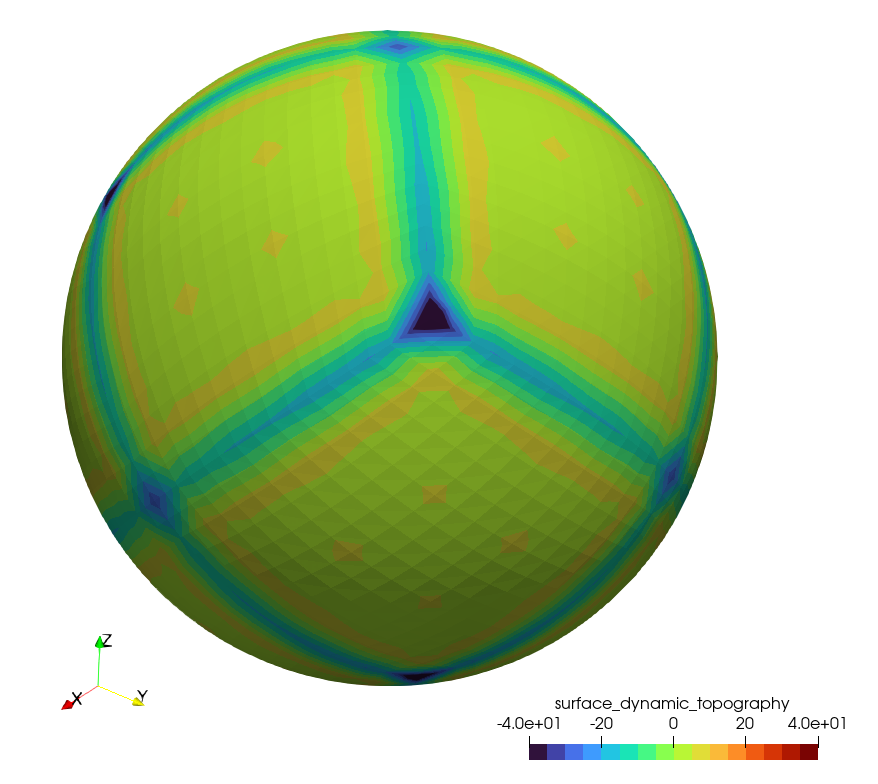
\includegraphics[width=5cm]{images/dyntopo/dyntopo.jpg}\\
{\captionfont Taken from \url{http://www.ga.gov.au/news-events/news/latest-news/dynamic-topography-of-australias-margins}}
\end{center}

\begin{small}
\begin{itemize}
\item[\nineteeneightyfive] 
\fullcite{hacr85} 
\item[\nineteeneightyseven] 
\fullcite{repa87} 
\item[\nineteenninetytwo] 
\fullcite{kiha92} 
\item[\nineteenninetythree] 
\fullcite{gurn93} \\
\fullcite{gurn93b}
\item[\nineteenninetyseven] 
\fullcite{pymi97} 
\item[\nineteenninetynine] 
\fullcite{bumo99} 
\item[\twothousand] 
\fullcite{paha00} \\
\fullcite{paha00b} 
\item[\twothousandone] 
\fullcite{pari01} 
\item[\twothousandthree] 
\fullcite{cogu03} 
\item[\twothousandseven] 
\fullcite{stei07} 
\item[\twothousandeight] 
\fullcite{mofm08} 
\item[\twothousandnine] 
\fullcite{cohu09} 
\item[\twothousandten] 
\fullcite{bofb10} \\
\fullcite{brau10} \\
\fullcite{stfh10} \\
\fullcite{shml10} 
\item[\twothousandeleven] 
\fullcite{rapy11} 
\item[\twothousandtwelve] 
\fullcite{shlm12} \\
\fullcite{zhzf12} 
\item[\twothousandthirteen] 
\fullcite{brrs13} \\
\fullcite{flgm13} 
\item[\twothousandfifteen] 
\fullcite{aupm15} \\
\fullcite{kiff15} \\
\fullcite{dali15} 
\item[\twothousandsixteen] 
\fullcite{howa16} \\
\fullcite{gvfb16} \\
\fullcite{yagu16} \\
\fullcite{stei16} \\
\fullcite{cogb16} 
\item[\twothousandseventeen] 
\fullcite{yamm17} \\
\fullcite{aumh17} \\
\fullcite{grrb17} \\
\fullcite{rubh17} \\
\fullcite{sekf17} 
\item[\twothousandeighteen] 
\fullcite{osss18} \\
\fullcite{vibc18} 
\item[\twothousandnineteen] 
\fullcite{deli19}\\
\fullcite{stco19}\\
\fullcite{davk19}\\
\fullcite{bore19}
\item[\twothousandtwenty] 
\fullcite{braf20}\\
\fullcite{kiso20}\\
\fullcite{miac20}
\item[\twothousandtwentyone] 
\fullcite{hoar21}
\item[\twothousandtwentytwo] 
\fullcite{holt22} \\
\fullcite{gurs22}
\item[\twothousandtwentythree] 
\fullcite{ropr23} \\
\fullcite{rich23} \\
\fullcite{tabs23}
\item[\twothousandtwentyfour]
\fullcite{wisa24} \\ 
\fullcite{vibb24} \\ 
\fullcite{cawc24} \\ 
\fullcite{omrp24} \\ 
\fullcite{stsb24} 
\item[\twothousandtwentyfive]
\fullcite{yawz25}
\end{itemize}
\end{small}

See also report/article written by Zhong (2018) \textcite{zhon18}

%------------------------------------------------------------------------------
%------------------------------------------------------------------------------
\section{cratons, cratonic roots}

\begin{small}
\begin{itemize}
\item[\nineteenninetyseven] 
\fullcite{bugm97} 
\item[\nineteenninetynine] 
\fullcite{drdv99} \\
\fullcite{lemo99} 
\item[\twothousand] 
\fullcite{kiri00} \\
\fullcite{lemm00} \\
\fullcite{scth00} 
\item[\twothousandone] 
\fullcite{brsh01} \\
\fullcite{drvc01} 
\item[\twothousandthree] 
\fullcite{lemm03} \\
\fullcite{wemv03} 
\item[\twothousandsix] 
\fullcite{coll06} 
\item[\twothousandeight] 
\fullcite{onlg08} 
\item[\twothousandnine] 
\fullcite{coco09} \\
\fullcite{kekj09} 
\item[\twothousandeleven] 
\fullcite{hube11}  \\
\fullcite{salo11} 
\item[\twothousandtwelve] 
\fullcite{gohg12} \\
\fullcite{gubc12} \\
\fullcite{mibe12} \\
\fullcite{yosh12} \\
\fullcite{pokb12} 
\item[\twothousandthirteen] 
\fullcite{frbm13} \\
\fullcite{gahs13} \\
\fullcite{ligw13} 
\item[\twothousandfourteen] 
\fullcite{gagb14} \\
\fullcite{wavp14} \\
\fullcite{baeg14} \\
\fullcite{comi14} \\
\fullcite{lige14} 
\item[\twothousandfifteen] 
\fullcite{wahz15} \\
\fullcite{wazh15} \\
\fullcite{tarn15} 
\item[\twothousandsixteen] 
\fullcite{wahz16} \\
\fullcite{kobc16} 
\item[\twothousandseventeen] 
\fullcite{liwg17} 
\item[\twothousandeighteen] 
\fullcite{rabw18} \\
\fullcite{bemc18} \\
\fullcite{gomb18} \\
\fullcite{webe18b} \\
\fullcite{wavp18} \\
\fullcite{lili18} \\
\fullcite{pagc19} 
\item[\twothousandtwenty] 
\fullcite{canc20} \\
\fullcite{cels20} \\
\fullcite{pegz20} \\
\fullcite{cofm20} \\
\fullcite{pagh20} 
\item[\twothousandtwentyone] 
\fullcite{becf21} \\ 
\fullcite{pelg21} \\ 
\fullcite{foon21} \\ 
\fullcite{sasa21} 
\item[\twothousandtwentytwo] 
\fullcite{canm22} \\
\fullcite{jarv22} \\ 
\fullcite{wacw22} 
\item[\twothousandtwentythree] 
\fullcite{wacp23} \\
\fullcite{gejb23} \\
\fullcite{pacb23}
\item[\twothousandtwentyfour] 
\fullcite{fuli24} \\
\fullcite{kucp24} \\
\fullcite{recf24} \\
\fullcite{comi24} \\
\fullcite{qicz24}
\end{itemize}
\end{small}

%------------------------------------------------------------------------------
%------------------------------------------------------------------------------
\section{Lithospheric stress, intra-plate stress, intra-plate deformation}
%------------------------------------------------------------------------------
%------------------------------------------------------------------------------

\begin{small}
\begin{itemize}
\item[\nineteenseventyfive] 
\fullcite{fouy75}\\
\fullcite{sosr75}
\item[\nineteenseventysix] 
\fullcite{riss76}
\item[\nineteenseventyseven] 
\fullcite{chtu77}
\item[\nineteenseventynine] 
\fullcite{riss79}
\item[\nineteeneightynine] 
\fullcite{boww89}
\item[\nineteenninetyone] 
\fullcite{worg91}
\item[\nineteenninetytwo] 
\fullcite{rich92}\\
\fullcite{wuvr92}\\
\fullcite{zoba92}\\
\fullcite{gowc92}\\
\fullcite{clko92}
\item[\nineteenninetynine] 
\fullcite{bili99}
\item[\twothousandone] 
\fullcite{stsm01}
\item[\twothousandtwo] 
\fullcite{jack02}
\item[\twothousandfour] 
\fullcite{ligu04} \\
\fullcite{buja04}
\item[\twothousandfive] 
\fullcite{timr05}
\item[\twothousandseven] 
\fullcite{hert07}
\item[\twothousandeight] 
\fullcite{bilr08}\\
\fullcite{ghhw08}\\
\fullcite{netv08}
\item[\twothousandnine] 
\fullcite{ghhf09}\\
\fullcite{nacl09}\\
\fullcite{kalb09}
\item[\twothousandten] 
\fullcite{bepo10}\\
\fullcite{yosh10}
\item[\twothousandtwelve] 
\fullcite{nalr12}\\
\fullcite{ghho12}\\
\fullcite{wagw12}
\item[\twothousandthirteen] 
\fullcite{ghhw13}
\item[\twothousandfourteen] 
\fullcite{vagw14}
\item[\twothousandseventeen] 
\fullcite{grrb17}
\item[\twothousandeighteen] 
\fullcite{osss18}\\
\fullcite{magu18}
\item[\twothousandnineteen] 
\fullcite{tamg19}
\item[\twothousandtwentyone]
\fullcite{poyd21} 
\end{itemize}
\end{small}


%--------------------------------------------------------------------
%------------------------------------------------------------------------------
\section{passive margins} 
%--------------------------------------------------------------------
%------------------------------------------------------------------------------

\begin{small}
\begin{itemize}
\item[\nineteeneightytwo] 
\fullcite{clwv82} 
\item[\nineteeneightysix] 
\fullcite{lies86} 
\item[\twothousandfive] 
\fullcite{gebi05} 
\item[\twothousandeight] 
\fullcite{clbz08} \\
\fullcite{kasb08} 
\item[\twothousandten] 
\fullcite{fasm10} \\
\fullcite{nigm10} 
\item[\twothousandeleven] 
\fullcite{rapy11} \\
\fullcite{nigm11} \\
\fullcite{brfo11} 
\item[\twothousandthirteen] 
\fullcite{mana13} \\
\fullcite{yahb13} 
\item[\twothousandfourteen] 
\fullcite{macg14} 
\item[\twothousandfifteen] 
\fullcite{gebw15} \\
\fullcite{nigo15} 
\item[\twothousandsixteen] 
\fullcite{dupm16} 
\item[\twothousandeighteen] 
\fullcite{sahf18} \\
\fullcite{mube18} \\
\fullcite{tebu18} 
\item[\twothousandnineteen] 
\fullcite{zhli19} 
\item[\twothousandtwentyone] 
\fullcite{auws21} 
\item[\twothousandtwentytwo] 
\fullcite{bagm22}
\end{itemize}
\end{small}

%------------------------------------------------------------------------------
%------------------------------------------------------------------------------
\section{Eclogites} 
%------------------------------------------------------------------------------
%------------------------------------------------------------------------------

\begin{small}
\begin{itemize}
\item[\twothousandone] 
\fullcite{dohe01} 
\item[\twothousandseven] 
\fullcite{hecb07} 
\item[\twothousandnine] 
\fullcite{agyj09} 
\item[\twothousandthirteen] 
\fullcite{arbi13} \\
\fullcite{krcu13} 
\item[\twothousandtwentytwo] 
\fullcite{wakw22}\\ 
\fullcite{yadb22} 
\end{itemize}
\end{small}


%--------------------------------------------------------------------
%------------------------------------------------------------------------------
\section{Folding, buckling} 
%--------------------------------------------------------------------
%------------------------------------------------------------------------------

\begin{small}
\begin{itemize}
\item[\nineteenseventy] 
\fullcite{ramb70} 
\item[\nineteenseventyone] 
\fullcite{ramb71} 
\item[\nineteenseventyeight] 
\fullcite{wilz78} 
\item[\nineteenninetyone] 
\fullcite{flet91}\\ 
\fullcite{wiwh91} 
\item[\nineteenninetythree] 
\fullcite{zhhj93} 
\item[\nineteenninetyfive] 
\fullcite{flet95} 
\item[\nineteenninetysix] 
\fullcite{zhho96} 
\item[\nineteenninetynine] 
\fullcite{nagg99}\\ 
\fullcite{bupo99} \\
\fullcite{scpo99} 
\item[\twothousandone] 
\fullcite{scpo01} \\
\fullcite{scpo01b} 
\item[\twothousandtwo] 
\fullcite{mumh02} 
\item[\twothousandthree] 
\fullcite{ribe03} \\
\fullcite{nagv03} 
\item[\twothousandsix] 
\fullcite{frsc06} 
\item[\twothousandseven] 
\fullcite{risr07} 
\item[\twothousandeight] 
\fullcite{schm08} \\
\fullcite{manc08} \\
\fullcite{scdk08} 
\item[\twothousandnine] 
\fullcite{simp09} 
\item[\twothousandten] 
\fullcite{resb10} 
\item[\twothousandeleven] 
\fullcite{freh11} 
\item[\twothousandtwelve] 
\fullcite{reds12} \\
\fullcite{grsc12} \\
\fullcite{scsc12} 
\item[\twothousandthirteen] 
\fullcite{regc13} 
\item[\twothousandfourteen] 
\fullcite{freh14} \\
\fullcite{frex14} 
\item[\twothousandsixteen] 
\fullcite{frsc16} 
\item[\twothousandtwentyone] 
\fullcite{nafo21} 
\item[\twothousandtwentythree] 
\fullcite{dosk23} 
\end{itemize}
\end{small}

%--------------------------------------------------------------------
%------------------------------------------------------------------------------
\section{geoid}
%--------------------------------------------------------------------
%------------------------------------------------------------------------------

\begin{small}
\begin{itemize}
\item[\nineteeneightyfour] 
\fullcite{davi84} \\
\fullcite{hage84} \\
\fullcite{riff84} \\
\fullcite{riha84} \\
\fullcite{wari84} 
\item[\nineteeneightyfive] 
\fullcite{hacr85}\\ 
\fullcite{chas85} 
\item[\nineteeneightysix] 
\fullcite{davi86} 
\item[\nineteeneightyseven] 
\fullcite{fope87} 
\item[\nineteeneightyeight] 
\fullcite{besz88} \\
\fullcite{fope88} 
\item[\nineteeneightynine] 
\fullcite{rivf89} \\
\fullcite{hari89}
\item[\nineteenninetyone] 
\fullcite{mocf91}
\item[\nineteenninetytwo] 
\fullcite{zhgu92} \\
\fullcite{kiha92} \\
\fullcite{ribe92} 
\item[\nineteenninetythree] 
\fullcite{zhch93} \\
\fullcite{rirl93} 
\item[\nineteenninetyfour] 
\fullcite{kiha94} 
\item[\nineteenninetyfive] 
\fullcite{king95} \\
\fullcite{pape95} \\
\fullcite{mopa95} \\
\fullcite{thmc95} 
\item[\nineteenninetysix]  
\fullcite{mogu96} \\
\fullcite{kafl96} \\
\fullcite{pape96} \\
\fullcite{dofm96} \\
\fullcite{pahf96} 
\item[\nineteenninetyseven] 
\fullcite{wean97a} \\
\fullcite{king97} \\
\fullcite{thri97} 
\item[\nineteenninetyeight] 
\fullcite{cava98} \\
\fullcite{chki98} \\
\fullcite{kike98} 
\item[\twothousand] 
\fullcite{dofl00} \\
\fullcite{kafl00} \\
\fullcite{paha00} 
\item[\twothousandone] 
\fullcite{zhon01} 
\item[\twothousandtwo] 
\fullcite{peso02} 
\item[\twothousandseven] 
\fullcite{kart07} 
\item[\twothousandeight] 
\fullcite{meco08} 
\item[\twothousandnine] 
\fullcite{king09} \\
\fullcite{tocm09} \\
\fullcite{yona09} 
\item[\twothousandten] 
\fullcite{ghbz10}\\
\fullcite{spgs10b}
\item[\twothousandeleven] 
\fullcite{capd11}
\item[\twothousandtwelve] 
\fullcite{hibi12}\\
\fullcite{cabp12}\\
\fullcite{katr12}
\item[\twothousandthirteen] 
\fullcite{shsc13}\\
\fullcite{chus13}
\item[\twothousandfourteen] 
\fullcite{cako14}\\
\fullcite{kaps14}
\item[\twothousandfifteen] 
\fullcite{lizh15}
\item[\twothousandsixteen] 
\fullcite{necg16}
\fullcite{lizh16}
\item[\twothousandseventeen] 
\fullcite{grab17}\\
\fullcite{siag17}
\item[\twothousandeighteen] 
\fullcite{king18}
\item[\twothousandtwentyone]
\fullcite{mazh21b} 
\item[\twothousandtwentytwo]
\fullcite{rojy22}\\
\fullcite{ghpa22}\\
\fullcite{licw22}
\item[\twothousandtwentythree]
\fullcite{stgl23} \\
\fullcite{saaf23} \\
\fullcite{pagh23}
\end{itemize}
\end{small}

%--------------------------------------------------------------------
%------------------------------------------------------------------------------
\section{geothermal Energy} 
%--------------------------------------------------------------------
%------------------------------------------------------------------------------

\begin{small}
\begin{itemize}
\item[\twothousandfifteen]
\fullcite{quxm15} 
\item[\twothousandnineteen]
\fullcite{revf19} 
\end{itemize}
\end{small}

%--------------------------------------------------------------------
%------------------------------------------------------------------------------
\section{grain size (evolution) \& influence on geodynamics}
\label{sec:topics:gsev}
%--------------------------------------------------------------------
%------------------------------------------------------------------------------

\begin{small}
\begin{itemize}
\item[\nineteeneightyfour] 
\fullcite{kara84} 
\item[\nineteenninetysix] 
\fullcite{solo96} 
\item[\nineteenninetyseven] 
\fullcite{kayf97} 
\item[\nineteeneightynine] 
\fullcite{brcp99} 
\item[\twothousandone] 
\fullcite{dets01} \\
\fullcite{solo01} 
\item[\twothousandtwo] 
\fullcite{soet02} 
\item[\twothousandthree] 
\fullcite{hapa03} \\
\fullcite{reyu03} 
\item[\twothousandeight] 
\fullcite{sore08} 
\item[\twothousandnine] 
\fullcite{behe09} 
\item[\twothousandeleven] 
\fullcite{rorb11} 
\item[\twothousandtwelve]
\fullcite{fobl12} 
\item[\twothousandthirteen] 
\fullcite{beri13} 
\item[\twothousandfourteen] 
\fullcite{fobe14} 
\item[\twothousandfifteen] 
\fullcite{thrk15} \\
\fullcite{besr15} \\
\fullcite{tukb15} \\
\fullcite{pevp15} \\
\fullcite{glfa15} 
\item[\twothousandseventeen] 
\fullcite{ceww17} \\
\fullcite{daef17} \\
\fullcite{mube17} \\
\fullcite{fori17} \\
\fullcite{scdu17} 
\item[\twothousandeighteen] 
\fullcite{bemu18} \\
\fullcite{bezb18} \\
\fullcite{mube18} \\
\fullcite{jakk18} \\
\fullcite{fole18} 
\item[\twothousandnineteen] 
\fullcite{mube19} 
\item[\twothousandtwenty] 
\fullcite{mube20} \\
\fullcite{scrt20}\\
\fullcite{sctr20} \\
\fullcite{thsc20} \\
\fullcite{fole20} \\
\fullcite{sctp20} 
\item[\twothousandtwentyone]
\fullcite{mazh21a}  \\ 
\fullcite{fube21} 
\item[\twothousandtwentytwo]
\fullcite{rutb22} 
\item[\twothousandtwentythree]
\fullcite{racs23} 
\item[\twothousandtwentyfour]
\fullcite{pagr24} 
\end{itemize}
\end{small}

%--------------------------------------------------------------------
%------------------------------------------------------------------------------
\section{LLSVP, ULVZ, CMB layer, thermo-chemical piles, D'' layer}
%------------------------------------------------------------------------------
%--------------------------------------------------------------------

\begin{center}
\includegraphics[width=5cm]{images/burk11}\cite{burk11}
\end{center}

\begin{small}
\begin{itemize}
\item[\nineteeneighty]       
\fullcite{yupe80} 
\item[\nineteeneightysix]    
\fullcite{dagu86} 
\item[\nineteeneightyeight]  
\fullcite{hayu88} 
\item[\nineteeneightynine]   
\fullcite{hayu89} 
\item[\nineteenninetyfour]   
\fullcite{ride94} 
\item[\nineteenninetysix]    
\fullcite{boeh96} 
\item[\nineteenninetyseven]  
\fullcite{kell97} 
\item[\nineteenninetyeight]  
\fullcite{tack98b} 
\item[\twothousand]
\fullcite{moke00} 
\item[\twothousandone]       
\fullcite{soga01} 
\item[\twothousandtwo]       
\fullcite{somo02} \\
\fullcite{tagh02} 
\item[\twothousandthree]
\fullcite{zhha03}
\item[\twothousandfour]      
\fullcite{mczh04} \\
\fullcite{nata04} 
\item[\twothousandfive]      
\fullcite{nata05} \\
\fullcite{wyso05} \\
\fullcite{mczh05a} \\
\fullcite{nata05b}
\item[\twothousandsix]       
\fullcite{nata06} 
\item[\twothousandseven]     
\fullcite{heta07}\\
\fullcite{moyu07} \\
\fullcite{pelt07} \\
\fullcite{hibl07} \\
\fullcite{yumc07} 
\item[\twothousandeight]     
\fullcite{gamc08} \\
\fullcite{nata08} \\
\fullcite{stho08} 
\item[\twothousandnine]
\fullcite{bumr09} 
\item[\twothousandten]
\fullcite{stto10} \\
\fullcite{mcgr10} \\
\fullcite{nata10} \\
\fullcite{vady10} \\
\fullcite{toyc10} 
\item[\twothousandeleven]    
\fullcite{bowg11} \\
\fullcite{talz11} \\
\fullcite{vayj11} \\
\fullcite{dekt11} \\
\fullcite{burk11} 
\item[\twothousandtwelve]    
\fullcite{stto12} \\
\fullcite{dagd12} \\
\fullcite{dect12} 
\item[\twothousandthirteen]  
\fullcite{limc13} \\
\fullcite{bogs13a} \\
\fullcite{bogs13b} 
\item[\twothousandfourteen]  
\fullcite{budt14} \\
\fullcite{lidt14} \\
\fullcite{tovd14} 
\item[\twothousandfifteen]   
\fullcite{musd15} \\
\fullcite{hafg15} \\
\fullcite{delt15} \\
\fullcite{wilm15} \\
\fullcite{lidt15} \\
\fullcite{sobd15} \\
\fullcite{dagl15} 
\item[\twothousandsixteen]   
\fullcite{dost16} \\
\fullcite{tosa16} 
\item[\twothousandseventeen] 
\fullcite{hish17} \\
\fullcite{lizh17} \\
\fullcite{limg17} \\
\fullcite{siag17} 
\item[\twothousandeighteen]  
\fullcite{daga18} \\
\fullcite{lizo18} \\
\fullcite{hect18} \\
\fullcite{dert18} 
\item[\twothousandnineteen]  
\fullcite{hebo19} \\
\fullcite{rejv19} \\
\fullcite{mcna19} 
\item[\twothousandtwenty]    
\fullcite{cilw20} \\
\fullcite{szes20} \\
\fullcite{scrt20} \\
\fullcite{daro20} \\
\fullcite{hect20b} 
\item[\twothousandtwentyone]
\fullcite{cafb21} \\
\fullcite{damg21} 
\item[\twothousandtwentytwo] 
\fullcite{limc22} \\
\fullcite{yuli22} \\
\fullcite{flbw22}\\
\fullcite{lalt22}\\
\fullcite{hulz22} 
\item[\twothousandtwentythree] 
\fullcite{hagl23} \\
\fullcite{gudl23} \\
\fullcite{padm23} \\
\fullcite{lizl23}
\item[\twothousandtwentyfour] 
\fullcite{bero24} \\
\fullcite{shml24} \\
\fullcite{liwg24} \\
\fullcite{deba24} \\
\fullcite{roy}
\item[\twothousandtwentyfive] 
\fullcite{padk25} \\
\fullcite{hedg25} \\
\fullcite{rosf25} \\
\fullcite{hugu25}
\end{itemize}
\end{small}

%--------------------------------------------------------------------
%------------------------------------------------------------------------------
\section{magma ocean}
%--------------------------------------------------------------------
%------------------------------------------------------------------------------

\begin{small}
\begin{itemize}
\item[\nineteenninetythree] 
\fullcite{sost93a} \\
\fullcite{sost93b} 
\item[\twothousandtwo] 
\fullcite{elvh02} 
\item[\twothousandsix] 
\fullcite{hosh06}
\item[\twothousandseven] 
\fullcite{solo07} 
\item[\twothousandten] 
\fullcite{devv10} 
\item[\twothousandtwelve] 
\fullcite{ullc12} 
\item[\twothousandthirteen] 
\fullcite{plth13} \\
\fullcite{moha13} 
\item[\twothousandfifteen] 
\fullcite{maha15} 
\item[\twothousandseventeen] 
\fullcite{mats17} \\ 
\fullcite{bori17} 
\item[\twothousandtwenty] 
\fullcite{bobm20} \\
\fullcite{agml20} 
\item[\twothousandtwentythree] 
\fullcite{sasa23} 
\item[\twothousandtwentyfive] 
\fullcite{bobs25} 
\end{itemize}
\end{small}

%------------------------------------------------------------------------------
%------------------------------------------------------------------------------
\section{magmatic arcs, arc volcanism}
%------------------------------------------------------------------------------
%------------------------------------------------------------------------------

\begin{small}
\begin{itemize}
\item[1982] \fullcite{crpi82}
\item[2015] \fullcite{cudd15}
\item[2017] \fullcite{sche17}\\ \fullcite{lewa17}
\item[2025] \fullcite{masg25}
\end{itemize}
\end{small}



%------------------------------------------------------------------------------
%------------------------------------------------------------------------------
\section{magma transport / melting / two-phase flow/ (intra-plate) 
volcanism / lava flow/ continental flood basalt, melt migration}
%------------------------------------------------------------------------------
%------------------------------------------------------------------------------

\begin{small}
\begin{itemize}
\item[\nineteeneightyfour] 
\fullcite{scst84} \\
\fullcite{mcke84} 
\item[\nineteeneightyfive] 
\fullcite{ribe85} \\
\fullcite{ribe85b} 
\item[\nineteeneightysix] 
\fullcite{scst86} \\
\fullcite{ribe86} 
\item[\nineteeneightyseven] 
\fullcite{hayu87} \\
\fullcite{spmc87} \\
\fullcite{rism87} \\
\fullcite{ribe87} 
\item[\nineteeneightyeight] 
\fullcite{scot88} \\
\fullcite{ribe88b} 
\item[\nineteeneightynine]
\fullcite{scst89} 
\item[\nineteenninety] 
\fullcite{hayu90} 
\item[\nineteenninetythree] 
\fullcite{spie93} \\
\fullcite{tast93} 
\item[\nineteenninetyfour] 
\fullcite{jhpp94} \\
\fullcite{sawy94} 
\item[\nineteenninetyfive] 
\fullcite{bisc95} \\
\fullcite{crks95} \\
\fullcite{ahwk95} 
\item[\nineteenninetysix] 
\fullcite{laki96} 
\item[\nineteenninetyeight] 
\fullcite{rabg98} 
\item[\nineteenninetynine] 
\fullcite{devv99} \\
\fullcite{momo99} 
\item[\twothousand] 
\fullcite{elha00} 
\item[\twothousandone] 
\fullcite{bers01} 
\item[\twothousandtwo] 
\fullcite{sobo02} 
\item[\twothousandthree] 
\fullcite{beri03} 
\item[\twothousandfive] 
\fullcite{onml05} \\
\fullcite{likc05} 
\item[\twothousandsix] 
\fullcite{onmm06} 
\item[\twothousandseven] 
\fullcite{srrb07} \\
\fullcite{mohb07} \\
\fullcite{elki07} \\
\fullcite{onlj07} \\
\fullcite{copb07} 
\item[\twothousandeight] 
\fullcite{hets08} \\
\fullcite{hest08} 
\item[\twothousandnine] 
\fullcite{bavi09} 
\item[\twothousandten] 
\fullcite{baiv10} \\
\fullcite{habl10} \\
\fullcite{cows10} \\
\fullcite{dekc10} 
\item[\twothousandeleven] 
\fullcite{baiv11} \\
\fullcite{zhgy11} \\
\fullcite{zhgh11} \\
\fullcite{bics11} \\
\fullcite{mobh11} 
\item[\twothousandtwelve] 
\fullcite{yatd12} \\
\fullcite{kasc12b} \\
\fullcite{ullc12} \\
\fullcite{plsp12} \\
\fullcite{kawe12} 
\item[\twothousandthirteen] 
\fullcite{kemk13} \\
\fullcite{mofm13} \\
\fullcite{plbs13} \\
\fullcite{mowe13} 
\item[\twothousandfourteen] 
\fullcite{kast14} 
\item[\twothousandfifteen] 
\fullcite{tukb15} \\
\fullcite{moba15} \\
\fullcite{rerl15} \\
\fullcite{riag15} \\
\fullcite{rey15} \\
\fullcite{yadm15} 
\item[\twothousandsixteen] 
\fullcite{keka16} \\
\fullcite{vade16} \\
\fullcite{mesj16} \\
\fullcite{dalg16} \\
\fullcite{libz16} \\
\fullcite{rogj16} \\
\fullcite{porb16} 
\item[\twothousandseventeen] 
\fullcite{dilc17} \\
\fullcite{arca17} \\
\fullcite{mova17} \\
\fullcite{mosw17} 
\item[\twothousandeighteen] 
\fullcite{mova18} \\
\fullcite{lorg18} \\
\fullcite{scmo18} \\ 
\fullcite{yaca18} \\ 
\fullcite{pegp18} \\ 
\fullcite{govo18} \\ 
\fullcite{shi_thesis}
\item[\twothousandnineteen] 
\fullcite{dagg19} \\
\fullcite{scmw19} \\
\fullcite{kesu19} \\
\fullcite{cerk19} \\
\fullcite{likk19} \\
\fullcite{jart19b} 
\item[\twothousandtwenty] 
\fullcite{siss20} \\
\fullcite{zhbp20} \\
\fullcite{rubk20} \\
\fullcite{rukb20} \\
\fullcite{cobd20} \\
\fullcite{spkh20} \\ 
\fullcite{spkh20b} \\ 
\fullcite{lerm20} 
\item[\twothousandtwentyone] 
\fullcite{dudm21} \\
\fullcite{damg21} 
\item[\twothousandtwentytwo] 
\fullcite{kajr22} \\
\fullcite{zhlz22} \\
\fullcite{bepp22} \\
\fullcite{vacd22} \\
\fullcite{kilk22} \\
\fullcite{kosl22}
\item[\twothousandtwentythree]
\fullcite{kimk23} \\ 
\fullcite{scmw23} \\ 
\fullcite{xumm23} \\
\fullcite{mahs23} \\
\fullcite{yole23}
\item[\twothousandtwentyfour] 
\fullcite{lumh24} \\
\fullcite{hesc24} \\
\fullcite{lech24} \\
\fullcite{mori24} \\
\fullcite{tibi24} 
\item[2025]
\fullcite{puld25}
\end{itemize}
\end{small}

%--------------------------------------------------------------------
%--------------------------------------------------------------------
\section{magma chambers}
%--------------------------------------------------------------------
%--------------------------------------------------------------------

\begin{small}
\begin{itemize}
\item[\nineteeneightytwo] 
\fullcite{spyk82} 
\item[\nineteeneightyseven] 
\fullcite{hayu87} 
\item[\twothousandfour] 
\fullcite{geys04} 
\item[\twothousandnine] 
\fullcite{vesc09} 
\item[\twothousandtwelve] 
\fullcite{gerb12} \\
\fullcite{gech12} 
\item[\twothousandfourteen] 
\fullcite{cuwi14} 
\item[\twothousandeighteen] 
\fullcite{gehn18} 
\end{itemize}
\end{small}

%--------------------------------------------------------------------
%------------------------------------------------------------------------------
\section{mantle convection/dynamics, whole Earth models, plate interaction}
%--------------------------------------------------------------------
%------------------------------------------------------------------------------

\begin{small}
\begin{itemize}
\item[\nineteensixtyseven] 
\fullcite{tuox67} 
\item[\nineteensixtynine] 
\fullcite{tuox69} 
\item[\nineteenseventyone] 
\fullcite{totu71b} \\
\fullcite{totu71} \\
\fullcite{buwh71} 
\item[\nineteenseventytwo] 
\fullcite{pelt72} \\ 
\fullcite{hstt72} \\ 
\fullcite{sctu72} 
\item[\nineteenseventythree] 
\fullcite{mcrw73} \\ 
\fullcite{rich73b} 
\item[\nineteenseventyfour] 
\fullcite{youn74} \\
\fullcite{tuht74} \\
\fullcite{trol94}\\
\fullcite{mcrw74} 
\item[\nineteenseventyfive] 
\fullcite{hemw75} \\
\fullcite{buss75} 
\item[\nineteenseventysix] 
\fullcite{mcri76} \\
\fullcite{patt76} \\
\fullcite{sath76} 
\item[\nineteenseventyseven] 
\fullcite{yusc77} 
\item[\nineteenseventyeight] 
\fullcite{mahz78} \\
\fullcite{hsui78} \\
\fullcite{haoc78} \\
\fullcite{pamc78} \\
\fullcite{jaco78} \\
\fullcite{rimc78} 
\item[\nineteenseventynine] 
\fullcite{ludt79} \\
\fullcite{buss79} \\
\fullcite{shpe79} \\
\fullcite{phiv79} 
\item[\nineteeneighty] 
\fullcite{olco80} \\
\fullcite{jamc80} \\
\fullcite{scsc80} \\
\fullcite{zess80} \\
\fullcite{daly80} 
\item[\nineteeneightyone] 
\fullcite{yups81} \\
\fullcite{buss81} \\
\fullcite{jasc81} \\
\fullcite{jape81} \\
\fullcite{haoc81} \\
\fullcite{rimc81} \\
\fullcite{cotu81} 
\item[\nineteeneightytwo] 
\fullcite{jape82} \\
\fullcite{jasc82} \\
\fullcite{homc82} \\
\fullcite{buri82} 
\item[\nineteeneightythree] 
\fullcite{hous83} \\
\fullcite{hous83b} \\
\fullcite{chri83} \\
\fullcite{chri83b} \\
\fullcite{mcke83} \\
\fullcite{boss83} \\
\fullcite{zesd83} 
\item[\nineteeneightyfour] 
\fullcite{olyb84} \\
\fullcite{jarv84} \\
\fullcite{haeb84} \\
\fullcite{haeb84b} \\
\fullcite{harp84} \\
\fullcite{davi84} \\
\fullcite{boas84} \\
\fullcite{chri84} \\
\fullcite{chri84b} \\
\fullcite{moca84}\\
\fullcite{flyu84} \\
\fullcite{jarv84} \\
\fullcite{flyu84b} 
\item[\nineteeneightyfive] 
\fullcite{jarv85} \\
\fullcite{baum85} \\
\fullcite{chri85} \\
\fullcite{csra85} \\
\fullcite{scan85} 
\item[\nineteeneightysix] 
\fullcite{davi86} \\
\fullcite{guda86} \\
\fullcite{quys86} \\
\fullcite{jape86} \\
\fullcite{crmc86} 
\item[\nineteeneightyseven] 
\fullcite{yuqh87} \\ 
\fullcite{olso87} \\ 
\fullcite{mija87} \\ 
\fullcite{chri87b} 
\item[\nineteeneightyeight] 
\fullcite{haeb88} \\
\fullcite{glat88} \\
\fullcite{gurn88} \\
\fullcite{viyu88} \\
\fullcite{whit88} \\
\fullcite{davi88} \\
\fullcite{csrr88} \\
\fullcite{elsc88} \\
\fullcite{grpa98} 
\item[\nineteeneightynine] 
\fullcite{weoy89} \\
\fullcite{chyu89} \\
\fullcite{besg89} \\
\fullcite{schm89} \\
\fullcite{sthe89} \\
\fullcite{rivi89} \\
\fullcite{chri89b} \\
\fullcite{jami89} \\
\fullcite{davi89} 
\item[\nineteenninety] 
\fullcite{trab90} \\
\fullcite{gurn90} \\
\fullcite{ketu90} \\
\fullcite{jape90} \\
\fullcite{sope90} 
\item[\nineteenninetyone] 
\fullcite{jarv91} \\
\fullcite{chha91} \\
\fullcite{mawe91} \\
\fullcite{gaot91} \\
\fullcite{vayv91} \\
\fullcite{hayk91} \\
\fullcite{leys91} \\
\fullcite{virf91} \\
\fullcite{mayu91} 
\item[\nineteenninetytwo] 
\fullcite{dari92} \\
\fullcite{besg92} \\
\fullcite{vayv92} \\
\fullcite{chri92} \\
\fullcite{haym92} \\
\fullcite{rien92} \\
\fullcite{hayk92} \\
\fullcite{mayw92} \\
\fullcite{mayu92} 
\item[\nineteenninetythree] 
\fullcite{bayr93} \\
\fullcite{zhch93} \\
\fullcite{jarv93} \\
\fullcite{tack93} \\
\fullcite{carm93} \\
\fullcite{vavy93} \\
\fullcite{tasg93} \\
\fullcite{zhgu93} \\
\fullcite{mamc93} \\
\fullcite{zebi93} \\
\fullcite{vayv93} \\
\fullcite{hayk93} \\
\fullcite{hayu93} \\
\fullcite{hoyb93} \\
\fullcite{hoby93} 
\item[\nineteenninetyfour] 
\fullcite{yurb94} \\
\fullcite{bayu94} \\
\fullcite{haeb94} \\
\fullcite{bucc94} \\
\fullcite{chho94} \\
\fullcite{tasg94} \\
\fullcite{past94} \\
\fullcite{itki94} \\
\fullcite{leka94} \\
\fullcite{sope94} \\
\fullcite{sope94b} \\
\fullcite{jarv94} \\
\fullcite{vaja94} \\
\fullcite{scha94} 
\item[\nineteenninetyfive] 
\fullcite{styu95} \\
\fullcite{bayr95} \\
\fullcite{bayr95b} \\
\fullcite{zhgu95} \\
\fullcite{vayv95} \\
\fullcite{buba95} \\
\fullcite{rasz95} \\
\fullcite{guja95} \\
\fullcite{berc95} \\
\fullcite{puhj95} \\
\fullcite{pujh95} \\
\fullcite{solo95} \\
\fullcite{vayu95} \\
\fullcite{matb95} \\
\fullcite{vayp95} \\
\fullcite{jagv95} \\
\fullcite{jarv95} \\
\fullcite{thmc95} 
\item[\nineteenninetysix] 
\fullcite{laym96} \\
\fullcite{zhyu96} \\
\fullcite{hond96} \\
\fullcite{rytr96a}\\
\fullcite{rytr96b}\\
\fullcite{tack96}\\
\fullcite{trbo96} \\
\fullcite{birg96} \\
\fullcite{burb96} \\
\fullcite{kafo96} \\
\fullcite{guez96} \\
\fullcite{vayu96} \\
\fullcite{rasz96} \\
\fullcite{rasz96b} \\
\fullcite{leka96} \\
\fullcite{iwas96} \\
\fullcite{buri96} \\
\fullcite{schh96} \\
\fullcite{mora96} \\
\fullcite{trha96} 
\item[\nineteenninetyseven] 
\fullcite{deja97} \\
\fullcite{hond97} \\
\fullcite{iwho97} \\
\fullcite{burb97} \\
\fullcite{mole97} \\
\fullcite{somo97} \\
\fullcite{rats97} \\
\fullcite{cicv97} \\
\fullcite{vayu97} \\
\fullcite{laym97} \\
\fullcite{mebr97} \\
\fullcite{csyu97} \\
\fullcite{wahe97} \\
\fullcite{dofc97} 
\item[\nineteenninetyeight] 
\fullcite{ande98} \\
\fullcite{iwho98} \\
\fullcite{devv98} \\
\fullcite{tack98} \\
\fullcite{tack98b} \\
\fullcite{trha98b} \\
\fullcite{trha98} \\
\fullcite{burl98} \\
\fullcite{mokm98} \\
\fullcite{lena98} \\
\fullcite{vayu98} \\
\fullcite{wema98} \\
\fullcite{vaba98} 
\item[\nineteenninetynine] 
\fullcite{resb99} \\
\fullcite{duyr99} \\
\fullcite{vazh99} \\
\fullcite{dava99} \\
\fullcite{tabg99} \\
\fullcite{como99} \\
\fullcite{cicv99} \\
\fullcite{trrj99} \\
\fullcite{loga99} \\
\fullcite{sola99} \\
\fullcite{momo99} 
\item[\twothousand] 
\fullcite{albe00} \\
\fullcite{hayu00} \\
\fullcite{devv00b} \\
\fullcite{tack00} \\
\fullcite{tack00b} \\
\fullcite{tack00c} \\
\fullcite{tack00d} \\
\fullcite{zhzm00} \\
\fullcite{legm00} \\
\fullcite{conr00} \\
\fullcite{somo00} \\
\fullcite{duyu00} \\
\fullcite{duyy00} 
\item[\twothousandone] 
\fullcite{vank01} \\
\fullcite{riyb01} \\
\fullcite{lemo01} \\
\fullcite{vays01} \\
\fullcite{moqu01} \\
\fullcite{zhon01} \\
\fullcite{burm01} \\
\fullcite{dabu01} 
\item[\twothousandtwo] 
\fullcite{tasu02} \\
\fullcite{modm02} \\
\fullcite{tack02} \\
\fullcite{vaya02} \\
\fullcite{vayu02} \\
\fullcite{taxi02} \\
\fullcite{scbh02} \\
\fullcite{strb02} \\
\fullcite{duyr02} \\
\fullcite{hiys02} \\
\fullcite{alva02} 
\item[\twothousandthree] 
\fullcite{hapa03} \\
\fullcite{lemo03} \\
\fullcite{mumc03} \\
\fullcite{fasa03} \\
\fullcite{heta03} \\
\fullcite{sibu03} \\
\fullcite{ogaw03} \\
\fullcite{ogaw03b} \\
\fullcite{kore03} 
\item[\twothousandfour] 
\fullcite{thkl04} \\
\fullcite{vavv04b} \\
\fullcite{xita04b} \\
\fullcite{xita04} \\
\fullcite{nata04b} \\
\fullcite{vayr04} \\
\fullcite{brws04} \\
\fullcite{stsh04} \\
\fullcite{scbh04} \\
\fullcite{wahb04} \\
\fullcite{leda04} \\
\fullcite{leda04b} 
\item[\twothousandfive]
\fullcite{resb05}\\
\fullcite{wahb05} \\
\fullcite{taxn05}\\
\fullcite{bupc05} \\
\fullcite{grlt05} \\
\fullcite{lemj05} \\
\fullcite{kogk05} \\
\fullcite{mczh05b}\\
\fullcite{vary05} \\
\fullcite{nata05} \\
\fullcite{nabu05} \\
\fullcite{chob05} \\
\fullcite{phbu05} \\
\fullcite{hosh05} \\
\fullcite{funk05} 
\item[\twothousandsix] 
\fullcite{soba06} \\
\fullcite{beck06} \\
\fullcite{nake06} \\
\fullcite{losh06} \\
\fullcite{sthh06} \\
\fullcite{yoka06} \\
\fullcite{wahb06} \\
\fullcite{gowh06} 
\item[\twothousandseven] 
\fullcite{ghja07} \\
\fullcite{nake07} \\
\fullcite{mayu07} \\
\fullcite{brva07a} \\
\fullcite{brva07b} \\
\fullcite{grlt07} \\
\fullcite{grlt07b}\\
\fullcite{huda07} \\
\fullcite{tanh07} \\
\fullcite{tagu07} \\
\fullcite{jalo07} \\
\fullcite{galo07} \\
\fullcite{galo07b} \\
\fullcite{nelo07} \\
\fullcite{soba07} 
\item[\twothousandeight] 
\fullcite{ghja08} \\
\fullcite{tack08} \\
\fullcite{tack08b} \\
\fullcite{chhl08} \\
\fullcite{brhv08} \\
\fullcite{deta08} \\
\fullcite{plva08} \\
\fullcite{hole08} \\
\fullcite{vata08} \\
\fullcite{trkr08} \\
\fullcite{shlj08} \\
\fullcite{stha08} \\
\fullcite{yosh08} \\
\fullcite{galg08} 
\item[\twothousandnine] 
\fullcite{wodd09} \\
\fullcite{fobe09} \\
\fullcite{gows09} \\
\fullcite{deta09} \\
\fullcite{onlj09} \\
\fullcite{wazh09} \\
\fullcite{vavv09} \\
\fullcite{brha09} \\
\fullcite{scbs09b} \\
\fullcite{oebm09} \\
\fullcite{fuog09} 
\item[\twothousandten] 
\fullcite{oflo10} \\
\fullcite{bumb10} \\
\fullcite{detn10} \\
\fullcite{yayh10} \\
\fullcite{nata10} \\
\fullcite{hole10} \\
\fullcite{zhzl10} \\
\fullcite{vayb10} \\
\fullcite{brmw10} 
\item[\twothousandeleven] 
\fullcite{yutc11} \\
\fullcite{lowm11} \\
\fullcite{rota11} \\
\fullcite{woda11} \\
\fullcite{lemj11} \\
\fullcite{befa11} \\
\fullcite{pewb11} \\
\fullcite{andl11}
\item[\twothousandtwelve] 
\fullcite{bisa12} \\
\fullcite{cort12b} \\
\fullcite{deyt12} \\
\fullcite{solo12}\\
\fullcite{wele12} 
\item[\twothousandthirteen] 
\fullcite{holj13}\\
\fullcite{dadb13}\\
\fullcite{toyd13}\\
\fullcite{bogs13a} \\
\fullcite{busa13} \\
\fullcite{mika13} \\
\fullcite{fabc13} \\
\fullcite{cosr13} \\
\fullcite{coml13} \\
\fullcite{cost13} \\
\fullcite{stha13} \\
\fullcite{plth13} \\
\fullcite{oflb13} \\
\fullcite{whch13} 
\item[\twothousandfourteen] 
\fullcite{arfw14} \\
\fullcite{helo14} \\
\fullcite{crta14} \\
\fullcite{flgw14} \\
\fullcite{roct14} \\
\fullcite{cort14} \\
\fullcite{becr14} \\
\fullcite{nata14} \\
\fullcite{stha14} \\
\fullcite{stlh14} \\
\fullcite{ogaw14} 
\item[\twothousandfifteen]   
\fullcite{zhru15} \\
\fullcite{wegg15} \\
\fullcite{nata15} \\
\fullcite{bect15} \\
\fullcite{pesw15} \\
\fullcite{plht15} \\
\fullcite{khfh15} 
\item[\twothousandsixteen]   
\fullcite{frbs16}  \\
\fullcite{plhm16} \\
\fullcite{boba16} \\
\fullcite{wele16} \\
\fullcite{welm16} \\
\fullcite{vade16} \\
\fullcite{chah16} \\
\fullcite{woso16b} 
\item[\twothousandseventeen] 
\fullcite{badw17} \\
\fullcite{ghts17} \\
\fullcite{civj17} 
\item[\twothousandeighteen] 
\fullcite{guld18} \\
\fullcite{arcf18} \\
\fullcite{plhw18} \\
\fullcite{wele18} 
\item[\twothousandnineteen] 
\fullcite{gult19} \\
\fullcite{mazh19} \\
\fullcite{cohf19} \\
\fullcite{lewh19} \\
\fullcite{ulcw19} \\
\fullcite{boba19} \\
\fullcite{fube19} \\
\fullcite{plju19} 
\item[\twothousandtwenty] 
\fullcite{lalt20} \\
\fullcite{gugb20} \\
\fullcite{yabt20} \\
\fullcite{yosy20} \\
\fullcite{arcf20} \\
\fullcite{babd20} \\
\fullcite{lorb20} \\
\fullcite{loru20} 
\item[\twothousandtwentyone] 
\fullcite{lalt21} \\
\fullcite{naka21} \\
\fullcite{khmo21} 
\item[\twothousandtwentytwo] 
\fullcite{lids22} \\ 
\fullcite{pade22} \\ 
\fullcite{fube22} 
\item[\twothousandtwentythree] 
\fullcite{befu23} \\ 
\fullcite{yosh23} 
\item[\twothousandtwentyfour] 
\fullcite{vavt24} \\ 
\fullcite{jalt24} \\ 
\fullcite{xihw24} \\ 
\fullcite{lobb24} 
\end{itemize}
\end{small}

%--------------------------------------------------------------------
%------------------------------------------------------------------------------
\section{mantle convection + continental growth}
%------------------------------------------------------------------------------
%--------------------------------------------------------------------

\begin{small}
\begin{itemize}
\item[1997]
\fullcite{wahe97b}
\item[1999]
\fullcite{wahe99}
\item[2007]
\fullcite{wahb07}
\item[2008]
\fullcite{wahe08} \\
\fullcite{wahb08}
\item[2009]
\fullcite{wahk09} \\
\fullcite{wahe09}
\item[2013]
\fullcite{wahe13} \\
\fullcite{wahe13b}
\item[2017]
\fullcite{wahe17}
\end{itemize}
\end{small}

%--------------------------------------------------------------------
%------------------------------------------------------------------------------
\section{mantle rheology, phase transitions, stratification, (temperature) profile}
%------------------------------------------------------------------------------
%--------------------------------------------------------------------

\begin{small}
\begin{itemize}
\item[1923] 
\fullcite{wiad23} 
\item[1952] 
\fullcite{birc52} 
\item[\nineteenseventyone] 
\fullcite{sctu71}\\ 
\fullcite{tusc71} 
\item[\nineteenseventysix] 
\fullcite{ocon76} 
\item[\nineteenseventyseven] 
\fullcite{stac77}
\item[\nineteeneightytwo] 
\fullcite{yusb82}\\
\fullcite{chri82}
\item[\nineteeneightyfive] 
\fullcite{chyu85}
\item[\nineteeneightysix] 
\fullcite{yuen86} 
\item[\nineteeneightynine] 
\fullcite{itka89} 
\item[\nineteenninetyone] 
\fullcite{fopd91} \\ 
\fullcite{mawe91}
\item[\nineteenninetytwo] 
\fullcite{zhyh92} \\
\fullcite{zhyh92}
\item[\nineteenninetythree] 
\fullcite{tasg93} \\
\fullcite{best93} \\
\fullcite{kief93} \\
\fullcite{styz93} \\
\fullcite{yucc93} \\
\fullcite{hoby93} \\
\fullcite{dayu93} 
\item[\nineteenninetyfour] 
\fullcite{cays94}\\
\fullcite{vayv94}\\
\fullcite{zhgu94b}\\
\fullcite{styu94}\\
\fullcite{sope94}\\
\fullcite{popy94}
\item[\nineteenninetyfive] 
\fullcite{kiit95}\\
\fullcite{zhyu95} \\
\fullcite{chri95}\\
\fullcite{scta95}\\
\fullcite{tack95}
\item[\nineteenninetysix] 
\fullcite{pelt96}\\
\fullcite{mitr96}\\
\fullcite{tack96b}
\item[\nineteenninetyseven] 
\fullcite{mifo97}\\
\fullcite{cica97}\\
\fullcite{pebs97}
\item[\nineteenninetyeight] 
\fullcite{cava98}\\
\fullcite{kenn98}
\item[\nineteenninetynine] 
\fullcite{sigh99} \\
\fullcite{kehv99} \\
\fullcite{vaka99} \\
\fullcite{beko99} 
\item[\twothousandone] 
\fullcite{roma01} \\
\fullcite{dest01} 
\item[\twothousandthree] 
\fullcite{beka03} \\
\fullcite{roma03} 
\item[\twothousandfive] 
\fullcite{hett05}\\
\fullcite{nata05b}\\
\fullcite{nabu05}\\
\fullcite{stli05}\\
\fullcite{stli05b}
\item[\twothousandsix] 
\fullcite{javd06}\\
\fullcite{stca06}
\item[\twothousandseven]
\fullcite{stei07} \\
\fullcite{pazw07} \\
\fullcite{mofm07} \\
\fullcite{tanh07} \\
\fullcite{stli07} \\
\fullcite{lioh07} \\
\fullcite{jade07} \\
\fullcite{pisb07} \\
\fullcite{kart07} 
\item[\twothousandnine]  
\fullcite{natd09} \\
\fullcite{conn09} 
\item[\twothousandten]   
\fullcite{mohy10} \\ 
\fullcite{kayy10} 
\item[\twothousandeleven] 
\fullcite{mayw11} \\
\fullcite{java11} \\
\fullcite{faff11} \\
\fullcite{catb11} \\
\fullcite{nata11} \\
\fullcite{vayj11} \\
\fullcite{stli11} 
\item[\twothousandtwelve] 
\fullcite{tack12}\\
\fullcite{sato12}\\
\fullcite{simj12} \\
\fullcite{natd12} \\
\fullcite{stli12} 
\item[\twothousandthirteen] 
\fullcite{fakc13}\\
\fullcite{taab13} \\
\fullcite{jasv13}
\item[\twothousandfifteen] 
\fullcite{basn15}\\
\fullcite{glfa15}\\
\fullcite{amsb15}\\
\fullcite{soyu15}\\
\fullcite{wahg15} 
\item[\twothousandsixteen] 
\fullcite{tiro16}\\
\fullcite{beci16}
\item[\twothousandseventeen] 
\fullcite{jasv17} \\
\fullcite{bahh17} \\
\fullcite{shyp17} \\
\fullcite{shpj17} \\
\fullcite{balh17} 
\item[\twothousandeighteen] 
\fullcite{vavs18} \\
\fullcite{mazh18}\\
\fullcite{naoi18}\\
\fullcite{roct18}
\item[\twothousandnineteen] 
\fullcite{jasv19} \\
\fullcite{wahg19} \\
\fullcite{sism19} 
\item[\twothousandtwenty] 
\fullcite{hohv20} \\
\fullcite{lufs20} \\
\fullcite{wali20} \\
\fullcite{ruml20} 
\item[\twothousandtwentyone] 
\fullcite{pocv21} \\
\fullcite{vepn21} \\
\fullcite{adkc21} \\
\fullcite{gath21} \\
\fullcite{ligl21b} \\
\fullcite{mazh21b} \\ 
\fullcite{gubt21} \\
\fullcite{josv21} 
\item[\twothousandtwentytwo] 
\fullcite{rikg22} \\ 
\fullcite{dagl22} \\ 
\fullcite{stli22} 
\item[\twothousandtwentythree] 
\fullcite{speg23} \\ 
\fullcite{mych23} 
\end{itemize}
\end{small}


%--------------------------------------------------------------------
%------------------------------------------------------------------------------
\section{mantle wedge, subduction zone (temperature)} 
%------------------------------------------------------------------------------
%--------------------------------------------------------------------

\begin{small}
\begin{itemize}
\item[\nineteensixtynine] 
\fullcite{mcke69} 
\item[\nineteenseventyone] 
\fullcite{tomj71} 
\item[\nineteenseventythree] 
\fullcite{toss73} 
\item[\nineteenseventyfive] 
\fullcite{bits75} 
\item[\nineteenseventyseven] 
\fullcite{tobi77} 
\item[\nineteenseventyeight] 
\fullcite{tosl78} 
\item[\nineteenseventynine] 
\fullcite{bobo79} 
\item[\nineteeneightyfive] 
\fullcite{hond85} 
\item[\nineteenninetytwo] 
\fullcite{dast92} 
\item[\nineteenninetythree] 
\fullcite{furu93} 
\item[\nineteenninetynine] 
\fullcite{pewa99} 
\item[\twothousandone] 
\fullcite{bigu01} \\
\fullcite{haki01} 
\item[\twothousandtwo]
\fullcite{vakp02} 
\item[\twothousandthree]
\fullcite{vank03} 
\item[\twothousandfour]
\fullcite{enwi04} \\
\fullcite{cuwh04} 
\item[\twothousandsix] 
\fullcite{abvk06} \\
\fullcite{gogc06} \\
\fullcite{gecy06} \\
\fullcite{syab06} \\
\fullcite{lafh06} 
\item[\twothousandseven] 
\fullcite{gogc07} \\
\fullcite{knvk07} \\
\fullcite{lohd07} 
\item[\twothousandeight]
\fullcite{knva08} \\
\fullcite{cage08} \\
\fullcite{vack08} \\
\fullcite{wawh08} 
\item[\twothousandnine] 
\fullcite{leki09} \\
\fullcite{heaa09} \\
\fullcite{wawa09} 
\item[\twothousandten]
\fullcite{roms10} \\
\fullcite{hogz10} 
\item[\twothousandeleven] 
\fullcite{zhgh11} \\
\fullcite{moho11} \\
\fullcite{wiko12}  
\item[\twothousandfourteen]
\fullcite{ledg14} \\
\fullcite{mabv14} 
\item[\twothousandfourteen]
\fullcite{wahh15} 
\item[\twothousandsixteen]
\fullcite{dalg16} \\ 
\fullcite{pegp16} 
\item[\twothousandseventeen]
\fullcite{rerm17} \\
\fullcite{mova17}
\item[\twothousandeighteen]
\fullcite{pltv18} \\ 
\fullcite{pegp18} 
\item[\twothousandtwentyone]
\fullcite{wada21} 
\item[\twothousandtwentytwo]
\fullcite{reps22} 
\item[\twothousandtwentythree]
\fullcite{izhy23} \\
\fullcite{vatc23} \\ 
\fullcite{yole23}
\item[\twothousandtwentyfour]
\fullcite{epcs24} \\
\fullcite{pebo24} 
\end{itemize}
\end{small}

\newpage
%--------------------------------------------------------------------
%------------------------------------------------------------------------------
\section{mixing, stirring, degassing, outgassing, Lyapunov exponent, volatiles } 
%------------------------------------------------------------------------------
%--------------------------------------------------------------------

\begin{small}
\begin{itemize}
\item[\nineteeneightytwo] 
\fullcite{ridn82} 
\item[\nineteeneightyfour] 
\fullcite{olyb84} \\ 
\fullcite{olyb84b} 
\item[\nineteeneightyfive] 
\fullcite{homc85} 
\item[\nineteeneightysix] 
\fullcite{altu86} \\ 
\fullcite{gurn86} \\ 
\fullcite{guda86b} \\
\fullcite{guda86c}
\item[\nineteeneightyeight] 
\fullcite{otlr88} 
\item[\nineteeneightynine] 
\fullcite{chri89} 
\item[\nineteenninety] 
\fullcite{ketu90} \\
\fullcite{davi90} 
\item[\nineteenninetyone] 
\fullcite{pier91} \\
\fullcite{kest91}
\item[\nineteenninetytwo] 
\fullcite{hayk92}
\item[\nineteenninetythree]
\fullcite{kell93} 
\item[\nineteenninetyfour]
\fullcite{scha94}
\item[\nineteenninetyfive] 
\fullcite{mebo95} \\
\fullcite{frbo95}
\item[\nineteenninetysix] 
\fullcite{pelt96}\\ 
\fullcite{teyl96}\\ 
\fullcite{mang96} 
\item[\nineteenninetyseven]
\fullcite{teyp97} \\
\fullcite{frbo97} 
\item[\nineteenninetyeight]
\fullcite{tepy98} \\
\fullcite{vaba98} 
\item[\nineteenninetynine] 
\fullcite{vazh99} \\
\fullcite{cori99} 
\item[\twothousandone] 
\fullcite{huke01} 
\item[\twothousandtwo] 
\fullcite{vahb02} \\
\fullcite{falt02}
\item[\twothousandthree] 
\fullcite{fasa03} \\
\fullcite{vabh03} 
\item[\twothousandfive] 
\fullcite{colt05} 
\item[\twothousandsix] 
\fullcite{gowh06}\\ 
\fullcite{cosc06} 
\item[\twothousandseven] 
\fullcite{gogc07} \\
\fullcite{nake07} \\
\fullcite{huda07b} \\
\fullcite{vabh07} 
\item[\twothousandten] 
\fullcite{mang10}
\item[\twothousandeleven] 
\fullcite{lemj11} \\
\fullcite{saad11} 
\item[\twothousandthirteen]
\fullcite{onlh13}
\item[\twothousandfifteen] 
\fullcite{pedp15}
\item[\twothousandeighteen] 
\fullcite{bipe18} \\
\fullcite{onzh18} 
\item[\twothousandtwentytwo] 
\fullcite{onau22} 
\item[\twothousandtwentyfour] 
\fullcite{vatv24} \\ 
\fullcite{lamt24} \\ 
\fullcite{thsf24} 
\end{itemize}
\end{small}


\newpage
%--------------------------------------------------------------------
%------------------------------------------------------------------------------
\section{mantle reservoirs, magma reservoirs}
%------------------------------------------------------------------------------
%--------------------------------------------------------------------

\begin{small}
\begin{itemize}
\item[\nineteeneightythree] 
\fullcite{mcon83}
\item[\nineteeneightyfive] 
\fullcite{homc85}
\item[\nineteeneightysix] 
\fullcite{guda86b}
\item[\nineteenninetynine] 
\fullcite{wahe99}
\item[\twothousandtwo] 
\fullcite{cori02}
\item[\twothousandfive] 
\fullcite{vavv05b}
\item[\twothousandeight]
\fullcite{wahb08}
\item[\twothousandnine] 
\fullcite{vavv09}
\item[\twothousandten] 
\fullcite{mcgr10}
\item[\twothousandeleven] 
\fullcite{wahe11}
\item[\twothousandfourteen] 
\fullcite{limg14} \\
\fullcite{lidt14}
\item[\twothousandfifteen] 
\fullcite{lidt15}
\item[\twothousandseventeen] 
\fullcite{fori17}
\item[\twothousandtwenty] 
\fullcite{pact20}
\item[\twothousandtwentytwo] 
\fullcite{lids22} \\
\fullcite{patc22}
\item[\twothousandtwentythree] 
\fullcite{gudl23}
\end{itemize}
\end{small}


\newpage
%--------------------------------------------------------------------
%--------------------------------------------------------------------
\section{micro-continents}
%--------------------------------------------------------------------
%--------------------------------------------------------------------

\begin{small}
\begin{itemize}
\item[2019] \fullcite{kobg19}
\item[2020] \fullcite{vaga20}
\item[2021] \fullcite{gupg21}
\item[2024] \fullcite{qilb24}
\item[2025] \fullcite{erbt25}
\end{itemize}
\end{small}


\newpage
%--------------------------------------------------------------------
%------------------------------------------------------------------------------
\section{Obduction, ophiolites}
%------------------------------------------------------------------------------
%--------------------------------------------------------------------

\begin{small}
\begin{itemize}
\item[\nineteenninety] 
\fullcite{hack90} 
\item[\nineteenninetyone] 
\fullcite{hack91} 
\item[\nineteenninetyseven] 
\fullcite{rabh97} 
\item[\twothousand] 
\fullcite{mokd00} 
\item[\twothousandfourteen] 
\fullcite{agzf14} 
\item[\twothousandsixteen] 
\fullcite{duay16} 
\item[\twothousandtwenty] 
\fullcite{rohb20} 
\item[\twothousandtwentyone] 
\fullcite{pody21} 
\item[\twothousandtwentytwo] 
\fullcite{zhli22} 
\end{itemize}
\end{small}

%--------------------------------------------------------------------
%--------------------------------------------------------------------
\section{oceanic Lithosphere}
%--------------------------------------------------------------------
%--------------------------------------------------------------------

\begin{small}
\begin{itemize}
\item[\nineteenseventysix] 
\fullcite{scfy76} 
\item[\nineteenseventyseven] 
\fullcite{debr77} 
\item[\nineteeneightythree] 
\fullcite{cobe83} 
\item[\nineteeneightyfour] 
\fullcite{yufl84} 
\item[\nineteeneightyeight] 
\fullcite{mofo88} 
\item[\nineteenninety] 
\fullcite{ogaw90} 
\item[\twothousand] 
\fullcite{tesc00} 
\item[\twothousandone] 
\fullcite{kasc01} 
\item[\nineteeneightyfour] 
\fullcite{flyu84} 
\item[\nineteenninetyeight] 
\fullcite{bupo98}
\item[\twothousandfive] 
\fullcite{huzh05}
\item[\twothousandseven] 
\fullcite{afrf07} \\
\fullcite{kore07} \\
\fullcite{macl07} 
\item[\twothousandeight] 
\fullcite{chgu08} \\
\fullcite{zlad08}
\item[\twothousandtwelve] 
\fullcite{trub12} 
\item[\twothousandsixteen]  
\fullcite{koko16} 
\item[\twothousandeighteen] 
\fullcite{rihc18} 
\end{itemize}
\end{small}

%--------------------------------------------------------------------
%--------------------------------------------------------------------
\section{ocean floor, seafloor}
%--------------------------------------------------------------------
%--------------------------------------------------------------------

\begin{small}
\begin{itemize}
\item[1977]
\fullcite{pasc77}
\item[1980] 
\fullcite{jape80}
\item[1981]
\fullcite{jape81}
\item[2003]
\fullcite{covb03}
\item[2008]
\fullcite{afzf08}
\item[2012]
\fullcite{cort12b}
\item[2014]
\item[2015]
\fullcite{olbi15}
\fullcite{lige15}
\end{itemize}
\end{small}


%--------------------------------------------------------------------
%--------------------------------------------------------------------
\section{onset of convection}
%--------------------------------------------------------------------
%--------------------------------------------------------------------

\begin{small}
\begin{itemize}
\item[\nineteensixtynine]
\fullcite{scto69} 
\item[\nineteeneightytwo] 
\fullcite{homc82} 
\item[\nineteenninety] 
\fullcite{sope90} 
\item[\twothousand] 
\fullcite{scth00} 
\item[\twothousandsix] 
\fullcite{soba06} 
\item[\twothousandtwo] 
\fullcite{kojo02} 
\item[\twothousandtwo] 
\fullcite{kojo03} 
\item[\twothousandseven] 
\fullcite{soba07} 
\item[\twothousandfifteen] 
\fullcite{kamo15} 
\end{itemize}
\end{small}

%--------------------------------------------------------------------
%------------------------------------------------------------------------------
\section{plate motion and mantle, plate tectonic reconstruction, mechanism}
%------------------------------------------------------------------------------
%--------------------------------------------------------------------

\begin{small}
\begin{itemize}
\item[\nineteensixtysix] 
\fullcite{wils66}
\item[\nineteensixtyseven] 
\fullcite{mcpa67}
\item[\nineteensixtyeight] 
\fullcite{isos68} 
\item[\nineteenseventythree] 
\fullcite{mcse73}
\item[\nineteenseventyfour] 
\fullcite{sosl74}
\item[\nineteenseventyfive] 
\fullcite{harp75} \\
\fullcite{turc75}
\item[\nineteenninety] 
\fullcite{dega90}
\item[\nineteenninetyone] 
\fullcite{virf91}
\item[\nineteenninetytwo] 
\fullcite{zieg92a} \\
\fullcite{gost92}
\item[\nineteenninetyfour] 
\fullcite{guto94}
\item[\nineteenninetyseven] 
\fullcite{wean97b}
\item[\nineteenninetyeight] 
\fullcite{zhgm98} \\ 
\fullcite{liri98}
\item[\nineteenninetynine] 
\fullcite{ribr99}
\item[\twothousandone] 
\fullcite{yohk01}
\item[\twothousandtwo] 
\fullcite{stoc02}
\item[\twothousandthree] 
\fullcite{evan03} \\
\fullcite{reta03}
\item[\twothousandseven] 
\fullcite{zhzl07}
\item[\twothousandnine] 
\fullcite{lizh09} \\
\fullcite{vasv09} \\
\fullcite{iabu09} \\
\fullcite{scbs09}
\item[\twothousandten] 
\fullcite{stto10} \\
\fullcite{dega10}
\item[\twothousandtwelve] 
\fullcite{huss12} \\
\fullcite{gutz12} \\
\fullcite{qumm12} \\
\fullcite{holr12} \\
\fullcite{dost12} \\
\fullcite{shbs12}
\item[\twothousandthirteen] 
\fullcite{mosq13} \\
\fullcite{cost13} 
\item[\twothousandfourteen] 
\fullcite{ruzh14} 
\item[\twothousandfifteen] 
\fullcite{yoha15}
\item[\twothousandsixteen] 
\fullcite{pric16}
\item[\twothousandseventeen] 
\fullcite{stid17}
\item[\twothousandnineteen] 
\fullcite{tewg19} \\
\fullcite{weco19} \\ 
\fullcite{flam19} 
\item[\twothousandtwenty]
\fullcite{sele20} \\
\item[\twothousandtwentyone]
\fullcite{cafm21} \\
\fullcite{atco21}
\item[\twothousandtwentyfour]
\fullcite{wefl24} 
\end{itemize}
\end{small}



%--------------------------------------------------------------------
%------------------------------------------------------------------------------
\section{plume dynamics \& shape}
%------------------------------------------------------------------------------
%--------------------------------------------------------------------

\begin{small}
\begin{itemize}
\item[\nineteenseventyone] 
\fullcite{morg71} 
\item[\nineteenseventythree] 
\fullcite{toze73} 
\item[\nineteenseventyfive] 
\fullcite{patt75} 
\item[\nineteenseventyseven] 
\fullcite{hovo77}
\item[\nineteeneighty] 
\fullcite{yupe80} 
\item[\nineteeneightyseven] 
\fullcite{zhyu87} \\
\fullcite{olsa87} \\
\fullcite{rism87} 
\item[\nineteeneightyeight] 
\fullcite{olsa88} \\
\fullcite{rigr88}
\item[\nineteeneightynine] 
\fullcite{jami89} \\
\fullcite{scoa89}
\item[\nineteenninety] 
\fullcite{davi90}
\item[\nineteenninetyone] 
\fullcite{kell91}\\
\fullcite{grca91b}
\item[\nineteenninety] 
\fullcite{grca90}
\item[\nineteenninetythree] 
\fullcite{keki93}\\
\fullcite{olsa93}\\
\fullcite{mayu93}
\item[\nineteenninetyfour] 
\fullcite{nasf94}\\
\fullcite{fari94}\\
\fullcite{leka94b}\\
\fullcite{hayu94}\\
\fullcite{mamy94}
\item[\nineteenninetyfive] 
\fullcite{fari95} \\
\fullcite{scag95}
\item[\nineteenninetysix] 
\fullcite{lesy96} 
\item[\nineteenninetyseven] 
\fullcite{vank97} \\
\fullcite{keki97}\\
\fullcite{laym97} \\
\fullcite{layu97}\\
\fullcite{layu97b}\\
\fullcite{mang97} \\
\fullcite{king97} 
\item[\nineteenninetyeight] 
\fullcite{thta98} \\ 
\fullcite{stoc98}
\item[\nineteenninetynine] 
\fullcite{lays99} \\
\fullcite{wuda99}
\item[\twothousand] 
\fullcite{csyu00}\\
\fullcite{bryu00}
\item[\twothousandone] 
\fullcite{lirc01}
\item[\twothousandtwo] 
\fullcite{falt02} \\
\fullcite{dagl02} \\
\fullcite{nitg02} \\
\fullcite{labr02} \\
\fullcite{tagh02}
\item[\twothousandthree] 
\fullcite{safa03}
\item[\twothousandfour] 
\fullcite{goch04}\\ 
\fullcite{scmo04}\\
\fullcite{lokg04}\\
\fullcite{keso04} 
\item[\twothousandfive] 
\fullcite{tagu05}\\ 
\fullcite{bung05}\\
\fullcite{zhon05}\\
\fullcite{liva05}\\
\fullcite{mayu05}
\item[\twothousandsix] 
\fullcite{isst06}\\
\fullcite{liva06a}\\
\fullcite{liva06b}\\
\fullcite{zhon06}\\ 
\fullcite{mita06}\\
\fullcite{nokm06} \\
\fullcite{qufo06} \\
\fullcite{keso06} \\
\fullcite{cada06}
\item[\twothousandseven] 
\fullcite{yumh07}\\
\fullcite{ogaw07}
\item[\twothousandeight] 
\fullcite{logg08} \\ 
\fullcite{lezh08b} 
\item[\twothousandnine] 
\fullcite{vavl09}\\
\fullcite{bogj09}\\
\fullcite{faho09}\\
\fullcite{scbs09b}\\
\fullcite{lezh09}
\item[\twothousandeleven] 
\fullcite{toyu11}\\
\fullcite{talz11}\\
\fullcite{burk11}\\
\fullcite{memm11}\\
\fullcite{dalt11}\\
\fullcite{tree11}
\item[\twothousandtwelve] 
\fullcite{viym12} 
\fullcite{legu12} 
\item[\twothousandthirteen] 
\fullcite{dagm13} \\
\fullcite{madd13} \\
\fullcite{ande13} \\
\fullcite{vadv13} \\
\fullcite{bova13} \\
\fullcite{dusm13} 
\item[\twothousandfourteen] 
\fullcite{glfo14} 
\item[\twothousandfifteen] 
\fullcite{daso15} \\
\fullcite{hafg15} \\
\fullcite{canl15} \\
\fullcite{sule15} \\
\fullcite{hels15}
\item[\twothousandsixteen] 
\fullcite{kili16}\\
\fullcite{jodc16}\\
\fullcite{shpy16}\\
\fullcite{dannbergphd}
\item[\twothousandseventeen] 
\fullcite{moyu17} \\
\fullcite{lizh17} 
\item[\twothousandeighteen] 
\fullcite{dacc18} \\
\fullcite{trev18} \\
\fullcite{zhli18} \\
\fullcite{moyu18} 
\item[\twothousandnineteen] 
\fullcite{argc19} \\
\fullcite{lizh19} 
\item[\twothousandtwenty] 
\fullcite{gugm20} \\
\fullcite{rits20} \\
\fullcite{hect20b} 
\item[\twothousandtwentyone] 
\fullcite{xiwk21} \\ 
\fullcite{levp21} 
\item[\twothousandtwentytwo] 
\fullcite{gugt22} 
\item[\twothousandtwentythree] 
\fullcite{li__23} \\
\fullcite{leli23} \\ 
\fullcite{nemi23} \\ 
\fullcite{lilw23} 
\item[\twothousandtwentyfour]
\fullcite{farn24} \\
\fullcite{roy}
\item[\twothousandtwentyfive]
\fullcite{hedg25}
\end{itemize}
\end{small}

%------------------------------------------------------------------------------
%------------------------------------------------------------------------------
\section{plume-lithosphere interaction, LIP, hotspots}
%------------------------------------------------------------------------------
%------------------------------------------------------------------------------

\begin{small}
\begin{itemize}
\item[1988]
\fullcite{olsa88}
\item[\nineteenninety] 
\fullcite{davi90} \\ 
\fullcite{hous90b} 
\item[\nineteenninetyone] 
\fullcite{grca91} 
\item[\nineteenninetytwo] 
\fullcite{hicd92} \\
\fullcite{cagr92} \\
\fullcite{sask92} 
\item[\nineteenninetyfour] 
\fullcite{rich94} \\
\fullcite{fari94} \\
\fullcite{ride94} \\
\fullcite{davi94} 
\item[\nineteenninetyfive] 
\fullcite{whmc95} \\
\fullcite{fari95} \\
\fullcite{rict95} 
\item[\nineteenninetysix] 
\fullcite{zhgm96} \\
\fullcite{ribe96} 
\item[\nineteenninetyeight] 
\fullcite{most98} \\
\fullcite{ride98} 
\item[\nineteenninetynine] 
\fullcite{most99} \\
\fullcite{shet99} \\
\fullcite{bisp99} 
\item[\twothousand] 
\fullcite{lors00} 
\item[\twothousandone] 
\fullcite{vapy01}
\item[\twothousandtwo] 
\fullcite{foul02} \\
\fullcite{labr02}
\item[\twothousandthree] 
\fullcite{vazh03} \\
\fullcite{gacs03} \\
\fullcite{codb03} 
\item[\twothousandfour] 
\fullcite{yoog04} 
\item[\twothousandfive] 
\fullcite{bugu05} \\
\fullcite{fasa05} \\
\fullcite{yoog05} \\
\fullcite{camp05} \\
\fullcite{likc05} 
\item[\twothousandsix] 
\fullcite{dabu06}\\ 
\fullcite{thtd06} 
\item[\twothousandseven] 
\fullcite{stco07} 
\item[\twothousandeight] 
\fullcite{uegs08} \\
\fullcite{slee08} 
\item[\twothousandnine] 
\fullcite{bucl09} \\
\fullcite{zhgy09} \\
\fullcite{baiv10} \\
\fullcite{tabs09} \\
\fullcite{maml09} \\
\fullcite{dada09} 
\item[\twothousandten] 
\fullcite{fabl10} \\
\fullcite{lezh10} 
\item[\twothousandeleven] 
\fullcite{sosk11} \\
\fullcite{vasd11} \\
\fullcite{kopp11} 
\item[\twothousandtwelve] 
\fullcite{huco12} \\
\fullcite{gubc12} \\
\fullcite{bemm12} 
\item[\twothousandthirteen] 
\fullcite{brps13} 
\item[\twothousandfourteen] 
\fullcite{buge14} \\
\fullcite{gery14b} \\
\fullcite{buto14} \\
\fullcite{buit14} \\
\fullcite{leli14} \\
\fullcite{limg14} \\
\fullcite{agat13} 
\item[\twothousandfifteen] 
\fullcite{bemm15} \\
\fullcite{gesb15} \\
\fullcite{kocb15} \\
\fullcite{meds15} \\
\fullcite{lile15} \\
\fullcite{medd15} \\
\fullcite{frro15} \\
\fullcite{wham15} \\
\fullcite{dags15} 
\item[\twothousandsixteen] 
\fullcite{fige16} \\
\fullcite{gadb16} \\
\fullcite{trev16} \\
\fullcite{leli16} \\
\fullcite{kobc16} 
\item[\twothousandseventeen] 
\fullcite{bahf17} \\
\fullcite{brsg17} \\
\fullcite{bekb17} \\
\fullcite{kocb17} \\
\fullcite{egim17} 
\item[\twothousandeighteen] 
\fullcite{daga18} \\
\fullcite{frkc18} \\
\fullcite{frbr18} \\
\fullcite{gomb18} 
\item[\twothousandnineteen] 
\fullcite{kobg19} \\
\fullcite{stbl19} \\
\fullcite{botb19} 
\item[\twothousandtwenty] 
\fullcite{basg20} \\
\fullcite{basg20b} \\
\fullcite{fiog20} \\
\fullcite{dazl20} \\
\fullcite{pikw20} 
\item[\twothousandtwentyone] 
\fullcite{kobj21} \\
\fullcite{clkk21} \\
\fullcite{roac21} \\
\fullcite{vasg21} \\
\fullcite{basg21} \\
\fullcite{wali21} 
\item[\twothousandtwentytwo] 
\fullcite{zals22} \\
\fullcite{hebe22} \\
\fullcite{heco22} \\
\fullcite{clkl22} \\ 
\fullcite{pazs22} \\
\fullcite{rokp22}
\item[\twothousandtwentythree]
\fullcite{palb23} \\ 
\fullcite{lafn23} \\ 
\fullcite{modg23} \\ 
\fullcite{hegs23} \\ 
\fullcite{bofl23} 
\item[\twothousandtwentyfour]
\fullcite{dale24} \\
\fullcite{masw24} \\
\fullcite{xicc24}
\item[\twothousandtwentyfive]
\fullcite{walc25} \\
\fullcite{lakk25} \\
\fullcite{jidh25}
\end{itemize}
\end{small}

%------------------------------------------------------------------------------
%------------------------------------------------------------------------------
\section{plume slab interaction}
%------------------------------------------------------------------------------
%------------------------------------------------------------------------------

\begin{small}
\begin{itemize}
\item[2014]
\fullcite{leli14}
\item[2015]
\fullcite{lile15} \\
\fullcite{medd15}
\item[2016] 
\fullcite{leli16b}
\fullcite{chff16}
\item[2017]
\fullcite{ryle17}
\item[2018]
\fullcite{daga18}
\item[2025]
\fullcite{rosf25}
\end{itemize}
\end{small}

%--------------------------------------------------------------------
%------------------------------------------------------------------------------
\section{polarity reversal}
%--------------------------------------------------------------------
%------------------------------------------------------------------------------

\begin{small}
\begin{itemize}
\item[2008] \fullcite{vifj08}
\item[2022] \fullcite{alrr22a}
\item[2025] \fullcite{masg25}
\end{itemize}
\end{small}

%------------------------------------------------------------------------------
%------------------------------------------------------------------------------
\section{porous media flow, Darcy, hydrothermal flow} 
%------------------------------------------------------------------------------
%------------------------------------------------------------------------------

\begin{small}
\begin{itemize}
\item[\nineteeneightysix] 
\fullcite{scst86} 
\item[\nineteeneightyeight] 
\fullcite{scot88} 
\item[\nineteenninetyone]
\fullcite{gebd91}
\item[\nineteenninetythree] 
\fullcite{spie93} 
\item[\nineteenninetyeight] 
\fullcite{rabg98} 
\item[\nineteenninetynine] 
\fullcite{zhfm99} \\
\fullcite{rasg99} 
\item[\twothousand] 
\fullcite{scth00b} 
\item[\twothousandthirteen] 
\fullcite{dyge13} 
\item[\twothousandfourteen] 
\fullcite{soda14} 
\item[\twothousandnineteen] 
\fullcite{eitp19} 
\item[\twothousandtwenty] 
\fullcite{eitf20} \\
\fullcite{yole20}
\item[\twothousandtwentytwo] 
\fullcite{yuhl22} 
\item[\twothousandtwentythree] 
\fullcite{hapl23} 
\item[\twothousandtwentyfour] 
\fullcite{sckp24} 
\end{itemize}
\end{small}

%------------------------------------------------------------------------------
%------------------------------------------------------------------------------
\section{precambrian tectonics}
%------------------------------------------------------------------------------
%------------------------------------------------------------------------------

\begin{small}
\begin{itemize}
\item[\nineteenninetyfour] 
\fullcite{guto94} 
\item[\twothousandthree] 
\fullcite{wemv03} 
\item[\twothousandten] 
\fullcite{sigb10} 
\item[\twothousandeleven] 
\fullcite{pege11} 
\item[\twothousandfourteen] 
\fullcite{gery14} \\
\fullcite{gagb14} \\
\fullcite{sigb14} 
\item[\twothousandtwenty] 
\fullcite{poyd20} 
\item[\twothousandtwentyfive] 
\fullcite{pezg25} 
\end{itemize}
\end{small}

%------------------------------------------------------------------------------
%------------------------------------------------------------------------------
\section{reservoir modelling}
%------------------------------------------------------------------------------
%------------------------------------------------------------------------------

\begin{small}
\begin{itemize}
\item[2013] \fullcite{orwa13}
\item[2025] \fullcite{shts25}
\end{itemize}
\end{small}

%------------------------------------------------------------------------------
%------------------------------------------------------------------------------
\section{restoration, dynamic Reverse Modelling, inversion tectonics}
%------------------------------------------------------------------------------
%------------------------------------------------------------------------------

\begin{small}
\begin{itemize}
\item[\twothousandone] 
\fullcite{istv01} 
\item[\twothousandfour] 
\fullcite{istt04} 
\item[\twothousandfive] 
\fullcite{koma05} 
\item[\twothousandtwelve] 
\fullcite{lofg12} 
\item[\twothousandeighteen] 
\fullcite{lojm18} 
\item[\twothousandtwenty] 
\fullcite{sctc20} \\
\fullcite{taas20} 
\item[\twothousandtwentyfour] 
\fullcite{sccc24} 
\end{itemize}
\end{small}


%--------------------------------------------------------------------
%------------------------------------------------------------------------------
\section{retrodiction}
%--------------------------------------------------------------------
%------------------------------------------------------------------------------
reconstructions of past states of Earth's mantle obtained using present information.

\textcite{cobs15} (2015)
\textcite{cogb18} (2018)
\textcite{ghbo21} 


%--------------------------------------------------------------------
%------------------------------------------------------------------------------
\section{rheology, material parameters, rock mechanics}
%--------------------------------------------------------------------
%------------------------------------------------------------------------------

\begin{small}
\begin{itemize}
\item[1951] 
\fullcite{druc51}\\
\fullcite{hafn51}
\item[1952] 
\fullcite{drpr52}
\item[\nineteensixtyeight] 
\fullcite{byer68} 
\item[\nineteensixtynine] 
\fullcite{hand69} 
\item[\nineteenseventytwo] 
\fullcite{carr72} 
\item[\nineteenseventyfour] 
\fullcite{kogo74} 
\item[\nineteenseventynine] 
\fullcite{goev79} \\
\fullcite{evgo79} 
\item[\nineteeneighty] 
\fullcite{brko80} 
\item[\nineteeneightyone] 
\fullcite{delo81} 
\item[\nineteeneightyfour] 
\fullcite{rafi84} \\
\fullcite{chpa84} \\
\fullcite{vede84} 
\item[\nineteeneightysix] 
\fullcite{kapf86} 
\item[\nineteeneightyseven] 
\fullcite{kikr87} \\
\fullcite{ramu87} \\
\fullcite{cats87} 
\item[\nineteenninety] 
\fullcite{wica90} 
\item[\nineteenninetytwo] 
\fullcite{bako92} \\
\fullcite{chbo92} \\
\fullcite{kali92} \\
\fullcite{kohl92} 
\item[\nineteenninetythree] 
\fullcite{kawu93} 
\item[\nineteenninetyfour] 
\fullcite{fran94} 
\item[\nineteenninetyfive] 
\fullcite{koem95} \\
\fullcite{gltu95} 
\item[\nineteenninetysix] 
\fullcite{wasd96} \\
\fullcite{hiko96} 
\item[\nineteenninetyseven] 
\fullcite{eshe97a} \\
\fullcite{eshe97b} 
\item[\nineteenninetyeight] 
\fullcite{copo98} \\
\fullcite{mazk98} 
\item[\nineteenninetynine] 
\fullcite{kayk99} 
\item[\twothousand] 
\fullcite{rydr00} \\
\fullcite{rana00} \\
\fullcite{meko00a} \\
\fullcite{meko00b} 
\item[\twothousandone] 
\fullcite{lova01} \\
\fullcite{kary01} \\
\fullcite{hitd01} 
\item[\twothousandtwo] 
\fullcite{hirt02} 
\item[\twothousandthree] 
\fullcite{hiko03} \\
\fullcite{kaju03} \\
\fullcite{mohi03} \\
\fullcite{rana03} \\
\fullcite{buro03} 
\item[\twothousandfour] 
\fullcite{gulj04} 
\item[\twothousandfive] 
\fullcite{didr05} \\
\fullcite{drur05} 
\item[\twothousandsix] 
\fullcite{rygw06} \\
\fullcite{buwa06} \\
\fullcite{momu06} \\
\fullcite{liwr06} 
\item[\twothousandseven] 
\fullcite{hirw07} \\
\fullcite{kohl07} \\
\fullcite{faja07} \\
\fullcite{prgg07} 
\item[\twothousandeight] 
\fullcite{lemm08} \\
\fullcite{budr08} \\
\fullcite{koka08} \\
\fullcite{gird08} 
\item[\twothousandnine] 
\fullcite{kayk09} \\
\fullcite{kako09} \\
\fullcite{sara09} \\
\fullcite{prgu09} 
\item[\twothousandeleven] 
\fullcite{lell11} \\
\fullcite{kemk11} \\
\fullcite{hazk11} 
\item[\twothousandtwelve] 
\fullcite{reyn12} \\
\fullcite{hazd12} 
\item[\twothousandthirteen] 
\fullcite{lepo13} \\
\fullcite{miam13} \\
\fullcite{mont13} 
\item[\twothousandfourteen] 
\fullcite{codb14} 
\item[\twothousandfifteen] 
\fullcite{chpe15} \\
\fullcite{ohkh15} 
\item[\twothousandseventeen] 
\fullcite{bocc17} 
\item[\twothousandnineteen] 
\fullcite{rejv19} \\
\fullcite{hakt19} \\
\fullcite{gocg19} 
\item[\twothousandtwenty] 
\fullcite{dedu20}
\item[\twothousandtwentyone] 
\fullcite{sara21} \\
\fullcite{raru21}
\item[\twothousandtwentytwo] 
\fullcite{prsm22}
\item[\twothousandtwentythree] 
\fullcite{durd23}
\end{itemize}
\end{small}










%--------------------------------------------------------------------
\section{Rifting, seafloor spreading, mid-ocean ridges, extension}
%--------------------------------------------------------------------

{\color{red} this should be split into oceanic, continental, 2D, 3D ...}
add oceanic transforms as separate topic?

\begin{small}
\begin{itemize}
\item[\nineteensixtyeight] 
 \textbullet \fullcite{lepi68}\\ 
 \textbullet \fullcite{oxtu68} 
\item[\nineteenseventytwo] 
 \textbullet \fullcite{lath72}
\item[\nineteenseventythree] 
 \textbullet \fullcite{rich73} \\ 
 \textbullet \fullcite{froi73} 
\item[\nineteenseventyseven] 
 \textbullet \fullcite{pasc77} 
\item[\nineteenseventyeight] 
\fullcite{stei78} 
\fullcite{mcke78} 
\item[\nineteeneighty] 
\fullcite{bran80} 
\fullcite{roke80} 
\item[\nineteeneightytwo] 
\fullcite{bekb82} 
\item[\nineteeneightythree] 
\fullcite{engl83} 
\item[\nineteeneightyfour] 
\fullcite{poay84} 
\item[\nineteeneightyfive] 
\fullcite{bosw85} 
\item[\nineteeneightysix] 
\fullcite{hoen86b} \\ 
\fullcite{zupf86} \\
\fullcite{zupa86} \\
\fullcite{mofr86} \\
\fullcite{mcke86} \\
\fullcite{buck86} 
\item[\nineteeneightyseven] 
\fullcite{spmc87} \\
\fullcite{brbe87} 
\item[\nineteeneightyeight] 
\fullcite{bums88} \\
\fullcite{ribe88b} 
\item[\nineteeneightynine] 
\fullcite{mewi89} \\
\fullcite{brbe89} \\
\fullcite{brbe89b} \\
\fullcite{brbe89c} \\
\fullcite{ismb89} \\
\fullcite{scst89} \\
\fullcite{soen89} 
\item[\nineteenninety] 
\fullcite{fara90} \\
\fullcite{lipa90} \\
\fullcite{mccl90} \\
\fullcite{chmo90} \\
\fullcite{chmo90b} 
\item[\nineteenninetyone] 
\fullcite{trbr91} \\
\fullcite{buck91} 
\item[\nineteenninetytwo] 
\fullcite{zieg92b} \\
\fullcite{egan92} \\
\fullcite{chld92} 
\item[\nineteenninetythree] 
\fullcite{rars93} \\
\fullcite{gowo93} 
\item[\nineteenninetyfour] 
\fullcite{trca94} \\
\fullcite{jhpp94} \\
\fullcite{popy94} 
\item[\nineteenninetyfive] 
\fullcite{gowo95} 
\item[\nineteenninetysix] 
\fullcite{dusa96} \\ 
\fullcite{beda96} \\
\fullcite{mada96} 
\item[\nineteenninetynine] 
\fullcite{brun99} \\ 
\fullcite{bulp99} \\
\fullcite{gowo99} \\
\fullcite{rasg99} 
\item[\twothousand] 
\fullcite{mime00} \\
\fullcite{scth00} 
\item[\twothousandone] 
\fullcite{hupc01} \\
\fullcite{hupc01b} \\
\fullcite{frbr01} \\
\fullcite{frnb01a} \\ 
\fullcite{frnb01b} 
\item[\twothousandtwo] 
\fullcite{hube02} \\
\fullcite{hani02} \\
\fullcite{dabm02} \\
\fullcite{vacl02} \\
\fullcite{belz02} \\
\fullcite{hupc02} \\
\fullcite{hube02b} \\
\fullcite{labu02} 
\item[\twothousandthree] 
\fullcite{hube03}\\
\fullcite{hani03}\\
\fullcite{covb03}\\
\fullcite{wibm03}
\item[\twothousandfour] 
\fullcite{hier04}
\fullcite{sees04}

\item[\twothousandfive] 
\fullcite{hubb05}
\fullcite{coub05} 
\fullcite{vanw05} 
\fullcite{vabl05} 

\item[\twothousandsix] 
\fullcite{tibs06} 
\fullcite{coma06} 
\fullcite{crwy06} 
\fullcite{lemm06} 
\fullcite{malm06} 
\fullcite{crms06} 

\item[\twothousandseven] 
\fullcite{huha07} 
\fullcite{macl07} 
\fullcite{vabl07} 
\fullcite{dyrm07} 
\fullcite{hube07} 
\fullcite{buto07} 
\fullcite{socb07} 
\fullcite{werr07} 
\fullcite{nabu07} 
\item[\twothousandeight] 
\fullcite{cort08} 
\fullcite{gumb08} 
\fullcite{buhb08} 
\fullcite{hube08} 
\fullcite{rerw08} 
\fullcite{codh08} 
\fullcite{dadh08} 
\item[\twothousandnine] 
\fullcite{agcz09} 
\fullcite{kekj09} 
\fullcite{sihb09} 
\fullcite{bibu09} 
\item[\twothousandten] 
\fullcite{aubh10} 
\fullcite{fosr10} 
\fullcite{gerya2010} 
\item[\twothousandeleven] 
\fullcite{ellw11} 
\fullcite{hube11} 
\item[\twothousandtwelve] 
\fullcite{brps12} 
\fullcite{bein12} 
\item[\twothousandthirteen] 
\fullcite{brau13} 
\fullcite{chbe13} 
\fullcite{knak13} 
\fullcite{kern13} 
\fullcite{mipf13} 
\fullcite{wabd13} 
\fullcite{ligw13} 
\fullcite{gery13c} 
\fullcite{gery13} 
\fullcite{ebvk13} 
\fullcite{beha13} 
\item[\twothousandfourteen] 
\fullcite{hebr14} 
\fullcite{lige14} 
\fullcite{brun14} 
\fullcite{kobf14} 
\fullcite{ebva14} 
\fullcite{puge14} 
\fullcite{hube14} 
\fullcite{gogu14} 
\fullcite{cosb14} 
\fullcite{pokb14} 
\fullcite{brhp14} 
\item[\twothousandfifteen] 
\fullcite{lige15} 
\fullcite{nabu15} 
\fullcite{clbq15} 
\fullcite{huyb15} 
\fullcite{wulc15} 
\fullcite{shmj15} 
\fullcite{svlh15} 
\fullcite{olbi15} 
\item[\twothousandsixteen] 
\fullcite{olbm16} 
\fullcite{jekm16} 
\fullcite{zwsn16} 
\fullcite{jala16} 
\fullcite{sisc16} 
\fullcite{sacf16} 
\item[\twothousandeighteen] 
\fullcite{chsm18} 
\fullcite{brwm18} 
\fullcite{brun18} 
\fullcite{tebu18} 
\fullcite{jebu18} 
\fullcite{sahf18} 
\fullcite{pesn18} 
\fullcite{mord18} 
\fullcite{webe18} 
\fullcite{webe18b} 
\fullcite{gebu18} 
\fullcite{marc18} 
\fullcite{bews18} 
\fullcite{yaca18} 
\item[\twothousandnineteen] 
\fullcite{zwsb19} 
\fullcite{anpa19} 
\fullcite{dual19} 
\fullcite{mocb19} 
\fullcite{chmd19} 
\fullcite{thhu19} 
\fullcite{jala19} 
\fullcite{hooi19} 
\fullcite{lapk19} 
\fullcite{jolm19} 
\fullcite{hepm19} 
\item[\twothousandtwenty] 
\fullcite{cump20} 
\fullcite{pena20} 
\fullcite{ster20} 
\fullcite{fahm20} 
\fullcite{siss20} 
\fullcite{zwsr20} 
\fullcite{glbs20} 
\fullcite{lial20} 
\end{itemize}
\end{small}

%----------------------

mid-oceanic ridges
\begin{small}
\begin{itemize}
\item[\twothousandsixteen] 
\fullcite{libz16}\\
\fullcite{gebu16}
\item[\twothousandseventeen] 
\item[\twothousandeighteen] 
\fullcite{shi_thesis}
\item[\twothousandtwentyone] 
\fullcite{deol21}\\ 
\fullcite{luhu21} 
\item[\twothousandtwentytwo] 
\fullcite{pukm22} \\
\fullcite{thhl22}
\item[\twothousandtwentythree] 
\fullcite{lige23}\\
\fullcite{ligr23}\\
\fullcite{zhzz23}
\item[\twothousandtwentyfour] 
\fullcite{zhzl24} \\
\fullcite{mori24}
\item[\twothousandtwentyfive]
\fullcite{ligr25} 
\end{itemize}
\end{small}

Oceanic transforms
\begin{small}
\begin{itemize}
\item[\twothousandtwentyone] 
\fullcite{grrm21} 
\item[\twothousandtwentyfour] 
\fullcite{tibi24} 
\end{itemize}
\end{small}


Rifted margins
\begin{small}
\begin{itemize}
\item[\twothousandseventeen] 
\item[\twothousandnineteen] 
\fullcite{lisp19} 
\item[\twothousandtwenty] 
\fullcite{chsm20} 
\fullcite{yosy20b} 
\item[\twothousandtwentyone] 
\fullcite{gona21} 
\item[\twothousandtwentytwo] 
\fullcite{pihg22a} \\
\fullcite{thhu22} 
\item[\twothousandtwentythree] 
\fullcite{pihg23} \\
\fullcite{sisd23} \\ 
\fullcite{gojd23} 
\item[\twothousandtwentyfour] 
\fullcite{pexc24}
\end{itemize}
\end{small}


continental extension/rifting
\begin{small}
\begin{itemize}
\item[\nineteenninetyone] 
\fullcite{bass91}
\item[\nineteenninetythree] 
\fullcite{bakp93}
\item[\nineteenninetyfive] 
\fullcite{bass95}\\
\fullcite{nefz95}
\item[\nineteenninetysix]
\fullcite{zenf96} 
\item[\twothousandeleven] 
\fullcite{alht11} 
\item[\twothousandtwelve] 
\fullcite{alht12} 
\item[\twothousandthirteen] 
\fullcite{alhf13} 
\item[\twothousandfifteen] 
\fullcite{pean15} 
\item[\twothousandseventeen] 
\fullcite{nabp17} \\
\fullcite{lemh17} \\
\fullcite{bekb17} \\
\fullcite{brcr17} 
\item[\twothousandnineteen] 
\fullcite{chjl19}
\item[\twothousandtwenty] 
\fullcite{jolm20}\\ 
\fullcite{duhm20} \\
\fullcite{niu20} \\
\fullcite{nagb20} 
\item[\twothousandtwentyone] 
\fullcite{jokd21} \\
\fullcite{manp21}\\
\fullcite{nebg21} \\
\fullcite{hebg21} \\
\fullcite{kotr21} 
\item[\twothousandtwentytwo] 
\fullcite{panb22} \\
\fullcite{rutb22} \\
\fullcite{olgr22} \\
\fullcite{mabc22} \\
\fullcite{ludn22} 
\item[\twothousandtwentythree] 
\fullcite{phnm23} \\
\fullcite{rapa23} \\
\fullcite{xumm23} \\
\fullcite{scbg23} \\
\fullcite{mord23}
\item[\twothousandtwentyfour]
\fullcite{orbg24} \\
\fullcite{pelj24} \\
\fullcite{glbm24} \\ 
\fullcite{gehb24} \\ 
\fullcite{scaz24} \\ 
\fullcite{xumk24} \\ 
\fullcite{libe24} \\ 
\fullcite{qilb24} 
\item[\twothousandtwentyfive]
\fullcite{zwbg25}
\end{itemize}
\end{small}


%--------------------------------------------------------------------
%--------------------------------------------------------------------
%--------------------------------------------------------------------
%--------------------------------------------------------------------
%--------------------------------------------------------------------
%--------------------------------------------------------------------
%--------------------------------------------------------------------
%--------------------------------------------------------------------
%--------------------------------------------------------------------
%--------------------------------------------------------------------
\section{Pull-apart basins}

\begin{small}
\begin{itemize}
\item[\nineteenninetyfive] 
\fullcite{katl95} 
\item[\nineteenninetyeight] 
\fullcite{rafm98} 
\item[\twothousandsix] 
\fullcite{peso06} 
\item[\twothousandeight] 
\fullcite{peso08} 
\item[\twothousandten] 
\fullcite{joha10}
\item[\twothousandsixteen] 
\fullcite{babr16}
\item[\twothousandtwentythree] 
\fullcite{lild23}
\end{itemize}
\end{small}


%--------------------------------------------------------------------
\section{Plateau formation}


\begin{small}
\begin{itemize}
\item[1995] \fullcite{leka95}
\item[1996] \fullcite{dusa96}
\item[2017] \fullcite{chcl17}
\item[2023] \fullcite{mcst23}
\end{itemize}
\end{small}



%--------------------------------------------------------------------
%--------------------------------------------------------------------
\section{Critical Wedges}
%--------------------------------------------------------------------
%--------------------------------------------------------------------

\begin{small}
\begin{itemize}
\item[\nineteenninetyfour] 
\fullcite{koon94}
\item[\twothousandsix] 
\fullcite{rosw06}
\item[\twothousandeight] 
\fullcite{rowf08}
\item[\twothousandthirteen] 
\fullcite{cass13}
\end{itemize}
\end{small}

%--------------------------------------------------------------------
%--------------------------------------------------------------------
\section{salt tectonics, shale tectonics, salt caverns}
%--------------------------------------------------------------------
%--------------------------------------------------------------------

\begin{small}
\begin{itemize}
\item[\nineteenseventyeight] 
\fullcite{woid78} 
\item[1986]
\fullcite{ursz86}
\item[\nineteenninetyone] 
\fullcite{tars91} 
\item[\nineteenninetytwo] 
\fullcite{zaju92}  \\ 
\fullcite{veja92} 
\item[\nineteenninetythree]
\fullcite{nabr93}  \\ 
\fullcite{vasv93}  \\ 
\fullcite{wejv93}  \\ 
\fullcite{wein93} 
\item[\nineteenninetysix] 
\fullcite{maar96} 
\item[\nineteenninetyeight] 
\fullcite{giju98} 
\item[\twothousandone] 
\fullcite{istv01} \\ 
\fullcite{koyi01} 
\item[\twothousandfour] 
\fullcite{istt04}  \\ 
\fullcite{geim04}  \\ 
\fullcite{mcmg04} 
\item[\twothousandfive] 
\fullcite{gebi05} 
\item[\twothousandsix] 
\fullcite{maqs06} 
\item[\twothousandseven] 
\fullcite{huja07}  \\ 
\fullcite{maqs07} 
\item[\twothousandeight] 
\fullcite{chks08} 
\item[\twothousandnine] 
\fullcite{grba09}  \\ 
\fullcite{chsk09} \\ 
\fullcite{hujs09} 
\item[\twothousandten] 
\fullcite{albe10}  \\ 
\fullcite{albi10}  \\ 
\fullcite{inbe10}  \\ 
\fullcite{inbe10b}  \\ 
\fullcite{albs10} 
\item[\twothousandeleven] 
\fullcite{brfo11} \\ 
\fullcite{buks11} 
\item[\twothousandtwelve] 
\fullcite{fejr12}  \\ 
\fullcite{liqi12}  \\ 
\fullcite{grbe12}  \\ 
\fullcite{albe12}  \\ 
\fullcite{grbi12}  \\ 
\fullcite{goib12}  \\ 
\fullcite{buks12} \\ 
\fullcite{buks12b} \\ 
\fullcite{rukb12} 
\item[\twothousandthirteen] 
\fullcite{gobi13}  \\ 
\fullcite{nipc13}  \\ 
\fullcite{wakk13} 
\item[\twothousandfourteen] 
\fullcite{bakp14}  \\ 
\fullcite{feka14a}  \\ 
\fullcite{feka14b}  \\ 
\fullcite{ghbu14}  \\ 
\fullcite{nifh14}  \\ 
\fullcite{peel14} 
\item[\twothousandfifteen] 
\fullcite{feka15}  \\ 
\fullcite{cofk15} 
\item[\twothousandsixteen] 
\fullcite{masg16}  \\ 
\fullcite{albe16} 
\item[\twothousandseventeen] 
\fullcite{grbe17}  \\ 
\fullcite{henf17} 
\item[\twothousandnineteen] 
\fullcite{hadv19}  \\ 
\fullcite{clcc19} 
\item[\twothousandtwentyone]
\fullcite{grrs21} \\
\fullcite{haao21} 
\item[\twothousandtwentytwo]
\fullcite{pihg22a}  \\ 
\fullcite{pihg22b}  \\ 
\fullcite{spbk22} 
\item[\twothousandtwentythree]
\fullcite{pihg23}
\item[\twothousandtwentyfour]
\fullcite{hoha24}
\end{itemize}
\end{small}

%-------------------------------------------------------------------
%--------------------------------------------------------------------
\section{sea level evolution, GIA, post-glacial rebound}
%--------------------------------------------------------------------
%--------------------------------------------------------------------

\begin{small}
\begin{itemize}
\item[\nineteenseventyeight] 
\fullcite{pefc78} 
\item[1990]
\fullcite{vlva90} \\
\fullcite{yulh90}
\item[1993]
\fullcite{gurn93b}
\item[\twothousandtwo] 
\fullcite{peso02} 
\item[\twothousandthree] 
\fullcite{zhpw03} 
\item[\twothousandfive] 
\fullcite{pazw05}\\ 
\fullcite{maha05}
\item[\twothousandseven] 
\fullcite{pazw07} 
\item[\twothousandnine] 
\fullcite{cohu09} 
\item[\twothousandeleven] 
\fullcite{spbk11} 
\item[2012]
\fullcite{liha12}
\item[\twothousandthirteen] 
\fullcite{conr13}  \\ 
\fullcite{ivjw13}  \\ 
\fullcite{awzh13} 
\item[\twothousandfourteen] 
\fullcite{larp14} 
\item[2017]
\fullcite{aumh17}
\item[\twothousandeighteen] 
\fullcite{makv18} 
\item[\twothousandnineteen] 
\fullcite{halk19} 
\item[\twothousandtwentyone]
\fullcite{arpb21} 
\item[\twothousandtwentytwo]
\fullcite{kaza22} 
\item[\twothousandtwentythree]
\fullcite{ropr23} \\
\fullcite{hoal23} \\
\fullcite{naka23} \\
\fullcite{vavb23} \\
\fullcite{wenc23}
\item[\twothousandtwentyfour]
\fullcite{haym24} \\
\fullcite{weco24} \\
\fullcite{goyp24}
\item[\twothousandtwentyfive]
\fullcite{yuzh25} \\
\fullcite{hacl25}
\end{itemize}
\end{small}


%------------------------------------------------------------------------------
%------------------------------------------------------------------------------
\section{shear heating}
%------------------------------------------------------------------------------
%------------------------------------------------------------------------------

\begin{small}
\begin{itemize}
\item[1995] \fullcite{bayr95}
\item[1997] \fullcite{vayu97}
\item[1998] \fullcite{reyu98}
\item[2000] \fullcite{scys00}
\item[2008] \fullcite{hash08}\\ \fullcite{hapo08}
\item[2013] \fullcite{duyp13}\\ \fullcite{mipf13}
\item[2014] \fullcite{soyu14}
\item[2015] \fullcite{thrk15}
\item[2019] \fullcite{durp19}
\item[2020] \fullcite{joso20}
\end{itemize}
\end{small}

%------------------------------------------------------------------------------
%------------------------------------------------------------------------------
\section{seismo-tectonics, subduction earthquakes, stick-slip behaviour}
%------------------------------------------------------------------------------
%------------------------------------------------------------------------------

\begin{small}
\begin{itemize}
\item[\nineteenninetyeight] 
\fullcite{huhc98}
\item[\twothousandthree] 
\fullcite{bocs03}
\item[\twothousandtwelve] 
\fullcite{wahh12}
\item[\twothousandthirteen] 
\fullcite{vagd13a}\\
\fullcite{vagd13b}\\
\fullcite{milp13}\\
\fullcite{myhi13}
\item[\twothousandfourteen] 
\fullcite{vamd14}
\item[\twothousandfifteen] 
\fullcite{hevg15}
\item[\twothousandeighteen] 
\fullcite{gofv18}\\
\fullcite{hefg18}\\
\fullcite{hegv18}\\
\fullcite{davg18}
\item[\twothousandnineteen] 
\fullcite{vawg19} \\
\fullcite{vanzelst} \\
\fullcite{vakf19} \\
\fullcite{davg19} 
\item[\twothousandtwenty] 
\fullcite{brvf20} \\
\fullcite{pegy20} \\
\fullcite{dadm20} \\
\fullcite{mabb20} \\
\fullcite{hego20} \\
\fullcite{soca20} 
\item[\twothousandtwentyone] 
\fullcite{jamp21} \\
\fullcite{begc21} 
\item[\twothousandtwentytwo] 
\fullcite{toyp22} \\
\fullcite{dage22} \\
\fullcite{prsm22} \\
\fullcite{dala22} \\
\fullcite{dahb22} \\
\fullcite{zugc22} 
\item[\twothousandtwentythree]
\fullcite{dhmo23} 
\item[\twothousandtwentyfour]
\fullcite{magp24} \\ 
\fullcite{fagl24} 
\end{itemize}
\end{small}

%--------------------------------------------------------------------
%--------------------------------------------------------------------
\section{stagnant lid} 
%--------------------------------------------------------------------

\begin{small}
\begin{itemize}
\item[\nineteenninetysix] 
\fullcite{somo96}
\item[\nineteenninetyseven] 
\fullcite{somo97}
\item[\nineteenninetyeight] 
\fullcite{resm98}
\item[\nineteenninetynine] 
\fullcite{resm99}  \\ 
\fullcite{resb99}
\item[\twothousand] 
\fullcite{somo00}
\item[\twothousandtwo] 
\fullcite{reso02}
\item[\twothousandfour] 
\fullcite{frmm04}
\item[\twothousandfive] 
\fullcite{resb05}
\item[\twothousandnine] 
\fullcite{king09}
\item[\twothousandten] 
\fullcite{srzh10}
\item[\twothousandeleven] 
\fullcite{orso11}
\item[\twothousandfourteen] 
\fullcite{yadl14}
\item[\twothousandsixteen] 
\fullcite{woso16b} \\ 
\fullcite{crta16}
\item[\twothousandseventeen] 
\fullcite{pact17}
\item[\twothousandtwentyfour] 
\fullcite{jalt24}
\end{itemize}
\end{small}


%--------------------------------------------------------------------
%--------------------------------------------------------------------
\section{subduction} 
%--------------------------------------------------------------------
This category should be subdivided into continental collision, subduction 2D \& 3D...

{\color{red} needs sorting: what are the major subtopics ? plate contact/trench? bending ? 
angle? } 

\begin{small}
\begin{itemize}
\item[\nineteenseventy] 
\fullcite{mito70} 
\item[\nineteenseventyseven] 
\fullcite{davi77} 
\item[\nineteenseventyeight] 
\fullcite{haoc78}  \\ 
\fullcite{yufs78} 
\item[\nineteeneighty] 
\fullcite{mera80} 
\item[\nineteeneightytwo] 
\fullcite{crpi82} 
\item[\nineteeneightythree] 
\fullcite{haor83} 
\item[\nineteeneightyfive] 
\fullcite{thar85} \\
\fullcite{mija85} 
\item[\nineteeneightysix] 
\fullcite{jarr86}  \\
\fullcite{gaas86} 
\item[\nineteeneightyseven] 
\fullcite{peac87b} \\
\fullcite{vawo87}
\item[\nineteeneightyeight] 
\fullcite{guha88} 
\item[\nineteeneightynine] 
\fullcite{boww89}  \\ 
\fullcite{mibj89}  \\ 
\fullcite{hesw89} 
\item[\nineteenninety] 
\fullcite{hstt90}  \\ 
\fullcite{kiha90} 
\item[\nineteenninetytwo] 
\fullcite{zhgu92}  \\ 
\fullcite{whbw92}  \\ 
\fullcite{gurn92}  \\ 
\fullcite{taoc92} 
\item[\nineteenninetythree] 
\fullcite{jope93}  \\ 
\fullcite{dvnm93}  \\ 
\fullcite{wibf93}  \\ 
\fullcite{shem93} 
\item[\nineteenninetyfour] 
\fullcite{zhgu94}  \\ 
\fullcite{wibe94}  \\ 
\fullcite{wdbo94a}  \\ 
\fullcite{wdbo94b}  \\ 
\fullcite{bequ94}  \\ 
\fullcite{gaha94} 
\item[\nineteenninetyfive] 
\fullcite{masa95} \\ 
\fullcite{laym95} 
\item[\nineteenninetysix] 
\fullcite{chri96}  \\ 
\fullcite{gisb96}  \\ 
\fullcite{wabe96}  \\ 
\fullcite{mipb96}  \\ 
\fullcite{zhgu96} 
\item[\nineteenninetyseven] 
\fullcite{hajc97}  \\ 
\fullcite{kisa97}  \\ 
\fullcite{olwh97}  \\ 
\fullcite{nesg97}  \\ 
\fullcite{hogu97}  \\ 
\fullcite{hajc97} 
\item[\nineteenninetyeight] 
\fullcite{itki98}  \\ 
\fullcite{buwg98}  \\ 
\fullcite{brmy98}  \\ 
\fullcite{jabf98}  \\ 
\fullcite{wabb98} 
\item[\nineteenninetynine] 
\fullcite{hagu99}  \\ 
\fullcite{befo99}  \\ 
\fullcite{bumo99}  \\ 
\fullcite{roda99}  \\ 
\fullcite{elbp99}  \\ 
\fullcite{scmr99}  \\ 
\fullcite{elbe99}  \\ 
\fullcite{beep99}  \\ 
\fullcite{nesb99} 
\item[\twothousand] 
\fullcite{tesc00}  \\ 
\fullcite{brky00}  \\ 
\fullcite{bemh00}  \\ 
\fullcite{chlb00} 
\item[\twothousandone] 
\fullcite{bujl01}  \\ 
\fullcite{bugw01}  \\ 
\fullcite{chys01}  \\ 
\fullcite{coha01}  \\ 
\fullcite{kary01} 
\item[\twothousandtwo] 
\fullcite{civv02}  \\ 
\fullcite{gesp02}  \\ 
\fullcite{ster02}  \\ 
\fullcite{jabn02} 
\item[\twothousandthree] 
\fullcite{refm03}  \\ 
\fullcite{gehd03}  \\ 
\fullcite{bigs03} 
\item[\twothousandfour] 
\fullcite{toba04}  \\ 
\fullcite{bocj04}  \\ 
\fullcite{bejn04}  \\ 
\fullcite{tobj04}  \\ 
\fullcite{sche04}  \\ 
\fullcite{sche04b}  \\ 
\fullcite{enwi04}  \\ 
\fullcite{geys04} 
\item[\twothousandfive] 
\fullcite{jalo05}  \\ 
\fullcite{lahb05}  \\ 
\fullcite{gowo05}  \\ 
\fullcite{enbs05}  \\ 
\fullcite{gowo05}  \\ 
\fullcite{mage05}  \\ 
\fullcite{stge05}  \\ 
\fullcite{sche05}  \\ 
\fullcite{lahb05} 
\item[\twothousandsix] 
\fullcite{degw06}  \\ 
\fullcite{rohu06}  \\ 
\fullcite{masr06}  \\ 
\fullcite{gest06}  \\ 
\fullcite{fump06}  \\ 
\fullcite{pibf06}  \\ 
\fullcite{stfs06}  \\ 
\fullcite{libi06}  \\ 
\fullcite{hapf06}  \\ 
\fullcite{sobk06}  \\ 
\fullcite{syab06}  \\ 
\fullcite{cuhy06} 
\item[\twothousandseven] 
\fullcite{tank07}  \\ 
\fullcite{artd07}  \\ 
\fullcite{yaab07}  \\ 
\fullcite{cubh07}  \\ 
\fullcite{civv07}  \\ 
\fullcite{masp07}  \\ 
\fullcite{camg07}  \\ 
\fullcite{scfs07}  \\ 
\fullcite{gogg07}  \\ 
\fullcite{gowg07}  \\ 
\fullcite{magu07}  \\ 
\fullcite{moct07}  \\ 
\fullcite{onlm07}  \\ 
\fullcite{lohd07}  \\ 
\fullcite{zldf07}  \\ 
\fullcite{bihi07} 
\item[\twothousandeight] 
\fullcite{yaba08}  \\ 
\fullcite{ozrs08}  \\ 
\fullcite{wabj08}  \\ 
\fullcite{wabj08b}  \\ 
\fullcite{boht08a}  \\ 
\fullcite{boht08b}  \\ 
\fullcite{migb08}  \\ 
\fullcite{baso08}  \\ 
\fullcite{fagc08}  \\ 
\fullcite{gecy08}  \\ 
\fullcite{fufh08}  \\ 
\fullcite{buya08}  \\ 
\fullcite{degw08}  \\ 
\fullcite{degw08b} \\ 
\fullcite{gepb08} \\ 
\fullcite{nigc08} \\ 
\fullcite{sebp08} \\ 
\fullcite{cuhb08}  \\ 
\fullcite{divf08}  \\ 
\fullcite{naht08}  \\ 
\fullcite{clsm08} 

\item[\twothousandnine] 
\fullcite{yahb09}  \\ 
\fullcite{bill09}  \\ 
\fullcite{bejb09}  \\ 
\fullcite{kecw09}  \\ 
\fullcite{gecm09}  \\ 
\fullcite{gefc09}  \\ 
\fullcite{famg09}  \\ 
\fullcite{lige09}  \\ 
\fullcite{moct09}  \\ 
\fullcite{lohb09}  \\ 
\fullcite{befa09}  \\ 
\fullcite{agyj09}  \\ 
\fullcite{yamb09}  \\ 
\fullcite{huby09} 
\item[\twothousandten] 
\fullcite{hagr10}  \\ 
\fullcite{lobh10}  \\ 
\fullcite{mamb10}  \\ 
\fullcite{camg10}  \\ 
\fullcite{casm10}  \\ 
\fullcite{ligb10}  \\ 
\fullcite{stfc10}  \\ 
\fullcite{moyb10}  \\ 
\fullcite{zhst10}  \\ 
\fullcite{qusp10}  \\ 
\fullcite{moht10}  \\ 
\fullcite{leki10}  \\ 
\fullcite{sigb10}  \\ 
\fullcite{stsf10}  \\ 
\fullcite{syva10}  \\ 
\fullcite{nati10}  \\ 
\fullcite{albb10} 
\item[\twothousandeleven] 
\fullcite{lixg11} \\  
\fullcite{list11}  \\ 
\fullcite{bubj11}  \\ 
\fullcite{bagw11b}  \\ 
\fullcite{cafz11}  \\ 
\fullcite{geme11}  \\ 
\fullcite{qube11}  \\ 
\fullcite{blgg11}  \\ 
\fullcite{gery11b} \\ 
\fullcite{leki11}  \\ 
\fullcite{scsf11}  \\ 
\fullcite{gopc11}  \\ 
\fullcite{gocm11}  \\ 
\fullcite{roko11}

\item[\twothousandtwelve] 
\fullcite{anwb12} \\ 
\fullcite{jahu12} \\ 
\fullcite{jabi12} \\ 
\fullcite{jabk12} \\ 
\fullcite{lixg12} \\ 
\fullcite{grpy12} \\ 
\fullcite{grpy12b} \\ 
\fullcite{ronb12}  \\ 
\fullcite{tebu12}  \\ 
\fullcite{thka12}  \\ 
\fullcite{bova12}  \\ 
\fullcite{civs12}  \\ 
\fullcite{cafa12}  \\ 
\fullcite{gebk12} \\ 
\fullcite{liri12} \\ 
\fullcite{beva12} \\ 
\fullcite{uegb12} \\ 
\fullcite{bija12} \\ 
\fullcite{sigb12} \\ 
\fullcite{vogc12} \\ 
\fullcite{buqm12} \\ 
\fullcite{yoth12} \\ 
\fullcite{gigh12} \\ 
\fullcite{vakn12} \\ 
\fullcite{rosm12} \\ 
\fullcite{talv12} \\ 
\fullcite{he__12} \\ 
\fullcite{liha12}

\item[\twothousandthirteen]  
\fullcite{nabg13} \\ 
\fullcite{hage13} \\ 
\fullcite{moho13} \\ 
\fullcite{ancv13} \\ 
\fullcite{namu13} \\ 
\fullcite{yosh13} \\ 
\fullcite{zhgt13} \\ 
\fullcite{lixg13} \\ 
\fullcite{jabr13} \\ 
\fullcite{izht13} \\ 
\fullcite{luws13} \\ 
\fullcite{dusc13} \\ 
\fullcite{tibb13} \\ 
\fullcite{bubj13} \\ 
\fullcite{scmo13} \\ 
\fullcite{fuob13} \\ 
\fullcite{magc13} \\ 
\fullcite{musi13} \\ 
\fullcite{mibg13} \\ 
\fullcite{grpy13} \\ 
\fullcite{cavg13} \\ 
\fullcite{vocg13} \\ 
\fullcite{qula13} \\ 
\fullcite{bugu13} \\ 
\fullcite{myhi13} \\ 
\fullcite{mesc13} \\ 
\fullcite{cibi13} \\ 
\fullcite{scra13} \\ 
\fullcite{rems13} \\ 
\fullcite{vagd13a} \\ 
\fullcite{vagd13b}

\item[\twothousandfourteen]  
\fullcite{hond14} \\ 
\fullcite{ronc14} \\ 
\fullcite{mobm14} \\ 
\fullcite{famc14} \\ 
\fullcite{frba14} \\ 
\fullcite{gagd14} \\ 
\fullcite{lidr14} \\ 
\fullcite{bocj04} \\ 
\fullcite{bagb14} \\ 
\fullcite{stjm14} \\ 
\fullcite{basc14} \\ 
\fullcite{vamd14} \\ 
\fullcite{kile14} \\ 
\fullcite{jahm14} \\ 
\fullcite{bufa14} \\ 
\fullcite{chsv14} \\ 
\fullcite{chsg14} \\ 
\fullcite{sigb14} \\ 
\fullcite{shjm14} \\ 
\fullcite{mova14} \\ 
\fullcite{olpr14} \\ 
\fullcite{mafv14}  \\ 
\fullcite{voge14}  \\ 
\fullcite{voge14b} \\ 
\fullcite{paml14b} \\ 
\fullcite{bufy14b} \\ 
\fullcite{robn14} \\ 
\fullcite{cehg14}
\item[\twothousandfifteen]   
\fullcite{bemm15}  \\ 
\fullcite{bomv15}  \\ 
\fullcite{bogf15}  \\ 
\fullcite{ceag15}  \\ 
\fullcite{kifr15}  \\ 
\fullcite{vami15}  \\ 
\fullcite{dali15}  \\ 
\fullcite{mami15}  \\ 
\fullcite{rula15}  \\ 
\fullcite{chsd15}  \\ 
\fullcite{dusc15}  \\ 
\fullcite{yotr15}  \\ 
\fullcite{cibi15}  \\ 
\fullcite{hobb15}  \\ 
\fullcite{hobb15b}  \\ 
\fullcite{carr15}  \\ 
\fullcite{mori15}  \\ 
\fullcite{zeha15}  \\ 
\fullcite{pest15} 
\item[\twothousandsixteen]   
\fullcite{tomy16}  \\ 
\fullcite{gukt16}  \\ 
\fullcite{robn16}  \\ 
\fullcite{mavm16}  \\ 
\fullcite{magc16} \\ 
\fullcite{marl16}  \\ 
\fullcite{mesj16}  \\ 
\fullcite{jada16}  \\ 
\fullcite{jada16b}  \\ 
\fullcite{liku16}  \\ 
\fullcite{chss16}  \\ 
\fullcite{agys16} 
\item[\twothousandseventeen] 
\fullcite{kicf17}  \\ 
\fullcite{sche17}  \\ 
\fullcite{pest17}  \\ 
\fullcite{vomc17}  \\ 
\fullcite{majf17}  \\ 
\fullcite{yabr17}  \\ 
\fullcite{shwl17}  \\ 
\fullcite{hobe17}  \\ 
\fullcite{rerm17}  \\ 
\fullcite{crlt17}  \\ 
\fullcite{fidd17}  \\ 
\fullcite{arca17} 

\item[\twothousandeighteen] 
\fullcite{yamz18}  \\ 
\fullcite{crli18}  \\ 
\fullcite{spcv18}  \\ 
\fullcite{chss18}  \\ 
\fullcite{yagz18}  \\ 
\fullcite{mazh18}  \\ 
\fullcite{pukp18}  \\ 
\fullcite{masg18}  \\ 
\fullcite{biar18} \\ 
\fullcite{dafc18}  \\ 
\fullcite{kihf18}  \\ 
\fullcite{ricv18}

\item[\twothousandnineteen] 
\fullcite{magn19}  \\ 
\fullcite{mavb19}  \\ 
\fullcite{scvm19}  \\ 
\fullcite{cakc19}  \\ 
\fullcite{samo19}  \\ 
\fullcite{sihf19}  \\ 
\fullcite{meag19}  \\ 
\fullcite{vaws19}  \\ 
\fullcite{bokg19}  \\ 
\fullcite{vawg19}  \\ 
\fullcite{cibi19}  \\ 
\fullcite{pust19}  \\ 
\fullcite{kani19} 

\item[\twothousandtwenty] 
\fullcite{algg20}  \\ 
\fullcite{braf20}  \\ 
\fullcite{vamg20}  \\ 
\fullcite{dawl20}  \\ 
\fullcite{meag20}  \\ 
\fullcite{bedh20}  \\ 
\fullcite{heyg20}  \\ 
\fullcite{kicd20}  \\ 
\fullcite{mugu20}  \\ 
\fullcite{gatt20}  \\ 
\fullcite{pust20}  \\ 
\fullcite{bill20}  \\ 
\fullcite{rozr20}  \\ 
\fullcite{relr20}  \\ 
\fullcite{tacm20}  \\ 
\fullcite{kiph20}  \\ 
\fullcite{sams20}  \\ 
\fullcite{grlc20}  \\ 
\fullcite{perz20}  \\ 
\fullcite{crmd20}  \\ 
\fullcite{pegz20}  \\ 
\fullcite{aslr20}  \\ 
\fullcite{abvw20}  \\ 
\fullcite{gumc20}  \\ 
\fullcite{grlc20}  \\ 
\fullcite{tska20}  \\ 
\fullcite{sche20}  \\ 
\fullcite{nemc20}  \\ 
\fullcite{scwh20}  \\ 
\fullcite{with20}  \\ 
\fullcite{iswa20}  \\ 
\fullcite{cear20} 
\item[\twothousandtwentyone] 
\fullcite{sugm21}  \\ 
\fullcite{suky21}  \\ 
\fullcite{befd21}  \\ 
\fullcite{chcg21}  \\ 
\fullcite{kifc21}  \\ 
\fullcite{zhle21}  \\ 
\fullcite{bafu21}  \\ 
\fullcite{kekg21}  \\ 
\fullcite{enma21}  \\ 
\fullcite{hoco21}  \\ 
\fullcite{resr21}  \\ 
\fullcite{ligl21b} \\ 
\fullcite{gebb21}  \\ 
\fullcite{brbf21}  \\ 
\fullcite{chri21}  \\ 
\fullcite{diha21}  \\ 
\fullcite{mazh21a} \\ 
\fullcite{keso21}  \\ 
\fullcite{dasm21} 

\item[\twothousandtwentytwo] 
\fullcite{scva22} \\
\fullcite{alrr22a} \\
\fullcite{alrr22b} \\
\fullcite{behb22} \\
\fullcite{erhf22} \\
\fullcite{yacz22} \\
\fullcite{liya22} \\
\fullcite{pusk22} \\
\fullcite{lala22} \\
\fullcite{cesg22} \\
\fullcite{chdg22a} \\
\fullcite{chdg22b} \\
\fullcite{vavw22} \\
\fullcite{holt22}

\item[\twothousandtwentythree] 
\fullcite{lass23} \\
\fullcite{keso23} \\
\fullcite{lilz23} \\ 
\fullcite{yazl23} \\ 
\fullcite{walh23} \\ 
\fullcite{li__23b} \\ 
\fullcite{kekg23}  \\ 
\fullcite{ankm23} 
\item[\twothousandtwentyfour]
\fullcite{gedn24} \\ 
\fullcite{grbe24} \\ 
\fullcite{hube24} \\ 
\fullcite{yacz24} \\ 
\fullcite{lihl24} \\ 
\fullcite{chdg24}

\end{itemize}
\end{small}

%--------------------------------------------------------------------
\section{subduction of mid-oceanic ridges}


\begin{small}
\begin{itemize}
\item[2009]
\fullcite{gefc09}
\item[2013]
\fullcite{quhm13}
\item[2019]
\fullcite{begb19}
\item[2023]
\fullcite{zhle23}\\
\fullcite{gusw23}
\item[2024]
\fullcite{culi24} 
\end{itemize}
\end{small}

%--------------------------------------------------------------------
\section{Thermal structure subduction zone and/or slab}

\begin{small}
\begin{itemize}
\item[1973] \fullcite{tusc73}
\item[2018] \fullcite{pltv18} 
\item[2004] \fullcite{nevc04}
\item[2022] \fullcite{mori22}
\item[2023] \fullcite{vatc23} 
\item[2024] \fullcite{tuho24} 
\end{itemize}
\end{small}

%--------------------------------------------------------------------
\section{Underplating}

\begin{small}
\begin{itemize}
\item[1999] \fullcite{elbp99}
\item[2007] \fullcite{cubh07}
\item[2011] \fullcite{hube11}
\item[2017] \fullcite{maav17}
\item[2019] \fullcite{chjl19}
\item[2020] \fullcite{ruh20}
\item[2021] \fullcite{chap21}
\item[2022] \fullcite{zals22}
\item[2024] \fullcite{suzl24}
\end{itemize}
\end{small}


%--------------------------------------------------------------------
\section{Slab foundering, lithospheric foundering}

\begin{small}
\begin{itemize}
\item[\twothousand]
\fullcite{elha00}
\item[\twothousandtwentythree]
\fullcite{lilz23} \\
\end{itemize}
\end{small}

%--------------------------------------------------------------------
\section{Intra-oceanic subduction}

\begin{small}
\begin{itemize}
\item[\twothousandeleven]
\fullcite{gery11b} 
\item[\twothousandthirteen]
\fullcite{simi13} 
\item[\twothousandfifteen]
\fullcite{vapm15} \\
\fullcite{matv15} 
\item[\twothousandnineteen]
\fullcite{begb19} 
\item[\twothousandtwentytwo]
\fullcite{licw22} 
\item[\twothousandtwentyfour]
\fullcite{dohl24} 
\end{itemize}
\end{small}

%--------------------------------------------------------------------
\section{subduction \& plate bending, unbending}

\begin{small}
\begin{itemize}
\item[\nineteenninetynine]
\fullcite{coha99} 
\item[\twothousandsix]
\fullcite{buff06} 
\item[\twothousandeight]
\fullcite{wuch08} 
\item[\twothousandnine]
\fullcite{fagb09} 
\item[\twothousandtwelve]
\fullcite{camo12} \\
\fullcite{fagm12} \\
\fullcite{bube12} 
\item[\twothousandfourteen]
\fullcite{fogm14} 
\item[\twothousandnineteen]
\fullcite{gert19} \\ 
\fullcite{keso19} 
\item[\twothousandtwentyone]
\fullcite{sabg21} 
\end{itemize}
\end{small}

%--------------------------------------------------------------------
\section{subduction - slab dip}
%--------------------------------------------------------------------

\begin{small}
\begin{itemize}
\item[1978] \fullcite{haoc78}
\item[1990] \fullcite{hstt90}
\item[2005] \fullcite{lahb05}
\item[2012] \fullcite{ronb12}
\item[2015] \fullcite{ceag15}
\item[2018] \fullcite{cegm18}
\item[2020] \fullcite{bicc20}
\item[2021] \fullcite{daml21} \\ \fullcite{waky21}
\item[2023] \fullcite{pors23}
\item[2024] \fullcite{wefl24}
\item[2025] \fullcite{bhjk25}
\end{itemize}
\end{small}


%--------------------------------------------------------------------
\section{subduction - slab detachment, break-off, tearing, sinking velocity}
%--------------------------------------------------------------------

\begin{small}
\begin{itemize}
\item[\nineteeneightyfive] 
\fullcite{futo85} 
\item[\nineteenninetytwo] 
\fullcite{wosp92} 
\item[\nineteenninetyfive] 
\fullcite{yowo95} \\
\fullcite{voda95} \\
\fullcite{davo95} 
\item[\nineteenninetyseven] 
\fullcite{wowo97} 
\item[\nineteenninetyeight] 
\fullcite{desw98} \\
\fullcite{caws98} 
\item[\twothousand] 
\fullcite{wosp00} 
\item[\twothousandtwo] 
\fullcite{bugw02} 
\item[\twothousandfour] 
\fullcite{geym04} 
\item[\twothousandfive] 
\fullcite{mozl05} 
\item[\twothousandsix] 
\fullcite{fabm06} 
\item[\twothousandeight] 
\fullcite{zlfd08} 
\item[\twothousandnine] 
\fullcite{anbi09} \\
\fullcite{bubi09} \\
\fullcite{vasv09} 
\item[\twothousandten] 
\fullcite{bubi10} \\
\fullcite{bagc10} \\
\fullcite{hagr10} 
\item[\twothousandeleven] 
\fullcite{dugm11} \\
\fullcite{vaal11} \\
\fullcite{schm11} 
\item[\twothousandtwelve] 
\fullcite{dugk12} \\
\fullcite{dusg12} 
\item[\twothousandthirteen] 
\fullcite{care13} \\
\fullcite{mafv13} \\
\fullcite{ghbu13} \\
\fullcite{duge13} \\
\fullcite{lixg13} 
\item[\twothousandfourteen] 
\fullcite{dugs14} \\
\fullcite{vosd14} \\
\fullcite{butm14} 
\item[\twothousandfifteen] 
\fullcite{vosc15} \\
\fullcite{fohk15} \\
\fullcite{besr15} 
\item[\twothousandseventeen] 
\fullcite{frbm17} \\
\fullcite{huwf17} \\
\fullcite{maav17} 
\item[\twothousandeighteen] 
\fullcite{garm18} \\
\fullcite{bezb18} 
\item[\twothousandnineteen] 
\fullcite{beml19} \\
\fullcite{yahz19} \\
\fullcite{leso19} \\
\fullcite{sihf19} \\
\fullcite{fegb19} 
\item[\twothousandtwenty] 
\fullcite{thsc20} \\
\fullcite{rixu20} 
\item[\twothousandtwentyone] 
\fullcite{erhf21} \\
\fullcite{lule21} 
\item[\twothousandtwentytwo] 
\fullcite{peli22} \\ 
\fullcite{cads22} 
\item[\twothousandtwentythree] 
\fullcite{bogj23} \\ 
\fullcite{xizo23} \\ 
\fullcite{liyq23} 
\item[\twothousandtwentyfour] 
\fullcite{makb24}
\end{itemize}
\end{small}

%--------------------------------------------------------------------
\section{subduction retreat, trench retreat}
%--------------------------------------------------------------------

\begin{small}
\begin{itemize}
\item[1996]
\fullcite{wabe96}
\item[1998]
\fullcite{wabb98}
\item[2003]
\fullcite{fumr03}
\item[2006]
\fullcite{fump06}
\fullcite{stfs06}
\item[2007]
\fullcite{gogg07}
\item[2008]
\fullcite{caon08}
\item[2011]
\fullcite{zhgy11}
\item[2012]
\fullcite{bemm12}\\
\fullcite{grpy12}
\item[2013]
\fullcite{jofh13}
\item[2017]
\fullcite{bube17}\\
\fullcite{hobe17}
\item[2019]
\fullcite{beml19}
\item[2020]
\fullcite{algg20}\\
\fullcite{dadm20}\\
\fullcite{algg20}
\item[2021]
\fullcite{mazh21a}
\item[2022]
\fullcite{muus22}
\item[2024]
\fullcite{pest24}\\
\fullcite{gedn24}
\end{itemize}
\end{small}

%--------------------------------------------------------------------
\section{subduction + water (fluids), mantle dynamics + water}
%--------------------------------------------------------------------

\begin{small}
\begin{itemize}
\item[\nineteeneightyseven]
\fullcite{peac87a} 
\item[\nineteenninety]
\fullcite{peac90a}\\ 
\fullcite{peac90b} 
\item[\nineteenninetyone]
\fullcite{peac91} 
\item[\nineteenninetyeight]
\fullcite{scpo98} 
\item[\twothousandtwo] 
\fullcite{vakp02} 
\item[\twothousandfour] 
\fullcite{didb04} 
\item[\twothousandfive] 
\fullcite{artd05} 
\item[\twothousandsix] 
\fullcite{abvk06} \\
\fullcite{ardt06} 
\item[\twothousandseven] 
\fullcite{cape07}
\item[\twothousandeight] 
\fullcite{vary08} \\
\fullcite{wawh08} \\
\fullcite{arld08} 
\item[\twothousandten] 
\fullcite{roms10} 
\item[\twothousandeleven] 
\fullcite{geme11} \\
\fullcite{vahs11} 
\item[\twothousandtwelve] 
\fullcite{fagm12}
\item[\twothousandfourteen] 
\fullcite{qubu14}\\
\fullcite{mabv14} \\
\fullcite{malg14} \\
\fullcite{duqo14} \\
\fullcite{wisv14} 
\item[\twothousandfifteen] 
\fullcite{bomv15} \\
\fullcite{nani15} 
\item[\twothousandsixteen] 
\fullcite{pegp16} 
\item[\twothousandseventeen] 
\fullcite{ceww17} \\
\fullcite{nasp17} \\
\fullcite{naka17} \\
\fullcite{naiw17} \\
\fullcite{wewv17} 
\item[\twothousandeighteen] 
\fullcite{fade18} \\
\fullcite{naiy18} \\
\fullcite{wakc18b} 
\item[\twothousandnineteen] 
\fullcite{ceww19} \\
\fullcite{nana19} \\
\fullcite{meag19} \\
\fullcite{ligc19} \\
\fullcite{naiw19} \\
\fullcite{prdp19}
\item[\twothousandtwentyone] 
\fullcite{lesc21}
\item[\twothousandtwentytwo] 
\fullcite{li22} \\
\fullcite{ceap22} 
\item[\twothousandtwentythree]
\fullcite{naka23} 
\item[\twothousandtwentyfour]
\fullcite{epcs24} 
\end{itemize}
\end{small}

%--------------------------------------------------------------------
\section{subduction/plate tectonics initiation/generation}
%--------------------------------------------------------------------

\todo[inline]{split between Induced (ISI) and Spontaneous (SSI)}

\begin{small}
\begin{itemize}
\item[\nineteenseventyeight] 
\fullcite{bird78} 
\item[\nineteeneightytwo] 
\fullcite{clwv82} 
\item[\nineteeneightythree] 
\fullcite{mato83} 
\item[\nineteeneightyfour] 
\fullcite{cade84}
\item[\nineteeneightyfive] 
\fullcite{futo85}
\item[\nineteeneightynine] 
\fullcite{clwv89}
\item[\nineteenninety] 
\fullcite{ogaw90}
\item[\nineteenninetyone] 
\fullcite{muph91}
\item[\nineteenninetytwo] 
\fullcite{stbl92}
\item[\nineteenninetysix] 
\fullcite{kest96}
\item[\nineteenninetyeight] 
\fullcite{togu98}
\item[\nineteenninetynine] 
\fullcite{fagd99}
\item[\twothousand] 
\fullcite{pybf00}
\item[\twothousandone] 
\fullcite{dohe01}\\
\fullcite{reyb01} \\
\fullcite{brry01} 
\item[\twothousandthree] 
\fullcite{hags03} \\
\fullcite{niop03} 
\item[\twothousandfour] 
\fullcite{ster04} \\
\fullcite{guhl04} \\
\fullcite{wahb04b} \\
\fullcite{solo04} 
\item[\twothousandfive] 
\fullcite{bihi05} \\
\fullcite{hyne05} 
\item[\twothousandseven] 
\fullcite{kore07} \\ 
\fullcite{onjl07} 
\item[\twothousandeight] 
\fullcite{uegs08} 
\item[\twothousandten] 
\fullcite{nigm10} \\
\fullcite{bucl10} 
\item[\twothousandeleven] 
\fullcite{bagw11} \\
\fullcite{nigm11} \\
\fullcite{legu11} \\
\fullcite{jols11} 
\item[\twothousandtwelve] 
\fullcite{stri12} \\
\fullcite{thka12} \\
\fullcite{lega12} \\
\fullcite{shch12} 
\item[\twothousandthirteen] 
\fullcite{dyge13} \\
\fullcite{mana13} \\
\fullcite{kore13} \\
\fullcite{mibg13} 
\item[\twothousandfourteen] 
\fullcite{recf14} \\
\fullcite{macg14} \\
\fullcite{crta14} \\
\fullcite{beri14} 
\item[\twothousandfifteen] 
\fullcite{woso15} \\
\fullcite{matv15} \\
\fullcite{pebu15} \\
\fullcite{vapm15} \\
\fullcite{legu15} \\
\fullcite{gesb15} 
\item[\twothousandsixteen] 
\fullcite{woso16a} \\
\fullcite{crta16}\\
\fullcite{maka16} \\
\fullcite{bags16} \\
\fullcite{heps16} 
\item[\twothousandseventeen] 
\fullcite{magm17} \\
\fullcite{baso17} 
\item[\twothousandeighteen] 
\fullcite{zhlg18} \\
\fullcite{basq18} \\
\fullcite{stge18} \\
\fullcite{ontr18} \\
\fullcite{dusr18} 
\item[\twothousandnineteen] 
\fullcite{begb19} \\
\fullcite{gubg19} \\
\fullcite{ulcw19} \\
\fullcite{zhli19} \\
\fullcite{hall19} \\
\fullcite{argi19} 
\item[\twothousandtwenty] 
\fullcite{arla20} \\
\fullcite{zhlg20} \\
\fullcite{mapg20} \\
\fullcite{tawm20} \\
\fullcite{tadl20} \\
\fullcite{casd20} \\
\fullcite{basg20b}\\
\fullcite{auwy20}
\item[\twothousandtwentyone] 
\fullcite{kndc21} \\
\fullcite{roac21} \\
\fullcite{vasg21} \\
\fullcite{basg21} \\
\fullcite{zhwa21} \\
\fullcite{zhzl21} \\
\fullcite{auwy21} \\
\fullcite{luzc21} \\
\fullcite{qill21} \\ 
\fullcite{laar21} 
\item[\twothousandtwentytwo] 
\fullcite{zhli22} \\
\fullcite{auyd22} \\
\fullcite{alrr22a} \\
\fullcite{shgv22} \\ 
\fullcite{yalt22} \\ 
\fullcite{yang22} \\ 
\fullcite{wadg22} \\ 
\fullcite{cads22} \\ 
\fullcite{kocg22}
\item[\twothousandtwentythree] 
\fullcite{wulq23}\\
\fullcite{zhli23}\\
\fullcite{zhll23}\\
\fullcite{zhlc23}\\
\fullcite{yams23}\\
\fullcite{lige23}\\
\fullcite{lihh23}\\
\fullcite{ligu23a}\\
\fullcite{ligu23b}
\item[\twothousandtwentyfour] 
\fullcite{yuga24} \\
\fullcite{dohl24} \\
\fullcite{ligu24}
\end{itemize}
\end{small}

%--------------------------------------------------------------------
\section{subduction - flat/low angle/horizontal subduction}
%--------------------------------------------------------------------

\begin{small}
\begin{itemize}
\item[\twothousand] 
\fullcite{vavv00} 
\item[\twothousandone] 
\fullcite{vavv01} 
\item[\twothousandtwo] 
\fullcite{vavv02} \\
\fullcite{vavv02b} 
\item[\twothousandfour] 
\fullcite{vavv04d} 
\item[\twothousandeight] 
\fullcite{pekh08} \\
\fullcite{esfm08} 
\item[\twothousandeleven] 
\fullcite{cube11} 
\item[\twothousandtwelve] 
\fullcite{mapm12} \\
\fullcite{ronb12} 
\item[\twothousandfifteen] 
\fullcite{gehm15} \\
\fullcite{tarn15} \\
\fullcite{ealw15} 
\item[\twothousandsixteen] 
\fullcite{chdf16} \\
\fullcite{huwc16} \\
\fullcite{hulh16} 
\item[\twothousandnineteen] 
\fullcite{sifg19} \\
\fullcite{sams19b} \\
\fullcite{yahz19} \\
\fullcite{malg19} 
\item[\twothousandtwenty] 
\fullcite{dawl20} \\
\fullcite{sche20} 
\item[\twothousandtwentyone] 
\fullcite{scst21}
\item[\twothousandtwentythree] 
\fullcite{giln23}\\ 
\fullcite{gusw23b}\\ 
\fullcite{lipy23}\\ 
\fullcite{zhle23}\\ 
\fullcite{pezg23} 
\item[\twothousandtwentyfour]
\fullcite{liwc24} \\ 
\fullcite{lizm24} 
\end{itemize}
\end{small}


%--------------------------------------------------------------------
\section{subduction - slab rollback} 
%--------------------------------------------------------------------

\begin{small}
\begin{itemize}
\item[\twothousandthree] 
\fullcite{fumr03}  
\item[\twothousandsix] 
\fullcite{stfs06} 
\item[\twothousandnine] 
\fullcite{huby09} 
\item[\twothousandnine] 
\fullcite{spha10} 
\item[\twothousandtwelve] 
\fullcite{mapm12} 
\item[\twothousandthirteen] 
\fullcite{namu13} \\
\fullcite{cibi13} 
\item[\twothousandfourteen]
\fullcite{stjm14} \\
\fullcite{vavs14} 
\item[\twothousandfifteen]
\fullcite{medd15} 
\item[2019]
\fullcite{sihf19}
\item[\twothousandtwenty]
\fullcite{dawl20} 
\end{itemize}
\end{small}





%--------------------------------------------------------------------
\section{subduction - plate interface} 
%--------------------------------------------------------------------

\begin{small}
\begin{itemize}
\item[2021]
\fullcite{iola21}
\item[2025]
\fullcite{pewr25} \\
\fullcite{bhjk25}
\end{itemize}
\end{small}

%--------------------------------------------------------------------
\section{single-sided subduction}
%--------------------------------------------------------------------

\begin{small}
\begin{itemize}
\item[2012]
\fullcite{crtm12}
\item[2014]
\fullcite{crta14}
\item[2015]
\fullcite{crta15}
\end{itemize}
\end{small}

%--------------------------------------------------------------------
\section{Teaching} 
%--------------------------------------------------------------------

\begin{small}
\begin{itemize}
\item[\twothousandeleven]
\fullcite{grap11}
\item[\twothousandfourteen]
\fullcite{kerh14}
\item[\twothousandnineteen] 
\fullcite{bemg19}
\item[\twothousandtwentyone] 
\fullcite{caab21}
\end{itemize}
\end{small}

%--------------------------------------------------------------------
\section{terrane accretion} 
%--------------------------------------------------------------------

\begin{small}
\begin{itemize}
\item[2012] \fullcite{tebu12}
\item[2014] \fullcite{tebu14}
\item[2015] \fullcite{bubj15}
\item[2016] \fullcite{kebb16}
\item[2018] \fullcite{yalg18}
\item[2020] \fullcite{kebb20}
\item[2021] \fullcite{gupg21}
\item[2022] \fullcite{gupg22}
\item[2025] \fullcite{erhw25}
\end{itemize}
\end{small}

%--------------------------------------------------------------------
\section{Tethys} 
%--------------------------------------------------------------------

\begin{small}
\begin{itemize}
\item[\nineteenninetynine] 
\fullcite{vasb99} 
\item[\twothousand] 
\fullcite{mokd00} 
\item[\twothousandeleven] 
\fullcite{befa11} 
\item[\twothousandthirteen]
\fullcite{wagw13} 
\item[\twothousandsixteen] 
\fullcite{necg16} 
\item[\twothousandeighteen] 
\fullcite{marc18} 
%\item[\twothousandtwentyone] 
\item[\twothousandtwentytwo] 
\fullcite{gupg22} \\
\fullcite{lala22} \\
\fullcite{hura22} 
\item[\twothousandtwentythree]
\fullcite{stgc23} 
\end{itemize}
\end{small}

%--------------------------------------------------------------------
\section{Tidal dissipation and heating} 
%--------------------------------------------------------------------

\begin{small}
\begin{itemize}
\item[2001]
\fullcite{tack01}
\item[2005]
\fullcite{mish05}
\item[2010]
\fullcite{hash10}
\fullcite{betc10}
\item[2011]
\fullcite{hash11}
\item[2012]
\fullcite{zhqa12}
\item[2014] 
\fullcite{awzh14}
\item[2018] 
\fullcite{qizp18}
\item[2022]
\fullcite{faab22}
\end{itemize}
\end{small}

%--------------------------------------------------------------------
\section{Transform faults} 
%--------------------------------------------------------------------

\begin{small}
\begin{itemize}
\item[\nineteenseventytwo] 
\fullcite{lath72} 
\item[\nineteenseventyeight] 
\fullcite{yufs78} 
\item[\twothousandseven] 
\fullcite{macl07} 
\item[\twothousandten] 
\fullcite{gerya2010} 
\item[\twothousandtwelve] 
\fullcite{shch12} 
\item[\twothousandthirteen] 
\fullcite{gery13c} 
\item[\twothousandeighteen] 
\fullcite{zhlg18} 
\item[\twothousandtwenty] 
\fullcite{arla20} \\
\fullcite{sctr20} 
\item[\twothousandtwentytwo] 
\fullcite{bagm22}
\end{itemize}
\end{small}

%--------------------------------------------------------------------
\section{Tsunami}

\begin{small}
\begin{itemize}
\item[2019] \fullcite{vanzelst}
\item[2020] \fullcite{mabb20} 
\item[2022] \fullcite{bess22}
\end{itemize}
\end{small}




%--------------------------------------------------------------------
\section{Wilson cycle, supercontinent cycles}
%--------------------------------------------------------------------

\begin{small}
\begin{itemize}
\item[\nineteenninetyfive] 
\fullcite{trry95}
\item[\nineteenninetynine] 
\fullcite{loja99}
\item[\twothousandtwo] 
\fullcite{kojo02b}
\item[\twothousandthree] 
\fullcite{evan03}
\item[\twothousandseven] 
\fullcite{zhzl07} \\
\fullcite{copb07} \\
\fullcite{phbu07}
\item[\twothousandnine] 
\fullcite{zhzm09}\\
\fullcite{onlj09}
\item[\twothousandten] 
\fullcite{helo10}
\item[\twothousandeleven] 
\fullcite{lemj11}\\
\fullcite{burk11}\\
\fullcite{helo11}
\item[\twothousandfourteen] 
\fullcite{buto14} \\
\fullcite{helo14} \\
\fullcite{roct14} 
\item[\twothousandfifteen] 
\fullcite{hels15} 
\item[\twothousandsixteen] 
\fullcite{trlo16} \\
\fullcite{heps16b} 
\item[\twothousandseventeen] 
\fullcite{woda17} \\
\fullcite{kaha17} \\
\fullcite{baso17} 
\item[\twothousandeighteen] 
\fullcite{heps18} \\
\fullcite{dusr18} 
\item[\twothousandnineteen] 
\fullcite{begb19} \\
\fullcite{wihb19} \\
\fullcite{huzl19} \\
\fullcite{panm19} \\
\fullcite{boba19} \\
\fullcite{hall19} 
\item[\twothousandtwenty] 
\fullcite{hemn20} 
\item[\twothousandtwentyone] 
\fullcite{fabh21} 
\item[\twothousandtwentytwo] 
\fullcite{fube22} 
\item[\twothousandtwentyfour] 
\fullcite{pldp24} 
\end{itemize}
\end{small}

%------------------------------------------------------------------------------
%------------------------------------------------------------------------------
\section{planetary accretion, exoplanets, planet formation, segregation}
%------------------------------------------------------------------------------
%------------------------------------------------------------------------------

\begin{small}
\begin{itemize}
\item[\twothousandeight] 
\fullcite{lejm08} 
\item[\twothousandnine] 
\fullcite{ligt09}\\
\fullcite{gogk09}
\item[\twothousandten] 
\fullcite{vayb10}
\item[\twothousandeleven] 
\fullcite{ligt11}\\
\fullcite{vacg11}
\item[\twothousandthirteen] 
\fullcite{vagc13}
\item[\twothousandfourteen] 
\fullcite{gobg14}\\
\fullcite{yadl14}
\item[\twothousandfifteen] 
\fullcite{evon15}
\item[\twothousandnineteen] 
\fullcite{neum19}\\
\fullcite{vayu19}
\item[\twothousandtwenty] 
\fullcite{onlw20}
\item[\twothousandtwentytwo] 
\fullcite{gurs22}
\end{itemize}
\end{small}

%------------------------------------------------------------------------------
%------------------------------------------------------------------------------
\section{accretionary wedges, nappes, thrust wedges, orogenic wedge, fold-thrust belt} 
%------------------------------------------------------------------------------
%------------------------------------------------------------------------------

\begin{small}
\begin{itemize}
\item[\nineteeneightythree] 
\fullcite{stoc83} \\
\fullcite{dasd83} 
\item[\nineteeneightyfour] 
\fullcite{dahl84} \\
\fullcite{dasd84} \\
\fullcite{cade84} 
\item[\nineteenninety] 
\fullcite{dahl90} 
\item[\nineteenninetyfour] 
\fullcite{koon94} 
\item[\nineteenninetyfour] 
\fullcite{chmm95} 
\item[\nineteenninetynine] 
\fullcite{vajh99} \\
\fullcite{beep99} 
\item[\twothousandthree] 
\fullcite{wiep03} \\
\fullcite{smbs03} \\
\fullcite{muso03} \\
\fullcite{vamf03} 
\item[\twothousandsix] 
\fullcite{simp06} \\
\fullcite{yabm06} 
\item[\twothousandnine] 
\fullcite{simp09} 
\item[\twothousandten] 
\fullcite{simp10} \\ 
\fullcite{simp10b} 
\item[\twothousandeleven] 
\fullcite{simp11} 
\item[\twothousandtwelve] 
\fullcite{rukb12} 
\item[\twothousandthirteen] 
\fullcite{rugb13} 
\item[\twothousandfifteen] 
\fullcite{bemm15} 
\item[\twothousandsixteen] 
\fullcite{mauw16}
\item[\twothousandseventeen] 
\fullcite{mauw17} \\
\fullcite{ruh_17} \\
\fullcite{rugb17} 
\item[\twothousandeighteen] 
\fullcite{ruvb18} \\ 
\fullcite{weib18} 
\item[\twothousandnineteen] 
\fullcite{elgb19} \\
\fullcite{grru19} \\
\fullcite{meho19} \\
\fullcite{meho19b} 
\item[\twothousandtwenty] 
\fullcite{spsk20}\\
\fullcite{dara20}\\
\fullcite{spbe20} \\
\fullcite{kids20} \\
\fullcite{hube20} \\
\fullcite{ruh20}  
\item[\twothousandtwentyone] 
\fullcite{cadm21} \\
\fullcite{anmg21} \\
\fullcite{suky21} \\
\fullcite{brbf21} 
\item[\twothousandtwentytwo]
\fullcite{yacz22} 
\item[\twothousandtwentythree]
\fullcite{naru23} 
\item[\twothousandtwentyfour]
\fullcite{adms24} 
\end{itemize}
\end{small}

%------------------------------------------------------------------------------
%------------------------------------------------------------------------------
\section{thrust-wrench fault} 
%------------------------------------------------------------------------------
%------------------------------------------------------------------------------

\begin{small}
\begin{itemize}
\item[\twothousandfifteen] 
\fullcite{rods15} 
\end{itemize}
\end{small}

%------------------------------------------------------------------------------
%------------------------------------------------------------------------------
\section{thrust faults} 
%------------------------------------------------------------------------------
%------------------------------------------------------------------------------

\begin{small}
\begin{itemize}
\item[\nineteenninety] 
\fullcite{moen90b}   %(putain)\\
\item[\nineteenninetytwo] 
\fullcite{moln92} 
\item[\twothousandfourteen] 
\fullcite{stsc14} 
\end{itemize}
\end{small}

%------------------------------------------------------------------------------
%------------------------------------------------------------------------------
\section{normal faults} 
%------------------------------------------------------------------------------
%------------------------------------------------------------------------------

\begin{small}
\begin{itemize}
\item[\nineteenninetythree]
\fullcite{grma93}
\item[\nineteenninetysix]
\fullcite{hach96b}
\item[\nineteenninetyseven]
\fullcite{eshe97b}
\item[\nineteenninetynine]
\fullcite{labp99}
\fullcite{eshe97b}
\item[\twothousand]
\fullcite{acgf00} \\
\fullcite{labp00}
\item[\twothousandtwo]
\fullcite{belz02}\\
\fullcite{labu02}
\item[\twothousandeight]
\fullcite{labu08}
\item[\twothousandfive]
\fullcite{heha05} 
\item[\twothousandeight]
\fullcite{maha08} 
\item[\twothousandnine]
\fullcite{makh09} 
\item[\twothousandfourteen]
\fullcite{olbe14}
\item[\twothousandfifteen]
\fullcite{hahe15}\\
\fullcite{zhlb15}
\item[\twothousandsixteen]
\fullcite{oles16}
\item[\twothousandtwentytwo]
\fullcite{panb22}
\end{itemize}
\end{small}

%------------------------------------------------------------------------------
%------------------------------------------------------------------------------
\section{Strike slip faults} 
%------------------------------------------------------------------------------
%------------------------------------------------------------------------------

\begin{small}
\begin{itemize}
\item[\nineteenseventyfour]
\fullcite{tusp74}
\item[\nineteeneightyeight]
\fullcite{peta88}
\item[\nineteenninetytwo]
\fullcite{moln92}
\item[\twothousandeleven]
\fullcite{chss11}
\item[\twothousandfourteen]
\fullcite{cubi14}
\item[\twothousandseventeen]
\fullcite{ithc17}
\item[\twothousandtwenty]
\fullcite{yamq20}
\item[\twothousandtwentytwo]
\fullcite{nebg22}
\item[\twothousandtwentyfour]
\fullcite{hebg24}
\end{itemize}
\end{small}

%------------------------------------------------------------------------------
%------------------------------------------------------------------------------
\section{Transpressional systems} 
%------------------------------------------------------------------------------
%------------------------------------------------------------------------------

\begin{small}
\begin{itemize}
\item[\nineteenninetythree] 
\fullcite{foti93}
\item[\nineteenninetyfour] 
\fullcite{tite94}
\item[\nineteenninetyseven] 
\fullcite{thsj97}
\item[\twothousandthree] 
\fullcite{konc03}\\
\fullcite{upke03}
\item[\twothousandeleven] 
\fullcite{legs11}
\item[\twothousandseventeen] 
\fullcite{naam17}\\
\fullcite{rugb17}
\item[\twothousandeighteen] 
\fullcite{naam18}
\end{itemize}
\end{small}



%------------------------------------------------------------------------------
%------------------------------------------------------------------------------
\section{high-pressure, ultra-high-pressure (HP/UHP) rocks, exhumation}
%------------------------------------------------------------------------------
%------------------------------------------------------------------------------

\begin{small}
\begin{itemize}
\item[1995] 
\fullcite{manc95} 
\item[\twothousandone] 
\fullcite{bujl01} 
\item[\twothousandseven] 
\fullcite{gogg07} 
\item[\twothousandeight] 
\fullcite{wabj08} \\ 
\fullcite{wabj08b} \\ 
\fullcite{wabj08c} \\
\fullcite{yaba08} \\
\fullcite{gepb08} 
\item[\twothousandnine] 
\fullcite{huby09} \\
\fullcite{lige09} \\
\fullcite{bejb09} 
\item[\twothousandten] 
\fullcite{ligb10} 
\item[\twothousandeleven] 
\fullcite{lixg11} \\
\fullcite{bubj11} \\
\fullcite{ellw11} 
\item[\twothousandtwelve] 
\fullcite{nata12} \\
\fullcite{sigb12} 
\item[\twothousandthirteen] 
\fullcite{hage13} \\
\fullcite{warr13} \\
\fullcite{bubj13} 
\item[\twothousandfourteen] 
\fullcite{bufy14b} \\
\fullcite{bovc14} \\
\fullcite{bufa14} \\
\fullcite{bubj14} 
\item[\twothousandfifteen] 
\fullcite{pebu15} \
\fullcite{bubj15} 
\item[\twothousandseventeen] 
\fullcite{bube17} 
\item[\twothousandnineteen] 
\fullcite{sihf19} 
\item[\twothousandtwentyone] 
\fullcite{mass21} \\
\fullcite{waky21} 
\end{itemize}
\end{small}








%------------------------------------------------------------------------------
%------------------------------------------------------------------------------
\section{Urey ratio}
%------------------------------------------------------------------------------
%------------------------------------------------------------------------------

\begin{small}
\begin{itemize}
\item[\twothousandeight] 
\fullcite{kore08} 
\item[\twothousandtwelve] 
\fullcite{nata12} 
\end{itemize}
\end{small}

%------------------------------------------------------------------------------
%------------------------------------------------------------------------------
\section{Intrusions, diapirism, Rayleigh-Taylor instability, plutons}
%------------------------------------------------------------------------------
%------------------------------------------------------------------------------

See EGU blog article: 
\url{https://blogs.egu.eu/divisions/gd/2021/02/17/rayleigh-taylor-instability-in-geodynamics/}

\begin{small}
\begin{itemize}
\item[\nineteensixtyfive] 
\fullcite{biod65} 
\item[\nineteensixtyeight] 
\fullcite{ramb68} 
\item[\nineteenseventytwo] 
\fullcite{bers72} 
\item[\nineteenseventyfive] 
\fullcite{dixo75} 
\item[\nineteenseventyeight] 
\fullcite{woid78} 
\item[\nineteeneighty] 
\fullcite{ramb80} \\
\fullcite{wone80} 
\item[\nineteeneightyone] 
\fullcite{brpo81} 
\item[\nineteeneightythree] 
\fullcite{ribe83} 
\item[\nineteeneightysix] 
\fullcite{wesc86} 
\item[\nineteeneightyseven] 
\fullcite{schm87} 
\item[\nineteeneightyeight] 
\fullcite{sccm88} \\
\fullcite{whit88b} 
\item[\nineteenninetytwo] 
\fullcite{vayv92} \\
\fullcite{zaju92} \\
\fullcite{wein92} \\
\fullcite{wesc92} \\
\fullcite{veja92} \\
\fullcite{pepp92} 
\item[\nineteenninetythree] 
\fullcite{nabr93} \\
\fullcite{vayv93} \\
\fullcite{vasv93} \\
\fullcite{potp93} \\
\fullcite{povp93} \\
\fullcite{pocp93} \\
\fullcite{wein93} 
\item[\nineteenninetyfour] 
\fullcite{wepo94} \\
\fullcite{dacl94} 
\item[\nineteenninetyfive] 
\fullcite{wepo95} \\
\fullcite{bisc95} \\
\fullcite{crks95} 
\item[\nineteenninetyseven] 
\fullcite{wein97} 
\item[\nineteenninetyeight] 
\fullcite{mohc98} 
\item[\nineteenninetynine] 
\fullcite{drdv99} \\
\fullcite{neho99} 
\item[\twothousandone] 
\fullcite{kapo01} \\
\fullcite{drvc01} 
\item[\twothousandthree] 
\fullcite{geur03} \\
\fullcite{vavd03} 
\item[\twothousandfour] 
\fullcite{gepm04} \\
\fullcite{geur04} \\
\fullcite{istt04} \\
\fullcite{bukp04} \\
\fullcite{wesm04} \\
\fullcite{pycr04} \\
\fullcite{mojo04} 
\item[\twothousandfive] 
\fullcite{duda05} 
\item[\twothousandseven] 
\fullcite{gebu07} 
\item[\twothousandeight] 
\fullcite{buge08} \\
\fullcite{zlfd08} 
\item[\twothousandeleven] 
\fullcite{ellw11} \\
\fullcite{pege11} \\
\fullcite{fusk11} 
\item[\twothousandtwelve] 
\fullcite{pokb12} \\ 
\fullcite{samu12b} 
\item[\twothousandthirteen] 
\fullcite{fusc13} 
\item[\twothousandfourteen] 
\fullcite{fuks14} \\
\fullcite{feka14b} 
\item[\twothousandfifteen] 
\fullcite{feka15} \\
\fullcite{fuks15} 
\item[\twothousandsixteen] 
\fullcite{cakp16} \\
\fullcite{porb16} 
\item[\twothousandeighteen] 
\fullcite{gesr18} 
\item[\twothousandtwenty] 
\fullcite{logb20} \\
\fullcite{sctc20} 
\item[\twothousandtwentytwo] 
\fullcite{lobg22} 
\item[\twothousandtwentyfour] 
\fullcite{lovg24} \\
\fullcite{logb24} 
\end{itemize}
\end{small}



\chapter{Celestial bodies} %\section{Celestical bodies}


%....................................
\section{Mercury}

\begin{small}
\begin{itemize}
\item[\twothousandseven] 
\fullcite{reki07} 
\item[\twothousandeight] 
\fullcite{king08} 
\item[\twothousandtwelve] 
\fullcite{roba12} 
\item[\twothousandtwentyone] 
\fullcite{gult21} 
\item[\twothousandtwentytwo] 
\fullcite{xihz22} 
\end{itemize}
\end{small}

 
%....................................
\section{Venus}

\begin{small}
\begin{itemize}
\item[\nineteensixtynine]
\fullcite{scto69} 
\item[\nineteenninety] 
\fullcite{scbg90}\\ 
\fullcite{sozh90} 
\item[\nineteenninetyone] 
\fullcite{lekb91} \\
\fullcite{leyu91} 
\item[\nineteenninetytwo] 
\fullcite{kiha92} \\
\fullcite{sqjs92} \\
\fullcite{mcfj92} 
\item[\nineteenninetythree] 
\fullcite{kief93} \\
\fullcite{lekb93} \\
\fullcite{ogaw93} 
\item[\nineteenninetyfive] 
\fullcite{lekb95} \\
\fullcite{kaul95} \\
\fullcite{mopa95}  \\
\fullcite{scsa95} 
\item[\nineteenninetysix] 
\fullcite{somo96} \\ 
\fullcite{foob96} 
\item[\nineteenninetyseven] 
\fullcite{mang97} 
\item[\nineteenninetyeight] 
\fullcite{mazk98}  \\
\fullcite{resm98}  \\
\fullcite{moso98}  \\
\fullcite{phha98} 
\item[\nineteenninetynine] 
\fullcite{resm99} 
\item[\twothousand] 
\fullcite{ogaw00} 
\item[\twothousandthree] 
\fullcite{vesh03} 
\item[\twothousandfour] 
\fullcite{vesb04} 
\item[\twothousandfive] 
\fullcite{vavv05} 
\item[\twothousandseven] 
\fullcite{reso07} 
\item[\twothousandten] 
\fullcite{stfh10}  \\
\fullcite{stwt10} 
\item[\twothousandeleven] 
\fullcite{orso11} 
\item[\twothousandtwelve] 
\fullcite{arta12}  \\
\fullcite{orso12}  \\
\fullcite{beci12}  \\
\fullcite{nobs12} 
\item[\twothousandthirteen] 
\fullcite{huyz13} \\ 
\fullcite{jazp13} 
\item[\twothousandfourteen] 
\fullcite{gita14}  \\
\fullcite{lee_14}  \\
\fullcite{gery14b} 
\item[\twothousandfifteen] 
\fullcite{ghai15} 
\item[\twothousandseventeen] 
\fullcite{cram17}  \\
\fullcite{dast17} 
\item[\twothousandeighteen] 
\fullcite{king18}  \\
\fullcite{ross18} 
\item[\twothousandtwenty] 
\fullcite{weki20}  \\
\fullcite{gugm20}  \\
\fullcite{uprc20}  \\
\fullcite{kacc20} 
\item[\twothousandtwentyone] 
\fullcite{macg21}  \\
\fullcite{rodm21}  \\
\fullcite{onei21}  \\
\fullcite{bygs21} 
\item[\twothousandtwentytwo]
\fullcite{adss22}  \\
\fullcite{bamo22}  \\
\fullcite{mawi22}  \\
\fullcite{rowg22} 
\item[\twothousandtwentythree]
\fullcite{smoo23}  \\
\fullcite{lour23}  \\
\fullcite{titl23}  \\
\fullcite{mawp23}  \\
\fullcite{adsm23}  \\
\fullcite{guyg23}  \\
\fullcite{hanm23} 
\item[\twothousandtwentyfour]
\fullcite{caks24} \\
\fullcite{guba24}\\
\fullcite{scsm24}\\
\fullcite{vamp24} 
\item[\twothousandtwentyfive]
\fullcite{weki25} \\
\fullcite{cagm25} \\
\fullcite{gugs25} \\
\fullcite{sefw25} 
\end{itemize}
\end{small}

%....................................
\section{Moon}

\begin{small}
\begin{itemize}
\item[\nineteenseventy]
\fullcite{tuox70}
\item[\nineteenseventytwo]
\fullcite{tuht72}
\item[\nineteenseventythree]
\fullcite{care73}
\item[\nineteenseventyfour]
\fullcite{care74}
\item[\nineteenseventynine]
\fullcite{carg79}
\item[1998]
\fullcite{alpa98}
\item[\twothousandone] 
\fullcite{spkb01}
\item[\twothousandtwo] 
\fullcite{elvh02} 
\item[\twothousandthree] 
\fullcite{stjz03} 
\item[\twothousandfour] 
\fullcite{elhg04} 
\item[\twothousandten] 
\fullcite{devv10} 
\item[\twothousandtwelve] 
\fullcite{zhqa12} 
\item[\twothousandthirteen] 
\fullcite{dejv13} 
\item[\twothousandsixteen] 
\fullcite{qizw16} 
\item[\twothousandseventeen] 
\fullcite{jaal17} 
\item[\twothousandeighteen] 
\fullcite{qizp18} 
\item[\twothousandnineteen] 
\fullcite{zhdv19} 
\item[\twothousandtwentytwo]
\fullcite{javs22} \\ 
\fullcite{faab22} 
\item[\twothousandtwentythree]
\fullcite{zhzl23} \\
\fullcite{yuld23} \\
\fullcite{ukog23}
\item[\twothousandtwentyfour]
\fullcite{fizm24}
\end{itemize}
\end{small}





%....................................
\section{Mars, Tharsis rise}

Mars fact sheet: \url{https://nssdc.gsfc.nasa.gov/planetary/factsheet/marsfact.html}

\begin{small}
\begin{itemize}
\item[\nineteensixtynine]
\fullcite{scto69} 
\item[\nineteeneightytwo] 
\fullcite{baps82}  \\
\fullcite{witu82}  \\
\fullcite{sohe82} 
\item[\nineteenninety] 
\fullcite{scbg90}  \\
\fullcite{thsc90} 
\item[\nineteenninetyone] 
\fullcite{spoh91}  \\
\fullcite{jaer91} 
\item[\nineteenninetyfour] 
\fullcite{slee94}
\item[\nineteenninetysix] 
\fullcite{hach96}  \\
\fullcite{brzy96}  \\
\fullcite{kibn96}  \\
\fullcite{mema96} 
\item[\nineteenninetyseven]  
\fullcite{brys97} 
\item[\nineteenninetyeight] 
\fullcite{resm98}  \\
\fullcite{hard98}  \\
\fullcite{befe98}  \\
\fullcite{wuha98}  \\
\fullcite{brys98}  
\item[\nineteenninetynine] 
\fullcite{smst99} 
\item[\twothousand] 
\fullcite{hard00} 
\item[\twothousandone] 
\fullcite{nist01}  \\
\fullcite{zube01}  \\
\fullcite{scvy01} 
\item[\twothousandtwo] 
\fullcite{resb02}  \\
\fullcite{zhon02}  \\
\fullcite{haph02}  \\
\fullcite{mcby02}  \\
\fullcite{scvy02} 
\item[\twothousandthree] 
\fullcite{zhro03}  \\
\fullcite{lozh03}  \\
\fullcite{kief03} 
\item[\twothousandfour] 
\fullcite{lenm04}  \\
\fullcite{vavv04c}  \\
\fullcite{resb04}  \\
\fullcite{reki04}  \\
\fullcite{rozh04} 
\item[\twothousandfive]  
\fullcite{vavv05}  \\
\fullcite{elzp05}  \\
\fullcite{onml05}  \\
\fullcite{belw05} 
\item[\twothousandsix] 
\fullcite{reso06}  \\
\fullcite{losh06}  \\
\fullcite{rozh06}  \\
\fullcite{keso06}  \\
\fullcite{koys06}  \\
\fullcite{brsp06} 
\item[\twothousandseven]
\fullcite{rozh07}  \\
\fullcite{reso07b} \\
\fullcite{onlj07} \\
\fullcite{liki07} 
\item[\twothousandeight] 
\fullcite{loha08}  \\
\fullcite{winm08} 
\item[\twothousandnine]
\fullcite{keta09}  \\
\fullcite{zhon09}  \\
\fullcite{rolm09}  \\
\fullcite{keso09}  \\
\fullcite{smzt09}  \\
\fullcite{habg09} 
\item[\twothousandten] 
\fullcite{srzh10}  \\
\fullcite{reos10}  \\
\fullcite{reso10}  \\
\fullcite{stwt10}  \\
\fullcite{wabh10}  \\
\fullcite{grbr10} 
\item[\twothousandeleven] 
\fullcite{gokg11}  \\
\fullcite{reos11}  \\
\fullcite{jizl11}  \\
\fullcite{koaf11}  \\
\fullcite{nasc11} 
\item[\twothousandtwelve] 
\fullcite{srzh12}  \\
\fullcite{roar12}  \\
\fullcite{hick12}  \\
\fullcite{belr12} 
\item[\twothousandthirteen] 
\fullcite{pltb13}  \\
\fullcite{ruts13}  \\
\fullcite{ducc13}  \\
\fullcite{ruts13b} 
\item[\twothousandfourteen] 
\fullcite{seki14} \\
\fullcite{chki14} \\
\fullcite{letg14}
\item[\twothousandfifteen] 
\fullcite{kifs15} 
\item[\twothousandsixteen] 
\fullcite{zhon16}  \\
\fullcite{kili16}  \\
\fullcite{gegl16}  \\
\fullcite{bobm16} 
\item[\twothousandseventeen] 
\fullcite{rubr17}  \\
\fullcite{hema17}  \\
\fullcite{azka17} 
\item[\twothousandeighteen] 
\fullcite{cimt18}  \\
\fullcite{goej18}  \\
\fullcite{scmo18}  \\
\fullcite{khlr18}  \\
\fullcite{domk18}  \\
\fullcite{plpt18} 
\item[\twothousandnineteen] 
\fullcite{smls19}  \\
\fullcite{cahe19}  \\
\fullcite{bagz19}  \\
\fullcite{dilg19} 
\item[\twothousandtwenty] 
\fullcite{lobp20}  \\
\fullcite{gilb20}  \\
\fullcite{agtb20}  \\
\fullcite{geno20}  \\
\fullcite{basb20}  \\
\fullcite{tajh20}  \\
\fullcite{brfi20} 
\item[\twothousandtwentyone] 
\fullcite{khcv21}  \\
\fullcite{stkb21}  \\
\fullcite{knpb21}  \\
\fullcite{vand21}  \\
\fullcite{ribc21}  \\
\fullcite{topa21}  \\
\fullcite{sabp21} 
\item[\twothousandtwentytwo]
\fullcite{wibm22}  \\
\fullcite{watk22}  \\
\fullcite{plwk22}  \\
\fullcite{bran22} 
\item[\twothousandtwentythree]
\fullcite{bajg23} \\
\fullcite{khhd23} \\
\fullcite{sadr23}
\item[\twothousandtwentyfour]
\fullcite{muki24}\\
\fullcite{chrg24}\\
\fullcite{guba24}\\
\fullcite{drsg24}
\item[\twothousandtwentyfive]
\fullcite{brpk25}
\end{itemize}
\end{small}



%....................................
\section{Pluto}

\begin{small}
\begin{itemize}
\item[2016] \fullcite{mcnw16} 
\item[2021] \fullcite{ohdo21} 
\end{itemize}
\end{small}

%....................................
\section{Super-Earths, Giant planets \& exoplanets}

\begin{small}
\begin{itemize}
\item[\twothousandsix]
\fullcite{evgl06}
\item[\twothousandeleven]
\fullcite{stfl11}  \\
\fullcite{vata11} 
\item[\twothousandtwelve]
\fullcite{evsa12} 
\item[\twothousandthirteen]
\fullcite{stlh13} 
\item[\twothousandfifteen] 
\fullcite{welo15}  \\
\fullcite{miko15}  \\
\fullcite{evon15}  \\
\fullcite{kamo15} 
\item[\twothousandtwentyone]
\fullcite{mebl21} 
\item[\twothousandtwentythree] 
\fullcite{shpy23} 
\end{itemize}
\end{small}

%....................................
\section{Icy satellites, icy moons}

Icy moons are a class of natural satellites with surfaces composed mostly of ice. 
An icy moon may harbor an ocean underneath the surface, and possibly include a rocky 
core of silicate or metallic rocks.
\url{https://en.wikipedia.org/wiki/Icy_moon}

\begin{small}
\begin{itemize}
\item[1987]
\fullcite{thsc87}
\item[1988]
\fullcite{thsq88}
\item[\twothousandone] 
\fullcite{deso01} 
\item[\twothousandtwelve] 
\fullcite{kasc12b} 
\item[\twothousandseventeen] 
\fullcite{chts17} 
\item[\twothousandnineteen] 
\fullcite{wefb19} 
\item[\twothousandtwenty] 
\fullcite{hadc20} 
\item[\twothousandtwentyone]
\fullcite{goju21} \\ 
\fullcite{cawj21}
\item[\twothousandtwentythree]
\fullcite{lelm23} 
\end{itemize}
\end{small}

%..........................................................
\section{Europa}

The Galilean satellites were first seen by the Italian astronomer 
Galileo Galilei in 1610. Io is closest, followed by Europa, Ganymede, 
and Callisto. It has a smooth and bright surface, with a layer of 
water surrounding the mantle of the planet, thought to be 100 kilometers thick.

\begin{small}
\begin{itemize}
\item[1986]
\fullcite{thsc86}
\item[\twothousandtwo] 
\fullcite{husw02} 
\item[\twothousandfour] 
\fullcite{shha04} 
\item[\twothousandfive] 
\fullcite{shha05}\\ 
\fullcite{hash05}\\ 
\fullcite{mish05} 
\item[\twothousandeight] 
\fullcite{hash08} 
\item[\twothousandten] 
\fullcite{hash10} 
\item[\twothousandeleven] 
\fullcite{hash11} 
\item[\twothousandfourteen] 
\fullcite{kast14} \\
\fullcite{awzh14} 
\item[\twothousandnineteen] 
\fullcite{almc19} 
\item[\twothousandtwentyone] 
\fullcite{cawj21}
\item[\twothousandtwentytwo] 
\fullcite{wohw22b}
\end{itemize}
\end{small}



%....................................
\section{Ceres}

\url{https://en.wikipedia.org/wiki/Ceres_(dwarf_planet)}
The robotic NASA spacecraft Dawn approached Ceres for its orbital mission in 2015.
and found Ceres's surface to be a mixture of water ice, and hydrated minerals such as carbonates and clay. 

\begin{small}
\begin{itemize}
\item[\twothousandtwentytwo] 
\fullcite{kibm22} 
\end{itemize}
\end{small}

%....................................
\section{Enceladus}

Enceladus is the sixth-largest moon of Saturn (19th largest in the Solar System). 
It is about 500 kilometers in diameter, about a tenth of that of Saturn's largest moon, Titan. 
Enceladus is mostly covered by fresh, clean ice, making it one of the most reflective bodies 
of the Solar System. 
\url{https://en.wikipedia.org/wiki/Enceladus}

\begin{small}
\begin{itemize}
\item[\twothousandeight] 
\fullcite{roni08} 
\item[\twothousandnine]
\fullcite{stfm09} 
\item[\twothousandten]
\fullcite{onni10}\\ 
\fullcite{betc10} 
\item[\twothousandtwelve] 
\fullcite{hats12} 
\item[\twothousandthirteen] 
\fullcite{shhh13} 
\item[\twothousandfourteen]
\fullcite{robg14} 
\item[\twothousandtwentytwo] 
\fullcite{wohw22b}
\end{itemize}
\end{small}

%..........................................................
\section{Callisto}

The Galilean satellites were first seen by the Italian astronomer Galileo Galilei in 1610. 
Io is closest, followed by Europa, Ganymede, and Callisto (1.9 million km or
26.4 $R_J$ from Jupiter). Callisto has the lowest mean density of all Galilean satellites.

\begin{small}
\begin{itemize}
\item[1988]
\fullcite{mumc88} 
\item[\twothousandfour]
\fullcite{nabs04}
\item[\twothousandfive]
\fullcite{kukr05}
\item[\twothousandsix]
\fullcite{free06}
\end{itemize}
\end{small}

%..........................................................
\section{Ganymede}

The Galilean satellites were first seen by the Italian astronomer Galileo Galilei in 1610. 
Io is closest, followed by Europa, Ganymede, and Callisto.

\begin{small}
\begin{itemize}
\item[1988]
\fullcite{mumc88} \\ 
\fullcite{thsc88} 
\item[1990]
\fullcite{thsq90}
\item[\twothousandsix]
\fullcite{free06}
\item[\twothousandfourteen]
\fullcite{awzh14} 
\end{itemize}
\end{small}


%....................................
\section{Io}

The Galilean satellites were first seen by the Italian astronomer Galileo Galilei in 1610. 
Io is closest, followed by Europa, Ganymede, and Callisto.
With a diameter of 3642 kilometers, it is the fourth-largest moon in the Solar System, 
and is only marginally larger than Earth's moon.

\begin{small}
\begin{itemize}
\item[\twothousandone]
\fullcite{tasg01} \\ 
\fullcite{tack01} \\
\fullcite{mcsd01} 
\item[\twothousandthirteen] 
\fullcite{shpp13} 
\item[\twothousandtwenty] 
\fullcite{sthh20} \\ 
\fullcite{spkh20} \\
\fullcite{spkh20b} 
\item[\twothousandtwentytwo] 
\fullcite{ketc22} 
\end{itemize}
\end{small}

%....................................
\section{Planetesimals}

\begin{small}
\begin{itemize}
\item[\twothousandfourteen]
\fullcite{gobg14}
\item[\twothousandnineteen]
\fullcite{likk19} \\
\fullcite{neum19}
\item[\twothousandtwentyone]
\fullcite{goju21} 
\end{itemize}
\end{small}




\chapter{Geological areas on Earth} %==============================================================================
\section{South America, Andes, Andean orogeny}

\begin{scriptsize}
\begin{itemize}
\item[\nineteenninetyfour] 
\fullcite{wdbo94b} 
\item[\twothousand] 
\fullcite{gusb00} 
\item[\twothousandtwo] 
\fullcite{vavv02b} 
\item[\twothousandfour] 
\fullcite{huri04} 
\item[\twothousandfive] 
\fullcite{baso05} \\ 
\fullcite{soba05} 
\item[\twothousandsix] 
\fullcite{basv06} \\
\fullcite{meph06} \\
\fullcite{iabd06} \\
\fullcite{oncf06} \\
\fullcite{sobk06} 
\item[\twothousandseven] 
\fullcite{iabb07} 
\item[\twothousandeight] 
\fullcite{esfm08} \\
\fullcite{heib08} \\
\fullcite{iabu08} \\
\fullcite{gogm08} 
\item[\twothousandnine] 
\fullcite{kecw09} \\
\fullcite{gecm09} \\
\fullcite{luli09} \\
\fullcite{luli09b} 
\item[\twothousandtwelve] 
\fullcite{hucf12} \\
\fullcite{shlm12} \\
\fullcite{iadc12} 
\item[\twothousandthirteen]
\fullcite{waja13} 
\item[\twothousandfifteen] 
\fullcite{cudd15} \\
\fullcite{ealw15} \\
\fullcite{zeha15} 
\item[\twothousandsixteen] 
\fullcite{robn16} \\
\fullcite{marl16} \\
\fullcite{chdf16} \\
\fullcite{hulh16} 
\item[\twothousandseventeen] 
\fullcite{sche17} \\
\fullcite{wajr17} \\
\fullcite{faoh17} 
\item[\twothousandnineteen] 
\fullcite{yamg19} 
\item[\twothousandtwenty] 
\fullcite{scwh20} \\
\fullcite{with20} 
\item[\twothousandtwentyone] 
\fullcite{balm21} \\
\fullcite{stsc21} \\
\fullcite{hulg21} \\
\fullcite{wacd21} 
\item[\twothousandtwentyone] 
\fullcite{sgmd22} \\ 
\fullcite{lisb22} 
\end{itemize}
\end{scriptsize}


%==============================================================================
\section{Chile Triple junction}


\begin{scriptsize}
\begin{itemize}
\item[\twothousandeight] 
\fullcite{gogm08}
\item[\twothousandtwelve] 
\fullcite{mapm12}
\item[\twothousandtwentythree] 
\fullcite{gusw23}
\end{itemize}
\end{scriptsize}


%==============================================================================
\section{North America}

\begin{scriptsize}
\begin{itemize}
\item[\nineteenseventythree] 
\fullcite{sabu73} 
\item[\nineteenninety] 
\fullcite{huha90} 
\item[\nineteenninetyseven] 
\fullcite{bugm97} 
\item[\twothousandone] 
\fullcite{chzh01} 
\item[\twothousandsix] 
\fullcite{besb06} 
\item[\twothousandeight] 
\fullcite{splg08} 
\item[\twothousandnine] 
\fullcite{splg09} 
\item[\twothousandtwelve] 
\fullcite{beck12} 
\item[\twothousandthirteen]
\fullcite{ghbh13}  \\
\fullcite{simi13} 
\item[\twothousandfifteen]
\fullcite{riag15}  \\
\fullcite{belf15} 
\item[\twothousandnineteen]
\fullcite{wabe19} 
\item[\twothousandtwentyone]
\fullcite{sacp21}  \\
\fullcite{arpb21} 
\item[\twothousandtwentytwo]
\fullcite{liki22} 
\end{itemize}
\end{scriptsize}

%==============================================================================
\section{Siberia}

\begin{scriptsize}
\begin{itemize}
\item[2000] \fullcite{elha00}
\item[2018] \fullcite{yaca18}
\end{itemize}
\end{scriptsize}


%==============================================================================
\section{Apennines}

\begin{scriptsize}
\begin{itemize}
\item[\nineteenninetyeight] 
\fullcite{buwg98} 
\item[\twothousandseven] 
\fullcite{shpy07} 
\item[\twothousandnine] 
\fullcite{rohu09} 
\item[\twothousandfourteen] 
\fullcite{fabm14} 
\item[\twothousandfifteen] 
\fullcite{vami15} 
\item[\twothousandtwenty] 
\fullcite{dadm20} 
\end{itemize}
\end{scriptsize}

%==============================================================================
\section{the Netherlands}

\begin{scriptsize}
\begin{itemize}
\item[\twothousandtwo]  
\fullcite{crdv02} 
\item[\twothousandtwenty]  
\fullcite{besb20} 
\end{itemize}
\end{scriptsize}

%==============================================================================
\section{Gulf of Aden}

\begin{scriptsize}
\begin{itemize}
\item[\twothousandthree] 
\fullcite{hukm03} 
\item[\twothousandthirteen] 
\fullcite{beha13}  \\
\fullcite{brau13}  \\
\fullcite{wabd13} 
\item[\twothousandtwenty] 
\fullcite{duhm20} 
\end{itemize}
\end{scriptsize}

%==============================================================================
\section{Banda}

\begin{scriptsize}
\begin{itemize}
\item[\twothousandnine]
\fullcite{rohu09} 
\item[\twothousandten]
\fullcite{spha10} 
\item[\twothousandtwentyone]
\fullcite{scvg21} 
\item[\twothousandtwentytwo]
\fullcite{hura22} 
\end{itemize}
\end{scriptsize}

%==============================================================================
\section{Alps}

\begin{scriptsize}
\begin{itemize}
\item[\nineteenninetysix] 
\fullcite{beeh96} 
\item[\nineteenninetyseven] 
\fullcite{repe97} 
\item[\nineteenninetyeight] 
\fullcite{desw98} 
\item[\twothousand] 
\fullcite{pfeb00} 
\item[\twothousandone] 
\fullcite{bujl01} 
\item[\twothousandtwo] 
\fullcite{pfsb02} 
\item[\twothousandthree] 
\fullcite{pimo03} 
\item[\twothousandfive] 
\fullcite{buge05} 
\item[\twothousandseven] 
\fullcite{masp07} 
\item[\twothousandeight] 
\fullcite{vifj08} 
\item[\twothousandtwelve] 
\fullcite{rosm12} 
\item[\twothousandthirteen] 
\fullcite{luws13}  \\
\fullcite{baes13}  \\
\fullcite{bubj13} 
\item[\twothousandfourteen] 
\fullcite{bubj14} 
\item[\twothousandfifteen] 
\fullcite{scdu15}  \\
\fullcite{fohk15} 
\item[\twothousandeighteen] 
\fullcite{marc18} 
\item[\twothousandnineteen] 
\fullcite{rors19}  \\
\fullcite{stsh19} 
\item[\twothousandtwenty] 
\fullcite{kids20}  \\
\fullcite{rozr20}  \\
\fullcite{relr20}  \\
\fullcite{aslr20} 
\item[\twothousandtwentyone] 
\fullcite{gupg21} 
\item[\twothousandtwentytwo] 
\fullcite{vavw22} 
\end{itemize}
\end{scriptsize}

%==============================================================================
\section{Mediterranean region}

\begin{scriptsize}
\begin{itemize}
\item[\nineteenninetyseven] 
\fullcite{pimo97}  \\
\fullcite{nesg97} 
\item[\nineteenninetynine] 
\fullcite{nesb99} 
\item[\twothousand] 
\fullcite{wosp00} 
\item[\twothousandthree] 
\fullcite{pimo03} 
\item[\twothousandfour] 
\fullcite{spwo04}  \\
\fullcite{boek04} 
\item[\twothousandnine] 
\fullcite{wogs09} 
\item[\twothousandten] 
\fullcite{bofb10}  \\
\fullcite{fabe10} 
\item[\twothousandfourteen] 
\fullcite{chsv14}  \\
\fullcite{chsg14}  \\
\fullcite{vavs14}  \\
\fullcite{mafv14} 
\item[\twothousandsixteen] 
\fullcite{mesj16} 
\item[\twothousandeighteen] 
\fullcite{spcv18} 
\item[\twothousandnineteen] 
\fullcite{gumt19} 
\item[\twothousandtwenty] 
\fullcite{blgf20}  \\
\fullcite{fabe20}  \\
\fullcite{vaga20}  \\
\fullcite{nemc20} 
\item[\twothousandtwentyone] 
\fullcite{erhf21}  \\
\fullcite{lofy21} 
\item[\twothousandtwentytwo] 
\fullcite{cobf22}  \\
\fullcite{pefv22}  \\
\fullcite{bafg22} 
\end{itemize}
\end{scriptsize}

%==============================================================================
\section{New Zealand} 

\begin{scriptsize}
\begin{itemize}
\item[\nineteenninety] 
\fullcite{koon90} 
\item[\nineteenninetyfive] 
\fullcite{brbe95} 
\item[\nineteenninetysix] 
\fullcite{bekh96} 
\item[\nineteenninetyeight] 
\fullcite{wabb98} 
\item[\nineteenninetynine] 
\fullcite{babr99} 
\item[\twothousandtwo] 
\fullcite{gedh02}  \\
\fullcite{pybf02} 
\item[\twothousandthree] 
\fullcite{gehd03}  \\
\fullcite{konc03}  \\
\fullcite{upke03} 
\item[\twothousandsix] 
\fullcite{libi06} 
\item[\twothousandseven] 
\fullcite{upko07} 
\item[\twothousandnine] 
\fullcite{upkc09} 
\item[\twothousandten] 
\fullcite{pyeg10}  \\
\fullcite{spgs10a} 
\item[\twothousandtwelve] 
\fullcite{grel12} 
\item[\twothousandthirteen] 
\fullcite{sths13} 
\item[\twothousandsixteen] 
\fullcite{elwr16} 
\end{itemize}
\end{scriptsize}

%==============================================================================
\section{Zagros} 

\begin{scriptsize}
\begin{itemize}
\item[\nineteenninetyseven]
\fullcite{rabh97} 
\item[\twothousandfive]
\fullcite{mozl05} 
\item[\twothousandsix]
\fullcite{vech06} 
\item[\twothousandten]
\fullcite{hamo10} 
\item[\twothousandeleven]
\fullcite{yakm11} 
\item[\twothousandthirteen]
\fullcite{nipc13} 
\item[\twothousandfourteen]
\fullcite{frba14}  \\
\fullcite{ghbu14} 
\item[\twothousandsixteen]
\fullcite{coyc16} 
\item[\twothousandseventeen]
\fullcite{rugb17} 
\end{itemize}
\end{scriptsize}

%==============================================================================
\section{Farallon plate} 

\begin{scriptsize}
\begin{itemize}
\item[\twothousandeight]
\fullcite{lisg08} 
\item[\twothousandeleven]
\fullcite{list11} 
\item[\twothousandtwelve]
\fullcite{list12} 
\item[\twothousandsixteen]
\fullcite{licu16} 
\end{itemize}
\end{scriptsize}

%==============================================================================
\section{Reunion island/volcano}

\begin{scriptsize}
\begin{itemize}
\item[\twothousandseventeen]
\fullcite{brsg17} 
\item[\twothousandtwentytwo]
\fullcite{gefp22} 
\end{itemize}
\end{scriptsize}

%==============================================================================
\section{Alaskan region} 

\begin{scriptsize}
\begin{itemize}
\item[\twothousandten] 
\fullcite{kohp10}  \\
\fullcite{jabi10} 
\item[\twothousandtwelve] 
\fullcite{jabi12} 
\item[\twothousandthirteen] 
\fullcite{jabr13} 
\item[\twothousandfifteen] 
\fullcite{fifr15} 
\item[\twothousandseventeen] 
\fullcite{haja17} 
\item[\twothousandeighteen] 
\fullcite{mimo18} 
\end{itemize}
\end{scriptsize}

%==============================================================================
\section{Ethiopian and Afar rift, Malawi Rift, East African rift} 

\begin{scriptsize}
\begin{itemize}
\item[\twothousandfive] 
\fullcite{likc05} 
\item[\twothousandseven] 
\fullcite{mitk07} 
\item[\twothousandeight] 
\fullcite{cort08} 
\item[\twothousandnine] 
\fullcite{kekj09} 
\item[\twothousandten] 
\fullcite{beve10} 
\item[\twothousandthirteen] 
\fullcite{fabj13} 
\item[\twothousandfourteen] 
\fullcite{phcs14}\\ 
\fullcite{sacs14} 
\item[\twothousandfifteen] 
\fullcite{favk15} 
\item[\twothousandseventeen] 
\fullcite{brcr17} 
\item[\twothousandnineteen] 
\fullcite{cocf19} \\
\fullcite{lapk19} \\
\fullcite{njas19} 
\item[\twothousandtwenty] 
\fullcite{glbs20} \\
\fullcite{stkf20} \\
\fullcite{peke20} \\
\fullcite{mubi20} \\
\fullcite{chkd20} 
\item[\twothousandtwentyone] 
\fullcite{njsn21} \\
\fullcite{ribr21} \\
\fullcite{rasn21} 
\item[\twothousandtwentytwo] 
\fullcite{cond22} \\
\fullcite{kaam22} 
\end{itemize}
\end{scriptsize}

%==============================================================================
\section{East mediterranean - Aegean region, Anatolia, Turkey} 

\begin{scriptsize}
\begin{itemize}
\item[\nineteenseventyeight] 
\fullcite{mcke78b} 
\item[\nineteenninetynine] 
\fullcite{gabm99} 
\item[\twothousandthree] 
\fullcite{prch03} 
\item[\twothousandten] 
\fullcite{cazf10} 
\item[\twothousandeleven] 
\fullcite{enlm11} 
\item[\twothousandthirteen] 
\fullcite{jofh13}\\ 
\fullcite{fabj13} 
\item[\twothousandseventeen] 
\fullcite{ozgw17} 
\item[\twothousandtwenty] 
\fullcite{rohb20} \\
\fullcite{femb20} 
\item[\twothousandtwentyone] 
\fullcite{femc21} \\
\fullcite{segp21} 
\item[\twothousandtwentythree]
\fullcite{bogb23} 
\end{itemize}
\end{scriptsize}

%==============================================================================
\section{Japan, Izu-Bonin} 

\begin{scriptsize}
\begin{itemize}
\item[\nineteeneightyfive]
\fullcite{hond85} 
\item[\nineteenninetytwo]
\fullcite{stbl92} 
\item[\twothousandseven]
\fullcite{lohd07} 
\item[\twothousandnine]
\fullcite{obyf09} 
\item[\twothousandtwelve]
\fullcite{vakn12} 
\item[\twothousandthirteen]
\fullcite{musi13}\\ 
\fullcite{moho13} 
\item[\twothousandfourteen]
\fullcite{leli14} \\
\fullcite{kigk14} \\
\fullcite{mova14} \\
\fullcite{hond14} 
\item[\twothousandfifteen]
\fullcite{kilk15} \\
\fullcite{arib15} 
\item[\twothousandseventeen]
\fullcite{yagz17} 
\item[\twothousandeighteen]
\fullcite{fahb18} 
\item[\twothousandnineteen]
\fullcite{yamg19} 
\item[\twothousandtwenty]
\fullcite{mapg20} 
\item[\twothousandtwentyone]
\fullcite{mota21} \\
\fullcite{zhjq21} 
\item[\twothousandtwentythree]
\fullcite{izhy23} \\ 
\fullcite{yole23} \\ 
\fullcite{ligu23b} \\
\fullcite{dhmo23}
\end{itemize}
\end{scriptsize}

%==============================================================================
\section{Tonga-Kermadec subduction zone, Fiji }

\begin{scriptsize}
\begin{itemize}
\item[\twothousandthree] 
\fullcite{bigs03} \\
\fullcite{bigu03} 
\item[\twothousandsix] 
\fullcite{zhpy06} 
\item[\twothousandsixteen] 
\fullcite{chff16} 
\item[\twothousandseventeen] 
\fullcite{wewv17} 
\item[\twothousandtwentyone] 
\fullcite{ligl21} 
\end{itemize}
\end{scriptsize}

%==============================================================================
\section{Pamir-Hindu Kush region}

\begin{scriptsize}
\begin{itemize}
\item[\twothousandseven]
\fullcite{nerv07} 
\item[\twothousandsixteen]
\fullcite{schr16} 
\end{itemize}
\end{scriptsize}

%==============================================================================
\section{Western United States}

\begin{scriptsize}
\begin{itemize}
\item[\nineteeneightyseven]
\fullcite{vawo87}
\item[\nineteenninetytwo]
\fullcite{stbl92} 
\item[\nineteenninetyeight]
\fullcite{sali98} 
\item[\twothousand]
\fullcite{honk00}\\ 
\fullcite{lors00} 
\item[\twothousandfour]
\fullcite{mojo04} 
\item[\twothousandsix]
\fullcite{besb06} \\
\fullcite{legs06} \\
\fullcite{scdm06} 
\item[\twothousandnine]
\fullcite{bibu09} 
\item[\twothousandtwelve]
\fullcite{luli12} 
\item[\twothousandseventeen]
\fullcite{petc17} 
\item[\twothousandeighteen]
\fullcite{pehu18}
\item[\twothousandtwenty]
\fullcite{iswa20}  
\item[\twothousandtwentyone]
\fullcite{chap21} 
\item[\twothousandtwentytwo]
\fullcite{bahf22} \\
\fullcite{baha22} 
\end{itemize}
\end{scriptsize}

%==============================================================================
\section{Southeastern United States}

\begin{scriptsize}
\begin{itemize}
\item[\twothousandnineteen] 
\fullcite{heps19} 
\end{itemize}
\end{scriptsize}

%==============================================================================
\section{Australian plate}

\begin{scriptsize}
\begin{itemize}
\item[\twothousandthree]
\fullcite{himu03} \\
\fullcite{wemv03} \\
\fullcite{pymi03} \\
\fullcite{onml03} 
\item[\twothousandfive]
\fullcite{onmj05} 
\item[\twothousandten]
\fullcite{hazs10} \\
\fullcite{dimg10} 
\item[\twothousandeleven]
\fullcite{mahg11} \\
\fullcite{digm11} 
\item[\twothousandfourteen]
\fullcite{gosk14} 
\item[\twothousandfifteen]
\fullcite{scsp15} 
\item[\twothousandsixteen]
\fullcite{hepy16} 
\item[\twothousandnineteen]
\fullcite{mamr19} \\
\fullcite{smbc19} 
\item[\twothousandtwentytwo]
\fullcite{pafl22}\\ 
\fullcite{dodl22} 
\end{itemize}
\end{scriptsize}

%==============================================================================
\section{Barents sea}

\begin{scriptsize}
\begin{itemize}
\item[\twothousandseven]
\fullcite{buto07b} 
\item[\twothousandthirteen]
\fullcite{gahs13} 
\item[\twothousandfourteen]
\fullcite{gahs14} 
\item[\twothousandfifteen]
\fullcite{rotv15} 
\end{itemize}
\end{scriptsize}

%==============================================================================
\section{Carpathians}

\begin{scriptsize}
\begin{itemize}
\item[\twothousand]
\fullcite{wosp00} 
\item[\twothousandfour]
\fullcite{clbm04} 
\item[\twothousandfive]
\fullcite{isms05} 
\item[\twothousandsix]
\fullcite{nehe06} 
\item[\twothousandnineteen]
\fullcite{sepg19} 
\end{itemize}
\end{scriptsize}

%==============================================================================
\section{African continent}

\begin{scriptsize}
\begin{itemize}
\item[\nineteenninetyfour]
\fullcite{gikb94} 
\item[\nineteenninetynine]
\fullcite{pymi99} 
\item[\twothousandeleven]
\fullcite{vabt11} 
\item[\twothousandtwelve]
\fullcite{busm12} 
\item[\twothousandfourteen]
\fullcite{gagb14} 
\item[\twothousandseventeen]
\fullcite{wakc17} 
\item[\twothousandeighteen]
\fullcite{gusb18} 
\item[\twothousandtwenty]
\fullcite{cels20} 
\end{itemize}
\end{scriptsize}

%==============================================================================
\section{Hawaii}

\begin{scriptsize}
\begin{itemize}
\item[\nineteeneightyeight] 
\fullcite{ribe88} 
\item[\nineteenninetysix] 
\fullcite{rili96} 
\item[\nineteenninetyeight] 
\fullcite{most98} 
\item[\nineteenninetynine] 
\fullcite{rich99} 
\item[\twothousand] 
\fullcite{cscr00} 
\item[\twothousandthree] 
\fullcite{vazh03} 
\item[\twothousandfour] 
\fullcite{ribe04} 
\item[\twothousandeight] 
\fullcite{gomm08} 
\item[\twothousandnine] 
\fullcite{tabs09} 
\item[\twothousandeleven] 
\fullcite{asrs11} 
\item[\twothousandtwelve] 
\fullcite{cabp12} 
\item[\twothousandthirteen] 
\fullcite{zhwa13} \\ 
\fullcite{plab13} 
\item[\twothousandnineteen] 
\fullcite{botb19} 
\item[\twothousandtwenty] 
\fullcite{wesl20} \\ 
\fullcite{bezw20} 
\item[\twothousandtwentyone] 
\fullcite{bezh21a} 
\end{itemize}
\end{scriptsize}

%==============================================================================
\section{Hellenic zone/ Greece}

\begin{scriptsize}
\begin{itemize}
\item[\nineteeneightyeight] 
\fullcite{spwv88} 
\item[\twothousandthirteen]
\fullcite{guhf13} 
\item[\twothousandfourteen]
\fullcite{olpr14} 
\end{itemize}
\end{scriptsize}

%==============================================================================
\section{Gibraltar zone}

\begin{scriptsize}
\begin{itemize}
\item[\twothousandtwo] 
\fullcite{gumr02} \\
\fullcite{nebs02} 
\item[\twothousandeight] 
\fullcite{vanv08} 
\item[\twothousandten] 
\fullcite{fufa10} 
\item[\twothousandtwelve] 
\fullcite{gudw12} 
\item[\twothousandthirteen] 
\fullcite{miab13} \\
\fullcite{almb13} \\
\fullcite{durt13} 
\item[\twothousandfifteen] 
\fullcite{medd15} \\
\fullcite{furc15} 
\item[\twothousandsixteen] 
\fullcite{necf16} 
\item[\twothousandnineteen] 
\fullcite{casv19} \\
\fullcite{jitf19} 
\item[\twothousandtwentyone] 
\fullcite{func21} 
\end{itemize}
\end{scriptsize}

%==============================================================================
\section{Norway} 

\begin{scriptsize}
\begin{itemize}
\item[\twothousandthirteen] 
\fullcite{soma13} 
\item[\twothousandfifteen] 
\fullcite{bubj15} 
\item[\twothousandtwentytwo] 
\fullcite{pefb22} 
\end{itemize}
\end{scriptsize}

%==============================================================================
\section{Canyonlands}

\begin{scriptsize}
\begin{itemize}
\item[\nineteenninetyfour]
\fullcite{trca94} 
\item[\twothousandtwo]
\fullcite{scwa02} 
\item[\twothousandthree]
\fullcite{grsk03} 
\end{itemize}
\end{scriptsize}

%==============================================================================
\section{Dead Sea} 

\begin{scriptsize}
\begin{itemize}
\item[\twothousandfive]
\fullcite{sopg05} 
\item[\twothousandeleven]
\fullcite{dekk11} 
\end{itemize}
\end{scriptsize}

%==============================================================================
\section{Canada}

\begin{scriptsize}
\begin{itemize}
\item[\nineteeneighty]
\fullcite{roke80} 
\item[\nineteenninetythree]
\fullcite{brbw93} 
\item[\nineteenninetyeight]
\fullcite{elbj98} 
\item[\nineteenninetynine]
\fullcite{pelj99} \\
\fullcite{elbe99} 
\item[\twothousandten]
\fullcite{jabw10} \\
\fullcite{albe10} \\
\fullcite{albs10} 
\item[\twothousandthirteen]
\fullcite{awzh13} 
\item[\twothousandthirteen]
\fullcite{baeg14} 
\item[\twothousandtwenty]
\fullcite{hube20} 
\item[\twothousandtwentythree]
\fullcite{hepm23} 
\end{itemize}
\end{scriptsize}

%==============================================================================
\section{Basin and Range}

\begin{scriptsize}
\begin{itemize}
\item[\nineteeneightynine]
\fullcite{brbe89c} 
\item[\twothousandnine]
\fullcite{wefr09} 
\end{itemize}
\end{scriptsize}

%==============================================================================
\section{Yellowstone}

\begin{scriptsize}
\begin{itemize}
\item[\twothousandthirteen]
\fullcite{chus13} 
\item[\twothousandeighteen]
\fullcite{rekp18} 
\end{itemize}
\end{scriptsize}

%==============================================================================
\section{China, South China Sea}

\begin{scriptsize}
\begin{itemize}
\item[\twothousandten] 
\fullcite{zhst10} 
\item[\twothousandfifteen] 
\fullcite{wazh15} 
\item[\twothousandsixteen] 
\fullcite{guyr16} \\ 
\fullcite{wahz16} 
\item[\twothousandeighteen] 
\fullcite{lecd18} \\
\fullcite{lidl18} 
\item[\twothousandnineteen] 
\fullcite{lixs19} 
\item[\twothousandtwenty] 
\fullcite{dawl20} \\
\fullcite{lisy20} 
\item[\twothousandtwentyone] 
\fullcite{qill21} \\
\fullcite{yalz21} 
\item[\twothousandtwentytwo] 
\fullcite{lilg22} 
\item[\twothousandtwentythree] 
\fullcite{zhzw23} 
\end{itemize}
\end{scriptsize}

%==============================================================================
\section{Arabian plate}

\begin{scriptsize}
\begin{itemize}
\item[\twothousandthirteen] 
\fullcite{fabj13}
\item[\twothousandfifteen] 
\fullcite{rerl15}
\item[\twothousandtwentytwo] 
\fullcite{aryt22}
\end{itemize}
\end{scriptsize}

%==============================================================================
\section{Scotia plate}

\begin{scriptsize}
\begin{itemize}
\item[\twothousandthirteen]
\fullcite{necb13} 
\item[\twothousandtwenty]
\fullcite{vaga20} 
\item[\twothousandtwentyone]
\fullcite{vasv21} 
\item[\twothousandtwentythree]
\fullcite{scsb23}
\end{itemize}
\end{scriptsize}

%==============================================================================
\section{Cantabria \& North-Iberian margin}

\begin{scriptsize}
\begin{itemize}
\item[\twothousandtwo]
\fullcite{clbb02} 
\item[\twothousandfifteen]
\fullcite{peap15} 
\end{itemize}
\end{scriptsize}


%==============================================================================
\section{(North) East Asia}

\begin{scriptsize}
\begin{itemize}
\item[\twothousandeighteen]
\fullcite{yamz18}
\item[\twothousandtwentyone] 
\fullcite{lora21}
\end{itemize}
\end{scriptsize}

%==============================================================================
\section{(South) East Asia}

\begin{scriptsize}
\begin{itemize}
\item[\twothousand]
\fullcite{lecd00} 
\item[\twothousandfour]
\fullcite{rekv04} 
\item[\twothousandfifteen]
\fullcite{yotr15} \\
\fullcite{hasp15} \\
\fullcite{meds15} 
\item[\twothousandsixteen]
\fullcite{necg16}
\item[\twothousandtwentytwo] 
\fullcite{brcb22}
\end{itemize}
\end{scriptsize}

%==============================================================================
\section{Colorado plateau}

\begin{scriptsize}
\begin{itemize}
\item[\nineteenseventynine]
\fullcite{bird79} 
\item[\twothousandten]
\fullcite{vabv10} 
\item[\twothousandeleven]
\fullcite{lesm11} 
\item[\twothousandtwentythree] 
\fullcite{heka23}
\end{itemize}
\end{scriptsize}

%==============================================================================
\section{Antarctica}

\begin{scriptsize}
\begin{itemize}
\item[\nineteenninetyeight]
\fullcite{gumm98} 
\item[\twothousandseven]
\fullcite{huha07} 
\item[\twothousandten]
\fullcite{spgs10a} 
\item[\twothousandtwelve]
\fullcite{whbl12} \\ 
\fullcite{pode12} 
\item[\twothousandthirteen]
\fullcite{awzh13} \\
\fullcite{ivjw13} 
\item[\twothousandfifteen]
\fullcite{aupm15} 
\item[\twothousandeighteen]
\fullcite{mimr18} 
\item[\twothousandtwentyone]
\fullcite{brst21} 
\end{itemize}
\end{scriptsize}

%==============================================================================
\section{Greenland}

\begin{scriptsize}
\begin{itemize}
\item[\nineteenninetyseven]
\fullcite{grev97} 
\item[\twothousandeleven]
\fullcite{scwo11} 
\item[\twothousandtwelve]
\fullcite{sakm12} 
\item[\twothousandthirteen]
\fullcite{raab13} 
\item[\twothousandfourteen]
\fullcite{moad14} 
\item[\twothousandfifteen]
\fullcite{stsj15} \\
\fullcite{heps15} 
\item[\twothousandseventeen]
\fullcite{gors17} 
\item[\twothousandnineteen]
\fullcite{stbl19} \\
\fullcite{kudd19} \\
\fullcite{kuwd19} 
\end{itemize}
\end{scriptsize}

%==============================================================================
\section{Atlas, Morroco}

\begin{scriptsize}
\begin{itemize}
\item[\twothousandtwelve]
\fullcite{mica12} 
\item[\twothousandfourteen]
\fullcite{kava14} 
\item[\twothousandtwentythree]
\fullcite{lafn23} 
\end{itemize}
\end{scriptsize}

%==============================================================================
\section{Taiwan}

\begin{scriptsize}
\begin{itemize}
\item[\twothousandone]
\fullcite{chys01} 
\item[\twothousandsix]
\fullcite{fuwf06} 
\item[\twothousandeight]
\fullcite{kasb08} 
\item[\twothousandnine]
\fullcite{yamb09} \\
\fullcite{kalb09} 
\item[\twothousandsixteen]
\fullcite{gukt16} \\ 
\fullcite{liku16} 
\item[\twothousandnineteen]
\fullcite{wakz19} 
\end{itemize}
\end{scriptsize}

%==============================================================================
\section{Madagascar}

\begin{scriptsize}
\begin{itemize}
\item[\twothousandtwenty]
\fullcite{rasf20} 
\end{itemize}
\end{scriptsize}

%==============================================================================
\section{Mariana Trench}

\begin{scriptsize}
\begin{itemize}
\item[\nineteenninetytwo]
\fullcite{stbl92}
\item[\twothousandfifteen]
\fullcite{yotr15}\\
\fullcite{arib15}\\
\fullcite{zhlb15}
\item[\twothousandeighteen]
\fullcite{fahb18}
\item[\twothousandtwentythree]
\fullcite{quzj23}
\end{itemize}
\end{scriptsize}

%==============================================================================
\section{Pannonian Basin}

\begin{scriptsize}
\begin{itemize}
\item[\twothousandone]
\fullcite{hupc01b} 
\item[\twothousandtwo]
\fullcite{hupc02} 
\item[\twothousandtwentyone]
\fullcite{kock21} 
\end{itemize}
\end{scriptsize}

%==============================================================================
\section{Scandinavia}

\begin{scriptsize}
\begin{itemize}
\item[\nineteeneighty] 
\fullcite{ramb80} 
\item[\twothousandfive]
\fullcite{stka05} 
\item[\twothousandeight]
\fullcite{stdm08} 
\item[\twothousandthirteen]
\fullcite{vabs13} 
\item[\twothousandfourteen] 
\fullcite{bovc14} 
\item[\twothousandfifteen] 
\fullcite{rovn15} 
\item[\twothousand]
\fullcite{rovb20} 
\end{itemize}
\end{scriptsize}

%==============================================================================
\section{Iran}

\begin{scriptsize}
\begin{itemize}
\item[\twothousandthree] 
\fullcite{bocs03} 
\item[\twothousandsix] 
\fullcite{vech06} 
\item[\twothousandten] 
\fullcite{hamo10} 
\item[\twothousandeleven] 
\fullcite{yakm11} 
\item[\twothousandthirteen] 
\fullcite{nipc13} 
\item[\twothousandfourteen] 
\fullcite{frba14} 
\item[\twothousandsixteen] 
\fullcite{coyc16} 
\item[\twothousandtwenty] 
\fullcite{mofu20} 
\item[\twothousandtwentythree] 
\fullcite{gacy23} 
\end{itemize}
\end{scriptsize} 
 
%==============================================================================
\section{Iceland, Reykjanes Ridge}

\begin{scriptsize}
\begin{itemize}
\item[\nineteeneightynine]
\fullcite{whit89} 
\item[\nineteenninetysix]
\fullcite{jumc96} 
\item[\nineteenninetynine]
\fullcite{bisp99}\\ 
\fullcite{rivw99} 
\item[\twothousand]
\fullcite{acgf00} 
\item[\twothousandseventeen]
\fullcite{kocb17} \\
\fullcite{bahf17} 
\item[\twothousandnineteen]
\fullcite{stbl19} 
\item[\twothousandtwenty]
\fullcite{rits20} 
\item[\twothousandtwentytwo]
\fullcite{zhlz22} 
\end{itemize}
\end{scriptsize} 

%==============================================================================
\section{Pacific}

\begin{scriptsize}
\begin{itemize}
\item[\nineteensixtyseven] 
\fullcite{mcpa67} 
\item[\nineteeneighty] 
\fullcite{wabr80} 
\item[\nineteeneightytwo] 
\fullcite{riwa82} 
\item[\nineteenninety] 
\fullcite{jodc90} 
\item[\twothousandfive] 
\fullcite{vazs05} \\ 
\fullcite{mczh05a} 
\item[\twothousandten] 
\fullcite{zhst10} 
\item[\twothousandeleven] 
\fullcite{capd11} 
\item[\twothousandthirteen] 
\fullcite{necb13} \\ 
\fullcite{kecl13} \\
\fullcite{bacs13} 
\item[\twothousandfifteen] 
\fullcite{sefw15} \\ 
\fullcite{necb15} 
\item[\twothousandseventeen] 
\fullcite{stid17} \\ 
\fullcite{togr17} \\
\fullcite{egim17} 
\item[\twothousandeighteen] 
\fullcite{yamz18} 
\item[\twothousandnineteen] 
\fullcite{weco19} \\ 
\fullcite{sccs19} 
\item[\twothousandtwenty] 
\fullcite{mapg20} 
\item[\twothousandtwentyone] 
\fullcite{moma21} 
\item[\twothousandtwentytwo]  
\fullcite{pafl22} \\ 
\fullcite{licw22} 
\item[\twothousandtwentythree]
\fullcite{lihh23}  
\end{itemize}
\end{scriptsize}

%==============================================================================
\section{Variscan}

\begin{scriptsize}
\begin{itemize}
\item[\nineteenninetynine] 
\fullcite{vajh99} 
\item[\twothousandfour] 
\fullcite{fijj04} 
\item[\twothousandseven] 
\fullcite{masp07} 
\item[\twothousandthirteen] 
\fullcite{rems13} 
\item[\twothousandseventeen] 
\fullcite{regorda} 
\item[\twothousandeighteen] 
\fullcite{gesr18} 
\item[\twothousandtwenty] 
\fullcite{relr20} 
\item[\twothousandtwentyone] 
\fullcite{mass21} 
\end{itemize}
\end{scriptsize}

%==============================================================================
\section{Sunda}

\begin{scriptsize}
\begin{itemize}
\item[\twothousandeighteen]
\fullcite{racr18} 
\item[\twothousandtwentytwo]
\fullcite{zugc22} 
\end{itemize}
\end{scriptsize}

%==============================================================================
\section{Indian Ocean} 

\begin{scriptsize}
\begin{itemize}
\item[\nineteenseventythree]
\fullcite{mcse73}
\item[\twothousandtwelve]
\fullcite{dost12}
\item[\twothousandseventeen]
\fullcite{ghts17}
\item[\twothousandtwentytwo] 
\fullcite{ghpa22}
\end{itemize}
\end{scriptsize}

%==============================================================================
\section{Himalayan region, Tibetan plateau, India collision} 

\begin{scriptsize}
\begin{itemize}
\item[\nineteenseventyfive] 
\fullcite{mota75} 
\item[\nineteenseventyseven]  
\fullcite{mota77} 
\item[\nineteenseventyeight] 
\fullcite{bird78} 
\item[\nineteeneightytwo] 
\fullcite{tapl82} \\
\fullcite{vidm82} \\
\fullcite{engl82} 
\item[\nineteeneightyfour] 
\fullcite{vidm84} 
\item[\nineteeneightysix] 
\fullcite{vimd86} \\
\fullcite{moln86} \\
\fullcite{enho86} 
\item[\nineteeneightyseven] 
\fullcite{zhyu87b} 
\item[\nineteeneightyeight] 
\fullcite{peta88} \\
\fullcite{daco88} \\
\fullcite{coda88} 
\item[\nineteeneightynine] 
\fullcite{moln89} 
\item[\nineteenninety] 
\fullcite{jodc90} 
\item[\nineteenninetythree] 
\fullcite{moem93} \\
\fullcite{hoen93} \\
\fullcite{avta93} 
\item[\nineteenninetyfour] 
\fullcite{wibe94} 
\item[\nineteenninetyfive] 
\fullcite{chmm95} \\
\fullcite{leka95} 
\item[\nineteenninetyseven] 
\fullcite{robk97} \\
\fullcite{enmo97} \\
\fullcite{neho97} 
\item[\nineteenninetyeight] 
\fullcite{mcna98} \\
\fullcite{hodg98} 
\item[\nineteenninetynine] 
\fullcite{vasb99} \\
\fullcite{bupo99} 
\item[\twothousand] 
\fullcite{chbl00} \\
\fullcite{clro00} \\
\fullcite{holt00} \\
\fullcite{brzf00} 
\item[\twothousandone] 
\fullcite{bejn01} \\
\fullcite{laav01} \\
\fullcite{zemk01} \\
\fullcite{tazr01} 
\item[\twothousandtwo] 
\fullcite{kozc02} \\
\fullcite{jack02} 
\item[\twothousandthree] 
\fullcite{reta03} 
\item[\twothousandfour] 
\fullcite{bejn04} \\
\fullcite{jabm04} \\
\fullcite{zhsw04} \\
\fullcite{rekv04} \\
\fullcite{kagu04} \\
\fullcite{bejh04} 
\item[\twothousandfive] 
\fullcite{clbr05} \\
\fullcite{rost05a} \\
\fullcite{rost05b} 
\item[\twothousandsix] 
\fullcite{clrw06} \\
\fullcite{jabn06} \\
\fullcite{golc06} \\
\fullcite{jipl06} 
\item[\twothousandseven] 
\fullcite{mead07} \\
\fullcite{hecb07} \\
\fullcite{isls07} 
\item[\twothousandeight] 
\fullcite{busc08} \\
\fullcite{strh08} \\
\fullcite{coro08} 
\item[\twothousandten] 
\fullcite{hamo10} \\
\fullcite{joha10} \\
\fullcite{luli10} 
\item[\twothousandeleven] 
\fullcite{befa11} \\
\fullcite{zhxy11} \\
\fullcite{vasd11} \\
\fullcite{jabe11} \\
\fullcite{iahb11} \\
\fullcite{seep11} 
\item[\twothousandtwelve] 
\fullcite{zams12} \\
\fullcite{vald12} 
\item[\twothousandthirteen] 
\fullcite{care13} \\
\fullcite{chgz13} \\
\fullcite{chgz13b} \\
\fullcite{barl13} 
\item[\twothousandfourteen] 
\fullcite{whbb14} \\
\fullcite{mutg14} \\
\fullcite{stjm14} \\
\fullcite{lesh14} \\
\fullcite{recg14} 
\item[\twothousandfifteen] 
\fullcite{puka15} \\
\fullcite{jarh15} \\
\fullcite{yoha15} 
\item[\twothousandsixteen] 
\fullcite{kebb16} \\
\fullcite{staj16} \\
\fullcite{fezl16} 
\item[\twothousandseventeen] 
\fullcite{bube17} \\
\fullcite{chcl17} 
\item[\twothousandeighteen] 
\fullcite{pirf18} \\
\fullcite{pukp18} \\
\fullcite{flbb18} \\
\fullcite{jofb18} \\
\fullcite{zhzz18} 
\item[\twothousandnineteen] 
\fullcite{sccs19} \\
\fullcite{scvm19} \\
\fullcite{wazg19} \\
\fullcite{scdh19} \\
\fullcite{sigh19} \\
\fullcite{hulf19} \\
\fullcite{davg19} 
\item[\twothousandtwenty] 
\fullcite{livn20} \\
\fullcite{chlc20} \\
\fullcite{pust20} \\
\fullcite{yakl20} \\
\fullcite{ghbm20} \\
\fullcite{sigh20} \\
\fullcite{capi20} \\ 
\fullcite{kebb20} 
\item[\twothousandtwentyone] 
\fullcite{famu21} \\
\fullcite{pels21} \\
\fullcite{pirc21} \\
\fullcite{cull21} \\
\fullcite{mars21} 
\item[\twothousandtwentytwo] 
\fullcite{wawf22} \\ 
\fullcite{pazs22} \\ 
\fullcite{kebj22} 
\item[\twothousandtwentythree] 
\fullcite{lass23} \\ 
\fullcite{lilm23} \\ 
\fullcite{pirt23} \\ 
\fullcite{boss23} 
\end{itemize}
\end{scriptsize}

%==============================================================================
\section{Tarim Basin, Tian Shan } 

\begin{scriptsize}
\begin{itemize}
\item[\nineteenninetyseven] 
\fullcite{neho97}
\item[\twothousandtwentytwo] 
\fullcite{wazm22}
\end{itemize}
\end{scriptsize}

%==============================================================================
\section{Pyrenees} 

\begin{scriptsize}
\begin{itemize}
\item[\nineteenninetyone]   
\fullcite{chvd91} 
\item[\nineteenninetytwo]   
\fullcite{chou92} 
\item[\nineteenninetythree] 
\fullcite{qubh93} 
\item[\nineteenninetyeight]
\fullcite{giju98} 
\item[\twothousand]         
\fullcite{bemh00} 
\item[\twothousandfour] 
\fullcite{mcmg04}  \\
\fullcite{siss04} 
\item[\twothousandten] 
\fullcite{jaml10} 
\item[\twothousandtwelve] 
\fullcite{vime12} 
\item[\twothousandthirteen] 
\fullcite{fihv13b} 
\item[\twothousandfourteen] 
\fullcite{jahm14} 
\item[\twothousandnineteen] 
\fullcite{dual19}  \\
\fullcite{jolm19} 
\end{itemize}
\end{scriptsize}


%==============================================================================
\section{Dinarides, Pannonian region} 

\begin{scriptsize}
\begin{itemize}
\item[2001]
\fullcite{hupc01b}
\item[2002]
\fullcite{hupc02}
\item[2019]
\fullcite{hulf19}
\end{itemize}
\end{scriptsize}


%==============================================================================
\section{Caribbean} 

\begin{scriptsize}
\begin{itemize}
\item[\twothousandeight] 
\fullcite{caon08} 
\item[\twothousandten] 
\fullcite{vago10} 
\item[\twothousandthirteen] 
\fullcite{vags13} 
\item[\twothousandfourteen] 
\fullcite{bovt14}  \\
\fullcite{vagw14}  \\
\fullcite{necb14} 
\item[\twothousandfifteen] 
\fullcite{homi15}  \\
\fullcite{necb15} 
\item[\twothousandtwenty] 
\fullcite{phvb20}  \\
\fullcite{mugu20} 
\item[\twothousandtwentyone] 
\fullcite{gols21}  \\
\fullcite{brga21}  \\
\fullcite{chcb21}  \\
\fullcite{ceha21} 
\item[\twothousandtwentythree] 
\fullcite{rida23} 
\end{itemize}
\end{scriptsize}

%==============================================================================
\section{Korea, Korean Peninsula} 

\fullcite{less22}



\chapter{Numerical methods} 

%------------------------------------------------------------------------------
%------------------------------------------------------------------------------
\section{Pseudo-transient method}
%------------------------------------------------------------------------------
%------------------------------------------------------------------------------

\fullcite{durp19}
\fullcite{raud22}

%------------------------------------------------------------------------------
%------------------------------------------------------------------------------
\section{Machine learning, Artificial intelligence, Deep learning, ...}
%------------------------------------------------------------------------------
%------------------------------------------------------------------------------

\begin{scriptsize}
\begin{itemize}
\item[\twothousandtwentyone] 
\fullcite{agtk21} 
\item[\twothousandtwentythree] 
\fullcite{liob23}
\end{itemize}
\end{scriptsize}

%------------------------------------------------------------------------------
%------------------------------------------------------------------------------
\section{Axisymmetric flow}
%------------------------------------------------------------------------------
%------------------------------------------------------------------------------

\begin{scriptsize}
\begin{itemize}
\item[\nineteenninetytwo] 
\fullcite{kiha92}
\item[\nineteenninetyseven] 
\fullcite{king97}
\item[\twothousandthree] 
\fullcite{kief03}
\item[\twothousandfour] 
\fullcite{reki04}
\item[\twothousandseven] 
\fullcite{liki07}
\item[\twothousandten] 
\fullcite{lezh10} 
\item[\twothousandtwelve] 
\fullcite{legu12} 
\end{itemize}
\end{scriptsize}

%------------------------------------------------------------------------------
%------------------------------------------------------------------------------
\section{Discontinuous Galerkin (DG)}
%------------------------------------------------------------------------------
%------------------------------------------------------------------------------

\begin{scriptsize}
\begin{itemize}
\item[\nineteenseventythree] 
\fullcite{rehi73}
\item[\nineteenninetyseven] 
\fullcite{bare97}
\item[\nineteenninetyeight] 
\fullcite{cosh98}
\item[\nineteenninetynine] 
\fullcite{riwg99}
\item[\twothousand] 
\fullcite{coks00}\\
\fullcite{brmm00}\\
\fullcite{cacp00}
\item[\twothousandone] 
\fullcite{hala01}
\item[\twothousandtwo] 
\fullcite{cacp02}\\
\fullcite{coks02}\\
\fullcite{arbc02}\\
\fullcite{gurw02}
\item[\twothousandthree] 
\fullcite{cock03}\\
\fullcite{hala03}
\item[\twothousandfour] 
\fullcite{coks04}
\item[\twothousandfive] 
\fullcite{cacs05}\\
\fullcite{coks05}\\
\fullcite{cogo05a}\\
\fullcite{cogo05b}\\
\fullcite{cogo05c}
\item[\twothousandseven] 
\fullcite{coks07}\\
\fullcite{feku07}
\item[\twothousandeight] 
\fullcite{kans08}\\
\fullcite{mofh08}\\
\fullcite{dole08}\\
\fullcite{pepe08}
\item[\twothousandnine] 
\fullcite{coks09}\\
\fullcite{cogo09}\\
\fullcite{cogl09}\\
\fullcite{ngpc09}\\
\fullcite{shu09}\\
\fullcite{codg08}\\
\fullcite{cogw09}
\item[\twothousandten] 
\fullcite{ngpc10}\\
\fullcite{conp10}\\
\fullcite{mofp10}\\
\fullcite{kari10}\\
\fullcite{cogs10}
\item[\twothousandeleven] 
\fullcite{geor11}\\
\fullcite{ngpc11}
\item[\twothousandtwelve] 
\fullcite{kauf12}\\
\fullcite{ngpe12}\\
\fullcite[chapt. 31]{lomw12}
\item[\twothousandthirteen] 
\fullcite{vyrc13}\\
\fullcite{rhcv13}\\
\fullcite{klwh13}
\item[\twothousandfourteen] 
\fullcite{cosh14}
\item[\twothousandfifteen] 
\fullcite{lelk15}\\
\fullcite{kalc15}
\item[\twothousandsixteen] 
\fullcite{cock16}\\
\fullcite{makc16}
\item[\twothousandseventeen] 
\fullcite{fewk17}\\
\fullcite{iglo17}\\
\fullcite{hepb17}\\
\fullcite{chll17}\\
\fullcite{sclu17a}\\
\fullcite{sclu17b}\\
\fullcite{sclu17c}\\
\fullcite{zhan17}
\item[\twothousandeighteen]
\fullcite{puth18}\\
\fullcite{wogu18}\\
\fullcite{fakr18}\\
\fullcite{muwy18}
\end{itemize}
\end{scriptsize}

%------------------------------------------------------------------------------
%------------------------------------------------------------------------------
\section{(use of) Inverse methods, inversion, adjoint methods, assimilation}
%------------------------------------------------------------------------------
%------------------------------------------------------------------------------


\begin{scriptsize}
\begin{itemize}
\item[\nineteenninetysix] 
\fullcite{fomi96}  
\item[\nineteenninetyeight] 
\fullcite{cava98}  
\item[\nineteenninetynine] 
\fullcite{samb99} \\ 
\fullcite{samb99b} 
\item[\twothousand] 
\fullcite{deso00}
\item[\twothousandone] 
\fullcite{bomo01} \\
\fullcite{kapo01} \\
\fullcite{kasc01} 
\item[\twothousandtwo] 
\fullcite{shri02} \\
\fullcite{burb02} 
\item[\twothousandfour] 
\fullcite{mifo04} 
\item[\twothousandsix] 
\fullcite{sifg06} \\
\fullcite{iskt06} 
\item[\twothousandseven] 
\fullcite{isks07} 
\item[\twothousandnine] 
\fullcite{sifg09} 
\item[\twothousandtwelve] 
\fullcite{naco12} 
\item[\twothousandfourteen] 
\fullcite{licl14} \\
\fullcite{bakp14} \\
\fullcite{glfo14} 
\item[\twothousandfifteen] 
\fullcite{wahg15} \\
\fullcite{cobs15} \\
\fullcite{sobd15} \\
\fullcite{baka15} 
\item[\twothousandsixteen] 
\fullcite{bocf16} \\
\fullcite{yagu16} \\
\fullcite{baum16} \\
\fullcite{pric16} 
\item[\twothousandseventeen] 
\fullcite{zhli17} 
\item[\twothousandeighteen] 
\fullcite{bofc18} \\
\fullcite{shyp18} 
\item[\twothousandnineteen]
\fullcite{wahg19} 
\item[\twothousandtwenty] 
\fullcite{lufs20} \\
\fullcite{ruml20} \\
\fullcite{orza20} \\
\fullcite{moku20} 
\item[\twothousandtwentyone] 
\fullcite{mabh21} \\
\fullcite{reub21} 
\item[\twothousandtwentytwo] 
\fullcite{dodl22} 
\item[\twothousandtwentythree] 
\fullcite{hogs23} 
\end{itemize}
\end{scriptsize}



%------------------------------------------------------------------------------
%------------------------------------------------------------------------------
\section{Adjoint methods (in geodynamics)}
%------------------------------------------------------------------------------
%------------------------------------------------------------------------------

What Is an Adjoint Model? \cite{erri97}

\begin{scriptsize}
\begin{itemize}
\item[\twothousandthree] 
\fullcite{buht03} 
\item[\twothousandfour] 
\fullcite{isst04} 
\item[\twothousandeight] 
\fullcite{splg08}\\ 
\fullcite{ligu08} 
\item[\twothousandnine] 
\fullcite{wama09} \\
\fullcite{splg09} 
\item[\twothousandthirteen] 
\fullcite{tona13} 
\item[\twothousandfourteen] 
\fullcite{wosp14} \\
\fullcite{hobo14} \\
\fullcite{gran14} 
\item[\twothousandfifteen] 
\fullcite{rasg15} \\
\fullcite{vybu15} 
\item[\twothousandsixteen] 
\fullcite{ghbu16} 
\item[\twothousandseventeen] 
\fullcite{ligs17} 
\item[\twothousandeighteen] 
\fullcite{ghbu18} \\
\fullcite{prda18} \\
\fullcite{cogb18} \\
\fullcite{repk18} \\
\fullcite{fupc18} \\
\fullcite{ghmc18} 
\item[\twothousandnineteen]
\fullcite{mamr19} \\
\fullcite{brad19} 
\item[\twothousandtwenty] 
\fullcite{orza20} \\
\fullcite{rehp20} \\
\fullcite{cobo20} \\
\fullcite{resi20} \\
\fullcite{rehr20} 
\item[\twothousandtwentyone] 
\fullcite{reub21} \\
\fullcite{ghbo21} 
\end{itemize}
\end{scriptsize}

%------------------------------------------------------------------------------
\section{Meshless methods in general}
%------------------------------------------------------------------------------

\begin{scriptsize}
\begin{itemize}
\item[\nineteenninetysix]
\fullcite{beko96}
\item[\twothousand]
\fullcite{begl00}\\ 
\fullcite{lihl00}\\
\fullcite{juim00}
\item[\twothousandone]
\fullcite{idso01}
\item[\twothousandtwo]
\fullcite{lili02}
\item[\twothousandfour]
\fullcite{hufl04}
\end{itemize}
\end{scriptsize}

%------------------------------------------------------------------------------
\section{Meshless methods: SPH}
%------------------------------------------------------------------------------

\begin{scriptsize}
\begin{itemize}
\item[\nineteenseventyseven]
\fullcite{lucy77}
\item[\nineteeneightyfive]   
\fullcite{mona85}
\item[\nineteenninetytwo]    
\fullcite{mona92}
\item[\nineteenninetyseven]
\fullcite{mofz97}
\item[\nineteenninetynine]
\fullcite{zhfm99}\\
\fullcite{ogsa99}
\item[\twothousandthree]
\fullcite{lill03}\\
\fullcite{mamo03}
\item[\twothousandtwo]
\fullcite{lill02} 
\item[\twothousandfourteen] 
\fullcite{lekb14}\\
\fullcite{dazs14}
\item[\twothousandfive]
\fullcite{thje05a}\\
\fullcite{thje05b}\\
\fullcite{febh05}\\
\fullcite{thes05}\\
\fullcite{lixl05}
\item[\twothousandsix]
\fullcite{lili06}
\item[\twothousandeight]
\fullcite{bufs08} \\
\fullcite{lemx08}
\item[\twothousandseven]
\fullcite{busf07}
\item[\twothousandten]
\fullcite{dacl10}
\item[\twothousandeleven]
\fullcite{prcl11}\\
\fullcite{kukg11}\\
\fullcite{kadm11}\\
\fullcite{szpt11}\\
\fullcite{howt11}
\item[\twothousandtwelve]
\fullcite{szpm12}
\item[\twothousandthirteen]
\fullcite{koau13}
\item[\twothousandfifteen]
\fullcite{nifs15}`
\item[\twothousandsixteen]
\fullcite{viro16}
\item[\twothousandeighteen]
\fullcite{krrk18}\\
\fullcite{goej18}
\item[\twothousandtwentythree]
\fullcite{bajg23}
\end{itemize}
\end{scriptsize}

%------------------------------------------------------------------------------
\section{Meshless methods: RKPM}
%------------------------------------------------------------------------------

\begin{scriptsize}
\begin{itemize}
\item[\twothousand]
\fullcite{lihl00}\\
\fullcite{juim00}
\item[\twothousandtwo]  
\fullcite{lilr02}
\item[\twothousandfour] 
\fullcite{wali04}
\end{itemize}
\end{scriptsize}

%------------------------------------------------------------------------------
\section{Meshless methods: Discrete Element Method (DEM)}
%------------------------------------------------------------------------------

\begin{scriptsize}
\begin{itemize}
\item[\twothousandsix] 
\fullcite{yabm06}
\item[\twothousandthirteen]
\fullcite{viau13}\\
\fullcite{koau13}
\item[\twothousandnineteen] 
\fullcite{meho19}\\
\fullcite{meho19b}
\item[\twothousandtwentytwo] 
\fullcite{mink22}
\end{itemize}
\end{scriptsize}

%------------------------------------------------------------------------------
%------------------------------------------------------------------------------
\section{Element Free Galerkin Method}
%------------------------------------------------------------------------------
%------------------------------------------------------------------------------

\begin{scriptsize}
\begin{itemize}
\item[\nineteenninetyfour] 
\fullcite{begl94b} 
\item[\nineteenninetyfive] 
\fullcite{belg95a} \\ 
\fullcite{belg95b} 
\item[\nineteenninetysix] 
\fullcite{bekf96} \\
\fullcite{como96} 
\item[\nineteenninetyseven] 
\fullcite{bekk97} 
\item[\nineteenninetyeight] 
\fullcite{pobe98} \\
\fullcite{zhat98} 
\item[\twothousandthree]
\fullcite{hans03} 
\item[\twothousandfour]
\fullcite{katf04} \\
\fullcite{huvv04} 
\item[\twothousandten]
\fullcite{yiha10} \\
\fullcite{libe10} 
\end{itemize}
\end{scriptsize}

%------------------------------------------------------------------------------
%------------------------------------------------------------------------------
%------------------------------------------------------------------------------
\section{Lattice Boltzmann Method, Lattice Gas Automata}

\begin{scriptsize}
\begin{itemize}
\item[\nineteeneightyseven]
\fullcite{kamz87} 
\item[\twothousandeight]
\fullcite{hupc08} 
\item[\twothousandseventeen]
\fullcite{moyu17} 
\item[\twothousandeighteen]
\fullcite{moyu18} 
\item[\twothousandtwentythree]
\fullcite{momy23} 
\end{itemize}
\end{scriptsize}

%--------------------------------------------------------------------
%------------------------------------------------------------------------------
\section{Solving Stokes Saddle Point problem}
%------------------------------------------------------------------------------
%------------------------------------------------------------------------------

\begin{scriptsize}
\fullcite{laqu86}
\fullcite{rotf90}
\fullcite{frha93}
\fullcite{elgo94}
\fullcite{cheb96}
\fullcite{elma96}
\fullcite{brpv97}
\fullcite{lixu01}
\fullcite{dogs06}
\fullcite{lica06}
\fullcite{hoow17}
\end{scriptsize}

%-------------------------------------------------------------------
%--------------------------------------------------------------------
\section{Segregated methods to solve the Stokes system}
%-------------------------------------------------------------------

\begin{scriptsize}
\fullcite{raju91}
\fullcite{haeh93}
\fullcite{leru95}
\fullcite{duto98}
\fullcite{wade03}
\fullcite{wade04}
\fullcite{utne08}
\end{scriptsize}

%------------------------------------------------------------------------------
%------------------------------------------------------------------------------
\section{Preconditioner business}
%------------------------------------------------------------------------------
%------------------------------------------------------------------------------

\begin{scriptsize}
\fullcite{benz02}
\fullcite{bewa08}
\fullcite{urvs08}
\end{scriptsize}

%------------------------------------------------------------------------------
%------------------------------------------------------------------------------
\section{Benchmark, analytical solutions, code comparisons, methodology, num. methods, theory}
%------------------------------------------------------------------------------
%------------------------------------------------------------------------------
{\color{red} this category makes little sense ... should be split? removed? }

\begin{scriptsize}
\nineteenseventyfour: Hirt \etal \cite{hiac74}\\
\nineteenseventyfive: Wakiya \cite{waki75a,waki75b}\\
\nineteeneightyfour: Yuen \& Sabadini \cite{yusa84}, Smolarkiewicz \cite{smol84}\\
\nineteeneightynine: Blankenbach \etal \cite{blbc89}\\
\nineteenninety: Travis \etal \cite{trab90}\\
\nineteenninetythree: Lenardic \& Kaula \cite{leka93}\\
\nineteenninetyfour: Braun \& Sambridge \cite{brsa94}\\
\nineteenninetyfive: Braun \& Sambridge \cite{brsa95}, Moresi \& Solomatov \cite{moso95}, 
                     Fullsack \cite{full95}\\
\nineteenninetysix: \cite{zhon96}, \cite{mozg96}\\
\nineteenninetyseven: \cite{rist97}\\
\nineteenninetynine: \cite{lind99}, \cite{bird99}\\
\twothousandone: \cite{modm01}, \cite{vank01}\\
\twothousandtwo: \cite{mudm02}\\
\twothousandthree: \cite{taki03}\cite{modm03}\cite{geyu03}\cite{geyu03b}\cite{taxi03}\cite{scpo03}\\
\twothousandfour: \cite{kaps04}\cite{kasa04}\cite{kaks08}\cite{mumc04}\\
\twothousandfive: \cite{mure05}\\
\twothousandsix: \cite{kapo06}\cite{more06}\cite{onmm06}\cite{mudm06}\cite{tact06}\\
\twothousandseven: 
\cite{toma07},
\cite{chcc07},
\cite{kabe07},
\cite{kaks07},
\cite{moql07},
\cite{geyu07},
\cite{dadh07},
\cite{zldf07}\\
\twothousandeight: \cite{zhmt08}\cite{deka08}\cite{trub08}\cite{krdp08}\cite{mamo08}\cite{gepd98}
      \cite{vack08}\cite{heta08}\cite{brtf08}\cite{daks08}\cite{chzy08}\cite{tack08}\cite{hust08b}\\
\twothousandnine: \cite{king09}, \cite{geum09}, \cite{vemm09}, 
                  \cite{qurj09}\\
\twothousandten: \cite{kaus10}\cite{kamm10}\cite{elga10}\cite{kilv10}\\
\twothousandeleven: \cite{dumg11}\cite{uibb11}\cite{hegc11}\cite{muso11}\cite{dawk11}\cite{lemm11}\\
\twothousandtwelve: \cite{crsg12}\cite{chgv12}\cite{krwd12}\cite{may12}\cite{gerb12}\cite{asmo12}\\
\twothousandthirteen: \cite{chtl13}\cite{kemk13}\cite{gemd13}\cite{hutm13}\\
\twothousandfourteen: \cite{thmk14}\cite{mabl14}\cite{lopp14}\cite{stlh14}\\
\twothousandfifteen: \cite{lelk15}\cite{rumi15}\cite{chpe15}\cite{mabl15}\\
\twothousandsixteen: \cite{dumy16}\cite{blmp16}\\
\twothousandseventeen: \cite{robh17}\cite{wisv17}\cite{majc17}\\
\twothousandeighteen: Meriaux \etal \cite{memm18}, Crameri \cite{cram18}, Wieczorek \& Meshede \cite{wime18}\\
\twothousandnineteen: \cite{liki19}\cite{demh19}\cite{galb19}\cite{frtv19}\cite{yuwa19}\cite{ropu19}\\
\twothousandtwenty: \cite{homb20}\cite{trlb20}\cite{gadb20}\cite{jaca20a,jaca20b} 
\twothousandtwentyone: Clevenger \& Heister \cite{clhe21}
\end{scriptsize}


%--------------------------------------------------------------------
\section{Multigrid methods} 
%--------------------------------------------------------------------

\begin{scriptsize}
\begin{itemize}
\item[1982]
\fullcite{ghgs82}
\item[1984]
\fullcite{verf84}
\item[1996]
\fullcite{trha96}
\item[1999]
\fullcite{auga99}
\fullcite{scho99}
\item[2000]
\fullcite{brmc00}
\fullcite{albe00}
\fullcite{yaba00}
\item[2001]
\fullcite{weoo01}
\item[2002]
\fullcite{john02}
\item[2005]
\fullcite{kame05}
\item[2006]
\fullcite{yavn06}
\item[2010]
\fullcite{nota10}
\item[2012]
\fullcite{nano12}
\fullcite{nota12}
\item[2014]
\fullcite{zhzg14}
\fullcite{gmru14}
\item[2015]
\fullcite{mabl15}
\fullcite{gmrs15}
\item[2018]
\fullcite{teeb18}
\item[2020]
\fullcite{clhk20}
\fullcite{femw20}
\end{itemize}
\end{scriptsize}







%--------------------------------------------------------------------
\section{Stream Function} 
%--------------------------------------------------------------------


%--------------------------------------------------------------------
%------------------------------------------------------------------------------
\section{Numerical hardware, GPU}
\label{sec:topics:hardware}
%--------------------------------------------------------------------

\begin{scriptsize}
\begin{itemize}
\item[\twothousandsix]
\fullcite{oebm06} 
\item[\twothousandthirteen]
\fullcite{knyu13} \\
\fullcite{gami13} \\
\fullcite{klwh13} \\
\fullcite{sagy13} 
\item[\twothousandfourteen]
\fullcite{zhzg14} 
\item[\twothousandfifteen]
\fullcite{tact15} 
\end{itemize}
\end{scriptsize}

%--------------------------------------------------------------------
%------------------------------------------------------------------------------
\section{Visualization, rendering}
%------------------------------------------------------------------------------
%--------------------------------------------------------------------

\begin{scriptsize}
\begin{itemize}
\item[\twothousandfour] 
\fullcite{rugy04} 
\item[\twothousandfive] 
\fullcite{rugy05} 
\item[\twothousandeight] 
\fullcite{chzy08} \\
\fullcite{stmt08} \\
\fullcite{bikh08} \\
\fullcite{kadt08} \\
\fullcite{dakk08} \\
\fullcite{faha}   
\item[\twothousandtwelve] 
\fullcite{may12} \\
\fullcite{scpo12}
\item[\twothousandfifteen] 
\fullcite{wiab15}
\item[\twothousandseventeen] 
\fullcite{krke17} \\
\fullcite{majc17} 
\item[\twothousandeighteen] 
\fullcite{cram18} 
\item[\twothousandnineteen] 
\fullcite{sutr19} 
\item[\twothousandtwenty] 
\fullcite{crsh20} 
\end{itemize}
\end{scriptsize}






\chapter{Codes in geodynamics } 
In what follows I make a quick inventory of the main codes of computational geodynamics, 
for crust, lithosphere and/or mantle modelling.
In order to find all CIG-codes citations go to: 
\url{https://geodynamics.org/cig/news/publications-refbase/}

\begin{itemize}

%------------------------------------------------------------------------------
\item {\codefont ABAQUS} \index{general}{ABAQUS code}
%------------------------------------------------------------------------------

\begin{scriptsize}
\begin{itemize}
\item[\nineteeneightyeight]  \textcite{reyu98}
\item[\twothousand]          \textcite{reyu00}
\item[\twothousandone]       \textcite{brry01}
\item[\twothousandtwo]       \textcite{gedh02}
\item[\twothousandthree]     \textcite{fumr03}
\item[\twothousandfive]      \textcite{heha05}
\item[\twothousandsix]       \textcite{hapf06}
\item[\twothousandseven]     \textcite{camg07}
\item[\twothousandeight]     \textcite{caon08},  \textcite{maha08}
\item[\twothousandnine]      \textcite{kuhe09},  \textcite{makh09}
\item[\twothousandten]       \textcite{camg10}
\item[\twothousandtwelve]    \textcite{nalr12},  \textcite{liha12}
\item[\twothousandthirteen]  \textcite{soyl13}
\item[\twothousandfourteen]  \textcite{fogm14}
\item[\twothousandfifteen]   \textcite{pevp15},  \textcite{hahe15},  \textcite{zeha15}
\item[\twothousandseventeen]   \textcite{naam17}
\item[\twothousandeighteen]    \textcite{naam18}
\item[\twothousandnineteen]    \textcite{halk19}
\item[\twothousandtwenty]      \textcite{soca20}
\item[\twothousandtwentyone]   \textcite{diha21}
\item[\twothousandtwentythree] \textcite{chho23}
\end{itemize}
\end{scriptsize}

%------------------------------------------------------------------------------
\item {\codefont ADINA} \index{general}{ADINA code}
%------------------------------------------------------------------------------

\begin{scriptsize}
\begin{itemize}
\item[2018] \textcite{zhzz18}
\end{itemize}
\end{scriptsize}


%------------------------------------------------------------------------------
\item {\codefont ACuTEMan} \index{general}{ACuTEMan code}
%------------------------------------------------------------------------------
A multigrid-based mantle convection simulation code

\begin{scriptsize}
\begin{itemize}
\item[\twothousandfive]    \textcite{kame05}, \textcite{kaks05}
\item[\twothousandeight]   \textcite{dakk08}
\item[\twothousandfifteen] \textcite{miko15}, \textcite{kamo15}
\item[\twothousandtwenty]  \textcite{miko20} 
\end{itemize}
\end{scriptsize}

%------------------------------------------------------------------------------
\item {\codefont Alborz-3DSCV} \index{general}{Alborz-3DSCV}
%------------------------------------------------------------------------------

\begin{scriptsize}
\begin{itemize}
\item[2015] \textcite{shpe15} 
\item[2023] \textcite{shpy23}
\end{itemize}
\end{scriptsize}


%------------------------------------------------------------------------------
\item {\codefont ANSYS} \index{general}{ANSYS code}
%------------------------------------------------------------------------------

\begin{scriptsize}
\begin{itemize}
\item Nem{\v{c}}ok \& Henk \cite{nehe06}
\item Guo \etal \cite{guyr16}
\end{itemize}
\end{scriptsize}

%------------------------------------------------------------------------------
\item {\codefont ADELI} \index{general}{ADELI code}
%------------------------------------------------------------------------------

Belonging to the same family as the FLAC 
(Fast Lagrangian Analysis of Continua; Cundall and Board, 1988 \cite{cubo88}) 
and Parovoz codes 
(Poliakov and Podladchikov, 1992 \cite{popo92}; Gerbault \etal, 2009 \cite{gecm09}), 
ADELI is based on an explicit temporal
finite difference approach associated with the dynamic relaxation method (Underwood, 1983). 
Numerical and mechanical aspects of this code in a 2-D or 3-D context can be 
found in Hassani \etal (1997) \cite{hajc97} and Ch\'ery \etal (2001) \cite{chzh01}.

\url{https://code.google.com/archive/p/adeli/}

\url{https://code.google.com/archive/p/adeli/wikis/Publications.wiki}

\begin{scriptsize}
\begin{itemize}
\item[\nineteenninetysix] \textcite{hach96b}
\item[\nineteenninetyseven] \textcite{hajc97}
\item[\nineteenninetyeight] \textcite{huhc98}
\item[\nineteenninetynine] \textcite{vajh99}
\item[\twothousand] \textcite{lecd00}
\item[\twothousandone] \textcite{chzh01}
\item[\twothousandthree] \textcite{prch03}
\item[\twothousandfour] \textcite{gocl04}, \textcite{bejh04}
\item[\twothousandsix] \textcite{vech06}, \textcite{golc06}
\item[\twothousandeight] \textcite{boht08a,boht08b}, \textcite{gomm08}, \textcite{netv08}
\item[\twothousandtwelve] \textcite{gech12}, \textcite{gigh12}
\item[\twothousandthirteen] \textcite{wahd13}
\item[\twothousandfourteen] \textcite{cehg14}, \textcite{mehn14}
\item[\twothousandfifteen] \textcite{ceag15}
\item[\twothousandeighteen] \textcite{cegm18}, \textcite{gehn18}
\item[\twothousandnineteen] \textcite{tamg19}
\item[\twothousandtwenty] \textcite{cear20}
\item[\twothousandtwentyone] \textcite{siht21}, \textcite{ceha21} 
\item[\twothousandtwentytwo] \textcite{gefp22}, \textcite{gefp22} 
\item[\twothousandtwentythree] \textcite{matv23}
\end{itemize}
\end{scriptsize}

%------------------------------------------------------------------------------
\item \aspect \index{general}{ASPECT code}
%------------------------------------------------------------------------------

This code is hosted by CIG at \url{https://geodynamics.org/cig/software/aspect/}. 
It is an open source community code based on the finite element library deal.II \cite{bahk07,arbc19,arbd20}. 
It is massively parallel, relies on the p4est library for adaptive mesh refinement,
uses the Trilinos solver library \cite{hewi12}, and can deal with 2D and 3D geometries. 

\begin{scriptsize}
\begin{itemize}
\item[\twothousandtwelve] \textcite{krhb12}
\item[\twothousandfifteen] \textcite{aupm15}, \textcite{tosn15}
\item[\twothousandsixteen] \textcite{dahe16}, \textcite{gadb16}, 
                           \textcite{zhon16}
\item[\twothousandseventeen] He \etal \cite{hepb17}, Dannberg \etal \cite{daef17}, 
                             Heister \etal \cite{hedg17}, Rose \etal \cite{robh17}, 
                             Rose \& Buffett \cite{robu17}, Austermann \etal \cite{aumh17},
                             Thieulot \cite{thie17}, Bredow \etal \cite{brsg17}, 
                             O'Neill \etal \cite{onmz17}, Takeyama \etal \cite{tasm17}
\item[\twothousandeighteen] \textcite{daga18}, O'neill \& Zhang \cite{onzh18}, 
                            Glerum \etal \cite{gltf18}
                            Gassmoeller \etal \cite{galh18}, 
                            Perry-Houts \& Karlstrom \cite{peka18}, Puckett \etal \cite{puth18},
                            Bredow \& Steinberger \cite{brst18b}, Zhang \& Li \cite{zhli18}
\item[\twothousandnineteen]  \textcite{baba19},  \textcite{stbl19}, 
                             \textcite{cocf19},  \textcite{liki19}, 
                             \textcite{galb19},  \textcite{dagg19},
                             \textcite{njas19},  \textcite{sepg19}, 
                             \textcite{ropu19},  \textcite{frtv19},  \textcite{frbt19},
                             \textcite{lixs19},  \textcite{hepm19},  \textcite{heps19}, 
                             \textcite{perr19}
\item[\twothousandtwenty]    \textcite{gadb20},  \textcite{fahm20}, 
                             \textcite{logb20},  \textcite{hect20},  \textcite{hect20b}, 
                             \textcite{glbs20},  \textcite{lerm20}
                             \textcite{nagb20},  \textcite{cilw20},
                             \textcite{hemn20},  \textcite{onlw20}, 
                             \textcite{aslr20},  \textcite{mubi20},
                             \textcite{nemc20},  \textcite{ledb20},
                             \textcite{miac20},  \textcite{with20}
\item[\twothousandtwentyone]   \textcite{balm21}, \textcite{brst21}, \textcite{rasn21},
                               \textcite{sacp21}, \textcite{grrm21},
                               \textcite{hebg21}, \textcite{njsn21}, 
                               \textcite{clhe21}, \textcite{fabh21},
                               \textcite{nebg21}, \textcite{cosb21},
                               \textcite{gona21}, \textcite{sabg21},
                               \textcite{hoco21}, \textcite{frbi21},
                               \textcite{manp21}, \textcite{segp21},
                               \textcite{ribr21}, \textcite{damg21}
\item[\twothousandtwentytwo]   \textcite{thba22}, \textcite{pafl22}, \textcite{behb22},
                               \textcite{onau22}, \textcite{zhlz22}, \textcite{nebg22},
                               \textcite{nebw22}, \textcite{ludn22}, \textcite{heco22},
                               \textcite{bahf22}, \textcite{liya22}, \textcite{wecn22},
                               \textcite{clkl22}, \textcite{baha22}, \textcite{holt22},
                               \textcite{liki22}, \textcite{panb22}, \textcite{xihz22},
                               \textcite{less22}, \textcite{hebe22}, \textcite{mabc22},
                               \textcite{dagl22}
\item[\twothousandtwentythree] \textcite{hepm23}, \textcite{hoal23}, \textcite{wenc23},
                               \textcite{gusw23}, \textcite{zhzw23}, \textcite{lild23},
                               \textcite{scbg23}, \textcite{lafn23}, \textcite{modg23},
                               \textcite{phnm23}, \textcite{heka23}, \textcite{bogb23},
                               \textcite{ligr23}, \textcite{lipy23}, \textcite{hegs23},
                               \textcite{bogb23}, \textcite{pors23}, \textcite{liyq23},
                               \textcite{sacr23}, \textcite{nemi23}, \textcite{rich23},
                               \textcite{liyq23}, \textcite{sadg23}, \textcite{njsa23},
                               \textcite{gusw23b}, \textcite{dacg23} 
\item[\twothousandtwentyfour]  \textcite{vavt24}
\end{itemize}
\end{scriptsize}

%------------------------------------------------------------------------------
\item {\codefont BASIL \& ELLE} 
%------------------------------------------------------------------------------

From \url{http://homepages.see.leeds.ac.uk/~eargah/basil/}:
Basil is a finite element program which calculates quantities which describe  stress  and strain in non-linear viscous materials, for strains up to the of order 100\%.   
The calculations  describe  very  viscous  Earth materials which undergo irreversible large-strain 
deformation at  high  temperature  and over long time periods, under the influence of body 
forces and surface tractions.  Sybil  is the post-processing program that permits basil 
solutions to be examined in detail using an interactive graphical user interface.

The program permits a spatially variable Newtonian  or  non-Newtonian  viscosity  in a 2-D 
geometry with boundary conditions on traction and/or velocity.  It is also  possible  
to include  a single fault or discontinuity in the problem in a dynamically self consistent way.  
The 2-D deformation  field represents  either plane-strain deformation, or it permits 
a specified distribution of normal stress in the third  direction.   The  latter is referred 
to as the thin viscous sheet formulation when the normal force is due to  gravity  acting on 
variations of the layer thickness.  Plane-stress calculations are a specific case of 
the thin viscous sheet formulation.

The programs basil and sybil have been developed  mainly  at Monash  University  since  1988,  
and before that at ANU and Harvard.  The present set of  programs  has  been  developed mainly  by  
Greg  Houseman, Terence  Barr  and  Lynn Evans.

ELLE is an open-source multi-process and multi-scale software for the simulation of geologic processes, especially (but not only) during deformation and metamorphism. It is coupled to/based on BASIL. See \url{http://elle.ws/} for a complete list of publications.

In \textcite{baho96} we find in the appendix: ``we use triangular elements with quadratic interpolation func-
tions for velocity and linear interpolation functions'', i.e. $P_2 \times P_1$ elements.

\begin{scriptsize}
\begin{itemize}
\item[\nineteenninetytwo]    \textcite{baho92}(?)
\item[\nineteenninetysix]    \textcite{baho96},  \textcite{hoen96}
\item[\nineteenninetyseven]  \textcite{hogu97},  \textcite{homo97},
                             \textcite{bobt97},  \textcite{neho97}
\item[\twothousand]          \textcite{honk00}
\item[\twothousandone]       \textcite{tesb01},  \textcite{jebe01}
\item[\twothousandeight]     \textcite{bokj08}
\item[\twothousandnineteen]  \textcite{llor19}
\end{itemize}
\end{scriptsize}

%------------------------------------------------------------------------------
\item {\codefont BEM} 
\index{general}{Fast Multipole-accelerated Boundary Element Method} 
\index{general}{Boundary Element Method} 
\index{general}{BEM} 
%------------------------------------------------------------------------------

\begin{scriptsize}
\textcite{crsr83}\\
Katzman \etal \cite{katl95}\\
Morra \etal \cite{moct07}\\
Morra \etal \cite{moct09}\\
Morra \etal \cite{moyb10}\\
\textcite{ribe10}\\
\textcite{qumm12}, Butterworth \etal \cite{buqm12}, Li \& Ribe \cite{liri12}\\
\textcite{quhm13}\\
Di Leo \etal \cite{diwl14}, Li \etal \cite{lidr14}\\
Xu \& Ribe \cite{xuri16}\\
Gerardi \etal \cite{gert19}
\end{scriptsize}

%------------------------------------------------------------------------------
\item {\codefont CHIC}  \index{general}{CHIC code}
%------------------------------------------------------------------------------

\begin{scriptsize}
\textcite{norv15}
\end{scriptsize}

%------------------------------------------------------------------------------
\item \citcoms and {\codefont CitComCU} \index{general}{CitComS code}
%------------------------------------------------------------------------------

Citcom (California Institute of Technology COnvection in the Mantle) was  
developed by Louis Moresi at the California Institute of Technology (Moresi, 1992). 
This code solved the equations of viscous fluid dynamics, and, as the name implies, 
was geared towards modelling convection in the Earth's mantle. Moresi and 
Solomatov (\nineteenninetyfive) provide a detailed description of the multigrid
finite element algorithm. After this and during his time at CSIRO, Dr. Moresi 
modified the code to include mobile integration points. The code became a 
particle-in-cell finite-element code named CItcom , which was able to track 
and evolve material properties on particles. This work at
CSIRO resulted in a new generation of the software, named Ellipsis.

\begin{center}
\includegraphics[width=10cm]{images/codes/quenette_cig_2009}\\
{\captionfont Taken from a presentation give by Quenette at CIG meeting in 2009.}
\end{center}

\begin{center}
\includegraphics[width=8cm]{images/codes/CitcomS}\\
{\captionfont Taken from a poster by Tan \etal at Geomath, Sept. 26th, 2008.}
\end{center}

These codes are hosted by CIG at\\
\url{https://geodynamics.org/cig/software/citcomcu/}  \\
\url{https://geodynamics.org/cig/software/citcoms/}

\begin{scriptsize}
\begin{itemize}
\item[\nineteenninetyfive] Moresi \& Solomatov \cite{moso95}, Moresi \& Parsons \cite{mopa95}
\item[\nineteenninetysix] Solomatov \& Moresi \cite{somo96}, Moresi \& Gurnis \cite{mogu96}, 
                    Zhong \& Gurnis \cite{zhgu96}
\item[\nineteenninetyseven] Moresi \& Lenardic \cite{mole97}, Burgess \etal \cite{bugm97}, 
                    Solomatov \& Moresi \cite{somo97}
\item[\nineteenninetyeight] Moresi \& Solomatov \cite{moso98}, Zhong \etal \cite{zhgm98}, 
                    Gurnis \etal \cite{gumm98}, Reese \etal \cite{resm98}
\item[\nineteenninetynine] Moresi \& Lenardic \cite{mole99}, Burgess \& Moresi \cite{bumo99}, 
                    van Keken \& Zhong \cite{vazh99}, Lenardic \& Moresi \cite{lemo99}, 
                    Reese \etal \cite{resm99}
\item[\twothousand] Zhong \etal \cite{zhzm00}, Gurnis \etal \cite{gumr00,gumm00},
                    Lenardic \etal \cite{lemm00}, Solomatov \& Moresi \cite{somo00}
\item[\twothousandone]       \textcite{bigu01},  \textcite{lemo01}, \textcite{zhon01}
\item[\twothousandtwo]       \textcite{tagh02},  \textcite{somo02}
\item[\twothousandthree]     \textcite{vazh03},  \textcite{cogu03},
                             \textcite{bigu03},  \textcite{lemm03},  \textcite{vesh03},
                             \textcite{lemo03},  \textcite{bigs03}, 
\item[\twothousandfour]      \textcite{keso04},  \textcite{solo04},
                             \textcite{frmm04},  \textcite{lenm04},
                             \textcite{colm04},  \textcite{mczh04}, 
                             \textcite{vesb04},  \textcite{rozh04}
\item[\twothousandfive]      \textcite{vazs05},  \textcite{bihi05},
                             \textcite{mczh05a}, \textcite{mczh05b},
                             \textcite{lemj05},  \textcite{zhon05}
\item[\twothousandsix]       \textcite{soba06},  \textcite{beck06},  \textcite{becs06},
                             \textcite{pibf06},  \textcite{tact06},  \textcite{zhpy06}
                             \textcite{besb06},  \textcite{coli06},
                             \textcite{frmm06},  \textcite{colm06},
                             \textcite{zhon06},  \textcite{keso06},
                             \textcite{rozh06},  \textcite{coll06}
\item[\twothousandseven]     \textcite{soba07},  \textcite{bihi07},
                             \textcite{zhzl07},  \textcite{magu07},
                             \textcite{bavi07},  \textcite{rimb07},
                             \textcite{mofm07},  \textcite{cobs07},
                             \textcite{qums07},  \textcite{huda07},
                             \textcite{rozh07}
\item[\twothousandeight]     \textcite{gamc08},  \textcite{vavg08},  \textcite{divf08},
                             \textcite{zhmt08},  \textcite{hole08},
                             \textcite{lejm08},  \textcite{lisg08},
                             \textcite{chzy08},  \textcite{beke08},
                             \textcite{beck08},  \textcite{slee08},
                             \textcite{lezh08},  \textcite{king08},
                             \textcite{ligu08},  \textcite{meco08},
                             \textcite{roni08},  \textcite{splg08},

\item[\twothousandnine]      \textcite{keso09},  \textcite{bumr09},  \textcite{splg09},
                             \textcite{lizh09},  \textcite{arhm09},  \textcite{nacl09},
                             \textcite{zhzm09},  \textcite{anbi09},  \textcite{rolm09},
                             \textcite{fobe09},  \textcite{bubi09},
                             \textcite{befa09},  \textcite{bavi09},
                             \textcite{lezh09},  \textcite{bogj09},
                             \textcite{zhon09},  \textcite{cohu09},
                             \textcite{coco09},  \textcite{maml09}
\item[\twothousandten]       \textcite{lezh10},  \textcite{bumb10},  \textcite{srzh10},
                             \textcite{vabv10},  \textcite{baiv10},  \textcite{albb10},
                             \textcite{bubi10},  \textcite{zhzl10},
                             \textcite{bill10},  \textcite{cobe10},
                             \textcite{jabi10},  \textcite{zhst10},
                             \textcite{bofb10},  \textcite{hole10},
                             \textcite{hazs10},  \textcite{fabl10},
                             \textcite{dimg10},  \textcite{fabe10},
                             \textcite{ghbz10},  \textcite{lamg10},
                             \textcite{mcgr10},  \textcite{shml10},
                             \textcite{spgs10a}, \textcite{spgs10b}
\item[\twothousandeleven]    \textcite{befa11},  \textcite{lemj11},  \textcite{beka11},
                             \textcite{vaal11},  \textcite{legu11},
                             \textcite{list11},  \textcite{baiv11},
                             \textcite{bowg11},  \textcite{tree11},
                             \textcite{obbh11},  \textcite{bics11}, 
                             \textcite{zhxy11},  \textcite{digm11}, 
                             \textcite{orso11},  \textcite{mahg11},
                             \textcite{talz11},  \textcite{rapy11},
                             \textcite{scbb11},  \textcite{vasd11},
                             \textcite{vacg11},  \textcite{zhzh11}
\item[\twothousandtwelve]    \textcite{arbi12},  \textcite{jabi12},
                             \textcite{bija12},  \textcite{bova12},
                             \textcite{hucf12},  \textcite{zhym12},
                             \textcite{hibi12},  \textcite{jabk12},
                             \textcite{mapm12},  \textcite{solo12}, 
                             \textcite{trub12},  \textcite{cobu12},
                             \textcite{hats12},  \textcite{holr12},
                             \textcite{huco12},  \textcite{list12},
                             \textcite{mibe12},  \textcite{vacl12},
                             \textcite{naco12},  \textcite{roar12},
                             \textcite{roba12},  \textcite{shlm12},
                             \textcite{srzh12},  \textcite{wele12},
                             \textcite{zhzf12},  \textcite{zams12},
                             \textcite{mavf12}
\item[\twothousandthirteen]  \textcite{bacs13},  \textcite{bogs13a}, \textcite{bogs13b},
                             \textcite{jabr13},  \textcite{qula13},  \textcite{fabj13},
                             \textcite{oldh13},  \textcite{arbi13},  \textcite{fabc13},
                             \textcite{cost13},  \textcite{bugu13},  \textcite{shhh13},
                             \textcite{flgm13},  \textcite{conr13},  \textcite{ondg13}
                             \textcite{ghbh13},  \textcite{huyz13},
                             \textcite{kecl13},  \textcite{vagc13},
                             \textcite{mafv13},  \textcite{almb13}
\item[\twothousandfourteen]  \textcite{ruzh14},  \textcite{flgw14},  \textcite{becs14},
                             \textcite{budt14},  \textcite{kava14},  \textcite{zhu14}
                             \textcite{arfw14},  \textcite{wavp14},  \textcite{mabv14},  
                             \textcite{seki14},  \textcite{agvg14},
\item[\twothousandfifteen]   \textcite{woso15},  \textcite{zhru15},  \textcite{wilm15},
                             \textcite{bacs15},  \textcite{bogf15},  \textcite{belf15},
                             \textcite{bomv15},  \textcite{sefw15},
                             \textcite{daso15},  \textcite{vami15},
                             \textcite{wazh15},  \textcite{wavp15},
                             \textcite{waav15},  \textcite{hafg15},
                             \textcite{legu15},  \textcite{tarn15}, 
                             \textcite{king15},  \textcite{wahz15},
                             \textcite{basn15},  \textcite{moba15},
                             \textcite{lizh15},  \textcite{welo15},
                             \textcite{hobb15},  \textcite{hobb15b}
\item[\twothousandsixteen]   \textcite{woso16a}  \textcite{woso16b}, \textcite{welm16},
                             \textcite{wele16},  \textcite{jada16},  \textcite{jada16b},
                             \textcite{frbs16},  \textcite{robn16},  \textcite{lizh16},
                             \textcite{boba16},  \textcite{mavm16},  \textcite{libz16},
                             \textcite{gulm16},  \textcite{kili16},
                             \textcite{mcnw16},  \textcite{wahz16},
                             \textcite{yagu16},  \textcite{hulh16}
\item[\twothousandseventeen] \textcite{aggv17},  \textcite{maav17},  \textcite{beck17}, 
                             \textcite{frbm17},  \textcite{haja17},  \textcite{faoh17},
                             \textcite{majf17},  \textcite{ghts17},  \textcite{balh17},
                             \textcite{taac17},  \textcite{yagz17},
                             \textcite{lizh17},  \textcite{hobe17},
                             \textcite{zhli17}
\item[\twothousandeighteen]  \textcite{hect18},  \textcite{king18},  \textcite{ricv18},
                             \textcite{kavb18},  \textcite{wavp18},  \textcite{kihf18},
                             \textcite{hulz18},  \textcite{lizo18},  \textcite{bezb18},
                             \textcite{cimt18},  \textcite{trev18},  \textcite{trtr18},
                             \textcite{wele18},  \textcite{yagz18},
                             \textcite{mazh18},  \textcite{biar18},
                             \textcite{fahb18}
\item[\twothousandnineteen]  \textcite{flam19},  \textcite{mavb19},  \textcite{wefb19},
                             \textcite{fube19},  \textcite{magn19},  \textcite{lizh19},
                             \textcite{malg19},  \textcite{mazh19},  \textcite{pagc19},
                             \textcite{boba19},  \textcite{lewh19},  \textcite{huzl19},
                             \textcite{scvm19},  \textcite{almc19},  \textcite{rejv19}
                             \textcite{wabe19},  \textcite{trub19}

\item[\twothousandtwenty]    \textcite{weki20},  \textcite{braf20},  \textcite{pagh20},
                             \textcite{vamg20},  \textcite{heyg20},  \textcite{loru20}, 
                             \textcite{bill20},  \textcite{sele20},
                             \textcite{dazl20},  \textcite{wali20}, 
\item[\twothousandtwentyone] \textcite{cafm21},  \textcite{ligl21},  \textcite{lule21},
                             \textcite{scvg21},  \textcite{ligl21b}, \textcite{maba21},
                             \textcite{wali21},  \textcite{cafb21},  \textcite{mazh21a}
                             \textcite{hulg21},  \textcite{moma21},  \textcite{sabp21},
                             \textcite{mazh21b}
\item[\twothousandtwentytwo] \textcite{limc22},  \textcite{scva22},  \textcite{yuli22},
                             \textcite{flbw22},  \textcite{kibm22},  \textcite{rojy22},
                             \textcite{ghpa22},  \textcite{maba22},  \textcite{peli22},
                             \textcite{fube22}
\item[\twothousandtwentythree] \textcite{li__23}, \textcite{lilz23}, \textcite{bofl23},
                               \textcite{hagl23}, \textcite{wacp23}, \textcite{lilw23},
                               \textcite{zhzl23}, \textcite{li__23}
\item[\twothousandtwentyfour]  \textcite{bero24}, \textcite{lobb24}
\end{itemize}
\end{scriptsize}

%------------------------------------------------------------------------------
\item \citcomsve \index{general}{CitComSVE code}
%------------------------------------------------------------------------------

It is a massively parallelized finite element software package for modeling elastic 
and viscoelastic deformation on regional and global scales due to 
surface loads or tidal loads. 
It employs a Lagrangian deformable grid and works for 3-D Cartesian, 
regional spherical, and global spherical geometries, and was first developed from \citcoms
It incorporates dynamic sea-level equation, degree-1 motion, true polar wander, 
and mantle compressibility. The package makes use of massively parallel computations 
that enables high resolution and efficient modeling. 
As these loading models share similar numerical algorithms and finite element 
structures to their counterparts of convection models, they are benefitted directly 
from new developments to convection models including non-linear rheology and parallel computing. 

\begin{scriptsize}
\begin{itemize}
\item[\twothousandthree]     \textcite{zhpw03}
\item[\twothousandfive]      \textcite{pazw05}
\item[\twothousandtwelve]    \textcite{zhqa12}
\item[\twothousandthirteen]  \textcite{awzh13}, \textcite{zhwa13}
\item[\twothousandfourteen]  \textcite{awzh14}
\item[\twothousandsixteen]   \textcite{qizw16}
\item[\twothousandtwenty]    \textcite{bezw20}
\item[\twothousandtwentyone] \textcite{bezh21a}, \textcite{bezh21b}
\item[\twothousandtwentytwo] \textcite{kaza22}, \textcite{bezw22}, \textcite{zhka22}
\end{itemize}
\end{scriptsize}

%------------------------------------------------------------------------------
\item {\codefont COMSOL} \index{general}{COMSOL}
%------------------------------------------------------------------------------

\begin{scriptsize}
\begin{itemize}
\item[\twothousandeight]       \textcite{vack08}
\item[\twothousandtwelve]      \textcite{ronb12}, \textcite{he__12}
\item[\twothousandfourteen]    \textcite{cuwi14}, \textcite{paml14b}
\item[\twothousandfifteen]     \textcite{rasg15}, \textcite{khfh15}
\item[\twothousandtwentyone]   \textcite{chap21}, \textcite{trbs21}, \textcite{khmo21}
                               \textcite{lesc21}, \textcite{dasm21}
\item[\twothousandtwentythree] \textcite{yole23}, \textcite{su__23}, \textcite{keso23}
\item[\twothousandtwentyfour]  \textcite{dale24}
\end{itemize}
\end{scriptsize}

%------------------------------------------------------------------------------
\item {\codefont ConMan} \index{general}{ConMan code}\index{general}{SCAM code}
%------------------------------------------------------------------------------
This code is hosted by CIG at \url{https://geodynamics.org/cig/software/conman/}

\begin{scriptsize}
\begin{itemize}
\item[\nineteenninety]       \textcite{kirh90}, \textcite{kiri00},  \textcite{gurn90}
                             \textcite{huha90}, \textcite{kiha90}
\item[\nineteenninetyone]    \textcite{kell91}, \textcite{lekb91}
\item[\nineteenninetytwo]    \textcite{sqjs92}, \textcite{zhgu92}
\item[\nineteenninetythree]  \textcite{keki93}, \textcite{kief93},  \textcite{leka93}
                             \textcite{lekb93}, \textcite{zhgh93},  \textcite{zhgu93}
\item[\nineteenninetyfour]   \textcite{itki94}, \textcite{fari94}
                             \textcite{gaha94}, \textcite{guto94}
                             \textcite{kiha94}, \textcite{leka94}
                             \textcite{leka94b} \textcite{zhgu94b}
\item[\nineteenninetyfive]   \textcite{kiit95}, \textcite{kian95},
                             \textcite{leka95}, \textcite{lekb95},
                             \textcite{puhj95}, \textcite{pujh95},
                             \textcite{zhgu95b}
\item[\nineteenninetysix]    \textcite{laki96}, \textcite{leka96},
                             \textcite{mozg96}
\item[\nineteenninetyseven]  \textcite{vaks97}, \textcite{keki97},
                             \textcite{kell97}, \textcite{mole97}
\item[\nineteenninetyeight]  \textcite{kian98}, \textcite{itki98},
                             \textcite{vack08}, \textcite{kian98},
                             \textcite{lena98}, \textcite{mokm98}
\item[\nineteenninetynine]   \textcite{befo99}, \textcite{lemo99},
                             \textcite{como99}, \textcite{cori99},
                             \textcite{hagu99}, \textcite{roda99}
                             \textcite{sigh99}
\item[\twothousand]          \textcite{lemo00},  \textcite{conr00}, \textcite{moke00},
                             \textcite{elha00},  \textcite{lemo00}
\item[\twothousandone]       \textcite{coha01},  \textcite{huke01}
\item[\twothousandtwo]       \textcite{elvh02}
\item[\twothousandthree]     \textcite{fasa03},  \textcite{taki03},
                             \textcite{safa03},  \textcite{taki03}
\item[\twothousandfour]      \textcite{elhg04},  \textcite{shha04}, \textcite{reki04},
                             \textcite{nabs04}
\item[\twothousandfive]      \textcite{kogk05},  \textcite{colt05},
                             \textcite{mish05},  \textcite{shha05}, \textcite{tagu05}
\item[\twothousandsix]       \textcite{nake06},  \textcite{cosc06}
\item[\twothousandseven]     \textcite{nake07},  \textcite{dadh07}, \textcite{copb07},
                             \textcite{elki07},  \textcite{lohd07}, \textcite{nake07},
                             \textcite{reki07}
\item[\twothousandeight]     \textcite{hash08},  \textcite{dadh08}
\item[\twothousandnine]      \textcite{faho09},  \textcite{heaa09}, \textcite{king09}, 
                             \textcite{leki09},  \textcite{wazh09}
\item[\twothousandten]       \textcite{kilv10},  \textcite{cows10}, 
                             \textcite{hash10},  \textcite{leki10}
\item[\twothousandeleven]    \textcite{hash11},  \textcite{leki11}
\item[\twothousandfourteen]  \textcite{kile14},  \textcite{leli14}
\item[\twothousandfifteen]   \textcite{kifr15},  \textcite{kilk15}, \textcite{lile15}
\item[\twothousandtwentytwo] \textcite{gadm22}
\end{itemize}
\end{scriptsize}

SCAM (Spherical Convection in an Axisymmetric Mantle) is a spherical, axisymmetric version 
of the finite element code ConMan (!). It is used in Kellogg \& King (1997) \cite{keki97}, 
King (1997) \cite{king97}, Kiefer \& Kellogg (1998) \cite{kike98}, Kiefer (2003)\cite{kief03}, 
Redmond \& King (2004) \cite{reki04}, Li \& Kiefer \cite{liki07}, Kiefer \& Li \cite{kili16}.
Also probably \cite{fari94} and \cite{fari95}.

%------------------------------------------------------------------------------
\item {\codefont ConvRS/ConvGS} 
%------------------------------------------------------------------------------

\begin{scriptsize}
\begin{itemize}
\item[\twothousandeight] \textcite{yosh08}
\item[\twothousandnine] \textcite{yona09}
\item[\twothousandtwelve] \textcite{yoth12}
\item[\twothousandthirteen] \textcite{yosh13}
\item[\twothousandtwenty] \textcite{yosy20}
\item[\twothousandtwentythree] \textcite{yosh23}
\end{itemize}
\end{scriptsize} 

%------------------------------------------------------------------------------
\item \douar \index{general}{\douar code}
%------------------------------------------------------------------------------

\begin{scriptsize}
\begin{itemize}
\item[\twothousandeight]     \textcite{brtf08}, \textcite{thfb08}
\item[\twothousandnine]      \textcite{yahb09}
\item[\twothousandten]       \textcite{brya10}, \textcite{lobh10}
\item[\twothousandfourteen]  \textcite{mutg14}, \textcite{whbb14}
\item[\twothousandeighteen]  \textcite{neew18}
\item[\twothousandnineteen]  \textcite{koen19}
\item[\twothousandtwenty]    \textcite{scwh20}
\item[\twothousandtwentytwo] \textcite{kone22}, \textcite{konf22}
\end{itemize}
\end{scriptsize} 

%------------------------------------------------------------------------------
\item Nameless code of Trompert and Hansen
%------------------------------------------------------------------------------

\begin{scriptsize}
\textcite{trha96}
\textcite{trha98}\textcite{trha98b}
\textcite{goch04}
\textcite{losh06}
\textcite{loha08}\textcite{stha08}
\textcite{stfh10}
\textcite{stlh13}
\textcite{stha13}
\textcite{stha14}
\end{scriptsize} 


%------------------------------------------------------------------------------
\item MANDYOC \index{general}{MANDYOC code}
%------------------------------------------------------------------------------

\begin{scriptsize}
\begin{itemize}
\item[\twothousandnine]      \textcite{saus09}
\item[\twothousandseventeen] \textcite{sace17}
\item[\twothousandtwentyone] \textcite{sasa21}
\item[\twothousandtwentytwo] \textcite{saap22}, \textcite{sisa22}
\end{itemize}
\end{scriptsize} 

%------------------------------------------------------------------------------
\item MC3D \index{general}{MC3D code}
%------------------------------------------------------------------------------

MC3D utilises a hybrid spectral finite difference scheme flow
solver and a finite volume scheme for the solution of the energy equation.
It was originally developed at Los Alamos in the late 1980's for Cray/Vector architecture. 
and later parallelized (MPI) to run on clusters (1999).
MC3D is second-order accurate in time and space.

\begin{scriptsize}
\begin{itemize}
\item[\nineteenninetyone]    \textcite{gaot91}
\item[\nineteenninetynine]   \textcite{loga99}
\item[\twothousandone]       \textcite{lokg01}
\item[\twothousandthree]     \textcite{lokg03}
\item[\twothousandfour]      \textcite{thkl04},  \textcite{lokg04}
\item[\twothousandfive]      \textcite{kogk05} 
\item[\twothousandseven]     \textcite{galo07},  \textcite{galo07b}, \textcite{nelo07},
                             \textcite{jalo07},  \textcite{lopk07}
\item[\twothousandeight]     \textcite{galg08},  \textcite{logg08}
\item[\twothousandten]       \textcite{helo10},  \textcite{oflo10}
\item[\twothousandeleven]    \textcite{stfl11},  \textcite{helo11},  \textcite{lokt11}
\item[\twothousandfourteen]  \textcite{trhs14}
\item[\twothousandfifteen]   \textcite{tosn15},  \textcite{hels15}
\item[\twothousandsixteen]   \textcite{trlo16}
\end{itemize}
\end{scriptsize} 

%------------------------------------------------------------------------------
\item {\codefont DYNEARTHSOL} \index{general}{DYNEARTHSOL code}
%------------------------------------------------------------------------------

By critically evaluating the strengths and weaknesses of the
FLAC algorithm, Choi \etal (2013) created a new code, DynEarthSol2D, 
and Tan \etal (2013) [AGU abstract] further extended it to three
dimensions, DynEarthSol3D. DynEarthSol3D (Dynamic Earth Solver
in three Dimensions) is a robust, flexible, open source finite
element code for modeling non-linear responses of continuous
media and thus suitable for long-term tectonic modeling.
\url{https://github.com/tan2/DynEarthSol}

\begin{scriptsize} 
\begin{itemize}
\item[\twothousandthirteen]  \textcite{chtl13}
\item[\twothousandfifteen]   \textcite{jalr15},  \textcite{tact15}
\item[\twothousandseventeen] \textcite{lolc17}
\end{itemize}
\end{scriptsize} 

%------------------------------------------------------------------------------
\item {\codefont GeoFEST} \index{general}{GeoFEST code}
%------------------------------------------------------------------------------
GeoFEST (Geophysical Finite Element Simulation Tool) is a two- and three-dimensional finite
element software package for the modeling of solid stress and strain in geophysical and 
other continuum domain applications.
The physics models supported include isotropic linear elasticity and both Newtonian and power-law
viscoelasticity, via implicit quasi-static time stepping. In addition to triangular, 
quadrilateral, tetrahedral and hexahedral continuum elements, GeoFEST supports split-node 
faulting, body forces, and surface tractions.


{\small
\noindent
\cite{paln08}
}

%------------------------------------------------------------------------------
\item {\codefont ELMER} \index{general}{ELMER code}
%------------------------------------------------------------------------------
Elmer is an open source multiphysical simulation software mainly developed by 
CSC - IT Center for Science (CSC). Elmer development was started 1995 
in collaboration with Finnish Universities, research institutes and industry. 
Elmer includes physical models of 
fluid dynamics, structural mechanics, electromagnetics, heat transfer and acoustics, 
for example. These are described by partial differential equations which Elmer solves 
by the Finite Element Method (FEM). \url{https://www.csc.fi/web/elmer}

\cite{maierova}
\cite{mals14}

%------------------------------------------------------------------------------
\item {\codefont LaCoDe} \index{general}{LaCoDe code} 
%------------------------------------------------------------------------------

\begin{scriptsize}
\begin{itemize}
\item[\twothousandnineteen] \textcite{demh19}
\item[\twothousandtwentytwo] \textcite{vacd22}
\end{itemize}
\end{scriptsize}

%------------------------------------------------------------------------------
\item {\codefont MDoodz}, Duretz code
%------------------------------------------------------------------------------

\url{https://github.com/tduretz/MDOODZ6.0}

\begin{scriptsize}
\begin{itemize}
\item[\twothousandtwelve]    \textcite{yatd12}
\item[\twothousandthirteen]  \textcite{yahb13}
\item[\twothousandfifteen]   \textcite{yadm15}
\item[\twothousandsixteen]   \textcite{dumy16},  \textcite{dupm16}
\item[\twothousandnineteen]  \textcite{chmd19},  \textcite{dual19},  \textcite{pedm19}
\item[\twothousandtwenty]    \textcite{poyd20},  \textcite{bedh20},  \textcite{casd20}, 
                             \textcite{chsm20},  \textcite{auwy20}
\item[\twothousandtwentyone] \textcite{pody21},  \textcite{cadm21},  \textcite{auwy21},
                             \textcite{poyd21}
\item[\twothousandtwentytwo] \textcite{auyd22},  \textcite{yadb22},  \textcite{cads22}
\end{itemize}
\end{scriptsize}

%------------------------------------------------------------------------------
\item {\codefont FEniCS} \index{general}{FEniCS code}
%------------------------------------------------------------------------------

The FEniCS Project is a modern collection of open source
software components directed at the automated solution of
differential equations by finite element methods.

\begin{scriptsize}
\begin{itemize}
\item[\twothousandthirteen]  \textcite{vyrc13}
\item[\twothousandfourteen]  \textcite{alrk14}
\item[\twothousandseventeen] \textcite{jidb17}
\item[\twothousandtwenty]    \textcite{resi20}
\item[\twothousandtwentyone] \textcite{josv21}
\end{itemize}
\end{scriptsize}

%------------------------------------------------------------------------------
\item {\codefont GAIA} \index{general}{GAIA}
%------------------------------------------------------------------------------

\begin{scriptsize}
\begin{itemize}
\item[\twothousandeight]     \textcite{hust08b} 
\item[\twothousandeleven]    \textcite{toyu11} 
\item[\twothousandtwelve]    \textcite{nobs12}
\item[\twothousandthirteen]  \textcite{hutm13},  \textcite{plth13},  \textcite{nobr13} 
\item[\twothousandeighteen]  \textcite{plpt18}
\item[\twothousandnineteen]  \textcite{neum19}
\item[\twothousandtwenty]    \textcite{agtb20},  \textcite{sctp20}
\end{itemize}
\end{scriptsize}

%------------------------------------------------------------------------------
\item {\codefont GALE} \index{general}{GALE}
%------------------------------------------------------------------------------

This code is hosted by CIG at \url{https://geodynamics.org/cig/software/gale/}
GALE was meant to become the Citcom of Long Term Tectonics at CIG. However, 
the LTT group summarised its status in 2009 as 
follows\footnote{\url{https://geodynamics.org/cig/files/2714/1158/9008/2009_CIG_Talk_-_LTTWG.pdf}}:

\hspace{1cm}
\begin{minipage}[t]{0.75\textwidth}
CIG LTT Failures\\
Use is very limited\\
Some technical issues\\
pressure oscilations\\
Slow UZAWA convergence\\
Some non-functional rheologies (users need to be warned!)\\
Easiest to fall back on our individual ``known'' codes\\
Difficulty in translating geology to/from GALE (difficult I/O interface)\\
Community engagement in development has not materialized \\
Opaque code\\
Limited time for PI's to invest in getting involved in development\\
Lack of understanding of the St. Germain infrastructure\\
Numerous tutorial workshops (focusing mainly on how to run the cookbook examples)\\
CIG rapid responses to (as yet limited) user requests for help
\end{minipage}

Rather logically only a handful of publications were produced with this code:

\begin{scriptsize}
\begin{itemize}
\item[\twothousandeight]     \textcite{fabs08},  \textcite{gotc08}
\item[\twothousandten]       \textcite{beve10},  \textcite{crmw10}
\item[\twothousandtwelve]    \textcite{lehm12},  \textcite{liqi12}
\item[\twothousandthirteen]  \textcite{arbi13}
\end{itemize}
\end{scriptsize}

%------------------------------------------------------------------------------
\item {\codefont (G)TECTON} \index{general}{GTECTON} \index{general}{TECTON}
%------------------------------------------------------------------------------

\begin{scriptsize}
\begin{itemize}
\item[\nineteeneighty]       \textcite{mera80}
\item[\nineteeneightyone]    \textcite{mera81}
\item[\nineteeneightysix]    \textcite{sayp86}
\item[\nineteenninetythree]  \textcite{gowo93}
\item[\nineteenninetyfive]   \textcite{gowo95}
\item[\nineteenninetysix]    \textcite{guez96},  \textcite{gisb96},  \textcite{zhgm96}
\item[\nineteenninetynine]   \textcite{gowo99},  \textcite{fugo99}
\item[\twothousandone]       \textcite{bugw01},  \textcite{gome01}
\item[\twothousandtwo]       \textcite{bugw02}
\item[\twothousandfive]      \textcite{gowo05},  \textcite{vanw05},  \textcite{vabl05}
\item[\twothousandsix]       \textcite{degw06},  \textcite{libi06},  \textcite{scdm06}
\item[\twothousandseven]     \textcite{vabl07}
\item[\twothousandeight]     \textcite{degw08},  \textcite{degw08b}
\item[\twothousandnine]      \textcite{ladg09},  \textcite{plmg09}
\item[\twothousandten]       \textcite{vago10},  \textcite{plmf10}
\item[\twothousandeleven]    \textcite{bagw11},  \textcite{bagw11b}
\item[\twothousandthirteen]  \textcite{plab13},  \textcite{wagw13}
\item[\twothousandfourteen]  \textcite{vagw14}
\item[\twothousandfifteen]   \textcite{mags15},  \textcite{nigo15}
\item[\twothousandsixteen]   \textcite{gemg16},  \textcite{masg16}
\item[\twothousandseventeen] \textcite{ozgw17}
\item[\twothousandeighteen]  \textcite{gofv18},  \textcite{nigw18},  \textcite{hefg18}
\item[\twothousandtwenty]    \textcite{hego20}
\end{itemize}
\end{scriptsize}

%------------------------------------------------------------------------------
\item \elefant \index{general}{\elefant code}
%------------------------------------------------------------------------------

\begin{scriptsize}
\begin{itemize}
\item[\twothousandfifteen]   \textcite{tosn15},  \textcite{matv15}
\item[\twothousandsixteen]   \textcite{busa16}
\item[\twothousandseventeen] \textcite{thie17},  \textcite{latb17}
\item[\twothousandeighteen]  \textcite{pltv18}
\item[\twothousandnineteen]  \textcite{frtv19}
\end{itemize}
\end{scriptsize}

%------------------------------------------------------------------------------
\item {\codefont ELLIPSIS} \index{general}{ELLIPSIS code}
%------------------------------------------------------------------------------
Section 3 of \cite{qums07} presents the evolutionary path which lead to this code.

\begin{scriptsize}
\begin{itemize}
\item[\twothousandone]       \textcite{modm01}
\item[\twothousandthree]     \textcite{modm03},  \textcite{wibm03}
                             \textcite{mumc03},  \textcite{wemv03}
                             \textcite{onmo03},  \textcite{onml03}
\item[\twothousandfour]      \textcite{wijns2004}
\item[\twothousandfive]      \textcite{wiwg05},  \textcite{onml05},  \textcite{onmj05}
\item[\twothousandsix]       \textcite{onmm06} 
\item[\twothousandseven]     \textcite{moql07},  \textcite{gewm07}
                             \textcite{dyrm07},  \textcite{onlm07}
\item[\twothousandeight]     \textcite{onlg08},  \textcite{clsm08}
\item[\twothousandnine]      \textcite{onlj09},  \textcite{retw09}
\item[\twothousandten]       \textcite{pyeg10}
\item[\twothousandeleven]    \textcite{legu11},  \textcite{retk11}
\item[\twothousandtwelve]    \textcite{lega12}
\item[\twothousandfourteen]  \textcite{recf14}, \textcite{capi14}(?)
\item[\twothousandtwentyone] \textcite{zhle21}
\item[\twothousandtwentythree] \textcite{zhll23}, \textcite{zhlc23}
\end{itemize}
\end{scriptsize}

%------------------------------------------------------------------------------
\item \fantom \index{general}{\fantom code}
%------------------------------------------------------------------------------

\begin{scriptsize}
\begin{itemize}
\item[\twothousandeleven]    \textcite{thie11},  \textcite{alht11}
\item[\twothousandtwelve]    \textcite{alht12}
\item[\twothousandthirteen]  \textcite{alhf13}
\item[\twothousandfourteen]  \textcite{erhv14},  \textcite{thsh14}
\item[\twothousandfifteen]   \textcite{erhv15}
\item[\twothousandeighteen]  \textcite{sahf18}
\item[\twothousandnineteen]  \textcite{erhv19},  \textcite{thhu19},  \textcite{wohu19}
\item[\twothousandtwentyone] \textcite{erhf21}
\item[\twothousandtwentytwo] \textcite{thhu22},  \textcite{wohb22},  \textcite{erhf22},
                             \textcite{thhl22},  \textcite{pihg22a}, \textcite{pihg22b}
\item[\twothousandtwentythree] \textcite{pihg23}
\item[\twothousandtwentyfour] \textcite{lumh24}
\end{itemize}
\end{scriptsize}

%------------------------------------------------------------------------------
\item FDCON \index{general}{FDCON}
%------------------------------------------------------------------------------

\begin{scriptsize}
\begin{itemize}
\item[2005] \textcite{enbs05}
\item[2012] \textcite{crsg12}
\item[2013] \textcite{fusc13}
\item[2015] \textcite{fuks15}
\end{itemize}
\end{scriptsize}

%------------------------------------------------------------------------------
\item \fluidity \index{general}{\fluidity code}
%------------------------------------------------------------------------------

\begin{scriptsize}
\begin{itemize}
\item[\twothousandeleven]    \textcite{dawk11}
\item[\twothousandtwelve]    \textcite{krwd12}
\item[\twothousandfourteen]  \textcite{gagd14},  \textcite{ledg14}
\item[\twothousandsixteen]   \textcite{dalg16},  \textcite{jodc16} 
\item[\twothousandseventeen] \textcite{hegd17}
\item[\twothousandtwenty]    \textcite{algg20},  \textcite{mapg20}, 
                             \textcite{gatt20}
\item[\twothousandtwentyone] \textcite{sugm21},  \textcite{kndc21},
                             \textcite{befd21},  \textcite{dudm21},
                             \textcite{gath21} 
\item[\twothousandtwentytwo] \textcite{cesg22},  \textcite{chdg22a}, \textcite{chdg22b}
\item[\twothousandtwentythree] \textcite{pidh23} 

\end{itemize}
\end{scriptsize}

%------------------------------------------------------------------------------
\item {\codefont I2(3)E(L)VIS, I3MG}  \index{general}{I2(3)(EL)VIS code}
%------------------------------------------------------------------------------

I3MG is described in the appendix of \textcite{fava23} (2023).

\begin{scriptsize}
\begin{itemize}
\item[\twothousandthree]     \textcite{geyu03}, \textcite{geyu03b}, 
                             \textcite{geur03}
\item[\twothousandfour]      \textcite{geym04}, \textcite{geys04}, 
                             \textcite{gepm04}, \textcite{geur04}
\item[\twothousandfive]      \textcite{buge05}, \textcite{mage05},
                             \textcite{stge05}
\item[\twothousandsix]       \textcite{bube06},  \textcite{gest06},
                             \textcite{gogc06},  \textcite{gecy06}
\item[\twothousandseven]     \textcite{geyu07},  \textcite{gogc07},
                             \textcite{gebu07},  \textcite{gogg07},
                             \textcite{gowg07}
\item[\twothousandeight]     \textcite{scbe08},  \textcite{gecy08},
                             \textcite{uegs08},  \textcite{fagc08},
                             \textcite{zhgy09},  \textcite{buge08},
                             \textcite{cage08},  \textcite{migb08},
                             \textcite{nigc08},  \textcite{gepb08}
\item[\twothousandnine]      \textcite{gefc09},  \textcite{bubg09},
                             \textcite{ligt09},  \textcite{famg09},
                             \textcite{lige09}
\item[\twothousandten]       \textcite{nigm10},  \textcite{bagc10},
                             \textcite{ligb10},  \textcite{sigb10}
\item[\twothousandeleven]    \textcite{dugm11},  \textcite{dumg11},
                             \textcite{lixg11},  \textcite{gery11},
                             \textcite{geme11},  \textcite{blgg11},
                             \textcite{nigm11},  \textcite{gokg11},
                             \textcite{ligt11},  \textcite{pege11},
                             \textcite{zhgh11},  \textcite{gery11b}
\item[\twothousandtwelve]    \textcite{crsg12},  \textcite{dugk12},
                             \textcite{lixg12},  \textcite{fagm12},
                             \textcite{gohg12},  \textcite{uegb12},
                             \textcite{scgb12},  \textcite{sigb12},
                             \textcite{vogc12}
\item[\twothousandthirteen]  \textcite{lixg13},  \textcite{nabg13},
                             \textcite{magc13},  \textcite{vagd13a},
                             \textcite{vagd13b}, \textcite{zhgt13},
                             \textcite{dyge13},  \textcite{gemd13},
                             \textcite{mana13},  \textcite{chgz13},
                             \textcite{chgz13b}, \textcite{duge13},
                             \textcite{cavg13},  \textcite{ligw13},
                             \textcite{vocg13},  \textcite{gery13c},
                             \textcite{gery13},  \textcite{milp13},
                             \textcite{rugb13},  \textcite{scdg13},
                             \textcite{agat13}
\item[\twothousandfourteen]  \textcite{dugs14},  \textcite{puge14},
                             \textcite{voge14b}, \textcite{bagb14},
                             \textcite{lige14},  \textcite{stjm14},
                             \textcite{malg14},  \textcite{buge14},
                             \textcite{gosk14},  \textcite{vamd14},
                             \textcite{macg14},  \textcite{basc14},
                             \textcite{gobg14},  \textcite{gery14},
                             \textcite{gery14b}, \textcite{gita14},
                             \textcite{sigb14},  \textcite{li__14}
\item[\twothousandfifteen]   \textcite{uewg15},  \textcite{rula15},
                             \textcite{gesb15},  \textcite{rula15},
                             \textcite{kocb15},  \textcite{hevg15}
\item[\twothousandsixteen]   \textcite{kobc16},  \textcite{magc16},  \textcite{staj16},
                             \textcite{fige16},  \textcite{mauw16},  \textcite{huwc16}, 
                             \textcite{duay16},  \textcite{mesj16}
\item[\twothousandseventeen] \textcite{mauw17},  \textcite{kocb17},  \textcite{lige17},
                             \textcite{vomc17},  \textcite{shwl17},  \textcite{chcl17},
                             \textcite{liwg17},  \textcite{huwf17} 
\item[\twothousandeighteen]  \textcite{gomb18},  \textcite{zhlg18},  \textcite{dafc18},
                             \textcite{masg18},  \textcite{gebu18},  \textcite{vowm18},
                             \textcite{hegv18},  \textcite{davg18},  \textcite{lidl18},
                             \textcite{lili18},  \textcite{yalg18}
\item[\twothousandnineteen]  \textcite{kobg19},  \textcite{ligc19},  \textcite{davg19},
                             \textcite{sihf19},  \textcite{meag19},  \textcite{lell19}, 
                             \textcite{gubg19},  \textcite{vawg19},  \textcite{hulf19},
                             \textcite{zhli19},  \textcite{vakf19},  \textcite{lich19}
\item[\twothousandtwenty]    \textcite{basg20},  \textcite{zhlg20},  \textcite{sctr20},
                             \textcite{dawl20},  \textcite{chcg20},  \textcite{ruh20},  
                             \textcite{meag20},  \textcite{chlc20},  \textcite{mugu20}, 
                             \textcite{tacm20},  \textcite{gugm20},  \textcite{brvf20}, 
                             \textcite{perz20},  \textcite{pegy20},  \textcite{pegz20},  
                             \textcite{basg20b}, \textcite{dadm20},  \textcite{ster20},
                             \textcite{lisy20},  \textcite{yosy20b}, \textcite{dadm20},
                             \textcite{iswa20}
\item[\twothousandtwentyone]   \textcite{pels21},  \textcite{chcg21},  \textcite{yacx21},
                               \textcite{qill21},  \textcite{basg21}, 
                               \textcite{bafu21},  \textcite{zhwa21},
                               \textcite{kekg21},  \textcite{begc21},
                               \textcite{cull21},  \textcite{stmj21},
                               \textcite{pegz21},  \textcite{anmg21},
                               \textcite{lofy21},  \textcite{gebb21},  \textcite{brbf21}
\item[\twothousandtwentytwo]   \textcite{zhli22},  \textcite{zals22},  \textcite{cobf22},
                               \textcite{muus22},  \textcite{kosl22},  \textcite{yacz22},
                               \textcite{bafg22},  \textcite{vavw22},  \textcite{shlz22},
                               \textcite{lilg22},  \textcite{dodl22},  \textcite{jimh22}
                               \textcite{pazs22},  \textcite{bagm22}
\item[\twothousandtwentythree] \textcite{wulq23}, \textcite{zhli23}, \textcite{palb23},
                               \textcite{ankm23}, \textcite{pezg23}, \textcite{izhy23},
                               \textcite{bogj23}, \textcite{lige23}, \textcite{stgc23},
                               \textcite{chzl23}, \textcite{walh23}, \textcite{yams23},
                               \textcite{xumm23}, \textcite{guyg23}, \textcite{sayb23},
                               \textcite{fava23}
\item[\twothousandtwentyfour]  \textcite{xicc24}
\end{itemize}
\end{scriptsize}

%------------------------------------------------------------------------------
\item I3MG (related to I3(EL)VIS)
\index{general}{I3MG code}
%------------------------------------------------------------------------------

\begin{scriptsize}
\begin{itemize}
\item[\twothousandfourteen] \textcite{facc14}
\item[\twothousandsixteen]  \textcite{chff16}
\item[\twothousandnineteen] \textcite{stff19}, \textcite{fefs19}
\end{itemize}
\end{scriptsize}

%------------------------------------------------------------------------------
\item LaMEM 
\index{general}{LaMEM code}
%------------------------------------------------------------------------------

\begin{scriptsize}
\begin{itemize}
\item[\twothousandeight]       \textcite{scbe08}
\item[\twothousandten]         \textcite{kamm10}
\item[\twothousandeleven]      \textcite{lemk11}
\item[\twothousandtwelve]      \textcite{may12}
\item[\twothousandfourteen]    \textcite{lesh14},  \textcite{cokm14},  \textcite{bakp14}, 
                               \textcite{feka14a}, \textcite{feka14b}
\item[\twothousandfifteen]     \textcite{puka15},  \textcite{feka15},  \textcite{cofk15}
\item[\twothousandsixteen]     \textcite{kapb16},  \textcite{coyc16}
\item[\twothousandeighteen]    \textcite{pukp18},  \textcite{rekp18},  \textcite{repk18}
\item[\twothousandnineteen]    \textcite{eitp19},  \textcite{hooi19}, 
                               \textcite{pust19},  \textcite{wakz19}
\item[\twothousandtwenty]      \textcite{eitf20},  \textcite{spsk20}, \textcite{pikw20},
                               \textcite{pust20},  \textcite{yakl20}, 
                               \textcite{spbe20},  \textcite{rehp20}
\item[\twothousandtwentyone]   \textcite{suky21}
\item[\twothousandtwentytwo]   \textcite{toyp22},  \textcite{alrr22a}, \textcite{mokj22},
                               \textcite{pusk22},  \textcite{spbk22},  \textcite{lisb22},
                               \textcite{hura22},  \textcite{rokp22}
\item[\twothousandtwentythree] \textcite{gacy23}, \textcite{rida23}, \textcite{yazl23}

\end{itemize}
\end{scriptsize}

%------------------------------------------------------------------------------
\item LAPEX2D,LAPEX3D  (LAgrangian Particle EXplicit, based on the prototype code PAROVOZ) 
\index{general}{LAPEX code}
%------------------------------------------------------------------------------

\begin{scriptsize}
\begin{itemize}
\item[\twothousandfive]      \textcite{sopg05},  \textcite{baso05},  \textcite{soba05}
\item[\twothousandsix]       \textcite{bube06},  \textcite{basv06},  \textcite{sobk06},
                             \textcite{peso06}
\item[\twothousandeight]     \textcite{peso08},  \textcite{baso08},  \textcite{scbe08}
\item[\twothousandeleven]    \textcite{sosk11}
\end{itemize}
\end{scriptsize}


%------------------------------------------------------------------------------
\item LARGE, PyGmod 
\index{general}{PyGmod}
%------------------------------------------------------------------------------

LARGE 0.2.0 (Lithosphere AsthenospheRe Geodynamic Evolution) is a geodynamic modelling
Python package that implements a flexible and user friendly tool for the 
geodynamic/modelling community. It simulates 2D large scale geodynamic processes by 
solving the conservation equations of mass, momentum, and energy by a finite difference
method with the moving tracers technique. LARGE uses advanced modern numerical libraries 
and algorithms but unlike common simulation code written in Fortran or C this code is 
written entirely in Python.

\begin{scriptsize}
\begin{itemize}
\item[\twothousandfifteen] \textcite{crvs15}
\item[\twothousandtwenty]  \textcite{crvi20}
\end{itemize}
\end{scriptsize}

%------------------------------------------------------------------------------
\item LITMOD2D/3D
%------------------------------------------------------------------------------

\begin{scriptsize}
\begin{itemize}
\item[\twothousandseven]    \textcite{afrf07}
\item[\twothousandeight]    \textcite{affr08}
\item[\twothousandnine]     \textcite{fuac09}
\item[\twothousandten]      \textcite{fufa10}
\item[\twothousandnineteen] \textcite{jitf19}
\end{itemize}
\end{scriptsize}

%------------------------------------------------------------------------------
\item Mandyoc
%------------------------------------------------------------------------------

\begin{scriptsize}
\begin{itemize}
\item[\twothousandseventeen]   \textcite{sace17}
\item[\twothousandtwentyone]   \textcite{sasa21}
\item[\twothousandtwentytwo]   \textcite{saap22}, \textcite{sisa22}
\item[\twothousandtwentythree] \textcite{sisd23}
\end{itemize}
\end{scriptsize}

%------------------------------------------------------------------------------
\item MARC
%------------------------------------------------------------------------------

\begin{scriptsize}
\begin{itemize}
\item[\nineteenninetyseven] \textcite{nesg97}
\item[\nineteenninetynine]  \textcite{nesb99}
\end{itemize}
\end{scriptsize}

%------------------------------------------------------------------------------
\item {\codefont MILAMIN, MILAMIN\_VEP} 
\index{general}{MILAMIN}
\index{general}{MILAMIN\_VEP}
\index{general}{MVEP2}
%------------------------------------------------------------------------------

MILAMIN is a finite element method implementation in native MATLAB that is capable 
of doing one million degrees of freedom per minute on a modern desktop computer. 
This includes pre-processing, solving, and post-processing. The MILAMIN strategies and 
package are applicable to a broad class of problems in Earth science. \url{http://milamin.org/}

\begin{scriptsize}
\begin{itemize}
\item[\twothousandeight]       \textcite{daks08},  \textcite{scdk08}
\item[\twothousandnine]        \textcite{gogk09},  \textcite{kalb09}
\item[\twothousandten]         \textcite{krda10},  \textcite{kaus10},  \textcite{dekc10}
\item[\twothousandeleven]      \textcite{yakm11}
\item[\twothousandtwelve]      \textcite{gebk12},  \textcite{rukb12},  \textcite{thka12}
\item[\twothousandthirteen]    \textcite{scpo13}
\item[\twothousandfourteen]    \textcite{jobk14}
\item[\twothousandfifteen]     \textcite{lukz15},  \textcite{gehm15},  \textcite{baka15}, 
                               \textcite{thkp15},  \textcite{musd15}
\item[\twothousandsixteen]     \textcite{jads16},  \textcite{maka16},  \textcite{cakp16}
\item[\twothousandeighteen]    \textcite{dusd18},  \textcite{jasc18},  \textcite{jadg18},
                               \textcite{comj18},  \textcite{jens18},  \textcite{rabw18},
                               \textcite{chsm18}
\item[\twothousandnineteen]    \textcite{sifg19},  \textcite{baba19},  \textcite{sogh19},  
                               \textcite{anpa19}
\item[\twothousandtwenty]      \textcite{hube20},  \textcite{peaa20}
\item[\twothousandtwentythree] \textcite{lilm23},  \textcite{rapa23} 
\end{itemize}
\end{scriptsize}

%------------------------------------------------------------------------------
\item PARAVOZ/FLAMAR/FLAC 
\index{general}{FLAC} 
\index{general}{PARAVOZ} 
\index{general}{FLAMAR}
%------------------------------------------------------------------------------

The FLAMAR code (Burov \etal, 2001) is based on the
F.L.A.C. (Fast Lagrangian Analysis of Continua) algorithm developed by Cundall and Board (1988) 
and Cundall (1989) \cite{cund89}. It is modified after the PARA(O)VOZ code from 
Poliakov \etal (1993) \cite{pocp93} by several
other studies such as Le Pourhiet (PhD thesis, 2004) and Yamato (PhD thesis, 2006).

\begin{scriptsize}
\begin{itemize}
\item[\nineteeneightynine]   \textcite{cund89},  \textcite{hoor89}
\item[\nineteenninetythree]  \textcite{pocp93},  \textcite{zhhj93}
\item[\nineteenninetyfour]   \textcite{wizh94}
\item[\nineteenninetysix]    \textcite{zhho96}
\item[\nineteenninetyeight]  \textcite{gepd98}
\item[\twothousand]          \textcite{labp00}
\item[\twothousandone]       \textcite{bujl01},  \textcite{bupo01}
\item[\twothousandtwo]       \textcite{bast02},  \textcite{clbb02},  \textcite{kozc02}
\item[\twothousandthree]     \textcite{hags03},  \textcite{gehd03},  \textcite{upke03}
\item[\twothousandfour]      \textcite{guhl04},  \textcite{gewi04},  
                             \textcite{toba04},  \textcite{tibb04},
                             \textcite{clbm04},  \textcite{tobj04}
\item[\twothousandfive]      \textcite{bugu05}
\item[\twothousandsix]       \textcite{buwa06},  \textcite{lemm06}, \textcite{legs06}
\item[\twothousandseven]     \textcite{nabu07},  \textcite{yaab07}, 
                             \textcite{buto07},  \textcite{chem07}
\item[\twothousandeight]     \textcite{yaba08},  \textcite{tibb08}, 
                             \textcite{buya08},  \textcite{gogm08}
\item[\twothousandnine]      \textcite{gecm09},  \textcite{yahb09},  \textcite{bucl09},  
                             \textcite{tigv09},  \textcite{yamb09},  \textcite{bibu09}
\item[\twothousandten]       \textcite{bucl10}
\item[\twothousandtwelve]    \textcite{anwb12},  \textcite{gech12}, \textcite{talv12},
                             \textcite{gubc12},  \textcite{gerb12}, 
\item[\twothousandthirteen]  \textcite{wabd13},  \textcite{frbm13}, \textcite{tibb13},
                             \textcite{chbl13}
\item[\twothousandfourteen]  \textcite{frba14},  \textcite{gagb14}, 
                             \textcite{bufa14},  \textcite{bufy14b}
\item[\twothousandfifteen]   \textcite{wulc15},  \textcite{gebw15}, \textcite{svlh15}
\item[\twothousandsixteen]   \textcite{marl16},  \textcite{jala16}
\item[\twothousandseventeen] \textcite{petc17}
\item[\twothousandeighteen]  \textcite{gesr18}
\item[\twothousandnineteen]  \textcite{jala19},  \textcite{chjl19}
\item[\twothousandtwentyone] \textcite{deol21} 
\end{itemize}
\end{scriptsize}

%------------------------------------------------------------------------------
\item PINK3D
%------------------------------------------------------------------------------

\begin{scriptsize}
\begin{itemize}
\item[2015] \textcite{vosc15}
\end{itemize}
\end{scriptsize}

%------------------------------------------------------------------------------
\item PLASTI
%------------------------------------------------------------------------------

\begin{scriptsize}
\begin{itemize}
\item[\twothousandsix]       \textcite{fuwb06}, \textcite{fuwf06}
\item[\twothousandthirteen]  \textcite{cass13}
\item[\twothousandtwenty]    \textcite{femb20}
\item[\twothousandtwentyone] \textcite{femc21}
\end{itemize}
\end{scriptsize}

%------------------------------------------------------------------------------
\item ProSpher 3D
\index{general}{ProSpher 3D}
%------------------------------------------------------------------------------

Spectral method for modeling mantle convection with LVV has been developed.
The method is stable under high viscosity contrast (5 orders of magnitudes).
Benchmarks confirm reliability of the method in application to mantle dynamics.

\begin{scriptsize}
\begin{itemize}
\item[\twothousandthirteen] \textcite{pekr13} 
\item[\twothousandtwenty]   \textcite{peke20}, \textcite{pekk20}
\end{itemize}
\end{scriptsize}

%------------------------------------------------------------------------------
\item pTatin2D/pTatin3D: A nice succinct description of the code is given in Appendix B of \cite{lemh17}. 
\index{general}{pTatin3D}
%------------------------------------------------------------------------------

\begin{scriptsize}
\begin{itemize}
\item[\twothousandthirteen]  \textcite{phil13}
\item[\twothousandfourteen]  \textcite{mabl14}
\item[\twothousandfifteen]   \textcite{mabl15}
\item[\twothousandseventeen] \textcite{lemh17},  \textcite{magm17}
\item[\twothousandeighteen]  \textcite{jolp18},  \textcite{lecd18}
\item[\twothousandnineteen]  \textcite{jolm19}
\item[\twothousandtwenty]    \textcite{duhm20},  \textcite{jolm20}
\item[\twothousandtwentyone] \textcite{jokd21},  \textcite{iola21}
\item[\twothousandtwentytwo] \textcite{lala22},  \textcite{iobr22}, \textcite{wohw22}
\end{itemize}
\end{scriptsize}

%------------------------------------------------------------------------------
\item {\codefont RBF} 
%------------------------------------------------------------------------------
\index{general}{Radial Basis Functions}

\textcite{arfw14}

See also poster by Yuen

%------------------------------------------------------------------------------
\item RHEA \index{general}{RHEA}
%------------------------------------------------------------------------------

\begin{scriptsize}
\begin{itemize}
\item[\twothousandeight]    \textcite{bugg08}
\item[\twothousandten]      \textcite{stgb10}
\item[\twothousandtwelve]   \textcite{algs12}
\item[\twothousandthirteen] \textcite{busa13}
\end{itemize}
\end{scriptsize}

%------------------------------------------------------------------------------
\item SAMOVAR
%------------------------------------------------------------------------------

{\scriptsize
\noindent
\textcite{elga10}
}


%------------------------------------------------------------------------------
\item {\codefont SANGRE} 
\index{general}{SANGRE code}
%------------------------------------------------------------------------------
SANGRE stands for Stress ANalysis of Geological REgions.

\begin{scriptsize}
Anderson \& Bridwell\cite{anbr80},
Fleitout \& Yuen \cite{flyu84,flyu84b}
\end{scriptsize}

%------------------------------------------------------------------------------
\item \sepran 
\index{general}{\sepran code}
%------------------------------------------------------------------------------

\sepran \cite{sepr05} is a Fortran-based
multi-purpose Finite Element package developed by SEPRA engineering company in
cooperation with the department of applied mathematics of Delft Technical University
starting in the early 1980s. The package has been used for 25 yr in the education and
research program at Utrecht University and many students have used the package in
their work dealing with numerical modelling in geodynamics. \sepran is available for
a range of platforms including Linux/Unix and Microsoft Windows. It contains a mesh
generator with a flexible scripting interface for general 2-D and 3-D mesh configurations.

The package provides tools for a range of applications in science and engineering, including 
second order elliptic, parabolic and hyperbolic equations, suitable for mechanical 
problems dealing with linear elasticity and for flow problems for both incompressible
and compressible viscous media.

\begin{scriptsize}
\begin{itemize}
\item[\nineteenninetythree]  \textcite{vavy93}
\item[\nineteenninetyfour]   \textcite{vlvv94},  \textcite{vayv94}
\item[\nineteenninetyfive]   \textcite{vayv95},  \textcite{vayu95}
\item[\nineteenninetysix]    \textcite{vayu96},  \textcite{vaky96}
\item[\nineteenninetyseven]  \textcite{vayu97},  \textcite{vank97}
\item[\nineteenninetyeight]  \textcite{devv98},  \textcite{vaba98}
\item[\nineteenninetynine]   \textcite{devv99}
\item[\twothousand]          \textcite{devv00b}, \textcite{vavv00}
\item[\twothousandone]       \textcite{drvc01},  \textcite{vavv01},  \textcite{scvy01}
\item[\twothousandtwo]       \textcite{mcvk02},  \textcite{civv02},
                             \textcite{vavv02},  \textcite{vavv02b}, \textcite{vakp02},
                             \textcite{vaya02},  \textcite{scvy02} 
\item[\twothousandthree]     \textcite{mcvk03},  \textcite{vavd03},  \textcite{vabh03}
\item[\twothousandfour]      \textcite{vavv04},  \textcite{vavv04b}, \textcite{vavv04c}, 
                             \textcite{vayr04},  \textcite{vavv04d}
\item[\twothousandfive]      \textcite{vavv05},  \textcite{sepr05}, 
                             \textcite{vary05},  \textcite{liva05}
\item[\twothousandsix]       \textcite{liva06a}, \textcite{liva06b}, \textcite{abvk06}
\item[\twothousandseven]     \textcite{vant07},  \textcite{civv07},  \textcite{brva07a},
                             \textcite{brva07b}, \textcite{knvk07}
\item[\twothousandeight]     \textcite{plva08},  \textcite{brhv08},  
                             \textcite{knva08},  \textcite{vava08}
\item[\twothousandnine]      \textcite{vavl09},  \textcite{vavv09}
\item[\twothousandten]       \textcite{vahy10},  \textcite{syva10},  \textcite{devv10}, 
                             \textcite{vady10},  \textcite{vayb10}
\item[\twothousandeleven]      \textcite{vahs11},  \textcite{java11},  \textcite{vayj11}
\item[\twothousandtwelve]      \textcite{beva12},  
                               \textcite{chgv12}, \textcite{vakn12}
\item[\twothousandthirteen]    \textcite{ancv13},  \textcite{cibi13},  \textcite{bova13}
\item[\twothousandfourteen]    \textcite{chsg14},  \textcite{mova14},  \textcite{chsv14}
\item[\twothousandfifteen]     \textcite{vasy15},  \textcite{cibi15},  \textcite{mori15}
\item[\twothousandseventeen]   \textcite{civj17},  \textcite{wewv17}
\item[\twothousandeighteen]    \textcite{spcv18},  \textcite{chss18}
\item[\twothousandnineteen]    \textcite{zhdv19},  \textcite{vayu19},  \textcite{casv19}, 
                               \textcite{vaws19},  \textcite{cibi19}
\item[\twothousandtwenty]      \textcite{moku20},  \textcite{jomv20}
\item[\twothousandtwentyone]   \textcite{pocv21},  \textcite{mota21}
\item[\twothousandtwentythree] \textcite{pocb23}
\end{itemize}
\end{scriptsize}

%------------------------------------------------------------------------------
\item {\codefont SHELLS} \index{general}{SHELLS code}
%------------------------------------------------------------------------------
It is a thin-shell program for modeling neotectonics of
regional or global lithosphere with faults

\begin{scriptsize}
\textcite{kobi95}, \textcite{nebs02}
\end{scriptsize}

%------------------------------------------------------------------------------
\item {\codefont SISTER} \index{general}{SISTER code}
%------------------------------------------------------------------------------

\begin{scriptsize}
\begin{itemize}
\item[\twothousandsixteen]   \textcite{olbm16} 
\item[\twothousandeighteen]  \textcite{weib18}
\item[\twothousandtwentyone] \textcite{haao21}
\end{itemize}
\end{scriptsize}

%------------------------------------------------------------------------------
\item {\codefont SLIM3D} \index{general}{SLIM3D code}
%------------------------------------------------------------------------------

\begin{scriptsize}
\begin{itemize}
\item[\twothousandeight]     \textcite{poso08}
\item[\twothousandten]       \textcite{qusp10}
\item[\twothousandtwelve]    \textcite{brps12}
\item[\twothousandthirteen]  \textcite{brps13},  \textcite{brau13}
\item[\twothousandfourteen]  \textcite{brun14},  \textcite{hebr14},  \textcite{kobf14},
                             \textcite{brhp14}
\item[\twothousandfifteen]   \textcite{clbq15}
\item[\twothousandseventeen] \textcite{brcr17},  \textcite{baso17} 
\item[\twothousandeighteen]  \textcite{basq18},  \textcite{osss18},  \textcite{osss18b}
\end{itemize}
\end{scriptsize}

%------------------------------------------------------------------------------
\item {\codefont SLOMO} \index{general}{SLOMO code}
%------------------------------------------------------------------------------

{\small
\noindent
\textcite{kaus05}
\textcite{kasb08}
}

%------------------------------------------------------------------------------
\item {\codefont SNAC} \index{general}{SNAC code}
%------------------------------------------------------------------------------
SNAC (StGermaiN Analysis of Continua) is an updated Lagrangian explicit finite 
difference code for modeling a finitely deforming elasto-visco-plastic solid in 3D.
The code is hosted at \url{https://geodynamics.org/cig/software/snac/} .

\begin{scriptsize}
\textcite{chlg08}
\textcite{chgu08}
\textcite{qula10}
\textcite{chss11}
\end{scriptsize}


%------------------------------------------------------------------------------
\item {\codefont SPECFEM3D} 
\index{general}{SPECFEM3D code}
%------------------------------------------------------------------------------
The Cartesian version simulates acoustic (fluid), elastic (solid), coupled acoustic/elastic, 
poroelastic or seismic wave propagation in any type of conforming mesh of hexahedra 
(structured or not.) It can, for instance, model seismic waves propagating in sedimentary 
basins or any other regional geological model following earthquakes. It can also be used 
for non-destructive testing or for ocean acoustics. 

It is an open source code hosted by the CIG at 
\url{https://geodynamics.org/cig/software/specfem3d/}

{\small
\noindent
\textcite{kott05}
}

%------------------------------------------------------------------------------
\item {\codefont MICROFEM}/\sopale
\index{general}{MICROFEM code}
\index{general}{\sopale code}
%------------------------------------------------------------------------------
For an explanation of nested version of the numerical model, see appendix A of \textcite{webe18}.

\begin{scriptsize}
\begin{itemize}
\item[\nineteenninetythree]  \textcite{wibf93}
\item[\nineteenninetyfour]   \textcite{wibe94},  \textcite{befh94},  \textcite{bequ94}
\item[\nineteenninetyfive]   \textcite{full95},  \textcite{elfb95}
\item[\nineteenninetysix]    \textcite{bekh96},  \textcite{beeh96},  \textcite{wabe96}
\item[\nineteenninetyeight]  \textcite{elbj98},  \textcite{jabf98},  \textcite{wabb98}
\item[\nineteenninetynine]   \textcite{will99a}, \textcite{will99b}, \textcite{elbp99},
                             \textcite{elbe99},  \textcite{beep99},  \textcite{pelj99}
\item[\twothousand]          \textcite{pybf00},  \textcite{bemh00},  \textcite{pfeb00}
\item[\twothousandone]       \textcite{bejn01},  \textcite{pysk01}
\item[\twothousandtwo]       \textcite{hube02},  \textcite{pybf02}
\item[\twothousandthree]     \textcite{hube03},  \textcite{vamf03},  \textcite{wipo03}, 
                             \textcite{pymi03},  \textcite{bupf03},  \textcite{wiep03}
\item[\twothousandfour]      \textcite{bejn04},  \textcite{pycr04},  \textcite{pybe04}, 
                             \textcite{elsp04},  \textcite{geim04},  \textcite{jabm04}
\item[\twothousandfive]      \textcite{gebi05},  \textcite{hubb05}
\item[\twothousandsix]       \textcite{pysk06},  \textcite{selz06},  \textcite{pabs06}, 
                             \textcite{jabn06},  \textcite{benj06},  \textcite{cubj06},
                             \textcite{crnp06}
\item[\twothousandseven]     \textcite{hube07},  \textcite{cubh07},  \textcite{mohb07}, 
                             \textcite{sebp07},  \textcite{buto07b}, \textcite{jabn07}, 
                             \textcite{shpy07}
\item[\twothousandeight]     \textcite{sebp08},  \textcite{wabj08},  \textcite{wabj08b}, 
                             \textcite{gopy08},  \textcite{buhb08},  \textcite{hube08}, 
                             \textcite{cuhb08}
\item[\twothousandnine]      \textcite{kecw09},  \textcite{bejb09},
                             \textcite{bupb09},  \textcite{grba09},  \textcite{sihb09}
\item[\twothousandten]       \textcite{albs10},  \textcite{albe10},
                             \textcite{grpy10},  \textcite{pygp10},
                             \textcite{albi10},  \textcite{jabw10},
                             \textcite{inbe10},  \textcite{inbe10b}
\item[\twothousandeleven]    \textcite{cube11},  \textcite{bubj11}, 
                             \textcite{hube11},  \textcite{jabe11}
\item[\twothousandtwelve]    \textcite{grpy12},  \textcite{grpy12b},
                             \textcite{kogp12},  \textcite{grbe12}, 
                             \textcite{jahu12},  \textcite{albe12},
                             \textcite{grbi12},  \textcite{goib12},
                             \textcite{bein12}
\item[\twothousandthirteen]  \textcite{bubj13},  \textcite{chbe13}
                             \textcite{fihv13a}, \textcite{fihv13b}
                             \textcite{gobi13},  \textcite{grpy13}
                             \textcite{knak13},  \textcite{nipc13}
                             \textcite{krcu13}
\item[\twothousandfourteen]  \textcite{gogu14},  \textcite{jahm14}, 
                             \textcite{hube14},  \textcite{bubj14}
\item[\twothousandfifteen]   \textcite{albe15},  \textcite{bubj15}, 
                             \textcite{heps15},  \textcite{cudd15}
\item[\twothousandsixteen]   \textcite{licu16},  \textcite{albe16}, 
                             \textcite{kebb16},  \textcite{heps16},
                             \textcite{hepy16},  \textcite{heps16b}
\item[\twothousandseventeen] \textcite{bube17},  \textcite{grbe17}
\item[\twothousandeighteen]  \textcite{webe18},  \textcite{webe18b}, \textcite{heps18}
\item[\twothousandtwenty]    \textcite{lial20},  \textcite{behu20},  \textcite{kebb20}
\item[\twothousandtwentyone] \textcite{gupg21},  \textcite{luhu21},  \textcite{wacd21}
\item[\twothousandtwentytwo] \textcite{gupg22},  \textcite{kebj22}
\end{itemize}
\end{scriptsize}

%------------------------------------------------------------------------------
\item {\codefont STAG3D}/{\codefont StagYY} \index{general}{STAG3D code} \index{general}{STAGYY code}
%------------------------------------------------------------------------------

\begin{scriptsize}
\begin{itemize}
\item[\nineteenninetyfour]   \textcite{tackley94}
\item[\nineteenninetyfive]   \textcite{scta95}
\item[\nineteenninetysix]    \textcite{tack96},  \textcite{tack96b}
\item[\nineteenninetyeight]  \textcite{most98},  \textcite{thta98}
\item[\twothousand]          \textcite{tack00},  \textcite{tack00b},
                             \textcite{tack00c}, \textcite{tack00d}
\item[\twothousandone]       \textcite{tack01}
\item[\twothousandtwo]       \textcite{falt02},  \textcite{tack02}, 
                             \textcite{taxi02}
\item[\twothousandthree]     \textcite{taxi03}
\item[\twothousandfour]      \textcite{xita04b}, \textcite{xita04}, 
                             \textcite{nata04},  \textcite{nata04b}
                             \textcite{nata04c}, \textcite{scmo04},  \textcite{yoog04}
\item[\twothousandfive]      \textcite{grlt05},  \textcite{fasa05}
                             \textcite{nata05},  \textcite{nata05b}
                             \textcite{nabu05},  \textcite{yoog05}
\item[\twothousandsix]       \textcite{mita06}
\item[\twothousandseven]     \textcite{grlt07},  \textcite{grlt07b},
                             \textcite{heta07},  \textcite{tanh07}
\item[\twothousandeight]     \textcite{deta08},  \textcite{hets08}
                             \textcite{heta08},  \textcite{sata08}
                             \textcite{nata08},  \textcite{tack08},  \textcite{vata08}
\item[\twothousandnine]      \textcite{deta09},  \textcite{natd09},  \textcite{keta09}
\item[\twothousandten]       \textcite{detn10},  \textcite{nata10}
                             \textcite{moht10},  \textcite{sate10},  \textcite{natd10}
\item[\twothousandeleven]    \textcite{rota11},  \textcite{gokg11},  \textcite{catb11}
                             \textcite{nata11},  \textcite{dekt11}
\item[\twothousandtwelve]    \textcite{roct12},  \textcite{crtm12},
                             \textcite{cosr13},  \textcite{deyt12},
                             \textcite{dect12},  \textcite{arta12},
                             \textcite{natd12},  \textcite{ullc12}
\item[\twothousandthirteen]  \textcite{ruts13},  \textcite{ruts13b}, \textcite{taab13},
                             \textcite{nata13},  \textcite{mowe13},  \textcite{moho13}
\item[\twothousandfourteen]  \textcite{yadl14},  \textcite{crta14},  \textcite{letg14},
                             \textcite{roct14},  \textcite{cort14},
                             \textcite{becr14},  \textcite{lidt14},
                             \textcite{robg14},  \textcite{nata14}
\item[\twothousandfifteen]   \textcite{bect15},  \textcite{delt15},
                             \textcite{lidt15},  \textcite{nani15},
                             \textcite{pest15}
\item[\twothousandsixteen]   \textcite{sisc16},  \textcite{crta16}, \textcite{atvt16},
                             \textcite{kamo16}
\item[\twothousandseventeen] \textcite{cogu17},  \textcite{pest17}, \textcite{rogj17}, 
                             \textcite{bahh17},  \textcite{pact17}, 
                             \textcite{crlt17},  \textcite{rubr17} 
\item[\twothousandeighteen]  \textcite{guld18},  \textcite{cosh18}, 
                             \textcite{bofc18},  \textcite{cold18}, 
                             \textcite{arcf18},  \textcite{cram18}, 
                             \textcite{crli18},  \textcite{lalt18}, 
                             \textcite{dert18},  \textcite{ross18},
                             \textcite{rope18},  \textcite{roct18},
                             \textcite{khlr18},  \textcite{fupc18}
\item[\twothousandnineteen]    \textcite{gult19},  \textcite{argc19},
                               \textcite{deli19},  \textcite{pact19},
                               \textcite{cohf19},  \textcite{crcm19},
                               \textcite{ulcw19},  \textcite{gicw19},
                               \textcite{jart19},  \textcite{jart19b}
\item[\twothousandtwenty]      \textcite{lalt20},  \textcite{gugb20},
                               \textcite{yabt20},  \textcite{arcf20}, 
                               \textcite{rits20},  \textcite{grlc20}, 
                               \textcite{scrt20},  \textcite{lorb20},
                               \textcite{bobm20},  \textcite{kacc20},
                               \textcite{uprc20}
\item[\twothousandtwentyone]   \textcite{roac21},  \textcite{lalt21}, \textcite{mebl21},
                               \textcite{gult21},  \textcite{gubt21}
\item[\twothousandtwentytwo]   \textcite{lids22},  \textcite{hulz22}, \textcite{adss22},
                               \textcite{bamo22},  \textcite{lalt22}, \textcite{gugt22}
\item[\twothousandtwentythree] \textcite{quzj23},  \textcite{titl23}, \textcite{lizl23},
                               \textcite{adsm23},  \textcite{gudl23}
\end{itemize}
\end{scriptsize}

%------------------------------------------------------------------------------
\item {\codefont StreamV} \index{general}{StreamV code}
%------------------------------------------------------------------------------

\textcite{samu12b}
\textcite{sasa23}

%------------------------------------------------------------------------------
\item {\codefont SubMar} \index{general}{SubMar code}
%------------------------------------------------------------------------------

\begin{scriptsize}
\begin{itemize}
\item[\twothousandsix]       \textcite{masr06}
\item[\twothousandseven]     \textcite{masp07}
\item[\twothousandten]       \textcite{roms10}
\item[\twothousandtwelve]    \textcite{rosm12}
\item[\twothousandthirteen]  \textcite{rems13}
\item[\twothousandseventeen] \textcite{rerm17}
\item[\twothousandeighteen]  \textcite{marc18}
\item[\twothousandnineteen]  \textcite{rors19}
\item[\twothousandtwenty]    \textcite{rozr20}, \textcite{relr20}
\item[\twothousandtwentyone] \textcite{resr21}
\item[\twothousandtwentytwo] \textcite{bors22}
\end{itemize}
\end{scriptsize}

%------------------------------------------------------------------------------
\item \sulec \index{general}{\sulec code}
%------------------------------------------------------------------------------

\url{https://www.susannebuiter.eu/sulec.html}

\sulec is a 2D/3D arbitrary Lagrangian Eulerian finite-element 
code developed by Susanne Buiter and Susan Ellis. 
It solves the equation for conservation of momentum for an incompressible fluid combined with 
the heat equation. Pressure is calculated as mean stress following an Uzawa iterative penalty 
formulation (Pelletier \etal (1989) \cite{pefc89}). 
Materials are tracked with tracers which are advected with a 2nd-order Runge-Kutta scheme. 
A true free surface is obtained by a slight vertical stretch of the Eulerian mesh to 
accommodate surface displacements and the effects of surface processes (Fullsack \nineteenninetyfive \cite{full95}). 
\sulec includes a stabilization term that suppresses numerical overshoot of isostatic restoring forces 
at interfaces with strong density contrasts (Kaus \etal (\twothousandten) \cite{kamm10}; 
Quinquis \etal (\twothousandeleven) \cite{qube11}). The mechanical and thermal equations are solved using 
the direct sparse solver PARDISO (Schenk and Gaertner (twothousandfour) \cite{scga04}).

Not completely up to date (see website)
\begin{scriptsize}
\begin{itemize}
\item[\twothousandeleven]    \textcite{qube11}, \textcite{ellw11}
\item[\twothousandtwelve]    \textcite{buit12}, \textcite{tebu12},
                             \textcite{crsg12}, \textcite{grel12}
\item[\twothousandthirteen]  \textcite{ghbu13}
\item[\twothousandfourteen]  \textcite{ghbu14}, \textcite{qubu14}
\item[\twothousandfifteen]   \textcite{nabu15}
\item[\twothousandsixteen]   \textcite{zwsn16}, \textcite{elwr16}
\item[\twothousandseventeen] \textcite{nabp17}
\item[\twothousandeighteen]  \textcite{tebu18}, \textcite{fade18},  \textcite{weef18}
\item[\twothousandnineteen]  \textcite{elgb19}, \textcite{biem19}
\item[\twothousandtwenty]    \textcite{pena20}
\item[\twothousandtwenty]    \textcite{pefb22} 
\end{itemize}
\end{scriptsize}



%------------------------------------------------------------------------------
\item {\codefont TDCON} \index{general}{TDCON code}
%------------------------------------------------------------------------------

\textcite{hous87} (find pdf)
\textcite{hous90}
\textcite{schh95} (check when I have access to pdf)
\textcite{schh96}
\textcite{scbh02}
\textcite{scbh04}
\textcite{cosc06}



%------------------------------------------------------------------------------
\item {\codefont TERRA} \index{general}{TERRA code}
%------------------------------------------------------------------------------
The computational grid is based on a projection of the regular icosahedron onto a 
sphere and successive dyadic refinements, see \textcite{bafr85}.  Concentric copies of such  
spherical layers of nodes build the domain in radial direction.
The first main improvement was being parallelised \textcite{buba95}.
Particles were added in \textcite{strb02}.

\begin{scriptsize}
\begin{itemize}
\item[\nineteeneightythree]    \textcite{baum83}
\item[\nineteeneightyeight]    \textcite{glat88}
\item[\nineteenninetythree]    \textcite{tasg93}
\item[\nineteenninetyfour]     \textcite{tasg94}
\item[\nineteenninetyfive]     \textcite{buba95}
\item[\nineteenninetysix]      \textcite{buri96}
\item[\nineteenninetyseven]    \textcite{burb97},  \textcite{yang97}
\item[\nineteenninetyeight]    \textcite{burl98}
\item[\nineteenninetynine]     \textcite{tabg99},  \textcite{ribr99}, \textcite{resb99}
\item[\twothousandone]         \textcite{buda01},  \textcite{burm01}, \textcite{dabu01}
\item[\twothousandtwo]         \textcite{burb02},  \textcite{strb02}
\item[\twothousandthree]       \textcite{buht03},  \textcite{stjz03}
\item[\twothousandfour]        \textcite{resb04}
\item[\twothousandfive]        \textcite{resb05},  \textcite{phbu05},  \textcite{funk05}
\item[\twothousandsix]         \textcite{dabu06},  \textcite{gowh06}
\item[\twothousandseven]       \textcite{phbu07}
\item[\twothousandeight]       \textcite{heib08},  \textcite{shlj08}
\item[\twothousandnine]        \textcite{phbs09},  \textcite{wodd09},
                               \textcite{gows09},  \textcite{iabu09},
                               \textcite{scbs09},  \textcite{scbs09b},
                               \textcite{scbr09},  \textcite{oebm09},
                               \textcite{dada09}
\item[\twothousandten]         \textcite{yayh10}
\item[\twothousandeleven]      \textcite{woda11},  \textcite{iahb11}
\item[\twothousandtwelve]      \textcite{dagd12},  \textcite{shbs12}
\item[\twothousandthirteen]    \textcite{dadb13},  \textcite{oflb13}
\item[\twothousandfourteen]    \textcite{butm14}
\item[\twothousandfifteen]     \textcite{amsb15},  \textcite{cobs15}
\item[\twothousandsixteen]     \textcite{vade16},  \textcite{necg16}, \textcite{pric16}
\item[\twothousandseventeen]   \textcite{woda17},  \textcite{badw17}, \textcite{rubh17} 
\item[\twothousandeighteen]    \textcite{ghbu18},  \textcite{cogb18}, \textcite{prda18}
\item[\twothousandnineteen]    \textcite{prdp19}
\item[\twothousandtwenty]      \textcite{cobo20}
\item[\twothousandtwentyone]   \textcite{ghbo21}
\item[\twothousandtwentytwo]   \textcite{licw22},  \textcite{brcb22}
\item[\twothousandtwentythree] \textcite{tabs23},  \textcite{padm23}
\end{itemize}
\end{scriptsize}

%------------------------------------------------------------------------------
\item {\codefont TERRA-NEO} \index{general}{TERRA-NEO}
%------------------------------------------------------------------------------

\begin{scriptsize}
\begin{itemize}
\item[\twothousandfifteen] \textcite{gmrs15}, \textcite{wegg15}
\item[\twothousandtwenty]  \textcite{babd20}
\end{itemize}
\end{scriptsize}

%------------------------------------------------------------------------------
\item {\codefont TerraFERMA} \index{general}{TerraFERMA code}
%------------------------------------------------------------------------------
TerraFERMA is the Transparent Finite Element Rapid Model Assembler, a software 
system for the rapid and reproducible construction and exploration of coupled multi-physics models.

TerraFERMA leverages three advanced open-source libraries for scientific computation that 
provide high level problem description (FEniCS), composable solvers for coupled multi-physics 
problems (PETSc) and a science neutral options handling system (SPuD) that allows the hierarchical 
management of all model options.

TerraFERMA inherits most of its functionality from the underlying libraries but adds a layer of 
control and guidance for building reusable and reproducible applications.

\url{http://terraferma.github.io/}

\begin{scriptsize}
\begin{itemize}
\item[\twothousandfourteen]  \textcite{wisv14}
\item[\twothousandsixteen]   \textcite{spmw16}
\item[\twothousandseventeen] \textcite{wisv17}, \textcite{ceww17}
\item[\twothousandnineteen]  \textcite{ceww19}, \textcite{perr19}
\item[\twothousandtwenty]    \textcite{siss20}, \textcite{abvw20}
\item[\twothousandtwentytwo] \textcite{ceap22}
\end{itemize}
\end{scriptsize}

%------------------------------------------------------------------------------
\item {\codefont YACC} \index{general}{YACC code}
%------------------------------------------------------------------------------
This stands for 'Yet Another Convection Code'.

\begin{scriptsize}
\begin{itemize}
\item[\twothousandten]       \textcite{toyc10}
\item[\twothousandeleven]    \textcite{yutc11}
\item[\twothousandtwelve]    \textcite{sato12}
\item[\twothousandthirteen]  \textcite{toyd13}
\item[\twothousandfifteen]   \textcite{tosn15}
\item[\twothousandsixteen]   \textcite{tomy16}
\end{itemize}
\end{scriptsize}

%------------------------------------------------------------------------------
\item {\codefont UNDERWORLD 1\&2} \index{general}{Underworld code}
%------------------------------------------------------------------------------
Section 3 of \cite{qums07} presents the evolutionary path which lead to this code.
Also check \cite{magm20} for Underworld2. 

\begin{center}
\includegraphics[width=5.5cm]{images/codes/underworld1}
\includegraphics[width=5.5cm]{images/codes/underworld2}
\includegraphics[width=5.5cm]{images/codes/underworld3}\\
{\captionfont Taken from a presentation by L. Moresi}
\end{center}


\begin{scriptsize}
\begin{itemize}
\item[\twothousandsix]       \textcite{stfs06},  \textcite{momu06}
\item[\twothousandseven]     \textcite{moql07},  \textcite{stfs07}, 
                             \textcite{qums07}
\item[\twothousandeight]     \textcite{lemm08},  \textcite{ozrs08}, 
                             \textcite{gotc08},  \textcite{stmt08},
                             \textcite{scsf11}
\item[\twothousandnine]      \textcite{stfm09} 
\item[\twothousandten]       \textcite{casm10},  \textcite{mamb10}, 
                             \textcite{stsf10},  \textcite{stfc10},
                             \textcite{fasm10},  \textcite{cazf10}
\item[\twothousandeleven]    \textcite{memm11},  \textcite{cafz11},  \textcite{leha11}
\item[\twothousandtwelve]    \textcite{cafa12},  \textcite{faca12}
\item[\twothousandthirteen]  \textcite{bemm12},  \textcite{scmo13}, 
                             \textcite{faca13},  \textcite{care13}, 
                             \textcite{coml13}
\item[\twothousandfourteen]  \textcite{famc14},  \textcite{shjm14}
\item[\twothousandfifteen]   \textcite{quxm15},  \textcite{bemm15}, 
                             \textcite{scsp15},  \textcite{shmj15}, 
                             \textcite{carr15}
\item[\twothousandsixteen]   \textcite{shmv16},  \textcite{onlw16}, 
                             \textcite{kicf16},  \textcite{sacf16}
\item[\twothousandseventeen] \textcite{bems17},  \textcite{kicf17}, 
                             \textcite{sche17},  \textcite{wakc17}
\item[\twothousandeighteen]  \textcite{memm18},  \textcite{yamz18}, 
                             \textcite{bemc18},  \textcite{mord18},
                             \textcite{wakc18},  \textcite{wakc18b}
\item[\twothousandnineteen]  \textcite{samo19},  \textcite{yamg19}, 
                             \textcite{canc19},  \textcite{cakc19},
                             \textcite{sams19b}, \textcite{bore19},
                             \textcite{smbc19},  \textcite{canc19b}
\item[\twothousandtwenty]      \textcite{magm20},  \textcite{sams20},  \textcite{capi20} 
                               \textcite{ghbm20},  \textcite{canc20},
                               \textcite{gumc20},  \textcite{sche20}
\item[\twothousandtwentyone]   \textcite{kotr21},  \textcite{qizx21},
                               \textcite{stsc21},  \textcite{zhzl21},
                               \textcite{xiwk21},  \textcite{kncw21}
\item[\twothousandtwentytwo]   \textcite{wakw22},  \textcite{alrr22b}, \textcite{pefv22},
                               \textcite{olgr22},  \textcite{bahf22},  \textcite{canm22},
                               \textcite{wacw22},  \textcite{baha22},  \textcite{zugc22},
                               \textcite{aryt22}
\item[\twothousandtwentythree] \textcite{lass23}, \textcite{giln23}, \textcite{yaat23},
                               \textcite{scsb23}, \textcite{mord23}, \textcite{ligu23a},
                               \textcite{ligu23b}
\item[\twothousandtwentyfour]  \textcite{deyz24}, \textcite{gucm24}

\end{itemize}
\end{scriptsize}

%------------------------------------------------------------------------------
\item {\codefont VEMAN}
%------------------------------------------------------------------------------

\begin{scriptsize}
\textcite{bepo10}
\end{scriptsize}

\end{itemize}


\chapter{My publications} 
\begin{itemize}
\item[\twothousandthree]
{\bf [01]} \fullcite{dewl03}\\
{\bf [02]} \fullcite{esth03}

\item[\twothousandfive]
{\bf [03]} \fullcite{thje05a}\\
{\bf [04]} \fullcite{thje05b}\\
{\bf [05]} \fullcite{thes05}

\item[\twothousandeight]
{\bf [06]}\fullcite{thfb08}\\ %6
{\bf [07]}\fullcite{thfb08} %7

\item[\twothousandnine]
{\bf [08]} \fullcite{yahb09} %8

\item[\twothousandten]
{\bf [09]} \fullcite{lobh10} %9

\item[\twothousandeleven]
{\bf [10]} \fullcite{thie11}\\ %10
{\bf [11]} \fullcite{alht11} %11

\item[\twothousandtwelve]
{\bf [12]} \fullcite{alht12}\\ %12

\item[\twothousandthirteen]
{\bf [13]} \fullcite{alhf13} %13

\item[\twothousandfourteen]
{\bf [14]} \fullcite{hitg14}\\ %14
{\bf [15]} \fullcite{thsh14} %16

\item[\twothousandfifteen]
{\bf [16]} \fullcite{erhv15}\\ %15
{\bf [17]} \fullcite{matv15}\\ %17
{\bf [18]} \fullcite{vapm15}\\ %18
{\bf [19]} \fullcite{tosn15} %19

\item[\twothousandsixteen]
{\bf [20]} \fullcite{busa16} %20

\item[\twothousandseventeen]
{\bf [21]} \fullcite{latb17}\\ %21
{\bf [22]} \fullcite{thie17} %23

\item[\twothousandeighteen]
{\bf [23]} \fullcite{gltf18}\\ %22
{\bf [24]} \fullcite{thie18}\\ %24
{\bf [25]} \fullcite{pltv18} %25

\item[\twothousandnineteen]
{\bf [26]} \fullcite{frbt19}\\ %26
{\bf [27]} \fullcite{frtv19} %27

\item[\twothousandtwenty]
{\bf [28]} \fullcite{logb20}\\ %28
{\bf [29]} \fullcite{sctc20} %29

\item[\twothousandtwentyone]
{\bf [30]} \fullcite{pirc21} %30

\item[\twothousandtwentytwo]
{\bf [31]} \fullcite{thba22}\\ %31
{\bf [32]} \fullcite{vacp22}\\ %32
{\bf [33]} \fullcite{ross22} %33

\item[\twothousandtwentythree]
{\bf [34]} \fullcite{retv23} %34

\end{itemize}




\chapter{A \fantom, an \elefant and a \ghost} While a post-doctoral researcher at Bergen University I developed the \fantom code. 
Here is what other people and I have published with it:

\begin{itemize}

%--------------------------------------------------------------------------------------------------
\item {\it FANTOM : two- and three-dimensional numerical modelling of creeping flows for the solution of geological problems}, 
C. Thieulot, Physics of the Earth and Planetary Interiors, 188, 2011.

\begin{center}
\includegraphics[width=8cm]{images/mycodes/thie11_img}
\end{center}


%--------------------------------------------------------------------------------------------------
\item {\it Three-dimensional numerical modeling of upper crustal extensional systems}, 
V. Allken, R.S. Huismans and C. Thieulot, JGR 116, 2011. \url{https://doi:10.1029/2011JB008319} 

\begin{center}
\includegraphics[height=3cm]{images/mycodes/alht11_img}
\end{center}


%--------------------------------------------------------------------------------------------------
\item {\it Factors controlling the mode of rift interaction in brittle-ductile coupled systems: A 3D numerical study}, 
V. Allken, R.S. Huismans and C. Thieulot, Geochem. Geophys. Geosyst. 13(5), 2012.
\url{https://doi:10.1029/2012GC004077}

\begin{center}
\includegraphics[height=3cm]{images/mycodes/alht12_img}
\end{center}


%--------------------------------------------------------------------------------------------------
\item {\it 3D numerical modelling of graben interaction and linkage: a case study of the Canyonlands grabens, Utah}, 
V. Allken, R.S. Huismans, Haakon Fossen and C. Thieulot, Basin Research, 25, 1-14, 2013.
\url{https://doi: 10.1111/bre.12010}

\begin{center}
\includegraphics[height=3cm]{images/mycodes/alhf13_img}
\end{center}


%--------------------------------------------------------------------------------------------------
\item {\it Three-dimensional numerical simulations of crustal systems undergoing orogeny and subjected to surface processes}, 
C. Thieulot, P. Steer and R.S. Huismans, Geochem. Geophys. Geosyst., 15, 2014. doi:10.1002/2014GC005490

%--------------------------------------------------------------------------------------------------
\item {\it Extensional inheritance and surface processes as controlling factors of mountain belt structure}, 
Z. Erd\"os, R.S. Huismans, P. van der Beek, and C. Thieulot, J. Geophys. Res. Solid Earth, 119, 2014. doi:10.1002/2014JB011408

\begin{center}
\includegraphics[height=3cm]{images/mycodes/erhv14_img}
\end{center}


%--------------------------------------------------------------------------------------------------
\item {\it First-order control of syntectonic sedimentation on crustal-scale structure of mountain belts}, 
Z. Erd\"os, R.S. Huismans, P. van der Beek, J. Geophys. Res. Solid Earth, 120, 5362-5377, 2015. doi:10.1002/2014JB011785



%--------------------------------------------------------------------------------------------------
\item {\it The Wilson Cycle and Effects of Tectonic Structural Inheritance
on Rifted Passive Margin Formation}, C.A. Salazar-Mora, R.S. Huismans, H. Fossen and M. Egydio-Silva, 
Tectonics, 37, 3085-3101, 2017. 01. doi:10.1029/2018TC004962 

\begin{center}
\includegraphics[height=5cm]{images/mycodes/sahf18_img}
\end{center}


%--------------------------------------------------------------------------------------------------
\item {\it Control of increased sedimentation on orogenic fold-and-thrust belt structure - 
insights into the evolution of the Western Alps}, 
Z. Erd\"os, R.S. Huismans and P. van der Beek, Solid Earth, 10, 391-404, 2019.
\url{https://doi.org/10.5194/se-10-391-2019}

\begin{center}
\includegraphics[height=3cm]{images/mycodes/erhv19_img}
\end{center}

%--------------------------------------------------------------------------------------------------
\item {\it Mountain building or backarc extension in ocean-continent subduction systems - a function of
backarc lithospheric strength and absolute plate velocities}, 
S.G. Wolf and R.S. Huismans, JGR, 2019. \url{https://doi.org/10.1029/2018JB017171} \cite{wohu19}

\begin{center}
\includegraphics[height=3cm]{images/mycodes/wohu19_img}
\end{center}

%--------------------------------------------------------------------------------------------------
\item {\it Long-Term Coupling and Feedback Between Tectonics and Surface Processes During Non-Volcanic
Rifted Margin Formation},  Th. Theunissen and R.S. Huismans, JGR Solid Earth, 124, 2019. \cite{thhu19}

\begin{center}
\includegraphics[height=6cm]{images/mycodes/thhu19_img}
\end{center}

\item MISSING 2020 , 2021 , 2022

%--------------------------------------------------------------------------------------------------
\item {\it Late-Syn- to Post-Rift Salt Tectonics on Wide Rifted
Margins -- Insights From Geodynamic Modeling}, 
L.M. Pichel, R.S. Huismans, R. Gawthorpe, J.I. Faleide and Th. Theunissen, Tectonics, 41, 2022. \cite{pihg22a}
\begin{center}
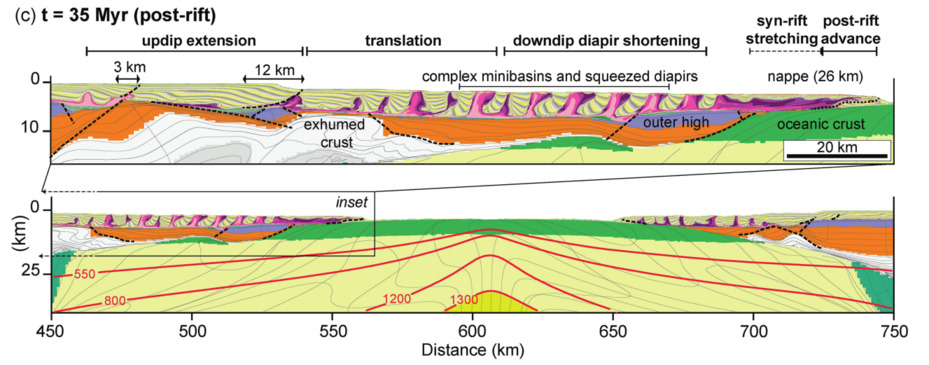
\includegraphics[height=5cm]{images/mycodes/pihg22a_img}
\end{center}

%--------------------------------------------------------------------------------------------------
\item {\it Coupling Crustal-Scale Rift Architecture With Passive Margin
Salt Tectonics: A Geodynamic Modeling Approach}, 
L.M. Pichel, R.S. Huismans, R. Gawthorpe, J.I. Faleide and Th. Theunissen, JGR, 127, 2022. \cite{pihg22b}
\begin{center}
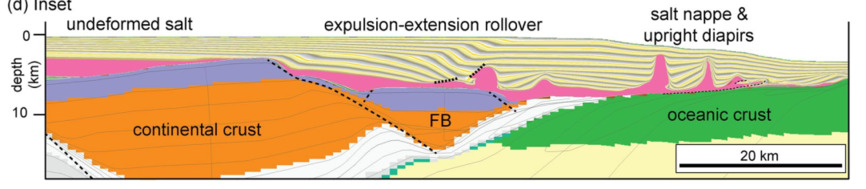
\includegraphics[height=3cm]{images/mycodes/pihg22b_img}
\end{center}

%--------------------------------------------------------------------------------------------------
\item {\it How post-­salt sediment flux and progradation rate
influence salt tectonics on rifted margins: Insights from
geodynamic modelling},
L.M. Pichel, R.S. Huismans, R. Gawthorpe and  J.I. Faleide, Basin Research, 2023. \cite{pihg23}
\begin{center}
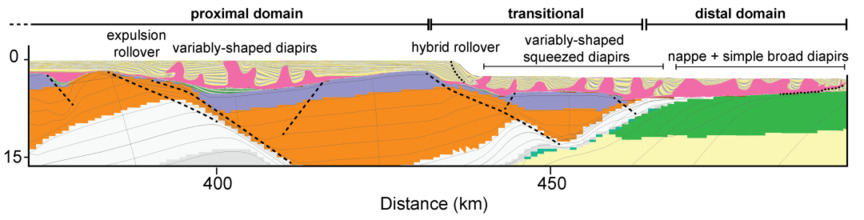
\includegraphics[height=3cm]{images/mycodes/pihg23_img}
\end{center}

\item {\it A Three-Field Formulation for Two-Phase Flow in
Geodynamic Modeling: Toward the Zero-Porosity Limit},
Gang Lu, Dave A. May and Ritske S. Huismans, 
Journal of Geophysical Research: Solid Earth, 2024. \cite{lumh24}


\end{itemize}


%--------------------------------------------------------------------------------------------------
%--------------------------------------------------------------------------------------------------
%--------------------------------------------------------------------------------------------------
%--------------------------------------------------------------------------------------------------

Upon my arrival at Utrecht University in 2012 I started working an a more flexible code, called \elefant, 
which has since very much diverged from \fantom.

\begin{itemize}
\item {\it The effect of obliquity on temperature in subduction zones: insights from 3-D numerical modeling}, 
A. Plunder, C. Thieulot and D.J.J. van Hinsbergen, Solid Earth 9, 759-776, 2018. \url{https://doi.org/10.5194/se-9-759-2018}

\begin{center}
\includegraphics[height=3.5cm]{images/mycodes/pltv18_img}
\end{center}


\item {\it Analytical solution for viscous incompressible Stokes flow in a spherical shell}, 
C. Thieulot, Solid Earth 8, 1181-1191, 2017. \url{https://doi.org/10.5194/se-8-1181-2017}

\begin{center}
\includegraphics[height=3cm]{images/mycodes/thie17_img}
\end{center}



\item  {\it Lithosphere erosion and continental breakup: interaction of extension, plume upwelling and melting}, 
A. Lavecchia, C. Thieulot, F. Beekman, S. Cloetingh and S. Clark, E.P.S.L. 467, p89-98, 2017.

\begin{center}
\includegraphics[height=3cm]{images/mycodes/latv17_img}
\end{center}


\item {\it Benchmarking numerical models of brittle thrust wedges}, 
Susanne J.H. Buiter, Guido Schreurs, Markus Albertz, Taras V. Gerya, Boris Kaus,
Walter Landry, Laetitia le Pourhiet, Yury Mishin, David L. Egholm, Michele Cooke,
Bertrand Maillot, Cedric Thieulot, Tony Crook, Dave May, Pauline Souloumiac, Christopher Beaumont
Journal of Structural Geology 92, p140-177, 2016. \url{https://doi:10.1016/j.jsg.2016.03.003}

\begin{center}
\includegraphics[height=1.8cm]{images/mycodes/busa16_img}
\end{center}


\item {\it A community benchmark for viscoplastic thermal convection in a 2-D square box}, 
N. Tosi, C. Stein, L. Noack, C. Huettig, P. Maierova, H. Samuel, D.R. Davies, C.R. Wilson, S.C. Kramer, C. Thieulot, A. Glerum, M. Fraters, W. Spakman, A. Rozel, P.J. Tackley, Geochem. Geophys. Geosyst. 16, doi:10.1002/2015GC005807, 2015.

\begin{center}
\includegraphics[height=3cm]{images/mycodes/tosn15_img}
\end{center}


\item {\it Dynamics of intraoceanic subduction initiation: 1. Oceanic detachment fault inversion and the formation of supra-subduction zone ophiolites}, M. Maffione, C. Thieulot, D.J.J. van Hinsbergen, A. Morris, O. Pluemper and W. Spakman, Geochem. Geophys. Geosyst. 16, p1753-1770, 2015.

\begin{center}
\includegraphics[height=1.8cm]{images/mycodes/matv15_img}
\end{center}

\item {\it The Geodynamic World Builder: a solution for complex initial conditions in numerical modelling},
M. Fraters, C. Thieulot, A. van den Berg and W. Spakman,
Solid Earth, \url{https://doi.org/10.5194/se-2019-24}, 2019.

\begin{center}
\includegraphics[height=2.8cm]{images/mycodes/frtv19_img}
\end{center}


\end{itemize}


\begin{itemize}
\item {\it GHOST: Geoscientific Hollow Sphere Tessellation}, 
C. Thieulot, Solid Earth, 9, 1169-1177, 2018. \url{https://doi.org/10.5194/se-9-1169-2018}

\begin{center}
\includegraphics[height=3cm]{images/mycodes/shell_HS06}
\includegraphics[height=3cm]{images/mycodes/shell_HS12}
\includegraphics[height=3cm]{images/mycodes/shell_HS20}
\end{center}


title={Long-term coupling and feedback between tectonics and surface processes 
during non-volcanic rifted margin formation},
author={Theunissen, Thomas and Huismans, Ritske S},
journal={Journal of Geophysical Research: Solid Earth},

\end{itemize}



\printbibliography
\end{document}
%%%%%%%%%%%%%%%%%%%%%%%%%%%%%%%%%%%%%%%%%%%%%%%%%%%%%%%%%%%
